\documentclass[twoside]{book}

% Packages required by doxygen
\usepackage{fixltx2e}
\usepackage{calc}
\usepackage{doxygen}
\usepackage[export]{adjustbox} % also loads graphicx
\usepackage{graphicx}
\usepackage[utf8]{inputenc}
\usepackage{makeidx}
\usepackage{multicol}
\usepackage{multirow}
\PassOptionsToPackage{warn}{textcomp}
\usepackage{textcomp}
\usepackage[nointegrals]{wasysym}
\usepackage[table]{xcolor}

% Font selection
\usepackage[T1]{fontenc}
\usepackage[scaled=.90]{helvet}
\usepackage{courier}
\usepackage{amssymb}
\usepackage{sectsty}
\renewcommand{\familydefault}{\sfdefault}
\allsectionsfont{%
  \fontseries{bc}\selectfont%
  \color{darkgray}%
}
\renewcommand{\DoxyLabelFont}{%
  \fontseries{bc}\selectfont%
  \color{darkgray}%
}
\newcommand{\+}{\discretionary{\mbox{\scriptsize$\hookleftarrow$}}{}{}}

% Page & text layout
\usepackage{geometry}
\geometry{%
  a4paper,%
  top=2.5cm,%
  bottom=2.5cm,%
  left=2.5cm,%
  right=2.5cm%
}
\tolerance=750
\hfuzz=15pt
\hbadness=750
\setlength{\emergencystretch}{15pt}
\setlength{\parindent}{0cm}
\setlength{\parskip}{3ex plus 2ex minus 2ex}
\makeatletter
\renewcommand{\paragraph}{%
  \@startsection{paragraph}{4}{0ex}{-1.0ex}{1.0ex}{%
    \normalfont\normalsize\bfseries\SS@parafont%
  }%
}
\renewcommand{\subparagraph}{%
  \@startsection{subparagraph}{5}{0ex}{-1.0ex}{1.0ex}{%
    \normalfont\normalsize\bfseries\SS@subparafont%
  }%
}
\makeatother

% Headers & footers
\usepackage{fancyhdr}
\pagestyle{fancyplain}
\fancyhead[LE]{\fancyplain{}{\bfseries\thepage}}
\fancyhead[CE]{\fancyplain{}{}}
\fancyhead[RE]{\fancyplain{}{\bfseries\leftmark}}
\fancyhead[LO]{\fancyplain{}{\bfseries\rightmark}}
\fancyhead[CO]{\fancyplain{}{}}
\fancyhead[RO]{\fancyplain{}{\bfseries\thepage}}
\fancyfoot[LE]{\fancyplain{}{}}
\fancyfoot[CE]{\fancyplain{}{}}
\fancyfoot[RE]{\fancyplain{}{\bfseries\scriptsize Generated by Doxygen }}
\fancyfoot[LO]{\fancyplain{}{\bfseries\scriptsize Generated by Doxygen }}
\fancyfoot[CO]{\fancyplain{}{}}
\fancyfoot[RO]{\fancyplain{}{}}
\renewcommand{\footrulewidth}{0.4pt}
\renewcommand{\chaptermark}[1]{%
  \markboth{#1}{}%
}
\renewcommand{\sectionmark}[1]{%
  \markright{\thesection\ #1}%
}

% Indices & bibliography
\usepackage{natbib}
\usepackage[titles]{tocloft}
\setcounter{tocdepth}{3}
\setcounter{secnumdepth}{5}
\makeindex

% Hyperlinks (required, but should be loaded last)
\usepackage{ifpdf}
\ifpdf
  \usepackage[pdftex,pagebackref=true]{hyperref}
\else
  \usepackage[ps2pdf,pagebackref=true]{hyperref}
\fi
\hypersetup{%
  colorlinks=true,%
  linkcolor=blue,%
  citecolor=blue,%
  unicode%
}

% Custom commands
\newcommand{\clearemptydoublepage}{%
  \newpage{\pagestyle{empty}\cleardoublepage}%
}

\usepackage{caption}
\captionsetup{labelsep=space,justification=centering,font={bf},singlelinecheck=off,skip=4pt,position=top}

%===== C O N T E N T S =====

\begin{document}

% Titlepage & ToC
\hypersetup{pageanchor=false,
             bookmarksnumbered=true,
             pdfencoding=unicode
            }
\pagenumbering{alph}
\begin{titlepage}
\vspace*{7cm}
\begin{center}%
{\Large real\+\_\+time\+\_\+tools }\\
\vspace*{1cm}
{\large Generated by Doxygen 1.8.13}\\
\end{center}
\end{titlepage}
\clearemptydoublepage
\pagenumbering{roman}
\tableofcontents
\clearemptydoublepage
\pagenumbering{arabic}
\hypersetup{pageanchor=true}

%--- Begin generated contents ---
\chapter{real\+\_\+time\+\_\+tools}
\label{index}\hypertarget{index}{}\subsection*{What is it}

This package contains a set of examples of demos and unit tests in c++ supported by the continuous integration. It also contains the coding guidelines setup in the \href{https://wp.nyu.edu/machinesinmotion/}{\tt machines-\/in-\/motion} group.

\subsection*{Authors}


\begin{DoxyItemize}
\item Vincent Berenz
\item Maximilien Naveau
\end{DoxyItemize}

\subsection*{Copyrights}

Copyright (c) 2019, New York University and Max Planck Gesellschaft.

\subsection*{License}

License B\+S\+D-\/3-\/\+Clause 
\chapter{Todo List}
\label{todo}
\Hypertarget{todo}

\begin{DoxyRefList}
\item[\label{todo__todo000001}%
\Hypertarget{todo__todo000001}%
Member \hyperlink{classreal__time__tools_1_1RealTimeThreadParameters_a50e8eae41f8284867f073aa802d9afa2}{real\+\_\+time\+\_\+tools\+:\+:Real\+Time\+Thread\+Parameters\+:\+:delay\+\_\+ns\+\_\+} ]Unknow Xenomai parameter  
\item[\label{todo__todo000003}%
\Hypertarget{todo__todo000003}%
Member \hyperlink{classreal__time__tools_1_1SingletypeThreadsafeObject_a1f852a4b68d3a0ff112cb9c5d7c6b33e}{real\+\_\+time\+\_\+tools\+:\+:Singletype\+Threadsafe\+Object$<$ Type, S\+I\+ZE $>$\+:\+:set} (Type datum)]\char`\"{}\+This is used for backward comaptibility.\char`\"{}, Manuel Which bakward? 
\item[\label{todo__todo000002}%
\Hypertarget{todo__todo000002}%
Member \hyperlink{classreal__time__tools_1_1ThreadsafeHistoryInterface_a3304dfddbf562b835745be3ff363ab17}{real\+\_\+time\+\_\+tools\+:\+:Threadsafe\+History\+Interface$<$ Type $>$\+:\+:add} ()=0]Manuel, could you delete this class or provide an implementation? 
\end{DoxyRefList}
\chapter{License}
\label{license}
\Hypertarget{license}

\begin{DoxyRefList}
\item[\label{license__license000001}%
\Hypertarget{license__license000001}%
File \hyperlink{yaml__cpp__fwd_8hpp}{yaml\+\_\+cpp\+\_\+fwd.hpp} ]License B\+S\+D-\/3-\/\+Clause  
\item[\label{license__license000002}%
\Hypertarget{license__license000002}%
File \hyperlink{yaml__eigen_8h}{yaml\+\_\+eigen.h} ]License B\+S\+D-\/3-\/\+Clause  
\item[\label{license__license000003}%
\Hypertarget{license__license000003}%
File \hyperlink{yaml__tools_8hpp}{yaml\+\_\+tools.hpp} ]License B\+S\+D-\/3-\/\+Clause 
\end{DoxyRefList}
\chapter{Hierarchical Index}
\section{Class Hierarchy}
This inheritance list is sorted roughly, but not completely, alphabetically\+:\begin{DoxyCompactList}
\item array\+\_\+members\begin{DoxyCompactList}
\item \contentsline{section}{shared\+\_\+memory\+:\+:array$<$ T, S\+I\+ZE $>$}{\pageref{classshared__memory_1_1array}}{}
\end{DoxyCompactList}
\item \contentsline{section}{shared\+\_\+memory\+:\+:Condition\+Variable}{\pageref{classshared__memory_1_1ConditionVariable}}{}
\item \contentsline{section}{Config}{\pageref{classConfig}}{}
\item exception\begin{DoxyCompactList}
\item \contentsline{section}{shared\+\_\+memory\+:\+:Allocation\+\_\+exception}{\pageref{classshared__memory_1_1Allocation__exception}}{}
\item \contentsline{section}{shared\+\_\+memory\+:\+:Memory\+\_\+overflow\+\_\+exception}{\pageref{classshared__memory_1_1Memory__overflow__exception}}{}
\item \contentsline{section}{shared\+\_\+memory\+:\+:Not\+\_\+consumed\+\_\+exception}{\pageref{classshared__memory_1_1Not__consumed__exception}}{}
\item \contentsline{section}{shared\+\_\+memory\+:\+:Unexpected\+\_\+map\+\_\+key$<$ Key $>$}{\pageref{classshared__memory_1_1Unexpected__map__key}}{}
\item \contentsline{section}{shared\+\_\+memory\+:\+:Unexpected\+\_\+size\+\_\+exception}{\pageref{classshared__memory_1_1Unexpected__size__exception}}{}
\end{DoxyCompactList}
\item \contentsline{section}{shared\+\_\+memory\+:\+:Exchange\+\_\+manager\+\_\+consumer$<$ Serializable, Q\+U\+E\+U\+E\+\_\+\+S\+I\+ZE $>$}{\pageref{classshared__memory_1_1Exchange__manager__consumer}}{}
\item \contentsline{section}{shared\+\_\+memory\+:\+:Exchange\+\_\+manager\+\_\+producer$<$ Serializable, Q\+U\+E\+U\+E\+\_\+\+S\+I\+ZE $>$}{\pageref{classshared__memory_1_1Exchange__manager__producer}}{}
\item \contentsline{section}{shared\+\_\+memory\+:\+:Four\+\_\+int\+\_\+values}{\pageref{classshared__memory_1_1Four__int__values}}{}
\item \contentsline{section}{shared\+\_\+memory\+:\+:Item$<$ S\+I\+ZE $>$}{\pageref{classshared__memory_1_1Item}}{}
\item \contentsline{section}{shared\+\_\+memory\+:\+:Lock}{\pageref{classshared__memory_1_1Lock}}{}
\item \contentsline{section}{shared\+\_\+memory\+:\+:Locked\+Condition\+Variable}{\pageref{classshared__memory_1_1LockedConditionVariable}}{}
\item \contentsline{section}{Measure\+Time}{\pageref{structMeasureTime}}{}
\item \contentsline{section}{shared\+\_\+memory\+:\+:Mutex}{\pageref{classshared__memory_1_1Mutex}}{}
\item \contentsline{section}{shared\+\_\+memory\+:\+:Segment\+Info}{\pageref{classshared__memory_1_1SegmentInfo}}{}
\item \contentsline{section}{Serializable$<$ S\+I\+ZE $>$}{\pageref{classSerializable}}{}
\item \contentsline{section}{shared\+\_\+memory\+:\+:Serializable\+\_\+exchange$<$ Serializable $>$}{\pageref{classshared__memory_1_1Serializable__exchange}}{}
\item \contentsline{section}{Serializable\+Example}{\pageref{classSerializableExample}}{}
\item \contentsline{section}{shared\+\_\+memory\+:\+:Serializer$<$ Serializable $>$}{\pageref{classshared__memory_1_1Serializer}}{}
\item \contentsline{section}{shared\+\_\+memory\+:\+:Shared\+Memory\+Segment}{\pageref{classshared__memory_1_1SharedMemorySegment}}{}
\item \contentsline{section}{shared\+\_\+memory\+:\+:Shm\+Type\+Helper$<$ Elem\+Type $>$}{\pageref{structshared__memory_1_1ShmTypeHelper}}{}
\end{DoxyCompactList}

\chapter{Class Index}
\section{Class List}
Here are the classes, structs, unions and interfaces with brief descriptions\+:\begin{DoxyCompactList}
\item\contentsline{section}{\hyperlink{classshared__memory_1_1Allocation__exception}{shared\+\_\+memory\+::\+Allocation\+\_\+exception} }{\pageref{classshared__memory_1_1Allocation__exception}}{}
\item\contentsline{section}{\hyperlink{classshared__memory_1_1array}{shared\+\_\+memory\+::array$<$ T, S\+I\+Z\+E $>$} \\*Implement a shared array stored on a shared memory segment }{\pageref{classshared__memory_1_1array}}{}
\item\contentsline{section}{\hyperlink{classshared__memory_1_1internal_1_1array__members}{shared\+\_\+memory\+::internal\+::array\+\_\+members$<$ T, S\+I\+Z\+E, Enable $>$} }{\pageref{classshared__memory_1_1internal_1_1array__members}}{}
\item\contentsline{section}{\hyperlink{classshared__memory_1_1internal_1_1array__members_3_01T_00_010_00_01typename_01std_1_1enable__ifb2fde5f96702510d664610c5e9570772}{shared\+\_\+memory\+::internal\+::array\+\_\+members$<$ T, 0, typename std\+::enable\+\_\+if$<$ std\+::is\+\_\+fundamental$<$ T $>$\+::value $>$\+::type $>$} }{\pageref{classshared__memory_1_1internal_1_1array__members_3_01T_00_010_00_01typename_01std_1_1enable__ifb2fde5f96702510d664610c5e9570772}}{}
\item\contentsline{section}{\hyperlink{classshared__memory_1_1internal_1_1array__members_3_01T_00_01SIZE_00_01typename_01std_1_1enable_de9984c52d14535c26d7a424fbd87fe2}{shared\+\_\+memory\+::internal\+::array\+\_\+members$<$ T, S\+I\+Z\+E, typename std\+::enable\+\_\+if$<$ std\+::is\+\_\+fundamental$<$ T $>$\+::value \&\&\+S\+I\+Z\+E!=0 $>$\+::type $>$} }{\pageref{classshared__memory_1_1internal_1_1array__members_3_01T_00_01SIZE_00_01typename_01std_1_1enable_de9984c52d14535c26d7a424fbd87fe2}}{}
\item\contentsline{section}{\hyperlink{classshared__memory_1_1ConditionVariable}{shared\+\_\+memory\+::\+Condition\+Variable} }{\pageref{classshared__memory_1_1ConditionVariable}}{}
\item\contentsline{section}{\hyperlink{classConfig}{Config} }{\pageref{classConfig}}{}
\item\contentsline{section}{\hyperlink{classshared__memory_1_1Exchange__manager__consumer}{shared\+\_\+memory\+::\+Exchange\+\_\+manager\+\_\+consumer$<$ Serializable, Q\+U\+E\+U\+E\+\_\+\+S\+I\+Z\+E $>$} }{\pageref{classshared__memory_1_1Exchange__manager__consumer}}{}
\item\contentsline{section}{\hyperlink{classshared__memory_1_1internal_1_1Exchange__manager__memory}{shared\+\_\+memory\+::internal\+::\+Exchange\+\_\+manager\+\_\+memory$<$ Serializable, Q\+U\+E\+U\+E\+\_\+\+S\+I\+Z\+E $>$} }{\pageref{classshared__memory_1_1internal_1_1Exchange__manager__memory}}{}
\item\contentsline{section}{\hyperlink{classshared__memory_1_1Exchange__manager__producer}{shared\+\_\+memory\+::\+Exchange\+\_\+manager\+\_\+producer$<$ Serializable, Q\+U\+E\+U\+E\+\_\+\+S\+I\+Z\+E $>$} }{\pageref{classshared__memory_1_1Exchange__manager__producer}}{}
\item\contentsline{section}{\hyperlink{classshared__memory_1_1Four__int__values}{shared\+\_\+memory\+::\+Four\+\_\+int\+\_\+values} \\*Example of an instance that can be serialized }{\pageref{classshared__memory_1_1Four__int__values}}{}
\item\contentsline{section}{\hyperlink{classshared__memory_1_1Item}{shared\+\_\+memory\+::\+Item$<$ S\+I\+Z\+E $>$} }{\pageref{classshared__memory_1_1Item}}{}
\item\contentsline{section}{\hyperlink{classshared__memory_1_1Lock}{shared\+\_\+memory\+::\+Lock} \\*A scope lock object for locking a shared memory mutex, to use for example with a shared memory condition variable }{\pageref{classshared__memory_1_1Lock}}{}
\item\contentsline{section}{\hyperlink{classshared__memory_1_1LockedConditionVariable}{shared\+\_\+memory\+::\+Locked\+Condition\+Variable} \\*Here as a anonymous layer on top of the boost intersprocess condition variable labrary }{\pageref{classshared__memory_1_1LockedConditionVariable}}{}
\item\contentsline{section}{\hyperlink{structMeasureTime}{Measure\+Time} }{\pageref{structMeasureTime}}{}
\item\contentsline{section}{\hyperlink{classshared__memory_1_1Memory__overflow__exception}{shared\+\_\+memory\+::\+Memory\+\_\+overflow\+\_\+exception} }{\pageref{classshared__memory_1_1Memory__overflow__exception}}{}
\item\contentsline{section}{\hyperlink{classshared__memory_1_1Mutex}{shared\+\_\+memory\+::\+Mutex} }{\pageref{classshared__memory_1_1Mutex}}{}
\item\contentsline{section}{\hyperlink{classshared__memory_1_1Not__consumed__exception}{shared\+\_\+memory\+::\+Not\+\_\+consumed\+\_\+exception} }{\pageref{classshared__memory_1_1Not__consumed__exception}}{}
\item\contentsline{section}{\hyperlink{classshared__memory_1_1SegmentInfo}{shared\+\_\+memory\+::\+Segment\+Info} \\*Encapsulate information related to a shared memory segment }{\pageref{classshared__memory_1_1SegmentInfo}}{}
\item\contentsline{section}{\hyperlink{classSerializable}{Serializable$<$ S\+I\+Z\+E $>$} }{\pageref{classSerializable}}{}
\item\contentsline{section}{\hyperlink{classshared__memory_1_1Serializable__exchange}{shared\+\_\+memory\+::\+Serializable\+\_\+exchange$<$ Serializable $>$} }{\pageref{classshared__memory_1_1Serializable__exchange}}{}
\item\contentsline{section}{\hyperlink{classSerializableExample}{Serializable\+Example} }{\pageref{classSerializableExample}}{}
\item\contentsline{section}{\hyperlink{classshared__memory_1_1internal_1_1Serialized__read}{shared\+\_\+memory\+::internal\+::\+Serialized\+\_\+read$<$ Serializable $>$} }{\pageref{classshared__memory_1_1internal_1_1Serialized__read}}{}
\item\contentsline{section}{\hyperlink{classshared__memory_1_1internal_1_1Serialized__write}{shared\+\_\+memory\+::internal\+::\+Serialized\+\_\+write$<$ Serializable $>$} }{\pageref{classshared__memory_1_1internal_1_1Serialized__write}}{}
\item\contentsline{section}{\hyperlink{classshared__memory_1_1Serializer}{shared\+\_\+memory\+::\+Serializer$<$ Serializable $>$} }{\pageref{classshared__memory_1_1Serializer}}{}
\item\contentsline{section}{\hyperlink{classshared__memory_1_1SharedMemorySegment}{shared\+\_\+memory\+::\+Shared\+Memory\+Segment} \\*The \hyperlink{classshared__memory_1_1SharedMemorySegment}{Shared\+Memory\+Segment} contains the pointers of the shared objects in on shared memrory segment }{\pageref{classshared__memory_1_1SharedMemorySegment}}{}
\item\contentsline{section}{\hyperlink{structshared__memory_1_1ShmTypeHelper}{shared\+\_\+memory\+::\+Shm\+Type\+Helper$<$ Elem\+Type $>$} \\*\hyperlink{structshared__memory_1_1ShmTypeHelper}{Shm\+Type\+Helper} is a small struct that allow the definition of templated typedef }{\pageref{structshared__memory_1_1ShmTypeHelper}}{}
\item\contentsline{section}{\hyperlink{classshared__memory_1_1Unexpected__map__key}{shared\+\_\+memory\+::\+Unexpected\+\_\+map\+\_\+key$<$ Key $>$} }{\pageref{classshared__memory_1_1Unexpected__map__key}}{}
\item\contentsline{section}{\hyperlink{classshared__memory_1_1Unexpected__size__exception}{shared\+\_\+memory\+::\+Unexpected\+\_\+size\+\_\+exception} }{\pageref{classshared__memory_1_1Unexpected__size__exception}}{}
\end{DoxyCompactList}

\chapter{File Index}
\section{File List}
Here is a list of all documented files with brief descriptions\+:\begin{DoxyCompactList}
\item\contentsline{section}{include/dg\+\_\+blmc\+\_\+robots/\hyperlink{common__header_8hpp}{common\+\_\+header.\+hpp} }{\pageref{common__header_8hpp}}{}
\item\contentsline{section}{include/dg\+\_\+blmc\+\_\+robots/\hyperlink{dgm__single__motor_8hpp}{dgm\+\_\+single\+\_\+motor.\+hpp} }{\pageref{dgm__single__motor_8hpp}}{}
\item\contentsline{section}{include/dg\+\_\+blmc\+\_\+robots/{\bfseries dgm\+\_\+solo12.\+hpp} }{\pageref{dgm__solo12_8hpp}}{}
\item\contentsline{section}{include/dg\+\_\+blmc\+\_\+robots/{\bfseries dgm\+\_\+solo8.\+hpp} }{\pageref{dgm__solo8_8hpp}}{}
\item\contentsline{section}{include/dg\+\_\+blmc\+\_\+robots/{\bfseries dgm\+\_\+solo8ti.\+hpp} }{\pageref{dgm__solo8ti_8hpp}}{}
\item\contentsline{section}{include/dg\+\_\+blmc\+\_\+robots/{\bfseries dgm\+\_\+solo\+\_\+simple\+\_\+simu.\+hpp} }{\pageref{dgm__solo__simple__simu_8hpp}}{}
\item\contentsline{section}{include/dg\+\_\+blmc\+\_\+robots/\hyperlink{dgm__stuggihop_8hpp}{dgm\+\_\+stuggihop.\+hpp} }{\pageref{dgm__stuggihop_8hpp}}{}
\item\contentsline{section}{include/dg\+\_\+blmc\+\_\+robots/{\bfseries dgm\+\_\+teststand.\+hpp} }{\pageref{dgm__teststand_8hpp}}{}
\item\contentsline{section}{src/\hyperlink{dgm__solo__simple__simu_8cpp}{dgm\+\_\+solo\+\_\+simple\+\_\+simu.\+cpp} \\*The hardware wrapper of the solo naive simulation }{\pageref{dgm__solo__simple__simu_8cpp}}{}
\item\contentsline{section}{src/\hyperlink{dgm__stuggihop_8cpp}{dgm\+\_\+stuggihop.\+cpp} \\*D\+GM wrapper around the stuggihop robot }{\pageref{dgm__stuggihop_8cpp}}{}
\end{DoxyCompactList}

\chapter{Class Documentation}
\hypertarget{classreal__time__tools_1_1CheckpointTimer}{}\section{real\+\_\+time\+\_\+tools\+:\+:Checkpoint\+Timer$<$ N\+U\+M\+\_\+\+C\+H\+E\+C\+K\+P\+O\+I\+N\+TS, E\+N\+A\+B\+L\+ED $>$ Class Template Reference}
\label{classreal__time__tools_1_1CheckpointTimer}\index{real\+\_\+time\+\_\+tools\+::\+Checkpoint\+Timer$<$ N\+U\+M\+\_\+\+C\+H\+E\+C\+K\+P\+O\+I\+N\+T\+S, E\+N\+A\+B\+L\+E\+D $>$@{real\+\_\+time\+\_\+tools\+::\+Checkpoint\+Timer$<$ N\+U\+M\+\_\+\+C\+H\+E\+C\+K\+P\+O\+I\+N\+T\+S, E\+N\+A\+B\+L\+E\+D $>$}}


\hyperlink{classreal__time__tools_1_1Timer}{Timer} to measure code execution time with \char`\"{}checkpoints\char`\"{}.  




{\ttfamily \#include $<$checkpoint\+\_\+timer.\+hpp$>$}

\subsection*{Public Member Functions}
\begin{DoxyCompactItemize}
\item 
\mbox{\Hypertarget{classreal__time__tools_1_1CheckpointTimer_ad93a12cb74103528c8db4e7b1745eae6}\label{classreal__time__tools_1_1CheckpointTimer_ad93a12cb74103528c8db4e7b1745eae6}} 
void \hyperlink{classreal__time__tools_1_1CheckpointTimer_ad93a12cb74103528c8db4e7b1745eae6}{start} ()
\begin{DoxyCompactList}\small\item\em Start timer iteration. \end{DoxyCompactList}\item 
void \hyperlink{classreal__time__tools_1_1CheckpointTimer_a6e91b61b72c433a220b1bddb7a634bf5}{checkpoint} (const std\+::string \&checkpoint\+\_\+name)
\begin{DoxyCompactList}\small\item\em Set checkpoint for time measurement. \end{DoxyCompactList}\item 
\mbox{\Hypertarget{classreal__time__tools_1_1CheckpointTimer_a73e001fa40a76ce5fd917a2dfcd09555}\label{classreal__time__tools_1_1CheckpointTimer_a73e001fa40a76ce5fd917a2dfcd09555}} 
void \hyperlink{classreal__time__tools_1_1CheckpointTimer_a73e001fa40a76ce5fd917a2dfcd09555}{print\+\_\+statistics} () const
\begin{DoxyCompactList}\small\item\em Print results of time measurements. \end{DoxyCompactList}\end{DoxyCompactItemize}
\subsection*{Private Attributes}
\begin{DoxyCompactItemize}
\item 
std\+::array$<$ \hyperlink{classreal__time__tools_1_1Timer}{real\+\_\+time\+\_\+tools\+::\+Timer}, N\+U\+M\+\_\+\+C\+H\+E\+C\+K\+P\+O\+I\+N\+TS+1 $>$ \hyperlink{classreal__time__tools_1_1CheckpointTimer_a0abbead69aaf780b649f6af01f50cc62}{timers\+\_\+}
\begin{DoxyCompactList}\small\item\em Timers used for the different checkpoints. \end{DoxyCompactList}\item 
\mbox{\Hypertarget{classreal__time__tools_1_1CheckpointTimer_afbb3abc9e62174d6046f6abb294a120f}\label{classreal__time__tools_1_1CheckpointTimer_afbb3abc9e62174d6046f6abb294a120f}} 
std\+::array$<$ std\+::string, N\+U\+M\+\_\+\+C\+H\+E\+C\+K\+P\+O\+I\+N\+TS+1 $>$ \hyperlink{classreal__time__tools_1_1CheckpointTimer_afbb3abc9e62174d6046f6abb294a120f}{checkpoint\+\_\+names\+\_\+}
\begin{DoxyCompactList}\small\item\em Names of the checkpoints. \end{DoxyCompactList}\item 
\mbox{\Hypertarget{classreal__time__tools_1_1CheckpointTimer_a07ae61ac85e755629625cc32416f2631}\label{classreal__time__tools_1_1CheckpointTimer_a07ae61ac85e755629625cc32416f2631}} 
size\+\_\+t \hyperlink{classreal__time__tools_1_1CheckpointTimer_a07ae61ac85e755629625cc32416f2631}{current\+\_\+checkpoint\+\_\+} = 1
\begin{DoxyCompactList}\small\item\em Index of the current checkpoint. \end{DoxyCompactList}\end{DoxyCompactItemize}


\subsection{Detailed Description}
\subsubsection*{template$<$size\+\_\+t N\+U\+M\+\_\+\+C\+H\+E\+C\+K\+P\+O\+I\+N\+TS, bool E\+N\+A\+B\+L\+ED = true$>$\newline
class real\+\_\+time\+\_\+tools\+::\+Checkpoint\+Timer$<$ N\+U\+M\+\_\+\+C\+H\+E\+C\+K\+P\+O\+I\+N\+T\+S, E\+N\+A\+B\+L\+E\+D $>$}

\hyperlink{classreal__time__tools_1_1Timer}{Timer} to measure code execution time with \char`\"{}checkpoints\char`\"{}. 

This timer is meant to be used for measuring execution time of a loop. It measures time between calls of the {\ttfamily start} method, so by calling this at the beginning of the loop, you get the execution time of the full iteration. Further, you can define \char`\"{}checkpoints\char`\"{} within the loop to measure time of separate steps in the loop. Call the {\ttfamily checkpoint} method after the code that is associated with it. For each checkpoint, the time elapsed since the last checkpoint is measured ({\ttfamily start} counts as a checkpoint in this regard).

Example\+: 
\begin{DoxyCodeInclude}

    \textcolor{comment}{// set second template argument to false to disable timer}
    \hyperlink{classreal__time__tools_1_1CheckpointTimer}{real\_time\_tools::CheckpointTimer<3, true>} timer;

    \textcolor{keywordflow}{for} (\textcolor{keywordtype}{int} i = 0; i < 1000; i++)
    \{
        timer.\hyperlink{classreal__time__tools_1_1CheckpointTimer_ad93a12cb74103528c8db4e7b1745eae6}{start}();

        \hyperlink{demo__checkpoint__timer_8cpp_a02fd73d861ef2e4aabb38c0c9ff82947}{init}();
        timer.\hyperlink{classreal__time__tools_1_1CheckpointTimer_a6e91b61b72c433a220b1bddb7a634bf5}{checkpoint}(\textcolor{stringliteral}{"initialize"});

        \hyperlink{demo__checkpoint__timer_8cpp_acb546a895e868f1a8fb9cb4b5a210f42}{do\_some\_stuff}();
        timer.\hyperlink{classreal__time__tools_1_1CheckpointTimer_a6e91b61b72c433a220b1bddb7a634bf5}{checkpoint}(\textcolor{stringliteral}{"do some stuff"});

        \hyperlink{demo__checkpoint__timer_8cpp_a609e6537df0c7eb15c1f5b4e02fbe0ed}{write\_log}();
        timer.\hyperlink{classreal__time__tools_1_1CheckpointTimer_a6e91b61b72c433a220b1bddb7a634bf5}{checkpoint}(\textcolor{stringliteral}{"logging"});

        \textcolor{comment}{// print the timing results every 100 iterations}
        \textcolor{keywordflow}{if} (i % 100 == 0 && i > 0)
        \{
            timer.\hyperlink{classreal__time__tools_1_1CheckpointTimer_a73e001fa40a76ce5fd917a2dfcd09555}{print\_statistics}();
        \}
    \}

\end{DoxyCodeInclude}
 
\begin{DoxyTemplParams}{Template Parameters}
{\em N\+U\+M\+\_\+\+C\+H\+E\+C\+K\+P\+O\+I\+N\+TS} & Number of checkpoints. \\
\hline
{\em E\+N\+A\+B\+L\+ED} & Set to false, to disable timer. Method calls will have no effect (and should hopefully be optimized away by the compiler). \\
\hline
\end{DoxyTemplParams}
\begin{Desc}
\item[Examples\+: ]\par
\hyperlink{demo_checkpoint_timer_8cpp-example}{demo\+\_\+checkpoint\+\_\+timer.\+cpp}.\end{Desc}


\subsection{Member Function Documentation}
\mbox{\Hypertarget{classreal__time__tools_1_1CheckpointTimer_a6e91b61b72c433a220b1bddb7a634bf5}\label{classreal__time__tools_1_1CheckpointTimer_a6e91b61b72c433a220b1bddb7a634bf5}} 
\index{real\+\_\+time\+\_\+tools\+::\+Checkpoint\+Timer@{real\+\_\+time\+\_\+tools\+::\+Checkpoint\+Timer}!checkpoint@{checkpoint}}
\index{checkpoint@{checkpoint}!real\+\_\+time\+\_\+tools\+::\+Checkpoint\+Timer@{real\+\_\+time\+\_\+tools\+::\+Checkpoint\+Timer}}
\subsubsection{\texorpdfstring{checkpoint()}{checkpoint()}}
{\footnotesize\ttfamily template$<$size\+\_\+t N\+U\+M\+\_\+\+C\+H\+E\+C\+K\+P\+O\+I\+N\+TS, bool E\+N\+A\+B\+L\+ED$>$ \\
void Checkpoint\+Timer\+::checkpoint (\begin{DoxyParamCaption}\item[{const std\+::string \&}]{checkpoint\+\_\+name }\end{DoxyParamCaption})}



Set checkpoint for time measurement. 

Measures time from the last call of \hyperlink{classreal__time__tools_1_1CheckpointTimer_ad93a12cb74103528c8db4e7b1745eae6}{start()} or \hyperlink{classreal__time__tools_1_1CheckpointTimer_a6e91b61b72c433a220b1bddb7a634bf5}{checkpoint()} until this call. The given name is used when printing the results.


\begin{DoxyParams}{Parameters}
{\em checkpoint\+\_\+name} & Name of the checkpoint (used for printing results) \\
\hline
\end{DoxyParams}


\subsection{Member Data Documentation}
\mbox{\Hypertarget{classreal__time__tools_1_1CheckpointTimer_a0abbead69aaf780b649f6af01f50cc62}\label{classreal__time__tools_1_1CheckpointTimer_a0abbead69aaf780b649f6af01f50cc62}} 
\index{real\+\_\+time\+\_\+tools\+::\+Checkpoint\+Timer@{real\+\_\+time\+\_\+tools\+::\+Checkpoint\+Timer}!timers\+\_\+@{timers\+\_\+}}
\index{timers\+\_\+@{timers\+\_\+}!real\+\_\+time\+\_\+tools\+::\+Checkpoint\+Timer@{real\+\_\+time\+\_\+tools\+::\+Checkpoint\+Timer}}
\subsubsection{\texorpdfstring{timers\+\_\+}{timers\_}}
{\footnotesize\ttfamily template$<$size\+\_\+t N\+U\+M\+\_\+\+C\+H\+E\+C\+K\+P\+O\+I\+N\+TS, bool E\+N\+A\+B\+L\+ED = true$>$ \\
std\+::array$<$\hyperlink{classreal__time__tools_1_1Timer}{real\+\_\+time\+\_\+tools\+::\+Timer}, N\+U\+M\+\_\+\+C\+H\+E\+C\+K\+P\+O\+I\+N\+TS + 1$>$ \hyperlink{classreal__time__tools_1_1CheckpointTimer}{real\+\_\+time\+\_\+tools\+::\+Checkpoint\+Timer}$<$ N\+U\+M\+\_\+\+C\+H\+E\+C\+K\+P\+O\+I\+N\+TS, E\+N\+A\+B\+L\+ED $>$\+::timers\+\_\+\hspace{0.3cm}{\ttfamily [private]}}



Timers used for the different checkpoints. 

Index 0 is used for the total duration. 

The documentation for this class was generated from the following files\+:\begin{DoxyCompactItemize}
\item 
include/real\+\_\+time\+\_\+tools/\hyperlink{checkpoint__timer_8hpp}{checkpoint\+\_\+timer.\+hpp}\item 
include/real\+\_\+time\+\_\+tools/\hyperlink{checkpoint__timer_8hxx}{checkpoint\+\_\+timer.\+hxx}\end{DoxyCompactItemize}

\hypertarget{classComputation}{}\section{Computation Class Reference}
\label{classComputation}\index{Computation@{Computation}}


Abstract interface for some different thread computation.  




Inheritance diagram for Computation\+:
\nopagebreak
\begin{figure}[H]
\begin{center}
\leavevmode
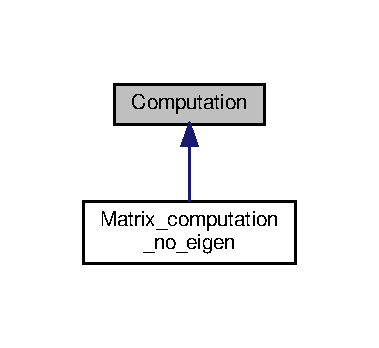
\includegraphics[width=182pt]{classComputation__inherit__graph}
\end{center}
\end{figure}
\subsection*{Public Member Functions}
\begin{DoxyCompactItemize}
\item 
virtual void \hyperlink{classComputation_a1b2d101b74dadde0624f837a62c051c6}{compute} ()=0\hypertarget{classComputation_a1b2d101b74dadde0624f837a62c051c6}{}\label{classComputation_a1b2d101b74dadde0624f837a62c051c6}

\begin{DoxyCompactList}\small\item\em Interface to some computation to perform in the real time thread. \end{DoxyCompactList}\end{DoxyCompactItemize}


\subsection{Detailed Description}
Abstract interface for some different thread computation. 

The documentation for this class was generated from the following file\+:\begin{DoxyCompactItemize}
\item 
src/bin/\hyperlink{realtime__test_8cpp}{realtime\+\_\+test.\+cpp}\end{DoxyCompactItemize}

\hypertarget{classConfiguration}{}\section{Configuration Class Reference}
\label{classConfiguration}\index{Configuration@{Configuration}}


\hyperlink{classConfiguration}{Configuration} of the test thread.  


\subsection*{Public Attributes}
\begin{DoxyCompactItemize}
\item 
int \hyperlink{classConfiguration_a7d5f2036941892a92f343c50a1606b4d}{mode}\hypertarget{classConfiguration_a7d5f2036941892a92f343c50a1606b4d}{}\label{classConfiguration_a7d5f2036941892a92f343c50a1606b4d}

\begin{DoxyCompactList}\small\item\em mode of the thread \end{DoxyCompactList}\item 
double \hyperlink{classConfiguration_ac6f09be53002bfb5404a241b3ce5486e}{frequency}\hypertarget{classConfiguration_ac6f09be53002bfb5404a241b3ce5486e}{}\label{classConfiguration_ac6f09be53002bfb5404a241b3ce5486e}

\begin{DoxyCompactList}\small\item\em thread frequency \end{DoxyCompactList}\item 
double \hyperlink{classConfiguration_abeda8dee257cb5a21afa2d1f6fab758c}{switch\+\_\+frequency}\hypertarget{classConfiguration_abeda8dee257cb5a21afa2d1f6fab758c}{}\label{classConfiguration_abeda8dee257cb5a21afa2d1f6fab758c}

\begin{DoxyCompactList}\small\item\em bound on the achieved frequency \end{DoxyCompactList}\end{DoxyCompactItemize}


\subsection{Detailed Description}
\hyperlink{classConfiguration}{Configuration} of the test thread. 

The documentation for this class was generated from the following file\+:\begin{DoxyCompactItemize}
\item 
src/bin/\hyperlink{realtime__test_8cpp}{realtime\+\_\+test.\+cpp}\end{DoxyCompactItemize}

\hypertarget{classreal__time__tools_1_1FrequencyManager}{}\section{real\+\_\+time\+\_\+tools\+:\+:Frequency\+Manager Class Reference}
\label{classreal__time__tools_1_1FrequencyManager}\index{real\+\_\+time\+\_\+tools\+::\+Frequency\+Manager@{real\+\_\+time\+\_\+tools\+::\+Frequency\+Manager}}


Class to have threads / loops running at a desired frequency.  




{\ttfamily \#include $<$frequency\+\_\+manager.\+hpp$>$}

\subsection*{Public Member Functions}
\begin{DoxyCompactItemize}
\item 
{\bfseries Frequency\+Manager} (double frequency)\hypertarget{classreal__time__tools_1_1FrequencyManager_a218f8a2651b453a89daa2968e2610032}{}\label{classreal__time__tools_1_1FrequencyManager_a218f8a2651b453a89daa2968e2610032}

\item 
bool \hyperlink{classreal__time__tools_1_1FrequencyManager_a3496f77c75f5ac8013b9f62345595e80}{wait} ()
\begin{DoxyCompactList}\small\item\em waits for the time such that successive calls to wait will result in wait being called at the desired frequency \end{DoxyCompactList}\end{DoxyCompactItemize}
\subsection*{Private Attributes}
\begin{DoxyCompactItemize}
\item 
double {\bfseries period\+\_\+ms\+\_\+}\hypertarget{classreal__time__tools_1_1FrequencyManager_ad32d927286a10fff1aefbb46d44748e1}{}\label{classreal__time__tools_1_1FrequencyManager_ad32d927286a10fff1aefbb46d44748e1}

\item 
double {\bfseries previous\+\_\+time\+\_\+ms\+\_\+}\hypertarget{classreal__time__tools_1_1FrequencyManager_a42fa6ff042ee8de87d85b8875bd2723f}{}\label{classreal__time__tools_1_1FrequencyManager_a42fa6ff042ee8de87d85b8875bd2723f}

\end{DoxyCompactItemize}


\subsection{Detailed Description}
Class to have threads / loops running at a desired frequency. 

\subsection{Member Function Documentation}
\index{real\+\_\+time\+\_\+tools\+::\+Frequency\+Manager@{real\+\_\+time\+\_\+tools\+::\+Frequency\+Manager}!wait@{wait}}
\index{wait@{wait}!real\+\_\+time\+\_\+tools\+::\+Frequency\+Manager@{real\+\_\+time\+\_\+tools\+::\+Frequency\+Manager}}
\subsubsection[{\texorpdfstring{wait()}{wait()}}]{\setlength{\rightskip}{0pt plus 5cm}bool real\+\_\+time\+\_\+tools\+::\+Frequency\+Manager\+::wait (
\begin{DoxyParamCaption}
{}
\end{DoxyParamCaption}
)}\hypertarget{classreal__time__tools_1_1FrequencyManager_a3496f77c75f5ac8013b9f62345595e80}{}\label{classreal__time__tools_1_1FrequencyManager_a3496f77c75f5ac8013b9f62345595e80}


waits for the time such that successive calls to wait will result in wait being called at the desired frequency 

\begin{DoxyReturn}{Returns}
true if the desired frequency could be enforced 
\end{DoxyReturn}


The documentation for this class was generated from the following files\+:\begin{DoxyCompactItemize}
\item 
include/real\+\_\+time\+\_\+tools/\hyperlink{frequency__manager_8hpp}{frequency\+\_\+manager.\+hpp}\item 
src/frequency\+\_\+manager.\+cpp\end{DoxyCompactItemize}

\hypertarget{classMatrix__computation__no__eigen}{}\section{Matrix\+\_\+computation\+\_\+no\+\_\+eigen Class Reference}
\label{classMatrix__computation__no__eigen}\index{Matrix\+\_\+computation\+\_\+no\+\_\+eigen@{Matrix\+\_\+computation\+\_\+no\+\_\+eigen}}


Some specific computation based on matrix multiplication.  




Inheritance diagram for Matrix\+\_\+computation\+\_\+no\+\_\+eigen\+:
\nopagebreak
\begin{figure}[H]
\begin{center}
\leavevmode
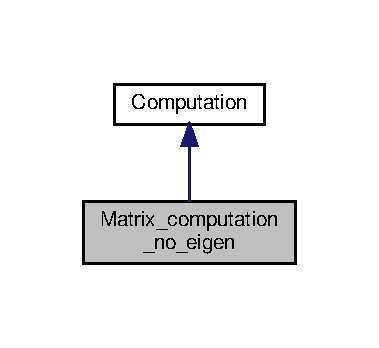
\includegraphics[width=182pt]{classMatrix__computation__no__eigen__inherit__graph}
\end{center}
\end{figure}


Collaboration diagram for Matrix\+\_\+computation\+\_\+no\+\_\+eigen\+:
\nopagebreak
\begin{figure}[H]
\begin{center}
\leavevmode
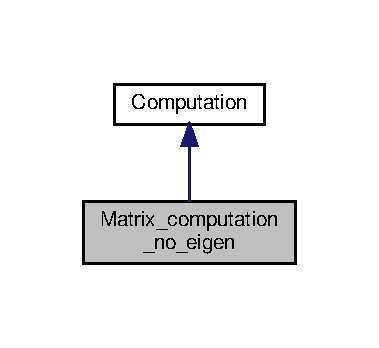
\includegraphics[width=182pt]{classMatrix__computation__no__eigen__coll__graph}
\end{center}
\end{figure}
\subsection*{Public Member Functions}
\begin{DoxyCompactItemize}
\item 
\hyperlink{classMatrix__computation__no__eigen_af70d9fcfdc0c9a9b755a9261211dce8a}{Matrix\+\_\+computation\+\_\+no\+\_\+eigen} (int \hyperlink{classMatrix__computation__no__eigen_a1f73cf9e7670c6a78a64cb8977f2dcc6}{size})
\begin{DoxyCompactList}\small\item\em Construct a new \hyperlink{classMatrix__computation__no__eigen}{Matrix\+\_\+computation\+\_\+no\+\_\+eigen} object. \end{DoxyCompactList}\item 
\mbox{\Hypertarget{classMatrix__computation__no__eigen_a47f33ea53cf14f1c6b86218203c8af26}\label{classMatrix__computation__no__eigen_a47f33ea53cf14f1c6b86218203c8af26}} 
\hyperlink{classMatrix__computation__no__eigen_a47f33ea53cf14f1c6b86218203c8af26}{$\sim$\+Matrix\+\_\+computation\+\_\+no\+\_\+eigen} ()
\begin{DoxyCompactList}\small\item\em class destructor \end{DoxyCompactList}\item 
double \hyperlink{classMatrix__computation__no__eigen_a588b833136c503e9726d7276f358f117}{compute} (int i, int j)
\begin{DoxyCompactList}\small\item\em Compute one element of the matrix multiplication. \end{DoxyCompactList}\item 
void \hyperlink{classMatrix__computation__no__eigen_a7fbc5e6986b2f630e8356e4d276aa03e}{compute} ()
\begin{DoxyCompactList}\small\item\em compute the matrix multiplication. \end{DoxyCompactList}\end{DoxyCompactItemize}
\subsection*{Private Attributes}
\begin{DoxyCompactItemize}
\item 
int \hyperlink{classMatrix__computation__no__eigen_a1f73cf9e7670c6a78a64cb8977f2dcc6}{size}
\begin{DoxyCompactList}\small\item\em The size of the matrices. \end{DoxyCompactList}\item 
double $\ast$$\ast$ \hyperlink{classMatrix__computation__no__eigen_a66d9dde3f7fc191c8be8b23a1c7764e2}{m1}
\begin{DoxyCompactList}\small\item\em The first matrix. \end{DoxyCompactList}\item 
double $\ast$$\ast$ \hyperlink{classMatrix__computation__no__eigen_a4cda5f8f06be2a85621b1ce1eca7cded}{m2}
\begin{DoxyCompactList}\small\item\em The second matrix. \end{DoxyCompactList}\item 
double $\ast$$\ast$ \hyperlink{classMatrix__computation__no__eigen_a54b2738e77b3282368ac2c7fd184d2a3}{m3}
\begin{DoxyCompactList}\small\item\em The multiplication of the first 2 matrices. \end{DoxyCompactList}\end{DoxyCompactItemize}


\subsection{Detailed Description}
Some specific computation based on matrix multiplication. 

\subsection{Constructor \& Destructor Documentation}
\mbox{\Hypertarget{classMatrix__computation__no__eigen_af70d9fcfdc0c9a9b755a9261211dce8a}\label{classMatrix__computation__no__eigen_af70d9fcfdc0c9a9b755a9261211dce8a}} 
\index{Matrix\+\_\+computation\+\_\+no\+\_\+eigen@{Matrix\+\_\+computation\+\_\+no\+\_\+eigen}!Matrix\+\_\+computation\+\_\+no\+\_\+eigen@{Matrix\+\_\+computation\+\_\+no\+\_\+eigen}}
\index{Matrix\+\_\+computation\+\_\+no\+\_\+eigen@{Matrix\+\_\+computation\+\_\+no\+\_\+eigen}!Matrix\+\_\+computation\+\_\+no\+\_\+eigen@{Matrix\+\_\+computation\+\_\+no\+\_\+eigen}}
\subsubsection{\texorpdfstring{Matrix\+\_\+computation\+\_\+no\+\_\+eigen()}{Matrix\_computation\_no\_eigen()}}
{\footnotesize\ttfamily Matrix\+\_\+computation\+\_\+no\+\_\+eigen\+::\+Matrix\+\_\+computation\+\_\+no\+\_\+eigen (\begin{DoxyParamCaption}\item[{int}]{size }\end{DoxyParamCaption})\hspace{0.3cm}{\ttfamily [inline]}}



Construct a new \hyperlink{classMatrix__computation__no__eigen}{Matrix\+\_\+computation\+\_\+no\+\_\+eigen} object. 


\begin{DoxyParams}{Parameters}
{\em size} & of the matrices \\
\hline
\end{DoxyParams}


\subsection{Member Function Documentation}
\mbox{\Hypertarget{classMatrix__computation__no__eigen_a588b833136c503e9726d7276f358f117}\label{classMatrix__computation__no__eigen_a588b833136c503e9726d7276f358f117}} 
\index{Matrix\+\_\+computation\+\_\+no\+\_\+eigen@{Matrix\+\_\+computation\+\_\+no\+\_\+eigen}!compute@{compute}}
\index{compute@{compute}!Matrix\+\_\+computation\+\_\+no\+\_\+eigen@{Matrix\+\_\+computation\+\_\+no\+\_\+eigen}}
\subsubsection{\texorpdfstring{compute()}{compute()}\hspace{0.1cm}{\footnotesize\ttfamily [1/2]}}
{\footnotesize\ttfamily double Matrix\+\_\+computation\+\_\+no\+\_\+eigen\+::compute (\begin{DoxyParamCaption}\item[{int}]{i,  }\item[{int}]{j }\end{DoxyParamCaption})\hspace{0.3cm}{\ttfamily [inline]}}



Compute one element of the matrix multiplication. 


\begin{DoxyParams}{Parameters}
{\em i} & $ i^th $ row \\
\hline
{\em j} & $ j^th $ column \\
\hline
\end{DoxyParams}
\begin{DoxyReturn}{Returns}
double result of the multiplication 
\end{DoxyReturn}
\mbox{\Hypertarget{classMatrix__computation__no__eigen_a7fbc5e6986b2f630e8356e4d276aa03e}\label{classMatrix__computation__no__eigen_a7fbc5e6986b2f630e8356e4d276aa03e}} 
\index{Matrix\+\_\+computation\+\_\+no\+\_\+eigen@{Matrix\+\_\+computation\+\_\+no\+\_\+eigen}!compute@{compute}}
\index{compute@{compute}!Matrix\+\_\+computation\+\_\+no\+\_\+eigen@{Matrix\+\_\+computation\+\_\+no\+\_\+eigen}}
\subsubsection{\texorpdfstring{compute()}{compute()}\hspace{0.1cm}{\footnotesize\ttfamily [2/2]}}
{\footnotesize\ttfamily void Matrix\+\_\+computation\+\_\+no\+\_\+eigen\+::compute (\begin{DoxyParamCaption}{ }\end{DoxyParamCaption})\hspace{0.3cm}{\ttfamily [inline]}, {\ttfamily [virtual]}}



compute the matrix multiplication. 



Implements \hyperlink{classComputation_a1b2d101b74dadde0624f837a62c051c6}{Computation}.



\subsection{Member Data Documentation}
\mbox{\Hypertarget{classMatrix__computation__no__eigen_a66d9dde3f7fc191c8be8b23a1c7764e2}\label{classMatrix__computation__no__eigen_a66d9dde3f7fc191c8be8b23a1c7764e2}} 
\index{Matrix\+\_\+computation\+\_\+no\+\_\+eigen@{Matrix\+\_\+computation\+\_\+no\+\_\+eigen}!m1@{m1}}
\index{m1@{m1}!Matrix\+\_\+computation\+\_\+no\+\_\+eigen@{Matrix\+\_\+computation\+\_\+no\+\_\+eigen}}
\subsubsection{\texorpdfstring{m1}{m1}}
{\footnotesize\ttfamily double$\ast$$\ast$ Matrix\+\_\+computation\+\_\+no\+\_\+eigen\+::m1\hspace{0.3cm}{\ttfamily [private]}}



The first matrix. 

\mbox{\Hypertarget{classMatrix__computation__no__eigen_a4cda5f8f06be2a85621b1ce1eca7cded}\label{classMatrix__computation__no__eigen_a4cda5f8f06be2a85621b1ce1eca7cded}} 
\index{Matrix\+\_\+computation\+\_\+no\+\_\+eigen@{Matrix\+\_\+computation\+\_\+no\+\_\+eigen}!m2@{m2}}
\index{m2@{m2}!Matrix\+\_\+computation\+\_\+no\+\_\+eigen@{Matrix\+\_\+computation\+\_\+no\+\_\+eigen}}
\subsubsection{\texorpdfstring{m2}{m2}}
{\footnotesize\ttfamily double$\ast$$\ast$ Matrix\+\_\+computation\+\_\+no\+\_\+eigen\+::m2\hspace{0.3cm}{\ttfamily [private]}}



The second matrix. 

\mbox{\Hypertarget{classMatrix__computation__no__eigen_a54b2738e77b3282368ac2c7fd184d2a3}\label{classMatrix__computation__no__eigen_a54b2738e77b3282368ac2c7fd184d2a3}} 
\index{Matrix\+\_\+computation\+\_\+no\+\_\+eigen@{Matrix\+\_\+computation\+\_\+no\+\_\+eigen}!m3@{m3}}
\index{m3@{m3}!Matrix\+\_\+computation\+\_\+no\+\_\+eigen@{Matrix\+\_\+computation\+\_\+no\+\_\+eigen}}
\subsubsection{\texorpdfstring{m3}{m3}}
{\footnotesize\ttfamily double$\ast$$\ast$ Matrix\+\_\+computation\+\_\+no\+\_\+eigen\+::m3\hspace{0.3cm}{\ttfamily [private]}}



The multiplication of the first 2 matrices. 

\mbox{\Hypertarget{classMatrix__computation__no__eigen_a1f73cf9e7670c6a78a64cb8977f2dcc6}\label{classMatrix__computation__no__eigen_a1f73cf9e7670c6a78a64cb8977f2dcc6}} 
\index{Matrix\+\_\+computation\+\_\+no\+\_\+eigen@{Matrix\+\_\+computation\+\_\+no\+\_\+eigen}!size@{size}}
\index{size@{size}!Matrix\+\_\+computation\+\_\+no\+\_\+eigen@{Matrix\+\_\+computation\+\_\+no\+\_\+eigen}}
\subsubsection{\texorpdfstring{size}{size}}
{\footnotesize\ttfamily int Matrix\+\_\+computation\+\_\+no\+\_\+eigen\+::size\hspace{0.3cm}{\ttfamily [private]}}



The size of the matrices. 



The documentation for this class was generated from the following file\+:\begin{DoxyCompactItemize}
\item 
src/bin/\hyperlink{realtime__test_8cpp}{realtime\+\_\+test.\+cpp}\end{DoxyCompactItemize}

\hypertarget{classreal__time__tools_1_1PortConfig}{}\section{real\+\_\+time\+\_\+tools\+:\+:Port\+Config Class Reference}
\label{classreal__time__tools_1_1PortConfig}\index{real\+\_\+time\+\_\+tools\+::\+Port\+Config@{real\+\_\+time\+\_\+tools\+::\+Port\+Config}}


Simple config class that encapsulate the port parameters for a U\+SB port.  




{\ttfamily \#include $<$usb\+\_\+stream.\+hpp$>$}

\subsection*{Public Types}
\begin{DoxyCompactItemize}
\item 
\mbox{\Hypertarget{classreal__time__tools_1_1PortConfig_a62bbab15705e2d5a9bc17115222f7c07}\label{classreal__time__tools_1_1PortConfig_a62bbab15705e2d5a9bc17115222f7c07}} 
enum \hyperlink{classreal__time__tools_1_1PortConfig_a62bbab15705e2d5a9bc17115222f7c07}{Stop\+Bits} \{ {\bfseries one} = 1, 
{\bfseries two} = 2
 \}\begin{DoxyCompactList}\small\item\em This is if one wants 1 or 2 stop bits. \end{DoxyCompactList}
\item 
\mbox{\Hypertarget{classreal__time__tools_1_1PortConfig_a11e818aa26cd0a941ff00b9ccd4d2131}\label{classreal__time__tools_1_1PortConfig_a11e818aa26cd0a941ff00b9ccd4d2131}} 
enum \hyperlink{classreal__time__tools_1_1PortConfig_a11e818aa26cd0a941ff00b9ccd4d2131}{Data\+Bits} \{ {\bfseries cs7} = 0, 
{\bfseries cs8} = 1
 \}\begin{DoxyCompactList}\small\item\em This correspond to the number of data bits echanged. \end{DoxyCompactList}
\end{DoxyCompactItemize}
\subsection*{Public Member Functions}
\begin{DoxyCompactItemize}
\item 
int \hyperlink{classreal__time__tools_1_1PortConfig_a9dc2941d278825ecc20a5f260a7fb076}{get\+\_\+bauderate} ()
\begin{DoxyCompactList}\small\item\em Get the \+\_\+bauderate object. \end{DoxyCompactList}\end{DoxyCompactItemize}
\subsection*{Public Attributes}
\begin{DoxyCompactItemize}
\item 
bool \hyperlink{classreal__time__tools_1_1PortConfig_ad89a20459faf7718a63ea8c00ddc5e34}{rts\+\_\+cts\+\_\+enabled\+\_\+}
\begin{DoxyCompactList}\small\item\em Enabling/\+Disabling rts cts. \end{DoxyCompactList}\item 
\mbox{\Hypertarget{classreal__time__tools_1_1PortConfig_afdc811c6c73ada4b21dab246bf086506}\label{classreal__time__tools_1_1PortConfig_afdc811c6c73ada4b21dab246bf086506}} 
bool \hyperlink{classreal__time__tools_1_1PortConfig_afdc811c6c73ada4b21dab246bf086506}{parity\+\_\+}
\begin{DoxyCompactList}\small\item\em Use or not a parity bit. \end{DoxyCompactList}\item 
\hyperlink{classreal__time__tools_1_1PortConfig_a62bbab15705e2d5a9bc17115222f7c07}{Stop\+Bits} \hyperlink{classreal__time__tools_1_1PortConfig_a3303d793237edbfa0b3c28f3f01c3837}{stop\+\_\+bits\+\_\+}
\begin{DoxyCompactList}\small\item\em Defines the choice of the stop bits. \end{DoxyCompactList}\item 
\mbox{\Hypertarget{classreal__time__tools_1_1PortConfig_a6c1dbeb3cf3c772c9c1b4df71b8befd6}\label{classreal__time__tools_1_1PortConfig_a6c1dbeb3cf3c772c9c1b4df71b8befd6}} 
bool \hyperlink{classreal__time__tools_1_1PortConfig_a6c1dbeb3cf3c772c9c1b4df71b8befd6}{prepare\+\_\+size\+\_\+definition\+\_\+}
\begin{DoxyCompactList}\small\item\em Defines if the port should prepare the size definition. \end{DoxyCompactList}\item 
\hyperlink{classreal__time__tools_1_1PortConfig_a11e818aa26cd0a941ff00b9ccd4d2131}{Data\+Bits} \hyperlink{classreal__time__tools_1_1PortConfig_af80f9991e3811392385208a9baf9c6fd}{data\+\_\+bits\+\_\+}
\begin{DoxyCompactList}\small\item\em Defines the number of bits echanged. \end{DoxyCompactList}\item 
int \hyperlink{classreal__time__tools_1_1PortConfig_aa0be2d74f3ac70e9f43d36fc0c70901a}{baude\+\_\+rate\+\_\+}
\begin{DoxyCompactList}\small\item\em Defines the Baude\+Rate to be used. \end{DoxyCompactList}\end{DoxyCompactItemize}


\subsection{Detailed Description}
Simple config class that encapsulate the port parameters for a U\+SB port. 

This should cover enough paramter to setup the U\+SB port for the imu\+\_\+3\+D\+M\+\_\+\+G\+X3\+\_\+25, imu\+\_\+3\+D\+M\+\_\+\+G\+X3\+\_\+45 and the imu\+\_\+3\+D\+M\+\_\+\+G\+X5 in xenomai, rt\+\_\+preempt and ubuntu (potentially Mac\+OS\+: non posix). \begin{Desc}
\item[Examples\+: ]\par
\hyperlink{demo_usb_stream_imu_3DM_GX3_25_8cpp-example}{demo\+\_\+usb\+\_\+stream\+\_\+imu\+\_\+3\+D\+M\+\_\+\+G\+X3\+\_\+25.\+cpp}.\end{Desc}


\subsection{Member Function Documentation}
\mbox{\Hypertarget{classreal__time__tools_1_1PortConfig_a9dc2941d278825ecc20a5f260a7fb076}\label{classreal__time__tools_1_1PortConfig_a9dc2941d278825ecc20a5f260a7fb076}} 
\index{real\+\_\+time\+\_\+tools\+::\+Port\+Config@{real\+\_\+time\+\_\+tools\+::\+Port\+Config}!get\+\_\+bauderate@{get\+\_\+bauderate}}
\index{get\+\_\+bauderate@{get\+\_\+bauderate}!real\+\_\+time\+\_\+tools\+::\+Port\+Config@{real\+\_\+time\+\_\+tools\+::\+Port\+Config}}
\subsubsection{\texorpdfstring{get\+\_\+bauderate()}{get\_bauderate()}}
{\footnotesize\ttfamily int real\+\_\+time\+\_\+tools\+::\+Port\+Config\+::get\+\_\+bauderate (\begin{DoxyParamCaption}{ }\end{DoxyParamCaption})}



Get the \+\_\+bauderate object. 

\begin{DoxyReturn}{Returns}
int 
\end{DoxyReturn}


\subsection{Member Data Documentation}
\mbox{\Hypertarget{classreal__time__tools_1_1PortConfig_aa0be2d74f3ac70e9f43d36fc0c70901a}\label{classreal__time__tools_1_1PortConfig_aa0be2d74f3ac70e9f43d36fc0c70901a}} 
\index{real\+\_\+time\+\_\+tools\+::\+Port\+Config@{real\+\_\+time\+\_\+tools\+::\+Port\+Config}!baude\+\_\+rate\+\_\+@{baude\+\_\+rate\+\_\+}}
\index{baude\+\_\+rate\+\_\+@{baude\+\_\+rate\+\_\+}!real\+\_\+time\+\_\+tools\+::\+Port\+Config@{real\+\_\+time\+\_\+tools\+::\+Port\+Config}}
\subsubsection{\texorpdfstring{baude\+\_\+rate\+\_\+}{baude\_rate\_}}
{\footnotesize\ttfamily int real\+\_\+time\+\_\+tools\+::\+Port\+Config\+::baude\+\_\+rate\+\_\+}



Defines the Baude\+Rate to be used. 

(see enum Baude\+Rate) \begin{Desc}
\item[Examples\+: ]\par
\hyperlink{demo_usb_stream_imu_3DM_GX3_25_8cpp-example}{demo\+\_\+usb\+\_\+stream\+\_\+imu\+\_\+3\+D\+M\+\_\+\+G\+X3\+\_\+25.\+cpp}.\end{Desc}
\mbox{\Hypertarget{classreal__time__tools_1_1PortConfig_af80f9991e3811392385208a9baf9c6fd}\label{classreal__time__tools_1_1PortConfig_af80f9991e3811392385208a9baf9c6fd}} 
\index{real\+\_\+time\+\_\+tools\+::\+Port\+Config@{real\+\_\+time\+\_\+tools\+::\+Port\+Config}!data\+\_\+bits\+\_\+@{data\+\_\+bits\+\_\+}}
\index{data\+\_\+bits\+\_\+@{data\+\_\+bits\+\_\+}!real\+\_\+time\+\_\+tools\+::\+Port\+Config@{real\+\_\+time\+\_\+tools\+::\+Port\+Config}}
\subsubsection{\texorpdfstring{data\+\_\+bits\+\_\+}{data\_bits\_}}
{\footnotesize\ttfamily \hyperlink{classreal__time__tools_1_1PortConfig_a11e818aa26cd0a941ff00b9ccd4d2131}{Data\+Bits} real\+\_\+time\+\_\+tools\+::\+Port\+Config\+::data\+\_\+bits\+\_\+}



Defines the number of bits echanged. 

(see enum Data\+Bits) \begin{Desc}
\item[Examples\+: ]\par
\hyperlink{demo_usb_stream_imu_3DM_GX3_25_8cpp-example}{demo\+\_\+usb\+\_\+stream\+\_\+imu\+\_\+3\+D\+M\+\_\+\+G\+X3\+\_\+25.\+cpp}.\end{Desc}
\mbox{\Hypertarget{classreal__time__tools_1_1PortConfig_ad89a20459faf7718a63ea8c00ddc5e34}\label{classreal__time__tools_1_1PortConfig_ad89a20459faf7718a63ea8c00ddc5e34}} 
\index{real\+\_\+time\+\_\+tools\+::\+Port\+Config@{real\+\_\+time\+\_\+tools\+::\+Port\+Config}!rts\+\_\+cts\+\_\+enabled\+\_\+@{rts\+\_\+cts\+\_\+enabled\+\_\+}}
\index{rts\+\_\+cts\+\_\+enabled\+\_\+@{rts\+\_\+cts\+\_\+enabled\+\_\+}!real\+\_\+time\+\_\+tools\+::\+Port\+Config@{real\+\_\+time\+\_\+tools\+::\+Port\+Config}}
\subsubsection{\texorpdfstring{rts\+\_\+cts\+\_\+enabled\+\_\+}{rts\_cts\_enabled\_}}
{\footnotesize\ttfamily bool real\+\_\+time\+\_\+tools\+::\+Port\+Config\+::rts\+\_\+cts\+\_\+enabled\+\_\+}



Enabling/\+Disabling rts cts. 

T\+O\+DO\+: look for what is rts cts \begin{Desc}
\item[Examples\+: ]\par
\hyperlink{demo_usb_stream_imu_3DM_GX3_25_8cpp-example}{demo\+\_\+usb\+\_\+stream\+\_\+imu\+\_\+3\+D\+M\+\_\+\+G\+X3\+\_\+25.\+cpp}.\end{Desc}
\mbox{\Hypertarget{classreal__time__tools_1_1PortConfig_a3303d793237edbfa0b3c28f3f01c3837}\label{classreal__time__tools_1_1PortConfig_a3303d793237edbfa0b3c28f3f01c3837}} 
\index{real\+\_\+time\+\_\+tools\+::\+Port\+Config@{real\+\_\+time\+\_\+tools\+::\+Port\+Config}!stop\+\_\+bits\+\_\+@{stop\+\_\+bits\+\_\+}}
\index{stop\+\_\+bits\+\_\+@{stop\+\_\+bits\+\_\+}!real\+\_\+time\+\_\+tools\+::\+Port\+Config@{real\+\_\+time\+\_\+tools\+::\+Port\+Config}}
\subsubsection{\texorpdfstring{stop\+\_\+bits\+\_\+}{stop\_bits\_}}
{\footnotesize\ttfamily \hyperlink{classreal__time__tools_1_1PortConfig_a62bbab15705e2d5a9bc17115222f7c07}{Stop\+Bits} real\+\_\+time\+\_\+tools\+::\+Port\+Config\+::stop\+\_\+bits\+\_\+}



Defines the choice of the stop bits. 

(see enum Stop\+Bits) \begin{Desc}
\item[Examples\+: ]\par
\hyperlink{demo_usb_stream_imu_3DM_GX3_25_8cpp-example}{demo\+\_\+usb\+\_\+stream\+\_\+imu\+\_\+3\+D\+M\+\_\+\+G\+X3\+\_\+25.\+cpp}.\end{Desc}


The documentation for this class was generated from the following file\+:\begin{DoxyCompactItemize}
\item 
include/real\+\_\+time\+\_\+tools/usb\+\_\+stream.\+hpp\end{DoxyCompactItemize}

\hypertarget{classreal__time__tools_1_1RealTimeCheck}{}\section{real\+\_\+time\+\_\+tools\+:\+:Real\+Time\+Check Class Reference}
\label{classreal__time__tools_1_1RealTimeCheck}\index{real\+\_\+time\+\_\+tools\+::\+Real\+Time\+Check@{real\+\_\+time\+\_\+tools\+::\+Real\+Time\+Check}}


super simple class for checking if thread ever lost realtime.  




{\ttfamily \#include $<$realtime\+\_\+check.\+hpp$>$}

\subsection*{Public Member Functions}
\begin{DoxyCompactItemize}
\item 
\hyperlink{classreal__time__tools_1_1RealTimeCheck_a2f26472092432e628167f89a3a19e27e}{Real\+Time\+Check} (double \hyperlink{classreal__time__tools_1_1RealTimeCheck_a126c13a50d06703c515b35f87c3e867c}{target\+\_\+frequency}, double \hyperlink{classreal__time__tools_1_1RealTimeCheck_a235895032a789539a8ba957caac621ec}{switch\+\_\+frequency})
\begin{DoxyCompactList}\small\item\em Construct a new \hyperlink{classreal__time__tools_1_1RealTimeCheck}{Real\+Time\+Check} object. \end{DoxyCompactList}\item 
void \hyperlink{classreal__time__tools_1_1RealTimeCheck_a83fdf97352d36aa20e482d7dfae442d5}{tick} ()
\item 
bool \hyperlink{classreal__time__tools_1_1RealTimeCheck_af4fcff0b49162ff802192c2e4832568a}{was\+\_\+realtime\+\_\+lost} () const 
\item 
bool \hyperlink{classreal__time__tools_1_1RealTimeCheck_a4d9614b08d2b4bf7162e14c473b7d491}{get\+\_\+statistics} (int \&\hyperlink{classreal__time__tools_1_1RealTimeCheck_ae2acb20d9f1e49cc35eb5505d63201aa}{ticks}, int \&\hyperlink{classreal__time__tools_1_1RealTimeCheck_acc235579eeb245f043fd188790540fa9}{switchs}, double \&\hyperlink{classreal__time__tools_1_1RealTimeCheck_a126c13a50d06703c515b35f87c3e867c}{target\+\_\+frequency}, double \&\hyperlink{classreal__time__tools_1_1RealTimeCheck_a235895032a789539a8ba957caac621ec}{switch\+\_\+frequency}, double \&\hyperlink{classreal__time__tools_1_1RealTimeCheck_a3ffb6de7e7c01a7248c2293e29b98011}{average\+\_\+frequency}, double \&\hyperlink{classreal__time__tools_1_1RealTimeCheck_a935b4c6b8ebf569e6510d47376f8499f}{current\+\_\+frequency}, double \&\hyperlink{classreal__time__tools_1_1RealTimeCheck_a3605c41d8c5c616879fa9af469860470}{worse\+\_\+frequency})
\item 
double \hyperlink{classreal__time__tools_1_1RealTimeCheck_a2b891d59055829fab442ba4c382778e3}{get\+\_\+average\+\_\+frequency} ()
\item 
double \hyperlink{classreal__time__tools_1_1RealTimeCheck_a1cd5c3fb05a46970361064348c57197d}{get\+\_\+current\+\_\+frequency} () const 
\item 
void \hyperlink{classreal__time__tools_1_1RealTimeCheck_a9c9c68da79843098085204095286a143}{print} ()
\end{DoxyCompactItemize}
\subsection*{Private Attributes}
\begin{DoxyCompactItemize}
\item 
bool \hyperlink{classreal__time__tools_1_1RealTimeCheck_a21b5703a3c61b09955d94d06a3562667}{started}
\item 
std\+::chrono\+::high\+\_\+resolution\+\_\+clock\+::time\+\_\+point \hyperlink{classreal__time__tools_1_1RealTimeCheck_a969600ce8ecc4ec48bbf59e8d669749e}{start\+\_\+time}
\item 
std\+::chrono\+::high\+\_\+resolution\+\_\+clock\+::time\+\_\+point \hyperlink{classreal__time__tools_1_1RealTimeCheck_a3e200c0376362dcc9a7db7d77a124931}{last\+\_\+tick}
\item 
double \hyperlink{classreal__time__tools_1_1RealTimeCheck_a126c13a50d06703c515b35f87c3e867c}{target\+\_\+frequency}
\item 
double \hyperlink{classreal__time__tools_1_1RealTimeCheck_ab6a059be584e4a92254002d35713d0df}{epsilon}
\item 
uint \hyperlink{classreal__time__tools_1_1RealTimeCheck_ae2acb20d9f1e49cc35eb5505d63201aa}{ticks}
\item 
uint \hyperlink{classreal__time__tools_1_1RealTimeCheck_acc235579eeb245f043fd188790540fa9}{switchs}
\item 
double \hyperlink{classreal__time__tools_1_1RealTimeCheck_a3ffb6de7e7c01a7248c2293e29b98011}{average\+\_\+frequency}
\item 
double \hyperlink{classreal__time__tools_1_1RealTimeCheck_a3605c41d8c5c616879fa9af469860470}{worse\+\_\+frequency}
\item 
double \hyperlink{classreal__time__tools_1_1RealTimeCheck_a235895032a789539a8ba957caac621ec}{switch\+\_\+frequency}
\item 
double \hyperlink{classreal__time__tools_1_1RealTimeCheck_a935b4c6b8ebf569e6510d47376f8499f}{current\+\_\+frequency}
\item 
std\+::mutex \hyperlink{classreal__time__tools_1_1RealTimeCheck_a3a7cc4ef87fac5e4052a3240aced88d1}{mutex}
\end{DoxyCompactItemize}


\subsection{Detailed Description}
super simple class for checking if thread ever lost realtime. 

simply measure frequency between two calls to the tick function. \begin{Desc}
\item[Examples\+: ]\par
\hyperlink{demo_realtime_check_8cpp-example}{demo\+\_\+realtime\+\_\+check.\+cpp}, \hyperlink{demo_realtime_strict_check_8cpp-example}{demo\+\_\+realtime\+\_\+strict\+\_\+check.\+cpp}, and \hyperlink{demo_spinner_8cpp-example}{demo\+\_\+spinner.\+cpp}.\end{Desc}


\subsection{Constructor \& Destructor Documentation}
\index{real\+\_\+time\+\_\+tools\+::\+Real\+Time\+Check@{real\+\_\+time\+\_\+tools\+::\+Real\+Time\+Check}!Real\+Time\+Check@{Real\+Time\+Check}}
\index{Real\+Time\+Check@{Real\+Time\+Check}!real\+\_\+time\+\_\+tools\+::\+Real\+Time\+Check@{real\+\_\+time\+\_\+tools\+::\+Real\+Time\+Check}}
\subsubsection[{\texorpdfstring{Real\+Time\+Check(double target\+\_\+frequency, double switch\+\_\+frequency)}{RealTimeCheck(double target_frequency, double switch_frequency)}}]{\setlength{\rightskip}{0pt plus 5cm}real\+\_\+time\+\_\+tools\+::\+Real\+Time\+Check\+::\+Real\+Time\+Check (
\begin{DoxyParamCaption}
\item[{double}]{target\+\_\+frequency, }
\item[{double}]{switch\+\_\+frequency}
\end{DoxyParamCaption}
)}\hypertarget{classreal__time__tools_1_1RealTimeCheck_a2f26472092432e628167f89a3a19e27e}{}\label{classreal__time__tools_1_1RealTimeCheck_a2f26472092432e628167f89a3a19e27e}


Construct a new \hyperlink{classreal__time__tools_1_1RealTimeCheck}{Real\+Time\+Check} object. 


\begin{DoxyParams}{Parameters}
{\em target\+\_\+frequency} & is the loop frequency. \\
\hline
{\em switch\+\_\+frequency} & is the admissible frequency. \\
\hline
\end{DoxyParams}


\subsection{Member Function Documentation}
\index{real\+\_\+time\+\_\+tools\+::\+Real\+Time\+Check@{real\+\_\+time\+\_\+tools\+::\+Real\+Time\+Check}!get\+\_\+average\+\_\+frequency@{get\+\_\+average\+\_\+frequency}}
\index{get\+\_\+average\+\_\+frequency@{get\+\_\+average\+\_\+frequency}!real\+\_\+time\+\_\+tools\+::\+Real\+Time\+Check@{real\+\_\+time\+\_\+tools\+::\+Real\+Time\+Check}}
\subsubsection[{\texorpdfstring{get\+\_\+average\+\_\+frequency()}{get_average_frequency()}}]{\setlength{\rightskip}{0pt plus 5cm}double real\+\_\+time\+\_\+tools\+::\+Real\+Time\+Check\+::get\+\_\+average\+\_\+frequency (
\begin{DoxyParamCaption}
{}
\end{DoxyParamCaption}
)}\hypertarget{classreal__time__tools_1_1RealTimeCheck_a2b891d59055829fab442ba4c382778e3}{}\label{classreal__time__tools_1_1RealTimeCheck_a2b891d59055829fab442ba4c382778e3}
return the averaged observed frequency if statistics are available, -\/1 otherwise (false is returned is tick has never been called or if ticks reached maximum integer value). \index{real\+\_\+time\+\_\+tools\+::\+Real\+Time\+Check@{real\+\_\+time\+\_\+tools\+::\+Real\+Time\+Check}!get\+\_\+current\+\_\+frequency@{get\+\_\+current\+\_\+frequency}}
\index{get\+\_\+current\+\_\+frequency@{get\+\_\+current\+\_\+frequency}!real\+\_\+time\+\_\+tools\+::\+Real\+Time\+Check@{real\+\_\+time\+\_\+tools\+::\+Real\+Time\+Check}}
\subsubsection[{\texorpdfstring{get\+\_\+current\+\_\+frequency() const }{get_current_frequency() const }}]{\setlength{\rightskip}{0pt plus 5cm}double real\+\_\+time\+\_\+tools\+::\+Real\+Time\+Check\+::get\+\_\+current\+\_\+frequency (
\begin{DoxyParamCaption}
{}
\end{DoxyParamCaption}
) const}\hypertarget{classreal__time__tools_1_1RealTimeCheck_a1cd5c3fb05a46970361064348c57197d}{}\label{classreal__time__tools_1_1RealTimeCheck_a1cd5c3fb05a46970361064348c57197d}
returns observed frequency after last call to tick \index{real\+\_\+time\+\_\+tools\+::\+Real\+Time\+Check@{real\+\_\+time\+\_\+tools\+::\+Real\+Time\+Check}!get\+\_\+statistics@{get\+\_\+statistics}}
\index{get\+\_\+statistics@{get\+\_\+statistics}!real\+\_\+time\+\_\+tools\+::\+Real\+Time\+Check@{real\+\_\+time\+\_\+tools\+::\+Real\+Time\+Check}}
\subsubsection[{\texorpdfstring{get\+\_\+statistics(int \&ticks, int \&switchs, double \&target\+\_\+frequency, double \&switch\+\_\+frequency, double \&average\+\_\+frequency, double \&current\+\_\+frequency, double \&worse\+\_\+frequency)}{get_statistics(int &ticks, int &switchs, double &target_frequency, double &switch_frequency, double &average_frequency, double &current_frequency, double &worse_frequency)}}]{\setlength{\rightskip}{0pt plus 5cm}bool real\+\_\+time\+\_\+tools\+::\+Real\+Time\+Check\+::get\+\_\+statistics (
\begin{DoxyParamCaption}
\item[{int \&}]{ticks, }
\item[{int \&}]{switchs, }
\item[{double \&}]{target\+\_\+frequency, }
\item[{double \&}]{switch\+\_\+frequency, }
\item[{double \&}]{average\+\_\+frequency, }
\item[{double \&}]{current\+\_\+frequency, }
\item[{double \&}]{worse\+\_\+frequency}
\end{DoxyParamCaption}
)}\hypertarget{classreal__time__tools_1_1RealTimeCheck_a4d9614b08d2b4bf7162e14c473b7d491}{}\label{classreal__time__tools_1_1RealTimeCheck_a4d9614b08d2b4bf7162e14c473b7d491}
return true if statistics are available, false otherwise (false is returned is tick has never been called or if ticks reached maximum integer value) switchs in the number of time realtime was lost. \index{real\+\_\+time\+\_\+tools\+::\+Real\+Time\+Check@{real\+\_\+time\+\_\+tools\+::\+Real\+Time\+Check}!print@{print}}
\index{print@{print}!real\+\_\+time\+\_\+tools\+::\+Real\+Time\+Check@{real\+\_\+time\+\_\+tools\+::\+Real\+Time\+Check}}
\subsubsection[{\texorpdfstring{print()}{print()}}]{\setlength{\rightskip}{0pt plus 5cm}void real\+\_\+time\+\_\+tools\+::\+Real\+Time\+Check\+::print (
\begin{DoxyParamCaption}
{}
\end{DoxyParamCaption}
)}\hypertarget{classreal__time__tools_1_1RealTimeCheck_a9c9c68da79843098085204095286a143}{}\label{classreal__time__tools_1_1RealTimeCheck_a9c9c68da79843098085204095286a143}
Display the results of the frequency measurement. \begin{Desc}
\item[Examples\+: ]\par
\hyperlink{demo_realtime_check_8cpp-example}{demo\+\_\+realtime\+\_\+check.\+cpp}, \hyperlink{demo_realtime_strict_check_8cpp-example}{demo\+\_\+realtime\+\_\+strict\+\_\+check.\+cpp}, and \hyperlink{demo_spinner_8cpp-example}{demo\+\_\+spinner.\+cpp}.\end{Desc}
\index{real\+\_\+time\+\_\+tools\+::\+Real\+Time\+Check@{real\+\_\+time\+\_\+tools\+::\+Real\+Time\+Check}!tick@{tick}}
\index{tick@{tick}!real\+\_\+time\+\_\+tools\+::\+Real\+Time\+Check@{real\+\_\+time\+\_\+tools\+::\+Real\+Time\+Check}}
\subsubsection[{\texorpdfstring{tick()}{tick()}}]{\setlength{\rightskip}{0pt plus 5cm}void real\+\_\+time\+\_\+tools\+::\+Real\+Time\+Check\+::tick (
\begin{DoxyParamCaption}
{}
\end{DoxyParamCaption}
)}\hypertarget{classreal__time__tools_1_1RealTimeCheck_a83fdf97352d36aa20e482d7dfae442d5}{}\label{classreal__time__tools_1_1RealTimeCheck_a83fdf97352d36aa20e482d7dfae442d5}
inform the instance of this class that an iteration passed \begin{Desc}
\item[Examples\+: ]\par
\hyperlink{demo_realtime_check_8cpp-example}{demo\+\_\+realtime\+\_\+check.\+cpp}, \hyperlink{demo_realtime_strict_check_8cpp-example}{demo\+\_\+realtime\+\_\+strict\+\_\+check.\+cpp}, and \hyperlink{demo_spinner_8cpp-example}{demo\+\_\+spinner.\+cpp}.\end{Desc}
\index{real\+\_\+time\+\_\+tools\+::\+Real\+Time\+Check@{real\+\_\+time\+\_\+tools\+::\+Real\+Time\+Check}!was\+\_\+realtime\+\_\+lost@{was\+\_\+realtime\+\_\+lost}}
\index{was\+\_\+realtime\+\_\+lost@{was\+\_\+realtime\+\_\+lost}!real\+\_\+time\+\_\+tools\+::\+Real\+Time\+Check@{real\+\_\+time\+\_\+tools\+::\+Real\+Time\+Check}}
\subsubsection[{\texorpdfstring{was\+\_\+realtime\+\_\+lost() const }{was_realtime_lost() const }}]{\setlength{\rightskip}{0pt plus 5cm}bool real\+\_\+time\+\_\+tools\+::\+Real\+Time\+Check\+::was\+\_\+realtime\+\_\+lost (
\begin{DoxyParamCaption}
{}
\end{DoxyParamCaption}
) const}\hypertarget{classreal__time__tools_1_1RealTimeCheck_af4fcff0b49162ff802192c2e4832568a}{}\label{classreal__time__tools_1_1RealTimeCheck_af4fcff0b49162ff802192c2e4832568a}
true if realtime was lost at least once (frequency between two ticks was below target frequencies) 

\subsection{Member Data Documentation}
\index{real\+\_\+time\+\_\+tools\+::\+Real\+Time\+Check@{real\+\_\+time\+\_\+tools\+::\+Real\+Time\+Check}!average\+\_\+frequency@{average\+\_\+frequency}}
\index{average\+\_\+frequency@{average\+\_\+frequency}!real\+\_\+time\+\_\+tools\+::\+Real\+Time\+Check@{real\+\_\+time\+\_\+tools\+::\+Real\+Time\+Check}}
\subsubsection[{\texorpdfstring{average\+\_\+frequency}{average_frequency}}]{\setlength{\rightskip}{0pt plus 5cm}double real\+\_\+time\+\_\+tools\+::\+Real\+Time\+Check\+::average\+\_\+frequency\hspace{0.3cm}{\ttfamily [private]}}\hypertarget{classreal__time__tools_1_1RealTimeCheck_a3ffb6de7e7c01a7248c2293e29b98011}{}\label{classreal__time__tools_1_1RealTimeCheck_a3ffb6de7e7c01a7248c2293e29b98011}
average frequency \index{real\+\_\+time\+\_\+tools\+::\+Real\+Time\+Check@{real\+\_\+time\+\_\+tools\+::\+Real\+Time\+Check}!current\+\_\+frequency@{current\+\_\+frequency}}
\index{current\+\_\+frequency@{current\+\_\+frequency}!real\+\_\+time\+\_\+tools\+::\+Real\+Time\+Check@{real\+\_\+time\+\_\+tools\+::\+Real\+Time\+Check}}
\subsubsection[{\texorpdfstring{current\+\_\+frequency}{current_frequency}}]{\setlength{\rightskip}{0pt plus 5cm}double real\+\_\+time\+\_\+tools\+::\+Real\+Time\+Check\+::current\+\_\+frequency\hspace{0.3cm}{\ttfamily [private]}}\hypertarget{classreal__time__tools_1_1RealTimeCheck_a935b4c6b8ebf569e6510d47376f8499f}{}\label{classreal__time__tools_1_1RealTimeCheck_a935b4c6b8ebf569e6510d47376f8499f}
latest frequency that was measured \index{real\+\_\+time\+\_\+tools\+::\+Real\+Time\+Check@{real\+\_\+time\+\_\+tools\+::\+Real\+Time\+Check}!epsilon@{epsilon}}
\index{epsilon@{epsilon}!real\+\_\+time\+\_\+tools\+::\+Real\+Time\+Check@{real\+\_\+time\+\_\+tools\+::\+Real\+Time\+Check}}
\subsubsection[{\texorpdfstring{epsilon}{epsilon}}]{\setlength{\rightskip}{0pt plus 5cm}double real\+\_\+time\+\_\+tools\+::\+Real\+Time\+Check\+::epsilon\hspace{0.3cm}{\ttfamily [private]}}\hypertarget{classreal__time__tools_1_1RealTimeCheck_ab6a059be584e4a92254002d35713d0df}{}\label{classreal__time__tools_1_1RealTimeCheck_ab6a059be584e4a92254002d35713d0df}
small quantity \index{real\+\_\+time\+\_\+tools\+::\+Real\+Time\+Check@{real\+\_\+time\+\_\+tools\+::\+Real\+Time\+Check}!last\+\_\+tick@{last\+\_\+tick}}
\index{last\+\_\+tick@{last\+\_\+tick}!real\+\_\+time\+\_\+tools\+::\+Real\+Time\+Check@{real\+\_\+time\+\_\+tools\+::\+Real\+Time\+Check}}
\subsubsection[{\texorpdfstring{last\+\_\+tick}{last_tick}}]{\setlength{\rightskip}{0pt plus 5cm}std\+::chrono\+::high\+\_\+resolution\+\_\+clock\+::time\+\_\+point real\+\_\+time\+\_\+tools\+::\+Real\+Time\+Check\+::last\+\_\+tick\hspace{0.3cm}{\ttfamily [private]}}\hypertarget{classreal__time__tools_1_1RealTimeCheck_a3e200c0376362dcc9a7db7d77a124931}{}\label{classreal__time__tools_1_1RealTimeCheck_a3e200c0376362dcc9a7db7d77a124931}
last time system was ticked \index{real\+\_\+time\+\_\+tools\+::\+Real\+Time\+Check@{real\+\_\+time\+\_\+tools\+::\+Real\+Time\+Check}!mutex@{mutex}}
\index{mutex@{mutex}!real\+\_\+time\+\_\+tools\+::\+Real\+Time\+Check@{real\+\_\+time\+\_\+tools\+::\+Real\+Time\+Check}}
\subsubsection[{\texorpdfstring{mutex}{mutex}}]{\setlength{\rightskip}{0pt plus 5cm}std\+::mutex real\+\_\+time\+\_\+tools\+::\+Real\+Time\+Check\+::mutex\hspace{0.3cm}{\ttfamily [private]}}\hypertarget{classreal__time__tools_1_1RealTimeCheck_a3a7cc4ef87fac5e4052a3240aced88d1}{}\label{classreal__time__tools_1_1RealTimeCheck_a3a7cc4ef87fac5e4052a3240aced88d1}
multithreading safety \index{real\+\_\+time\+\_\+tools\+::\+Real\+Time\+Check@{real\+\_\+time\+\_\+tools\+::\+Real\+Time\+Check}!start\+\_\+time@{start\+\_\+time}}
\index{start\+\_\+time@{start\+\_\+time}!real\+\_\+time\+\_\+tools\+::\+Real\+Time\+Check@{real\+\_\+time\+\_\+tools\+::\+Real\+Time\+Check}}
\subsubsection[{\texorpdfstring{start\+\_\+time}{start_time}}]{\setlength{\rightskip}{0pt plus 5cm}std\+::chrono\+::high\+\_\+resolution\+\_\+clock\+::time\+\_\+point real\+\_\+time\+\_\+tools\+::\+Real\+Time\+Check\+::start\+\_\+time\hspace{0.3cm}{\ttfamily [private]}}\hypertarget{classreal__time__tools_1_1RealTimeCheck_a969600ce8ecc4ec48bbf59e8d669749e}{}\label{classreal__time__tools_1_1RealTimeCheck_a969600ce8ecc4ec48bbf59e8d669749e}
time at which tick was called first \index{real\+\_\+time\+\_\+tools\+::\+Real\+Time\+Check@{real\+\_\+time\+\_\+tools\+::\+Real\+Time\+Check}!started@{started}}
\index{started@{started}!real\+\_\+time\+\_\+tools\+::\+Real\+Time\+Check@{real\+\_\+time\+\_\+tools\+::\+Real\+Time\+Check}}
\subsubsection[{\texorpdfstring{started}{started}}]{\setlength{\rightskip}{0pt plus 5cm}bool real\+\_\+time\+\_\+tools\+::\+Real\+Time\+Check\+::started\hspace{0.3cm}{\ttfamily [private]}}\hypertarget{classreal__time__tools_1_1RealTimeCheck_a21b5703a3c61b09955d94d06a3562667}{}\label{classreal__time__tools_1_1RealTimeCheck_a21b5703a3c61b09955d94d06a3562667}
true if tick has been called once \index{real\+\_\+time\+\_\+tools\+::\+Real\+Time\+Check@{real\+\_\+time\+\_\+tools\+::\+Real\+Time\+Check}!switch\+\_\+frequency@{switch\+\_\+frequency}}
\index{switch\+\_\+frequency@{switch\+\_\+frequency}!real\+\_\+time\+\_\+tools\+::\+Real\+Time\+Check@{real\+\_\+time\+\_\+tools\+::\+Real\+Time\+Check}}
\subsubsection[{\texorpdfstring{switch\+\_\+frequency}{switch_frequency}}]{\setlength{\rightskip}{0pt plus 5cm}double real\+\_\+time\+\_\+tools\+::\+Real\+Time\+Check\+::switch\+\_\+frequency\hspace{0.3cm}{\ttfamily [private]}}\hypertarget{classreal__time__tools_1_1RealTimeCheck_a235895032a789539a8ba957caac621ec}{}\label{classreal__time__tools_1_1RealTimeCheck_a235895032a789539a8ba957caac621ec}
nb of switches will increase by 1 each time measured frequency below this value \index{real\+\_\+time\+\_\+tools\+::\+Real\+Time\+Check@{real\+\_\+time\+\_\+tools\+::\+Real\+Time\+Check}!switchs@{switchs}}
\index{switchs@{switchs}!real\+\_\+time\+\_\+tools\+::\+Real\+Time\+Check@{real\+\_\+time\+\_\+tools\+::\+Real\+Time\+Check}}
\subsubsection[{\texorpdfstring{switchs}{switchs}}]{\setlength{\rightskip}{0pt plus 5cm}uint real\+\_\+time\+\_\+tools\+::\+Real\+Time\+Check\+::switchs\hspace{0.3cm}{\ttfamily [private]}}\hypertarget{classreal__time__tools_1_1RealTimeCheck_acc235579eeb245f043fd188790540fa9}{}\label{classreal__time__tools_1_1RealTimeCheck_acc235579eeb245f043fd188790540fa9}
number of time realtime was lost (target frequency not respected between two ticks) \index{real\+\_\+time\+\_\+tools\+::\+Real\+Time\+Check@{real\+\_\+time\+\_\+tools\+::\+Real\+Time\+Check}!target\+\_\+frequency@{target\+\_\+frequency}}
\index{target\+\_\+frequency@{target\+\_\+frequency}!real\+\_\+time\+\_\+tools\+::\+Real\+Time\+Check@{real\+\_\+time\+\_\+tools\+::\+Real\+Time\+Check}}
\subsubsection[{\texorpdfstring{target\+\_\+frequency}{target_frequency}}]{\setlength{\rightskip}{0pt plus 5cm}double real\+\_\+time\+\_\+tools\+::\+Real\+Time\+Check\+::target\+\_\+frequency\hspace{0.3cm}{\ttfamily [private]}}\hypertarget{classreal__time__tools_1_1RealTimeCheck_a126c13a50d06703c515b35f87c3e867c}{}\label{classreal__time__tools_1_1RealTimeCheck_a126c13a50d06703c515b35f87c3e867c}
frequency at which ticks are expected \index{real\+\_\+time\+\_\+tools\+::\+Real\+Time\+Check@{real\+\_\+time\+\_\+tools\+::\+Real\+Time\+Check}!ticks@{ticks}}
\index{ticks@{ticks}!real\+\_\+time\+\_\+tools\+::\+Real\+Time\+Check@{real\+\_\+time\+\_\+tools\+::\+Real\+Time\+Check}}
\subsubsection[{\texorpdfstring{ticks}{ticks}}]{\setlength{\rightskip}{0pt plus 5cm}uint real\+\_\+time\+\_\+tools\+::\+Real\+Time\+Check\+::ticks\hspace{0.3cm}{\ttfamily [private]}}\hypertarget{classreal__time__tools_1_1RealTimeCheck_ae2acb20d9f1e49cc35eb5505d63201aa}{}\label{classreal__time__tools_1_1RealTimeCheck_ae2acb20d9f1e49cc35eb5505d63201aa}
number of iterations \index{real\+\_\+time\+\_\+tools\+::\+Real\+Time\+Check@{real\+\_\+time\+\_\+tools\+::\+Real\+Time\+Check}!worse\+\_\+frequency@{worse\+\_\+frequency}}
\index{worse\+\_\+frequency@{worse\+\_\+frequency}!real\+\_\+time\+\_\+tools\+::\+Real\+Time\+Check@{real\+\_\+time\+\_\+tools\+::\+Real\+Time\+Check}}
\subsubsection[{\texorpdfstring{worse\+\_\+frequency}{worse_frequency}}]{\setlength{\rightskip}{0pt plus 5cm}double real\+\_\+time\+\_\+tools\+::\+Real\+Time\+Check\+::worse\+\_\+frequency\hspace{0.3cm}{\ttfamily [private]}}\hypertarget{classreal__time__tools_1_1RealTimeCheck_a3605c41d8c5c616879fa9af469860470}{}\label{classreal__time__tools_1_1RealTimeCheck_a3605c41d8c5c616879fa9af469860470}
worse frequency ever experienced 

The documentation for this class was generated from the following files\+:\begin{DoxyCompactItemize}
\item 
include/real\+\_\+time\+\_\+tools/\hyperlink{realtime__check_8hpp}{realtime\+\_\+check.\+hpp}\item 
src/\hyperlink{realtime__check_8cpp}{realtime\+\_\+check.\+cpp}\end{DoxyCompactItemize}

\hypertarget{classreal__time__tools_1_1RealTimeMutex}{}\section{real\+\_\+time\+\_\+tools\+:\+:Real\+Time\+Mutex Class Reference}
\label{classreal__time__tools_1_1RealTimeMutex}\index{real\+\_\+time\+\_\+tools\+::\+Real\+Time\+Mutex@{real\+\_\+time\+\_\+tools\+::\+Real\+Time\+Mutex}}


This class uses the real-\/time A\+PI of xenomai and posix to implement mutexes.  




{\ttfamily \#include $<$mutex.\+hpp$>$}

\subsection*{Public Member Functions}
\begin{DoxyCompactItemize}
\item 
\mbox{\Hypertarget{classreal__time__tools_1_1RealTimeMutex_aef1777e27f3f2802ebcc7cb6db101df0}\label{classreal__time__tools_1_1RealTimeMutex_aef1777e27f3f2802ebcc7cb6db101df0}} 
\hyperlink{classreal__time__tools_1_1RealTimeMutex_aef1777e27f3f2802ebcc7cb6db101df0}{Real\+Time\+Mutex} (std\+::string mutex\+\_\+id=\char`\"{}\char`\"{})
\begin{DoxyCompactList}\small\item\em Construct a new \hyperlink{classreal__time__tools_1_1RealTimeMutex}{Real\+Time\+Mutex} object. \end{DoxyCompactList}\item 
\mbox{\Hypertarget{classreal__time__tools_1_1RealTimeMutex_a86c9ab73fb02cf4a954735d56f4f23ed}\label{classreal__time__tools_1_1RealTimeMutex_a86c9ab73fb02cf4a954735d56f4f23ed}} 
\hyperlink{classreal__time__tools_1_1RealTimeMutex_a86c9ab73fb02cf4a954735d56f4f23ed}{$\sim$\+Real\+Time\+Mutex} ()
\begin{DoxyCompactList}\small\item\em Destroy the \hyperlink{classreal__time__tools_1_1RealTimeMutex}{Real\+Time\+Mutex} object. \end{DoxyCompactList}\item 
\mbox{\Hypertarget{classreal__time__tools_1_1RealTimeMutex_a38d84501c3929f8dbb3c884299cfcb9c}\label{classreal__time__tools_1_1RealTimeMutex_a38d84501c3929f8dbb3c884299cfcb9c}} 
void \hyperlink{classreal__time__tools_1_1RealTimeMutex_a38d84501c3929f8dbb3c884299cfcb9c}{lock} ()
\begin{DoxyCompactList}\small\item\em lock the mutex. \end{DoxyCompactList}\item 
\mbox{\Hypertarget{classreal__time__tools_1_1RealTimeMutex_a9b85b1aa898c22197dffc3958e0ec60c}\label{classreal__time__tools_1_1RealTimeMutex_a9b85b1aa898c22197dffc3958e0ec60c}} 
void \hyperlink{classreal__time__tools_1_1RealTimeMutex_a9b85b1aa898c22197dffc3958e0ec60c}{unlock} ()
\begin{DoxyCompactList}\small\item\em unlock the mutex \end{DoxyCompactList}\end{DoxyCompactItemize}
\subsection*{Private Attributes}
\begin{DoxyCompactItemize}
\item 
\mbox{\Hypertarget{classreal__time__tools_1_1RealTimeMutex_a21e60b2fffe69eba625590fa3201404b}\label{classreal__time__tools_1_1RealTimeMutex_a21e60b2fffe69eba625590fa3201404b}} 
\hyperlink{mutex_8hpp_a1ddc3c11c7ede92bbf52bafb61009ba2}{Real\+Time\+Mutex\+\_\+t} \hyperlink{classreal__time__tools_1_1RealTimeMutex_a21e60b2fffe69eba625590fa3201404b}{mutex\+\_\+}
\begin{DoxyCompactList}\small\item\em This is the object which type chenge according to the OS this code is compiled. \end{DoxyCompactList}\item 
\mbox{\Hypertarget{classreal__time__tools_1_1RealTimeMutex_a42edb13b07a983e48d9348bb20465962}\label{classreal__time__tools_1_1RealTimeMutex_a42edb13b07a983e48d9348bb20465962}} 
std\+::string \hyperlink{classreal__time__tools_1_1RealTimeMutex_a42edb13b07a983e48d9348bb20465962}{mutex\+\_\+id\+\_\+}
\begin{DoxyCompactList}\small\item\em Save the mutex id internally. \end{DoxyCompactList}\end{DoxyCompactItemize}


\subsection{Detailed Description}
This class uses the real-\/time A\+PI of xenomai and posix to implement mutexes. 

The documentation for this class was generated from the following file\+:\begin{DoxyCompactItemize}
\item 
include/real\+\_\+time\+\_\+tools/\hyperlink{mutex_8hpp}{mutex.\+hpp}\end{DoxyCompactItemize}

\hypertarget{classreal__time__tools_1_1RealTimeThread}{}\section{real\+\_\+time\+\_\+tools\+:\+:Real\+Time\+Thread Class Reference}
\label{classreal__time__tools_1_1RealTimeThread}\index{real\+\_\+time\+\_\+tools\+::\+Real\+Time\+Thread@{real\+\_\+time\+\_\+tools\+::\+Real\+Time\+Thread}}


This class allows you to spawn thread.  




{\ttfamily \#include $<$thread.\+hpp$>$}



Collaboration diagram for real\+\_\+time\+\_\+tools\+:\+:Real\+Time\+Thread\+:
\nopagebreak
\begin{figure}[H]
\begin{center}
\leavevmode
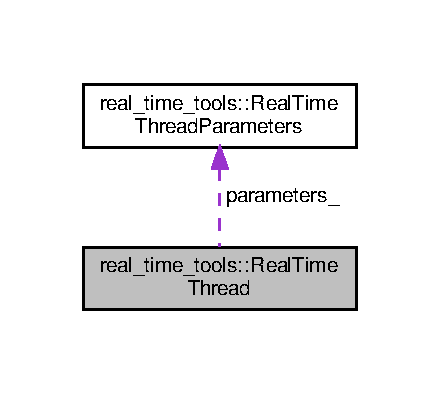
\includegraphics[width=211pt]{classreal__time__tools_1_1RealTimeThread__coll__graph}
\end{center}
\end{figure}
\subsection*{Public Member Functions}
\begin{DoxyCompactItemize}
\item 
\hyperlink{classreal__time__tools_1_1RealTimeThread_aca6224b9cbe75e3a85b281e0de096b64}{Real\+Time\+Thread} ()\hypertarget{classreal__time__tools_1_1RealTimeThread_aca6224b9cbe75e3a85b281e0de096b64}{}\label{classreal__time__tools_1_1RealTimeThread_aca6224b9cbe75e3a85b281e0de096b64}

\begin{DoxyCompactList}\small\item\em Construct a new Thread\+Info object. \end{DoxyCompactList}\item 
\hyperlink{classreal__time__tools_1_1RealTimeThread_a5d2cba4b8f65bdbf36edc0bcc589e45e}{Real\+Time\+Thread} (const \hyperlink{classreal__time__tools_1_1RealTimeThread}{real\+\_\+time\+\_\+tools\+::\+Real\+Time\+Thread} \&other)=delete\hypertarget{classreal__time__tools_1_1RealTimeThread_a5d2cba4b8f65bdbf36edc0bcc589e45e}{}\label{classreal__time__tools_1_1RealTimeThread_a5d2cba4b8f65bdbf36edc0bcc589e45e}

\begin{DoxyCompactList}\small\item\em We do not allow copies of this object. \end{DoxyCompactList}\item 
\hyperlink{classreal__time__tools_1_1RealTimeThread_a8e94b07c6ff51d50b1861887fbd1f69f}{$\sim$\+Real\+Time\+Thread} ()\hypertarget{classreal__time__tools_1_1RealTimeThread_a8e94b07c6ff51d50b1861887fbd1f69f}{}\label{classreal__time__tools_1_1RealTimeThread_a8e94b07c6ff51d50b1861887fbd1f69f}

\begin{DoxyCompactList}\small\item\em Destroy the \hyperlink{classreal__time__tools_1_1RealTimeThread}{Real\+Time\+Thread} object. \end{DoxyCompactList}\item 
int \hyperlink{classreal__time__tools_1_1RealTimeThread_a232e3955fee6e80c3a7ded68f165414b}{create\+\_\+realtime\+\_\+thread} (void $\ast$($\ast$\hyperlink{realtime__test_8cpp_a54b1343eb90254009bd964c44996761b}{thread\+\_\+function})(void $\ast$), void $\ast$args=nullptr)
\begin{DoxyCompactList}\small\item\em create\+\_\+realtime\+\_\+thread spawns a real time thread if the OS allows it. \end{DoxyCompactList}\item 
int \hyperlink{classreal__time__tools_1_1RealTimeThread_a2f455db9fd80b81e5e69cd22e8529979}{join} ()
\begin{DoxyCompactList}\small\item\em join join the real time thread \end{DoxyCompactList}\item 
void \hyperlink{classreal__time__tools_1_1RealTimeThread_a704b245872cc7bc49e01181f09732535}{block\+\_\+memory} ()
\begin{DoxyCompactList}\small\item\em block\+\_\+memory block the current and futur memory pages. \end{DoxyCompactList}\end{DoxyCompactItemize}
\subsection*{Public Attributes}
\begin{DoxyCompactItemize}
\item 
\hyperlink{classreal__time__tools_1_1RealTimeThreadParameters}{Real\+Time\+Thread\+Parameters} \hyperlink{classreal__time__tools_1_1RealTimeThread_aa15b5633e76ea6b4c31cd74b3968686a}{parameters\+\_\+}\hypertarget{classreal__time__tools_1_1RealTimeThread_aa15b5633e76ea6b4c31cd74b3968686a}{}\label{classreal__time__tools_1_1RealTimeThread_aa15b5633e76ea6b4c31cd74b3968686a}

\begin{DoxyCompactList}\small\item\em Paramter of the real time thread. \end{DoxyCompactList}\end{DoxyCompactItemize}


\subsection{Detailed Description}
This class allows you to spawn thread. 

Its parameter are defined above. \begin{Desc}
\item[Examples\+: ]\par
\hyperlink{demo_realtime_check_8cpp-example}{demo\+\_\+realtime\+\_\+check.\+cpp}, \hyperlink{demo_realtime_strict_check_8cpp-example}{demo\+\_\+realtime\+\_\+strict\+\_\+check.\+cpp}, \hyperlink{demo_spinner_8cpp-example}{demo\+\_\+spinner.\+cpp}, and \hyperlink{demo_timing_8cpp-example}{demo\+\_\+timing.\+cpp}.\end{Desc}


\subsection{Member Function Documentation}
\index{real\+\_\+time\+\_\+tools\+::\+Real\+Time\+Thread@{real\+\_\+time\+\_\+tools\+::\+Real\+Time\+Thread}!block\+\_\+memory@{block\+\_\+memory}}
\index{block\+\_\+memory@{block\+\_\+memory}!real\+\_\+time\+\_\+tools\+::\+Real\+Time\+Thread@{real\+\_\+time\+\_\+tools\+::\+Real\+Time\+Thread}}
\subsubsection[{\texorpdfstring{block\+\_\+memory()}{block_memory()}}]{\setlength{\rightskip}{0pt plus 5cm}void real\+\_\+time\+\_\+tools\+::\+Real\+Time\+Thread\+::block\+\_\+memory (
\begin{DoxyParamCaption}
{}
\end{DoxyParamCaption}
)}\hypertarget{classreal__time__tools_1_1RealTimeThread_a704b245872cc7bc49e01181f09732535}{}\label{classreal__time__tools_1_1RealTimeThread_a704b245872cc7bc49e01181f09732535}


block\+\_\+memory block the current and futur memory pages. 

see \href{https://wiki.linuxfoundation.org/realtime/documentation/howto/applications/memory#memory-locking}{\tt https\+://wiki.\+linuxfoundation.\+org/realtime/documentation/howto/applications/memory\#memory-\/locking} for further explanation. \index{real\+\_\+time\+\_\+tools\+::\+Real\+Time\+Thread@{real\+\_\+time\+\_\+tools\+::\+Real\+Time\+Thread}!create\+\_\+realtime\+\_\+thread@{create\+\_\+realtime\+\_\+thread}}
\index{create\+\_\+realtime\+\_\+thread@{create\+\_\+realtime\+\_\+thread}!real\+\_\+time\+\_\+tools\+::\+Real\+Time\+Thread@{real\+\_\+time\+\_\+tools\+::\+Real\+Time\+Thread}}
\subsubsection[{\texorpdfstring{create\+\_\+realtime\+\_\+thread(void $\ast$($\ast$thread\+\_\+function)(void $\ast$), void $\ast$args=nullptr)}{create_realtime_thread(void *(*thread_function)(void *), void *args=nullptr)}}]{\setlength{\rightskip}{0pt plus 5cm}int real\+\_\+time\+\_\+tools\+::\+Real\+Time\+Thread\+::create\+\_\+realtime\+\_\+thread (
\begin{DoxyParamCaption}
\item[{void $\ast$($\ast$)(void $\ast$)}]{thread\+\_\+function, }
\item[{void $\ast$}]{args = {\ttfamily nullptr}}
\end{DoxyParamCaption}
)}\hypertarget{classreal__time__tools_1_1RealTimeThread_a232e3955fee6e80c3a7ded68f165414b}{}\label{classreal__time__tools_1_1RealTimeThread_a232e3955fee6e80c3a7ded68f165414b}


create\+\_\+realtime\+\_\+thread spawns a real time thread if the OS allows it. 


\begin{DoxyParams}[1]{Parameters}
\mbox{\tt in}  & {\em thread\+\_\+function} & the executing function for the thread. \\
\hline
\mbox{\tt in}  & {\em args} & arguments to be passed to the thread. \\
\hline
\end{DoxyParams}
\begin{DoxyReturn}{Returns}
the error code. 
\end{DoxyReturn}
\begin{Desc}
\item[Examples\+: ]\par
\hyperlink{demo_realtime_check_8cpp-example}{demo\+\_\+realtime\+\_\+check.\+cpp}, \hyperlink{demo_realtime_strict_check_8cpp-example}{demo\+\_\+realtime\+\_\+strict\+\_\+check.\+cpp}, \hyperlink{demo_spinner_8cpp-example}{demo\+\_\+spinner.\+cpp}, and \hyperlink{demo_timing_8cpp-example}{demo\+\_\+timing.\+cpp}.\end{Desc}
\index{real\+\_\+time\+\_\+tools\+::\+Real\+Time\+Thread@{real\+\_\+time\+\_\+tools\+::\+Real\+Time\+Thread}!join@{join}}
\index{join@{join}!real\+\_\+time\+\_\+tools\+::\+Real\+Time\+Thread@{real\+\_\+time\+\_\+tools\+::\+Real\+Time\+Thread}}
\subsubsection[{\texorpdfstring{join()}{join()}}]{\setlength{\rightskip}{0pt plus 5cm}int real\+\_\+time\+\_\+tools\+::\+Real\+Time\+Thread\+::join (
\begin{DoxyParamCaption}
{}
\end{DoxyParamCaption}
)}\hypertarget{classreal__time__tools_1_1RealTimeThread_a2f455db9fd80b81e5e69cd22e8529979}{}\label{classreal__time__tools_1_1RealTimeThread_a2f455db9fd80b81e5e69cd22e8529979}


join join the real time thread 

\begin{DoxyReturn}{Returns}
the error code. 
\end{DoxyReturn}
\begin{Desc}
\item[Examples\+: ]\par
\hyperlink{demo_realtime_check_8cpp-example}{demo\+\_\+realtime\+\_\+check.\+cpp}, \hyperlink{demo_realtime_strict_check_8cpp-example}{demo\+\_\+realtime\+\_\+strict\+\_\+check.\+cpp}, \hyperlink{demo_spinner_8cpp-example}{demo\+\_\+spinner.\+cpp}, and \hyperlink{demo_timing_8cpp-example}{demo\+\_\+timing.\+cpp}.\end{Desc}


The documentation for this class was generated from the following file\+:\begin{DoxyCompactItemize}
\item 
include/real\+\_\+time\+\_\+tools/\hyperlink{thread_8hpp}{thread.\+hpp}\end{DoxyCompactItemize}

\hypertarget{classreal__time__tools_1_1RealTimeThreadParameters}{}\section{real\+\_\+time\+\_\+tools\+:\+:Real\+Time\+Thread\+Parameters Class Reference}
\label{classreal__time__tools_1_1RealTimeThreadParameters}\index{real\+\_\+time\+\_\+tools\+::\+Real\+Time\+Thread\+Parameters@{real\+\_\+time\+\_\+tools\+::\+Real\+Time\+Thread\+Parameters}}


This class is a data structure allowing the user to share configurations among threads.  




{\ttfamily \#include $<$thread.\+hpp$>$}

\subsection*{Public Member Functions}
\begin{DoxyCompactItemize}
\item 
\hyperlink{classreal__time__tools_1_1RealTimeThreadParameters_a3c23c4f6a5b8ac991072e247f536fcd8}{Real\+Time\+Thread\+Parameters} ()\hypertarget{classreal__time__tools_1_1RealTimeThreadParameters_a3c23c4f6a5b8ac991072e247f536fcd8}{}\label{classreal__time__tools_1_1RealTimeThreadParameters_a3c23c4f6a5b8ac991072e247f536fcd8}

\begin{DoxyCompactList}\small\item\em Construct a new \hyperlink{classreal__time__tools_1_1RealTimeThreadParameters}{Real\+Time\+Thread\+Parameters} object. \end{DoxyCompactList}\item 
\hyperlink{classreal__time__tools_1_1RealTimeThreadParameters_a9b6720cd9e0da2ad81e22e337a76d7ea}{$\sim$\+Real\+Time\+Thread\+Parameters} ()\hypertarget{classreal__time__tools_1_1RealTimeThreadParameters_a9b6720cd9e0da2ad81e22e337a76d7ea}{}\label{classreal__time__tools_1_1RealTimeThreadParameters_a9b6720cd9e0da2ad81e22e337a76d7ea}

\begin{DoxyCompactList}\small\item\em Destroy the \hyperlink{classreal__time__tools_1_1RealTimeThreadParameters}{Real\+Time\+Thread\+Parameters} object. \end{DoxyCompactList}\end{DoxyCompactItemize}
\subsection*{Public Attributes}
\begin{DoxyCompactItemize}
\item 
std\+::string \hyperlink{classreal__time__tools_1_1RealTimeThreadParameters_a9db02f30ad6b4d6cfa3ca49dbd63e0f4}{keyword\+\_\+}\hypertarget{classreal__time__tools_1_1RealTimeThreadParameters_a9db02f30ad6b4d6cfa3ca49dbd63e0f4}{}\label{classreal__time__tools_1_1RealTimeThreadParameters_a9db02f30ad6b4d6cfa3ca49dbd63e0f4}

\begin{DoxyCompactList}\small\item\em Used in xenomai to define the thread id. \end{DoxyCompactList}\item 
int \hyperlink{classreal__time__tools_1_1RealTimeThreadParameters_aa373ac14aa6feca83382b8aefdf27409}{priority\+\_\+}\hypertarget{classreal__time__tools_1_1RealTimeThreadParameters_aa373ac14aa6feca83382b8aefdf27409}{}\label{classreal__time__tools_1_1RealTimeThreadParameters_aa373ac14aa6feca83382b8aefdf27409}

\begin{DoxyCompactList}\small\item\em Defines the thread priority from 0 to 100. \end{DoxyCompactList}\item 
int \hyperlink{classreal__time__tools_1_1RealTimeThreadParameters_ac31bba1a59fa600c2c0e4737a79807c4}{stack\+\_\+size\+\_\+}\hypertarget{classreal__time__tools_1_1RealTimeThreadParameters_ac31bba1a59fa600c2c0e4737a79807c4}{}\label{classreal__time__tools_1_1RealTimeThreadParameters_ac31bba1a59fa600c2c0e4737a79807c4}

\begin{DoxyCompactList}\small\item\em Define the stack size. \end{DoxyCompactList}\item 
std\+::vector$<$ int $>$ \hyperlink{classreal__time__tools_1_1RealTimeThreadParameters_ac6879cacfd97ddf46ad46b94a79a9696}{cpu\+\_\+id\+\_\+}
\begin{DoxyCompactList}\small\item\em Define the cpu affinity. \end{DoxyCompactList}\item 
int \hyperlink{classreal__time__tools_1_1RealTimeThreadParameters_a5a6b8b14d0e82962ae6e68d34086ffed}{dedicated\+\_\+cpu\+\_\+id\+\_\+}\hypertarget{classreal__time__tools_1_1RealTimeThreadParameters_a5a6b8b14d0e82962ae6e68d34086ffed}{}\label{classreal__time__tools_1_1RealTimeThreadParameters_a5a6b8b14d0e82962ae6e68d34086ffed}

\begin{DoxyCompactList}\small\item\em indicate on which cpu the thread will run (xenomai only) \end{DoxyCompactList}\item 
int \hyperlink{classreal__time__tools_1_1RealTimeThreadParameters_a50e8eae41f8284867f073aa802d9afa2}{delay\+\_\+ns\+\_\+}
\item 
bool \hyperlink{classreal__time__tools_1_1RealTimeThreadParameters_a134856e17552d3f31a093f3a1f5d1639}{block\+\_\+memory\+\_\+}
\begin{DoxyCompactList}\small\item\em Defines if the thread should block the memory in a \char`\"{}page\char`\"{} or if several pages can be use. \end{DoxyCompactList}\item 
int \hyperlink{classreal__time__tools_1_1RealTimeThreadParameters_afc9891b44025aab8b383e91d907d41b0}{cpu\+\_\+dma\+\_\+latency\+\_\+}
\begin{DoxyCompactList}\small\item\em Maximum desired latency of the C\+PU in microseconds. \end{DoxyCompactList}\end{DoxyCompactItemize}


\subsection{Detailed Description}
This class is a data structure allowing the user to share configurations among threads. 

These parameter allows you to generate real threads in xenomai and rt\+\_\+preempt. The same code is compatible with Mac and ubuntu but will run non-\/real time threads.

warning \+: initial version, copy pasted from \+: \href{https://wiki.linuxfoundation.org/realtime/documentation/howto/applications/application_base}{\tt https\+://wiki.\+linuxfoundation.\+org/realtime/documentation/howto/applications/application\+\_\+base} I did not study things now, so this likely needs improvement (alternative\+: \href{https://rt.wiki.kernel.org/index.php/Threaded_RT-application_with_memory_locking_and_stack_handling_example}{\tt https\+://rt.\+wiki.\+kernel.\+org/index.\+php/\+Threaded\+\_\+\+R\+T-\/application\+\_\+with\+\_\+memory\+\_\+locking\+\_\+and\+\_\+stack\+\_\+handling\+\_\+example}) note\+: if failed as mlockall, run executable with sudo or be part of the real\+\_\+time group or xenomai group. 

\subsection{Member Data Documentation}
\index{real\+\_\+time\+\_\+tools\+::\+Real\+Time\+Thread\+Parameters@{real\+\_\+time\+\_\+tools\+::\+Real\+Time\+Thread\+Parameters}!block\+\_\+memory\+\_\+@{block\+\_\+memory\+\_\+}}
\index{block\+\_\+memory\+\_\+@{block\+\_\+memory\+\_\+}!real\+\_\+time\+\_\+tools\+::\+Real\+Time\+Thread\+Parameters@{real\+\_\+time\+\_\+tools\+::\+Real\+Time\+Thread\+Parameters}}
\subsubsection[{\texorpdfstring{block\+\_\+memory\+\_\+}{block_memory_}}]{\setlength{\rightskip}{0pt plus 5cm}bool real\+\_\+time\+\_\+tools\+::\+Real\+Time\+Thread\+Parameters\+::block\+\_\+memory\+\_\+}\hypertarget{classreal__time__tools_1_1RealTimeThreadParameters_a134856e17552d3f31a093f3a1f5d1639}{}\label{classreal__time__tools_1_1RealTimeThreadParameters_a134856e17552d3f31a093f3a1f5d1639}


Defines if the thread should block the memory in a \char`\"{}page\char`\"{} or if several pages can be use. 

Switching memory page is time consumming and a non real time operation. \index{real\+\_\+time\+\_\+tools\+::\+Real\+Time\+Thread\+Parameters@{real\+\_\+time\+\_\+tools\+::\+Real\+Time\+Thread\+Parameters}!cpu\+\_\+dma\+\_\+latency\+\_\+@{cpu\+\_\+dma\+\_\+latency\+\_\+}}
\index{cpu\+\_\+dma\+\_\+latency\+\_\+@{cpu\+\_\+dma\+\_\+latency\+\_\+}!real\+\_\+time\+\_\+tools\+::\+Real\+Time\+Thread\+Parameters@{real\+\_\+time\+\_\+tools\+::\+Real\+Time\+Thread\+Parameters}}
\subsubsection[{\texorpdfstring{cpu\+\_\+dma\+\_\+latency\+\_\+}{cpu_dma_latency_}}]{\setlength{\rightskip}{0pt plus 5cm}int real\+\_\+time\+\_\+tools\+::\+Real\+Time\+Thread\+Parameters\+::cpu\+\_\+dma\+\_\+latency\+\_\+}\hypertarget{classreal__time__tools_1_1RealTimeThreadParameters_afc9891b44025aab8b383e91d907d41b0}{}\label{classreal__time__tools_1_1RealTimeThreadParameters_afc9891b44025aab8b383e91d907d41b0}


Maximum desired latency of the C\+PU in microseconds. 

Set to 0 to get best real-\/time performance. Set to any negative value if you do not want the thread to change the C\+PU latency. \index{real\+\_\+time\+\_\+tools\+::\+Real\+Time\+Thread\+Parameters@{real\+\_\+time\+\_\+tools\+::\+Real\+Time\+Thread\+Parameters}!cpu\+\_\+id\+\_\+@{cpu\+\_\+id\+\_\+}}
\index{cpu\+\_\+id\+\_\+@{cpu\+\_\+id\+\_\+}!real\+\_\+time\+\_\+tools\+::\+Real\+Time\+Thread\+Parameters@{real\+\_\+time\+\_\+tools\+::\+Real\+Time\+Thread\+Parameters}}
\subsubsection[{\texorpdfstring{cpu\+\_\+id\+\_\+}{cpu_id_}}]{\setlength{\rightskip}{0pt plus 5cm}std\+::vector$<$int$>$ real\+\_\+time\+\_\+tools\+::\+Real\+Time\+Thread\+Parameters\+::cpu\+\_\+id\+\_\+}\hypertarget{classreal__time__tools_1_1RealTimeThreadParameters_ac6879cacfd97ddf46ad46b94a79a9696}{}\label{classreal__time__tools_1_1RealTimeThreadParameters_ac6879cacfd97ddf46ad46b94a79a9696}


Define the cpu affinity. 

Which means on which cpu(s) the thread is going to run \index{real\+\_\+time\+\_\+tools\+::\+Real\+Time\+Thread\+Parameters@{real\+\_\+time\+\_\+tools\+::\+Real\+Time\+Thread\+Parameters}!delay\+\_\+ns\+\_\+@{delay\+\_\+ns\+\_\+}}
\index{delay\+\_\+ns\+\_\+@{delay\+\_\+ns\+\_\+}!real\+\_\+time\+\_\+tools\+::\+Real\+Time\+Thread\+Parameters@{real\+\_\+time\+\_\+tools\+::\+Real\+Time\+Thread\+Parameters}}
\subsubsection[{\texorpdfstring{delay\+\_\+ns\+\_\+}{delay_ns_}}]{\setlength{\rightskip}{0pt plus 5cm}int real\+\_\+time\+\_\+tools\+::\+Real\+Time\+Thread\+Parameters\+::delay\+\_\+ns\+\_\+}\hypertarget{classreal__time__tools_1_1RealTimeThreadParameters_a50e8eae41f8284867f073aa802d9afa2}{}\label{classreal__time__tools_1_1RealTimeThreadParameters_a50e8eae41f8284867f073aa802d9afa2}
\begin{DoxyRefDesc}{Todo}
\item[\hyperlink{todo__todo000001}{Todo}]Unknow Xenomai parameter \end{DoxyRefDesc}


The documentation for this class was generated from the following file\+:\begin{DoxyCompactItemize}
\item 
include/real\+\_\+time\+\_\+tools/\hyperlink{thread_8hpp}{thread.\+hpp}\end{DoxyCompactItemize}

\hypertarget{classreal__time__tools_1_1SingletypeThreadsafeObject}{}\section{real\+\_\+time\+\_\+tools\+:\+:Singletype\+Threadsafe\+Object$<$ Type, S\+I\+ZE $>$ Class Template Reference}
\label{classreal__time__tools_1_1SingletypeThreadsafeObject}\index{real\+\_\+time\+\_\+tools\+::\+Singletype\+Threadsafe\+Object$<$ Type, S\+I\+Z\+E $>$@{real\+\_\+time\+\_\+tools\+::\+Singletype\+Threadsafe\+Object$<$ Type, S\+I\+Z\+E $>$}}


The \hyperlink{classreal__time__tools_1_1SingletypeThreadsafeObject}{Singletype\+Threadsafe\+Object} is a thread safe object.  




{\ttfamily \#include $<$threadsafe\+\_\+object.\+hpp$>$}

\subsection*{Public Member Functions}
\begin{DoxyCompactItemize}
\item 
\hyperlink{classreal__time__tools_1_1SingletypeThreadsafeObject_a00771da99b515b82cd0b10a431b4ccb1}{Singletype\+Threadsafe\+Object} ()\hypertarget{classreal__time__tools_1_1SingletypeThreadsafeObject_a00771da99b515b82cd0b10a431b4ccb1}{}\label{classreal__time__tools_1_1SingletypeThreadsafeObject_a00771da99b515b82cd0b10a431b4ccb1}

\begin{DoxyCompactList}\small\item\em Construct a new \hyperlink{classreal__time__tools_1_1SingletypeThreadsafeObject}{Singletype\+Threadsafe\+Object} object. \end{DoxyCompactList}\item 
\hyperlink{classreal__time__tools_1_1SingletypeThreadsafeObject_ad33b8afc1581cc7adea5881c9d775128}{Singletype\+Threadsafe\+Object} (const std\+::vector$<$ std\+::string $>$ \&names)
\begin{DoxyCompactList}\small\item\em Construct a new \hyperlink{classreal__time__tools_1_1SingletypeThreadsafeObject}{Singletype\+Threadsafe\+Object} object. \end{DoxyCompactList}\item 
void \hyperlink{classreal__time__tools_1_1SingletypeThreadsafeObject_ace9ae42bea412eadcd251097089c30cc}{wait\+\_\+for\+\_\+update} (const size\+\_\+t \&index) const 
\begin{DoxyCompactList}\small\item\em Wait until the data at the given index is modified. \end{DoxyCompactList}\item 
void \hyperlink{classreal__time__tools_1_1SingletypeThreadsafeObject_a222e0fbdabcdccd95e9d66663e849a58}{wait\+\_\+for\+\_\+update} (const std\+::string \&name) const 
\begin{DoxyCompactList}\small\item\em Wait until the data at the given name is modified. \end{DoxyCompactList}\item 
size\+\_\+t \hyperlink{classreal__time__tools_1_1SingletypeThreadsafeObject_ad86f983aa4366695415ca3816002a3fd}{wait\+\_\+for\+\_\+update} () const 
\begin{DoxyCompactList}\small\item\em Wait unitl any data has been changed and return its index. \end{DoxyCompactList}\item 
size\+\_\+t \hyperlink{classreal__time__tools_1_1SingletypeThreadsafeObject_af09735c0e632800487bc50e4f2f7f512}{size} ()
\begin{DoxyCompactList}\small\item\em Getters. \end{DoxyCompactList}\item 
Type \hyperlink{classreal__time__tools_1_1SingletypeThreadsafeObject_adb4e58f3057002b931e570374cb8604e}{get} (const size\+\_\+t \&index=0) const 
\begin{DoxyCompactList}\small\item\em Get the data by its index in the buffer. \end{DoxyCompactList}\item 
Type \hyperlink{classreal__time__tools_1_1SingletypeThreadsafeObject_a72ed3358cc661ea9d5681ee359aed2e4}{get} (const std\+::string \&name) const 
\begin{DoxyCompactList}\small\item\em Get the data by its name in the buffer. \end{DoxyCompactList}\item 
{\footnotesize template$<$int I\+N\+D\+EX = 0$>$ }\\Type \hyperlink{classreal__time__tools_1_1SingletypeThreadsafeObject_a08d539478b86e0243de5fe2fa1680c06}{get} () const 
\begin{DoxyCompactList}\small\item\em Get the data by its index in the buffer. \end{DoxyCompactList}\item 
void \hyperlink{classreal__time__tools_1_1SingletypeThreadsafeObject_a6d09deb1c28dcddee0a3986184af7bd5}{set} (const Type \&datum, const size\+\_\+t \&index=0)
\begin{DoxyCompactList}\small\item\em Setters. \end{DoxyCompactList}\item 
{\footnotesize template$<$int I\+N\+D\+EX = 0$>$ }\\void \hyperlink{classreal__time__tools_1_1SingletypeThreadsafeObject_a1f852a4b68d3a0ff112cb9c5d7c6b33e}{set} (Type datum)
\begin{DoxyCompactList}\small\item\em Set one element at a designated index. \end{DoxyCompactList}\item 
void \hyperlink{classreal__time__tools_1_1SingletypeThreadsafeObject_ab5776496cf4fa4a015101c81811eb9fc}{set} (const Type \&datum, const std\+::string \&name)
\begin{DoxyCompactList}\small\item\em Set one element using at a designated name. \end{DoxyCompactList}\end{DoxyCompactItemize}
\subsection*{Private Attributes}
\begin{DoxyCompactItemize}
\item 
std\+::shared\+\_\+ptr$<$ std\+::array$<$ Type, S\+I\+ZE $>$ $>$ \hyperlink{classreal__time__tools_1_1SingletypeThreadsafeObject_abb449516269c85f927246182abee83ff}{data\+\_\+}\hypertarget{classreal__time__tools_1_1SingletypeThreadsafeObject_abb449516269c85f927246182abee83ff}{}\label{classreal__time__tools_1_1SingletypeThreadsafeObject_abb449516269c85f927246182abee83ff}

\begin{DoxyCompactList}\small\item\em This is the data buffer. \end{DoxyCompactList}\item 
std\+::shared\+\_\+ptr$<$ std\+::array$<$ size\+\_\+t, S\+I\+ZE $>$ $>$ \hyperlink{classreal__time__tools_1_1SingletypeThreadsafeObject_a7b242bedc7cd23b419d7928e661fdc10}{modification\+\_\+counts\+\_\+}\hypertarget{classreal__time__tools_1_1SingletypeThreadsafeObject_a7b242bedc7cd23b419d7928e661fdc10}{}\label{classreal__time__tools_1_1SingletypeThreadsafeObject_a7b242bedc7cd23b419d7928e661fdc10}

\begin{DoxyCompactList}\small\item\em This is counting the data modification occurences for each individual buffers. \end{DoxyCompactList}\item 
std\+::shared\+\_\+ptr$<$ size\+\_\+t $>$ \hyperlink{classreal__time__tools_1_1SingletypeThreadsafeObject_a3475e1d35b7af07acdbf74c0170ed45d}{total\+\_\+modification\+\_\+count\+\_\+}
\begin{DoxyCompactList}\small\item\em This is counting the all data modification occurences for all buffer. \end{DoxyCompactList}\item 
std\+::map$<$ std\+::string, size\+\_\+t $>$ \hyperlink{classreal__time__tools_1_1SingletypeThreadsafeObject_a1a27e1934ed7df5119e0e91ca228ac73}{name\+\_\+to\+\_\+index\+\_\+}\hypertarget{classreal__time__tools_1_1SingletypeThreadsafeObject_a1a27e1934ed7df5119e0e91ca228ac73}{}\label{classreal__time__tools_1_1SingletypeThreadsafeObject_a1a27e1934ed7df5119e0e91ca228ac73}

\begin{DoxyCompactList}\small\item\em This is the map that allow to deal with data by their names. \end{DoxyCompactList}\item 
std\+::shared\+\_\+ptr$<$ std\+::condition\+\_\+variable $>$ \hyperlink{classreal__time__tools_1_1SingletypeThreadsafeObject_a628a0eb20c8a683a95607468653c7b2e}{condition\+\_\+}\hypertarget{classreal__time__tools_1_1SingletypeThreadsafeObject_a628a0eb20c8a683a95607468653c7b2e}{}\label{classreal__time__tools_1_1SingletypeThreadsafeObject_a628a0eb20c8a683a95607468653c7b2e}

\begin{DoxyCompactList}\small\item\em This condition variable is used to wait untils any data has been changed. \end{DoxyCompactList}\item 
std\+::shared\+\_\+ptr$<$ std\+::mutex $>$ \hyperlink{classreal__time__tools_1_1SingletypeThreadsafeObject_aa0bbdbc03580868de0a04e5be234408d}{condition\+\_\+mutex\+\_\+}\hypertarget{classreal__time__tools_1_1SingletypeThreadsafeObject_aa0bbdbc03580868de0a04e5be234408d}{}\label{classreal__time__tools_1_1SingletypeThreadsafeObject_aa0bbdbc03580868de0a04e5be234408d}

\begin{DoxyCompactList}\small\item\em This is the mutex of the condition varaible. \end{DoxyCompactList}\item 
std\+::shared\+\_\+ptr$<$ std\+::array$<$ std\+::mutex, S\+I\+ZE $>$ $>$ \hyperlink{classreal__time__tools_1_1SingletypeThreadsafeObject_a55f7e015fa4915ea1c3af34757c2f671}{data\+\_\+mutexes\+\_\+}\hypertarget{classreal__time__tools_1_1SingletypeThreadsafeObject_a55f7e015fa4915ea1c3af34757c2f671}{}\label{classreal__time__tools_1_1SingletypeThreadsafeObject_a55f7e015fa4915ea1c3af34757c2f671}

\begin{DoxyCompactList}\small\item\em These are the individual mutexes of each data upon setting and getting. \end{DoxyCompactList}\end{DoxyCompactItemize}


\subsection{Detailed Description}
\subsubsection*{template$<$typename Type, size\+\_\+t S\+I\+ZE$>$\\*
class real\+\_\+time\+\_\+tools\+::\+Singletype\+Threadsafe\+Object$<$ Type, S\+I\+Z\+E $>$}

The \hyperlink{classreal__time__tools_1_1SingletypeThreadsafeObject}{Singletype\+Threadsafe\+Object} is a thread safe object. 


\begin{DoxyTemplParams}{Template Parameters}
{\em Type} & is the data type to store in the buffer. \\
\hline
{\em S\+I\+ZE} & is the size of the buffer. It is better to know it at compile time to be 100\% real time safe. \\
\hline
\end{DoxyTemplParams}


\subsection{Constructor \& Destructor Documentation}
\index{real\+\_\+time\+\_\+tools\+::\+Singletype\+Threadsafe\+Object@{real\+\_\+time\+\_\+tools\+::\+Singletype\+Threadsafe\+Object}!Singletype\+Threadsafe\+Object@{Singletype\+Threadsafe\+Object}}
\index{Singletype\+Threadsafe\+Object@{Singletype\+Threadsafe\+Object}!real\+\_\+time\+\_\+tools\+::\+Singletype\+Threadsafe\+Object@{real\+\_\+time\+\_\+tools\+::\+Singletype\+Threadsafe\+Object}}
\subsubsection[{\texorpdfstring{Singletype\+Threadsafe\+Object(const std\+::vector$<$ std\+::string $>$ \&names)}{SingletypeThreadsafeObject(const std::vector< std::string > &names)}}]{\setlength{\rightskip}{0pt plus 5cm}template$<$typename Type , size\+\_\+t S\+I\+ZE$>$ {\bf real\+\_\+time\+\_\+tools\+::\+Singletype\+Threadsafe\+Object}$<$ Type, S\+I\+ZE $>$\+::{\bf Singletype\+Threadsafe\+Object} (
\begin{DoxyParamCaption}
\item[{const std\+::vector$<$ std\+::string $>$ \&}]{names}
\end{DoxyParamCaption}
)}\hypertarget{classreal__time__tools_1_1SingletypeThreadsafeObject_ad33b8afc1581cc7adea5881c9d775128}{}\label{classreal__time__tools_1_1SingletypeThreadsafeObject_ad33b8afc1581cc7adea5881c9d775128}


Construct a new \hyperlink{classreal__time__tools_1_1SingletypeThreadsafeObject}{Singletype\+Threadsafe\+Object} object. 


\begin{DoxyParams}{Parameters}
{\em names} & \\
\hline
\end{DoxyParams}


\subsection{Member Function Documentation}
\index{real\+\_\+time\+\_\+tools\+::\+Singletype\+Threadsafe\+Object@{real\+\_\+time\+\_\+tools\+::\+Singletype\+Threadsafe\+Object}!get@{get}}
\index{get@{get}!real\+\_\+time\+\_\+tools\+::\+Singletype\+Threadsafe\+Object@{real\+\_\+time\+\_\+tools\+::\+Singletype\+Threadsafe\+Object}}
\subsubsection[{\texorpdfstring{get(const size\+\_\+t \&index=0) const }{get(const size_t &index=0) const }}]{\setlength{\rightskip}{0pt plus 5cm}template$<$typename Type , size\+\_\+t S\+I\+ZE$>$ Type {\bf real\+\_\+time\+\_\+tools\+::\+Singletype\+Threadsafe\+Object}$<$ Type, S\+I\+ZE $>$\+::get (
\begin{DoxyParamCaption}
\item[{const size\+\_\+t \&}]{index = {\ttfamily 0}}
\end{DoxyParamCaption}
) const\hspace{0.3cm}{\ttfamily [inline]}}\hypertarget{classreal__time__tools_1_1SingletypeThreadsafeObject_adb4e58f3057002b931e570374cb8604e}{}\label{classreal__time__tools_1_1SingletypeThreadsafeObject_adb4e58f3057002b931e570374cb8604e}


Get the data by its index in the buffer. 


\begin{DoxyParams}{Parameters}
{\em index} & \\
\hline
\end{DoxyParams}
\begin{DoxyReturn}{Returns}
Type 
\end{DoxyReturn}
\index{real\+\_\+time\+\_\+tools\+::\+Singletype\+Threadsafe\+Object@{real\+\_\+time\+\_\+tools\+::\+Singletype\+Threadsafe\+Object}!get@{get}}
\index{get@{get}!real\+\_\+time\+\_\+tools\+::\+Singletype\+Threadsafe\+Object@{real\+\_\+time\+\_\+tools\+::\+Singletype\+Threadsafe\+Object}}
\subsubsection[{\texorpdfstring{get(const std\+::string \&name) const }{get(const std::string &name) const }}]{\setlength{\rightskip}{0pt plus 5cm}template$<$typename Type , size\+\_\+t S\+I\+ZE$>$ Type {\bf real\+\_\+time\+\_\+tools\+::\+Singletype\+Threadsafe\+Object}$<$ Type, S\+I\+ZE $>$\+::get (
\begin{DoxyParamCaption}
\item[{const std\+::string \&}]{name}
\end{DoxyParamCaption}
) const\hspace{0.3cm}{\ttfamily [inline]}}\hypertarget{classreal__time__tools_1_1SingletypeThreadsafeObject_a72ed3358cc661ea9d5681ee359aed2e4}{}\label{classreal__time__tools_1_1SingletypeThreadsafeObject_a72ed3358cc661ea9d5681ee359aed2e4}


Get the data by its name in the buffer. 


\begin{DoxyParams}{Parameters}
{\em name} & \\
\hline
\end{DoxyParams}
\begin{DoxyReturn}{Returns}
Type 
\end{DoxyReturn}
\index{real\+\_\+time\+\_\+tools\+::\+Singletype\+Threadsafe\+Object@{real\+\_\+time\+\_\+tools\+::\+Singletype\+Threadsafe\+Object}!get@{get}}
\index{get@{get}!real\+\_\+time\+\_\+tools\+::\+Singletype\+Threadsafe\+Object@{real\+\_\+time\+\_\+tools\+::\+Singletype\+Threadsafe\+Object}}
\subsubsection[{\texorpdfstring{get() const }{get() const }}]{\setlength{\rightskip}{0pt plus 5cm}template$<$typename Type , size\+\_\+t S\+I\+ZE$>$ template$<$int I\+N\+D\+EX = 0$>$ Type {\bf real\+\_\+time\+\_\+tools\+::\+Singletype\+Threadsafe\+Object}$<$ Type, S\+I\+ZE $>$\+::get (
\begin{DoxyParamCaption}
{}
\end{DoxyParamCaption}
) const\hspace{0.3cm}{\ttfamily [inline]}}\hypertarget{classreal__time__tools_1_1SingletypeThreadsafeObject_a08d539478b86e0243de5fe2fa1680c06}{}\label{classreal__time__tools_1_1SingletypeThreadsafeObject_a08d539478b86e0243de5fe2fa1680c06}


Get the data by its index in the buffer. 

Index is solved during compile time


\begin{DoxyTemplParams}{Template Parameters}
{\em I\+N\+D\+E\+X=0} & \\
\hline
\end{DoxyTemplParams}
\begin{DoxyReturn}{Returns}
Type 
\end{DoxyReturn}
\index{real\+\_\+time\+\_\+tools\+::\+Singletype\+Threadsafe\+Object@{real\+\_\+time\+\_\+tools\+::\+Singletype\+Threadsafe\+Object}!set@{set}}
\index{set@{set}!real\+\_\+time\+\_\+tools\+::\+Singletype\+Threadsafe\+Object@{real\+\_\+time\+\_\+tools\+::\+Singletype\+Threadsafe\+Object}}
\subsubsection[{\texorpdfstring{set(const Type \&datum, const size\+\_\+t \&index=0)}{set(const Type &datum, const size_t &index=0)}}]{\setlength{\rightskip}{0pt plus 5cm}template$<$typename Type , size\+\_\+t S\+I\+ZE$>$ void {\bf real\+\_\+time\+\_\+tools\+::\+Singletype\+Threadsafe\+Object}$<$ Type, S\+I\+ZE $>$\+::set (
\begin{DoxyParamCaption}
\item[{const Type \&}]{datum, }
\item[{const size\+\_\+t \&}]{index = {\ttfamily 0}}
\end{DoxyParamCaption}
)}\hypertarget{classreal__time__tools_1_1SingletypeThreadsafeObject_a6d09deb1c28dcddee0a3986184af7bd5}{}\label{classreal__time__tools_1_1SingletypeThreadsafeObject_a6d09deb1c28dcddee0a3986184af7bd5}


Setters. 

Set one element at a designated index.


\begin{DoxyParams}{Parameters}
{\em datum} & \\
\hline
{\em index} & \\
\hline
\end{DoxyParams}
\index{real\+\_\+time\+\_\+tools\+::\+Singletype\+Threadsafe\+Object@{real\+\_\+time\+\_\+tools\+::\+Singletype\+Threadsafe\+Object}!set@{set}}
\index{set@{set}!real\+\_\+time\+\_\+tools\+::\+Singletype\+Threadsafe\+Object@{real\+\_\+time\+\_\+tools\+::\+Singletype\+Threadsafe\+Object}}
\subsubsection[{\texorpdfstring{set(\+Type datum)}{set(Type datum)}}]{\setlength{\rightskip}{0pt plus 5cm}template$<$typename Type , size\+\_\+t S\+I\+ZE$>$ template$<$int I\+N\+D\+EX = 0$>$ void {\bf real\+\_\+time\+\_\+tools\+::\+Singletype\+Threadsafe\+Object}$<$ Type, S\+I\+ZE $>$\+::set (
\begin{DoxyParamCaption}
\item[{Type}]{datum}
\end{DoxyParamCaption}
)\hspace{0.3cm}{\ttfamily [inline]}}\hypertarget{classreal__time__tools_1_1SingletypeThreadsafeObject_a1f852a4b68d3a0ff112cb9c5d7c6b33e}{}\label{classreal__time__tools_1_1SingletypeThreadsafeObject_a1f852a4b68d3a0ff112cb9c5d7c6b33e}


Set one element at a designated index. 

Warning the index is resolved at compile time. This is used for backward comaptibility. \begin{DoxyRefDesc}{Todo}
\item[\hyperlink{todo__todo000003}{Todo}]\char`\"{}\+This is used for backward comaptibility.\char`\"{}, Manuel Which bakward?\end{DoxyRefDesc}



\begin{DoxyTemplParams}{Template Parameters}
{\em I\+N\+D\+E\+X=0} & \\
\hline
\end{DoxyTemplParams}

\begin{DoxyParams}{Parameters}
{\em datum} & \\
\hline
\end{DoxyParams}
\index{real\+\_\+time\+\_\+tools\+::\+Singletype\+Threadsafe\+Object@{real\+\_\+time\+\_\+tools\+::\+Singletype\+Threadsafe\+Object}!set@{set}}
\index{set@{set}!real\+\_\+time\+\_\+tools\+::\+Singletype\+Threadsafe\+Object@{real\+\_\+time\+\_\+tools\+::\+Singletype\+Threadsafe\+Object}}
\subsubsection[{\texorpdfstring{set(const Type \&datum, const std\+::string \&name)}{set(const Type &datum, const std::string &name)}}]{\setlength{\rightskip}{0pt plus 5cm}template$<$typename Type , size\+\_\+t S\+I\+ZE$>$ void {\bf real\+\_\+time\+\_\+tools\+::\+Singletype\+Threadsafe\+Object}$<$ Type, S\+I\+ZE $>$\+::set (
\begin{DoxyParamCaption}
\item[{const Type \&}]{datum, }
\item[{const std\+::string \&}]{name}
\end{DoxyParamCaption}
)\hspace{0.3cm}{\ttfamily [inline]}}\hypertarget{classreal__time__tools_1_1SingletypeThreadsafeObject_ab5776496cf4fa4a015101c81811eb9fc}{}\label{classreal__time__tools_1_1SingletypeThreadsafeObject_ab5776496cf4fa4a015101c81811eb9fc}


Set one element using at a designated name. 

Internally this name is map to an index.


\begin{DoxyParams}{Parameters}
{\em datum} & \\
\hline
{\em name} & \\
\hline
\end{DoxyParams}
\index{real\+\_\+time\+\_\+tools\+::\+Singletype\+Threadsafe\+Object@{real\+\_\+time\+\_\+tools\+::\+Singletype\+Threadsafe\+Object}!size@{size}}
\index{size@{size}!real\+\_\+time\+\_\+tools\+::\+Singletype\+Threadsafe\+Object@{real\+\_\+time\+\_\+tools\+::\+Singletype\+Threadsafe\+Object}}
\subsubsection[{\texorpdfstring{size()}{size()}}]{\setlength{\rightskip}{0pt plus 5cm}template$<$typename Type , size\+\_\+t S\+I\+ZE$>$ size\+\_\+t {\bf real\+\_\+time\+\_\+tools\+::\+Singletype\+Threadsafe\+Object}$<$ Type, S\+I\+ZE $>$\+::size (
\begin{DoxyParamCaption}
{}
\end{DoxyParamCaption}
)\hspace{0.3cm}{\ttfamily [inline]}}\hypertarget{classreal__time__tools_1_1SingletypeThreadsafeObject_af09735c0e632800487bc50e4f2f7f512}{}\label{classreal__time__tools_1_1SingletypeThreadsafeObject_af09735c0e632800487bc50e4f2f7f512}


Getters. 

get size.

\begin{DoxyReturn}{Returns}
size\+\_\+t 
\end{DoxyReturn}
\index{real\+\_\+time\+\_\+tools\+::\+Singletype\+Threadsafe\+Object@{real\+\_\+time\+\_\+tools\+::\+Singletype\+Threadsafe\+Object}!wait\+\_\+for\+\_\+update@{wait\+\_\+for\+\_\+update}}
\index{wait\+\_\+for\+\_\+update@{wait\+\_\+for\+\_\+update}!real\+\_\+time\+\_\+tools\+::\+Singletype\+Threadsafe\+Object@{real\+\_\+time\+\_\+tools\+::\+Singletype\+Threadsafe\+Object}}
\subsubsection[{\texorpdfstring{wait\+\_\+for\+\_\+update(const size\+\_\+t \&index) const }{wait_for_update(const size_t &index) const }}]{\setlength{\rightskip}{0pt plus 5cm}template$<$typename Type , size\+\_\+t S\+I\+ZE$>$ void {\bf real\+\_\+time\+\_\+tools\+::\+Singletype\+Threadsafe\+Object}$<$ Type, S\+I\+ZE $>$\+::wait\+\_\+for\+\_\+update (
\begin{DoxyParamCaption}
\item[{const size\+\_\+t \&}]{index}
\end{DoxyParamCaption}
) const}\hypertarget{classreal__time__tools_1_1SingletypeThreadsafeObject_ace9ae42bea412eadcd251097089c30cc}{}\label{classreal__time__tools_1_1SingletypeThreadsafeObject_ace9ae42bea412eadcd251097089c30cc}


Wait until the data at the given index is modified. 


\begin{DoxyParams}{Parameters}
{\em index} & \\
\hline
\end{DoxyParams}
\index{real\+\_\+time\+\_\+tools\+::\+Singletype\+Threadsafe\+Object@{real\+\_\+time\+\_\+tools\+::\+Singletype\+Threadsafe\+Object}!wait\+\_\+for\+\_\+update@{wait\+\_\+for\+\_\+update}}
\index{wait\+\_\+for\+\_\+update@{wait\+\_\+for\+\_\+update}!real\+\_\+time\+\_\+tools\+::\+Singletype\+Threadsafe\+Object@{real\+\_\+time\+\_\+tools\+::\+Singletype\+Threadsafe\+Object}}
\subsubsection[{\texorpdfstring{wait\+\_\+for\+\_\+update(const std\+::string \&name) const }{wait_for_update(const std::string &name) const }}]{\setlength{\rightskip}{0pt plus 5cm}template$<$typename Type , size\+\_\+t S\+I\+ZE$>$ void {\bf real\+\_\+time\+\_\+tools\+::\+Singletype\+Threadsafe\+Object}$<$ Type, S\+I\+ZE $>$\+::wait\+\_\+for\+\_\+update (
\begin{DoxyParamCaption}
\item[{const std\+::string \&}]{name}
\end{DoxyParamCaption}
) const\hspace{0.3cm}{\ttfamily [inline]}}\hypertarget{classreal__time__tools_1_1SingletypeThreadsafeObject_a222e0fbdabcdccd95e9d66663e849a58}{}\label{classreal__time__tools_1_1SingletypeThreadsafeObject_a222e0fbdabcdccd95e9d66663e849a58}


Wait until the data at the given name is modified. 


\begin{DoxyParams}{Parameters}
{\em name} & \\
\hline
\end{DoxyParams}
\index{real\+\_\+time\+\_\+tools\+::\+Singletype\+Threadsafe\+Object@{real\+\_\+time\+\_\+tools\+::\+Singletype\+Threadsafe\+Object}!wait\+\_\+for\+\_\+update@{wait\+\_\+for\+\_\+update}}
\index{wait\+\_\+for\+\_\+update@{wait\+\_\+for\+\_\+update}!real\+\_\+time\+\_\+tools\+::\+Singletype\+Threadsafe\+Object@{real\+\_\+time\+\_\+tools\+::\+Singletype\+Threadsafe\+Object}}
\subsubsection[{\texorpdfstring{wait\+\_\+for\+\_\+update() const }{wait_for_update() const }}]{\setlength{\rightskip}{0pt plus 5cm}template$<$typename Type , size\+\_\+t S\+I\+ZE$>$ size\+\_\+t {\bf real\+\_\+time\+\_\+tools\+::\+Singletype\+Threadsafe\+Object}$<$ Type, S\+I\+ZE $>$\+::wait\+\_\+for\+\_\+update (
\begin{DoxyParamCaption}
{}
\end{DoxyParamCaption}
) const}\hypertarget{classreal__time__tools_1_1SingletypeThreadsafeObject_ad86f983aa4366695415ca3816002a3fd}{}\label{classreal__time__tools_1_1SingletypeThreadsafeObject_ad86f983aa4366695415ca3816002a3fd}


Wait unitl any data has been changed and return its index. 

\begin{DoxyReturn}{Returns}
size\+\_\+t 
\end{DoxyReturn}


\subsection{Member Data Documentation}
\index{real\+\_\+time\+\_\+tools\+::\+Singletype\+Threadsafe\+Object@{real\+\_\+time\+\_\+tools\+::\+Singletype\+Threadsafe\+Object}!total\+\_\+modification\+\_\+count\+\_\+@{total\+\_\+modification\+\_\+count\+\_\+}}
\index{total\+\_\+modification\+\_\+count\+\_\+@{total\+\_\+modification\+\_\+count\+\_\+}!real\+\_\+time\+\_\+tools\+::\+Singletype\+Threadsafe\+Object@{real\+\_\+time\+\_\+tools\+::\+Singletype\+Threadsafe\+Object}}
\subsubsection[{\texorpdfstring{total\+\_\+modification\+\_\+count\+\_\+}{total_modification_count_}}]{\setlength{\rightskip}{0pt plus 5cm}template$<$typename Type , size\+\_\+t S\+I\+ZE$>$ std\+::shared\+\_\+ptr$<$size\+\_\+t$>$ {\bf real\+\_\+time\+\_\+tools\+::\+Singletype\+Threadsafe\+Object}$<$ Type, S\+I\+ZE $>$\+::total\+\_\+modification\+\_\+count\+\_\+\hspace{0.3cm}{\ttfamily [private]}}\hypertarget{classreal__time__tools_1_1SingletypeThreadsafeObject_a3475e1d35b7af07acdbf74c0170ed45d}{}\label{classreal__time__tools_1_1SingletypeThreadsafeObject_a3475e1d35b7af07acdbf74c0170ed45d}


This is counting the all data modification occurences for all buffer. 

/todo Can\textquotesingle{}t we just some the modification\+\_\+counts\+\_\+ array whenever needed? 

The documentation for this class was generated from the following files\+:\begin{DoxyCompactItemize}
\item 
include/real\+\_\+time\+\_\+tools/threadsafe/\hyperlink{threadsafe__object_8hpp}{threadsafe\+\_\+object.\+hpp}\item 
include/real\+\_\+time\+\_\+tools/threadsafe/\hyperlink{threadsafe__object_8hxx}{threadsafe\+\_\+object.\+hxx}\end{DoxyCompactItemize}

\hypertarget{classreal__time__tools_1_1Spinner}{}\section{real\+\_\+time\+\_\+tools\+:\+:Spinner Class Reference}
\label{classreal__time__tools_1_1Spinner}\index{real\+\_\+time\+\_\+tools\+::\+Spinner@{real\+\_\+time\+\_\+tools\+::\+Spinner}}


Class to have threads / loops running at a desired frequency.  




{\ttfamily \#include $<$spinner.\+hpp$>$}

\subsection*{Public Member Functions}
\begin{DoxyCompactItemize}
\item 
void \hyperlink{classreal__time__tools_1_1Spinner_ac945d6df02f33e75f499922d23838408}{set\+\_\+period} (double period)
\begin{DoxyCompactList}\small\item\em set\+\_\+period sets the period of the loop in !!seconds!! \end{DoxyCompactList}\item 
void \hyperlink{classreal__time__tools_1_1Spinner_afa4e24e5dbbbfa2e0d694ef2e3fa3bb8}{set\+\_\+frequency} (double frequency)
\begin{DoxyCompactList}\small\item\em Set the frequency of the loop \mbox{[}Hz\mbox{]}. \end{DoxyCompactList}\item 
void \hyperlink{classreal__time__tools_1_1Spinner_aadeb66828ba2635858876491f1ffac11}{initialize} ()\hypertarget{classreal__time__tools_1_1Spinner_aadeb66828ba2635858876491f1ffac11}{}\label{classreal__time__tools_1_1Spinner_aadeb66828ba2635858876491f1ffac11}

\begin{DoxyCompactList}\small\item\em To be called at the beginning of the loop if the spinner is not created just before. \end{DoxyCompactList}\item 
void \hyperlink{classreal__time__tools_1_1Spinner_aa07d4fa32ead44008daa73663508139d}{spin} ()\hypertarget{classreal__time__tools_1_1Spinner_aa07d4fa32ead44008daa73663508139d}{}\label{classreal__time__tools_1_1Spinner_aa07d4fa32ead44008daa73663508139d}

\begin{DoxyCompactList}\small\item\em spin waits for the time such that successive calls to spin will result in spin being called at the desired frequency \end{DoxyCompactList}\item 
double \hyperlink{classreal__time__tools_1_1Spinner_a5a55ae6d3b5104b5f23e0f153851eb1d}{predict\+\_\+sleeping\+\_\+time} ()\hypertarget{classreal__time__tools_1_1Spinner_a5a55ae6d3b5104b5f23e0f153851eb1d}{}\label{classreal__time__tools_1_1Spinner_a5a55ae6d3b5104b5f23e0f153851eb1d}

\begin{DoxyCompactList}\small\item\em Predict the time the current thread is going to sleep. \end{DoxyCompactList}\end{DoxyCompactItemize}
\subsection*{Private Attributes}
\begin{DoxyCompactItemize}
\item 
double \hyperlink{classreal__time__tools_1_1Spinner_ab227dc08a387d25c5c72fd9dcb164272}{period\+\_\+sec\+\_\+}\hypertarget{classreal__time__tools_1_1Spinner_ab227dc08a387d25c5c72fd9dcb164272}{}\label{classreal__time__tools_1_1Spinner_ab227dc08a387d25c5c72fd9dcb164272}

\begin{DoxyCompactList}\small\item\em period\+\_\+sec\+\_\+ is the period of the loop in seconds \end{DoxyCompactList}\item 
double \hyperlink{classreal__time__tools_1_1Spinner_a1260eb9978b9840df1a21b18f4d6792d}{next\+\_\+date\+\_\+sec\+\_\+}\hypertarget{classreal__time__tools_1_1Spinner_a1260eb9978b9840df1a21b18f4d6792d}{}\label{classreal__time__tools_1_1Spinner_a1260eb9978b9840df1a21b18f4d6792d}

\begin{DoxyCompactList}\small\item\em next\+\_\+date\+\_\+sec\+\_\+ is the date when the loop needs to wake up. \end{DoxyCompactList}\end{DoxyCompactItemize}


\subsection{Detailed Description}
Class to have threads / loops running at a desired frequency. \begin{Desc}
\item[Examples\+: ]\par
\hyperlink{demo_spinner_8cpp-example}{demo\+\_\+spinner.\+cpp}, and \hyperlink{demo_timing_8cpp-example}{demo\+\_\+timing.\+cpp}.\end{Desc}


\subsection{Member Function Documentation}
\index{real\+\_\+time\+\_\+tools\+::\+Spinner@{real\+\_\+time\+\_\+tools\+::\+Spinner}!set\+\_\+frequency@{set\+\_\+frequency}}
\index{set\+\_\+frequency@{set\+\_\+frequency}!real\+\_\+time\+\_\+tools\+::\+Spinner@{real\+\_\+time\+\_\+tools\+::\+Spinner}}
\subsubsection[{\texorpdfstring{set\+\_\+frequency(double frequency)}{set_frequency(double frequency)}}]{\setlength{\rightskip}{0pt plus 5cm}void real\+\_\+time\+\_\+tools\+::\+Spinner\+::set\+\_\+frequency (
\begin{DoxyParamCaption}
\item[{double}]{frequency}
\end{DoxyParamCaption}
)\hspace{0.3cm}{\ttfamily [inline]}}\hypertarget{classreal__time__tools_1_1Spinner_afa4e24e5dbbbfa2e0d694ef2e3fa3bb8}{}\label{classreal__time__tools_1_1Spinner_afa4e24e5dbbbfa2e0d694ef2e3fa3bb8}


Set the frequency of the loop \mbox{[}Hz\mbox{]}. 


\begin{DoxyParams}{Parameters}
{\em frequency} & \\
\hline
\end{DoxyParams}
\begin{Desc}
\item[Examples\+: ]\par
\hyperlink{demo_spinner_8cpp-example}{demo\+\_\+spinner.\+cpp}, and \hyperlink{demo_timing_8cpp-example}{demo\+\_\+timing.\+cpp}.\end{Desc}
\index{real\+\_\+time\+\_\+tools\+::\+Spinner@{real\+\_\+time\+\_\+tools\+::\+Spinner}!set\+\_\+period@{set\+\_\+period}}
\index{set\+\_\+period@{set\+\_\+period}!real\+\_\+time\+\_\+tools\+::\+Spinner@{real\+\_\+time\+\_\+tools\+::\+Spinner}}
\subsubsection[{\texorpdfstring{set\+\_\+period(double period)}{set_period(double period)}}]{\setlength{\rightskip}{0pt plus 5cm}void real\+\_\+time\+\_\+tools\+::\+Spinner\+::set\+\_\+period (
\begin{DoxyParamCaption}
\item[{double}]{period}
\end{DoxyParamCaption}
)\hspace{0.3cm}{\ttfamily [inline]}}\hypertarget{classreal__time__tools_1_1Spinner_ac945d6df02f33e75f499922d23838408}{}\label{classreal__time__tools_1_1Spinner_ac945d6df02f33e75f499922d23838408}


set\+\_\+period sets the period of the loop in !!seconds!! 


\begin{DoxyParams}{Parameters}
{\em period} & in seconds. \\
\hline
\end{DoxyParams}


The documentation for this class was generated from the following files\+:\begin{DoxyCompactItemize}
\item 
include/real\+\_\+time\+\_\+tools/\hyperlink{spinner_8hpp}{spinner.\+hpp}\item 
src/\hyperlink{spinner_8cpp}{spinner.\+cpp}\end{DoxyCompactItemize}

\hypertarget{classreal__time__tools_1_1ThreadsafeHistoryInterface}{}\section{real\+\_\+time\+\_\+tools\+:\+:Threadsafe\+History\+Interface$<$ Type $>$ Class Template Reference}
\label{classreal__time__tools_1_1ThreadsafeHistoryInterface}\index{real\+\_\+time\+\_\+tools\+::\+Threadsafe\+History\+Interface$<$ Type $>$@{real\+\_\+time\+\_\+tools\+::\+Threadsafe\+History\+Interface$<$ Type $>$}}


This is a template abstract interface class that define a data history.  




{\ttfamily \#include $<$threadsafe\+\_\+object.\+hpp$>$}

\subsection*{Private Member Functions}
\begin{DoxyCompactItemize}
\item 
virtual Type \hyperlink{classreal__time__tools_1_1ThreadsafeHistoryInterface_added71aaeb7d083fc12289814da69d1c}{get\+\_\+next} (size\+\_\+t id) const 
\begin{DoxyCompactList}\small\item\em Get the element after the one with the given id. \end{DoxyCompactList}\item 
virtual size\+\_\+t {\bfseries get\+\_\+next\+\_\+id} (size\+\_\+t id) const =0\hypertarget{classreal__time__tools_1_1ThreadsafeHistoryInterface_a8b2e92985bb4799f557f55550c7783dd}{}\label{classreal__time__tools_1_1ThreadsafeHistoryInterface_a8b2e92985bb4799f557f55550c7783dd}

\item 
virtual Type \hyperlink{classreal__time__tools_1_1ThreadsafeHistoryInterface_a8a10fa5abcb83d54fa33339e8800db6c}{get\+\_\+newest} () const 
\begin{DoxyCompactList}\small\item\em Get the newest value, this function waits if it is empty. \end{DoxyCompactList}\item 
virtual size\+\_\+t \hyperlink{classreal__time__tools_1_1ThreadsafeHistoryInterface_a3455ddd9e556045b17ab05307f4d3f51}{get\+\_\+newest\+\_\+id} () const =0
\begin{DoxyCompactList}\small\item\em get\+\_\+newest\+\_\+id \end{DoxyCompactList}\item 
virtual Type \hyperlink{classreal__time__tools_1_1ThreadsafeHistoryInterface_a34424c202bd02b70bb2178f506a67602}{get} (size\+\_\+t id) const =0
\begin{DoxyCompactList}\small\item\em Get the value whith a specific id. \end{DoxyCompactList}\item 
virtual void \hyperlink{classreal__time__tools_1_1ThreadsafeHistoryInterface_a3304dfddbf562b835745be3ff363ab17}{add} ()=0
\begin{DoxyCompactList}\small\item\em I guess this is to add a value but with no argument? \end{DoxyCompactList}\end{DoxyCompactItemize}


\subsection{Detailed Description}
\subsubsection*{template$<$typename Type$>$\\*
class real\+\_\+time\+\_\+tools\+::\+Threadsafe\+History\+Interface$<$ Type $>$}

This is a template abstract interface class that define a data history. 

This re-\/writting of the vector style class is thread safe. So it allows the user to use the object without having to deal with mutexes nor condition variables. This class is not used so far.


\begin{DoxyTemplParams}{Template Parameters}
{\em Type} & is the type of the data to store. \\
\hline
\end{DoxyTemplParams}


\subsection{Member Function Documentation}
\index{real\+\_\+time\+\_\+tools\+::\+Threadsafe\+History\+Interface@{real\+\_\+time\+\_\+tools\+::\+Threadsafe\+History\+Interface}!add@{add}}
\index{add@{add}!real\+\_\+time\+\_\+tools\+::\+Threadsafe\+History\+Interface@{real\+\_\+time\+\_\+tools\+::\+Threadsafe\+History\+Interface}}
\subsubsection[{\texorpdfstring{add()=0}{add()=0}}]{\setlength{\rightskip}{0pt plus 5cm}template$<$typename Type $>$ virtual void {\bf real\+\_\+time\+\_\+tools\+::\+Threadsafe\+History\+Interface}$<$ Type $>$\+::add (
\begin{DoxyParamCaption}
{}
\end{DoxyParamCaption}
)\hspace{0.3cm}{\ttfamily [private]}, {\ttfamily [pure virtual]}}\hypertarget{classreal__time__tools_1_1ThreadsafeHistoryInterface_a3304dfddbf562b835745be3ff363ab17}{}\label{classreal__time__tools_1_1ThreadsafeHistoryInterface_a3304dfddbf562b835745be3ff363ab17}


I guess this is to add a value but with no argument? 

\begin{DoxyRefDesc}{Todo}
\item[\hyperlink{todo__todo000002}{Todo}]Manuel, could you delete this class or provide an implementation? \end{DoxyRefDesc}
\index{real\+\_\+time\+\_\+tools\+::\+Threadsafe\+History\+Interface@{real\+\_\+time\+\_\+tools\+::\+Threadsafe\+History\+Interface}!get@{get}}
\index{get@{get}!real\+\_\+time\+\_\+tools\+::\+Threadsafe\+History\+Interface@{real\+\_\+time\+\_\+tools\+::\+Threadsafe\+History\+Interface}}
\subsubsection[{\texorpdfstring{get(size\+\_\+t id) const =0}{get(size_t id) const =0}}]{\setlength{\rightskip}{0pt plus 5cm}template$<$typename Type $>$ virtual Type {\bf real\+\_\+time\+\_\+tools\+::\+Threadsafe\+History\+Interface}$<$ Type $>$\+::get (
\begin{DoxyParamCaption}
\item[{size\+\_\+t}]{id}
\end{DoxyParamCaption}
) const\hspace{0.3cm}{\ttfamily [private]}, {\ttfamily [pure virtual]}}\hypertarget{classreal__time__tools_1_1ThreadsafeHistoryInterface_a34424c202bd02b70bb2178f506a67602}{}\label{classreal__time__tools_1_1ThreadsafeHistoryInterface_a34424c202bd02b70bb2178f506a67602}


Get the value whith a specific id. 


\begin{DoxyParams}{Parameters}
{\em id} & \\
\hline
\end{DoxyParams}
\begin{DoxyReturn}{Returns}
Type 
\end{DoxyReturn}
\index{real\+\_\+time\+\_\+tools\+::\+Threadsafe\+History\+Interface@{real\+\_\+time\+\_\+tools\+::\+Threadsafe\+History\+Interface}!get\+\_\+newest@{get\+\_\+newest}}
\index{get\+\_\+newest@{get\+\_\+newest}!real\+\_\+time\+\_\+tools\+::\+Threadsafe\+History\+Interface@{real\+\_\+time\+\_\+tools\+::\+Threadsafe\+History\+Interface}}
\subsubsection[{\texorpdfstring{get\+\_\+newest() const }{get_newest() const }}]{\setlength{\rightskip}{0pt plus 5cm}template$<$typename Type $>$ virtual Type {\bf real\+\_\+time\+\_\+tools\+::\+Threadsafe\+History\+Interface}$<$ Type $>$\+::get\+\_\+newest (
\begin{DoxyParamCaption}
{}
\end{DoxyParamCaption}
) const\hspace{0.3cm}{\ttfamily [inline]}, {\ttfamily [private]}, {\ttfamily [virtual]}}\hypertarget{classreal__time__tools_1_1ThreadsafeHistoryInterface_a8a10fa5abcb83d54fa33339e8800db6c}{}\label{classreal__time__tools_1_1ThreadsafeHistoryInterface_a8a10fa5abcb83d54fa33339e8800db6c}


Get the newest value, this function waits if it is empty. 

\begin{DoxyReturn}{Returns}
Type the newest element. 
\end{DoxyReturn}
\index{real\+\_\+time\+\_\+tools\+::\+Threadsafe\+History\+Interface@{real\+\_\+time\+\_\+tools\+::\+Threadsafe\+History\+Interface}!get\+\_\+newest\+\_\+id@{get\+\_\+newest\+\_\+id}}
\index{get\+\_\+newest\+\_\+id@{get\+\_\+newest\+\_\+id}!real\+\_\+time\+\_\+tools\+::\+Threadsafe\+History\+Interface@{real\+\_\+time\+\_\+tools\+::\+Threadsafe\+History\+Interface}}
\subsubsection[{\texorpdfstring{get\+\_\+newest\+\_\+id() const =0}{get_newest_id() const =0}}]{\setlength{\rightskip}{0pt plus 5cm}template$<$typename Type $>$ virtual size\+\_\+t {\bf real\+\_\+time\+\_\+tools\+::\+Threadsafe\+History\+Interface}$<$ Type $>$\+::get\+\_\+newest\+\_\+id (
\begin{DoxyParamCaption}
{}
\end{DoxyParamCaption}
) const\hspace{0.3cm}{\ttfamily [private]}, {\ttfamily [pure virtual]}}\hypertarget{classreal__time__tools_1_1ThreadsafeHistoryInterface_a3455ddd9e556045b17ab05307f4d3f51}{}\label{classreal__time__tools_1_1ThreadsafeHistoryInterface_a3455ddd9e556045b17ab05307f4d3f51}


get\+\_\+newest\+\_\+id 

\begin{DoxyReturn}{Returns}
size\+\_\+t 
\end{DoxyReturn}
\index{real\+\_\+time\+\_\+tools\+::\+Threadsafe\+History\+Interface@{real\+\_\+time\+\_\+tools\+::\+Threadsafe\+History\+Interface}!get\+\_\+next@{get\+\_\+next}}
\index{get\+\_\+next@{get\+\_\+next}!real\+\_\+time\+\_\+tools\+::\+Threadsafe\+History\+Interface@{real\+\_\+time\+\_\+tools\+::\+Threadsafe\+History\+Interface}}
\subsubsection[{\texorpdfstring{get\+\_\+next(size\+\_\+t id) const }{get_next(size_t id) const }}]{\setlength{\rightskip}{0pt plus 5cm}template$<$typename Type $>$ virtual Type {\bf real\+\_\+time\+\_\+tools\+::\+Threadsafe\+History\+Interface}$<$ Type $>$\+::get\+\_\+next (
\begin{DoxyParamCaption}
\item[{size\+\_\+t}]{id}
\end{DoxyParamCaption}
) const\hspace{0.3cm}{\ttfamily [inline]}, {\ttfamily [private]}, {\ttfamily [virtual]}}\hypertarget{classreal__time__tools_1_1ThreadsafeHistoryInterface_added71aaeb7d083fc12289814da69d1c}{}\label{classreal__time__tools_1_1ThreadsafeHistoryInterface_added71aaeb7d083fc12289814da69d1c}


Get the element after the one with the given id. 

if there is no newer element, then wait until one arrives.


\begin{DoxyParams}{Parameters}
{\em id} & is the index of the element in the buffer. \\
\hline
\end{DoxyParams}
\begin{DoxyReturn}{Returns}
Type the next element. 
\end{DoxyReturn}


The documentation for this class was generated from the following file\+:\begin{DoxyCompactItemize}
\item 
include/real\+\_\+time\+\_\+tools/threadsafe/\hyperlink{threadsafe__object_8hpp}{threadsafe\+\_\+object.\+hpp}\end{DoxyCompactItemize}

\hypertarget{classreal__time__tools_1_1ThreadsafeObject}{}\section{real\+\_\+time\+\_\+tools\+:\+:Threadsafe\+Object$<$ Types $>$ Class Template Reference}
\label{classreal__time__tools_1_1ThreadsafeObject}\index{real\+\_\+time\+\_\+tools\+::\+Threadsafe\+Object$<$ Types $>$@{real\+\_\+time\+\_\+tools\+::\+Threadsafe\+Object$<$ Types $>$}}


This object can have several types depending on what ones want to store.  




{\ttfamily \#include $<$threadsafe\+\_\+object.\+hpp$>$}

\subsection*{Public Types}
\begin{DoxyCompactItemize}
\item 
{\footnotesize template$<$int I\+N\+D\+EX$>$ }\\using \hyperlink{classreal__time__tools_1_1ThreadsafeObject_afcbd77df1964d4fe606f1e776f1ff9b8}{Type} = typename std\+::tuple\+\_\+element$<$ I\+N\+D\+EX, std\+::tuple$<$ Types... $>$ $>$\+::type
\begin{DoxyCompactList}\small\item\em Define a specific \char`\"{}\+Type\char`\"{} which permit a more readable code. \end{DoxyCompactList}\end{DoxyCompactItemize}
\subsection*{Public Member Functions}
\begin{DoxyCompactItemize}
\item 
\mbox{\Hypertarget{classreal__time__tools_1_1ThreadsafeObject_a4b1b5185f60ed5228e307c10639dfe63}\label{classreal__time__tools_1_1ThreadsafeObject_a4b1b5185f60ed5228e307c10639dfe63}} 
\hyperlink{classreal__time__tools_1_1ThreadsafeObject_a4b1b5185f60ed5228e307c10639dfe63}{Threadsafe\+Object} ()
\begin{DoxyCompactList}\small\item\em Construct a new \hyperlink{classreal__time__tools_1_1ThreadsafeObject}{Threadsafe\+Object} object. \end{DoxyCompactList}\item 
void \hyperlink{classreal__time__tools_1_1ThreadsafeObject_a85d7f9175a08a3440f9bb783fd4aa264}{wait\+\_\+for\+\_\+update} (unsigned index) const
\begin{DoxyCompactList}\small\item\em Wait until the data with the deignated index is changed. \end{DoxyCompactList}\item 
{\footnotesize template$<$unsigned I\+N\+D\+EX = 0$>$ }\\void \hyperlink{classreal__time__tools_1_1ThreadsafeObject_a2b1cc6a7d2691e8266130701975fd1f1}{wait\+\_\+for\+\_\+update} () const
\begin{DoxyCompactList}\small\item\em Wait until the data with the designated index is changed. \end{DoxyCompactList}\item 
size\+\_\+t \hyperlink{classreal__time__tools_1_1ThreadsafeObject_a16807abf31871861f2fc3e228ecda18f}{wait\+\_\+for\+\_\+update} () const
\begin{DoxyCompactList}\small\item\em Wait until any data has been changed. \end{DoxyCompactList}\item 
{\footnotesize template$<$int I\+N\+D\+EX = 0$>$ }\\\hyperlink{classreal__time__tools_1_1ThreadsafeObject_afcbd77df1964d4fe606f1e776f1ff9b8}{Type}$<$ I\+N\+D\+EX $>$ \hyperlink{classreal__time__tools_1_1ThreadsafeObject_a1d0b19b1ddbeb9c4c2ea93551ce05841}{get} () const
\begin{DoxyCompactList}\small\item\em Getters. \end{DoxyCompactList}\item 
{\footnotesize template$<$int I\+N\+D\+EX = 0$>$ }\\void \hyperlink{classreal__time__tools_1_1ThreadsafeObject_a57fe7089b589f905a13127c50ceb2dae}{set} (\hyperlink{classreal__time__tools_1_1ThreadsafeObject_afcbd77df1964d4fe606f1e776f1ff9b8}{Type}$<$ I\+N\+D\+EX $>$ datum)
\begin{DoxyCompactList}\small\item\em Setters. \end{DoxyCompactList}\item 
{\footnotesize template$<$int I\+N\+D\+EX$>$ }\\void \hyperlink{classreal__time__tools_1_1ThreadsafeObject_af476dc729bd9c02387d5fcf15e513448}{set} (\hyperlink{classreal__time__tools_1_1ThreadsafeObject}{Threadsafe\+Object}$<$ Types... $>$\+::\hyperlink{classreal__time__tools_1_1ThreadsafeObject_afcbd77df1964d4fe606f1e776f1ff9b8}{Type}$<$ I\+N\+D\+EX $>$ datum)
\begin{DoxyCompactList}\small\item\em Setters. \end{DoxyCompactList}\end{DoxyCompactItemize}
\subsection*{Static Public Attributes}
\begin{DoxyCompactItemize}
\item 
\mbox{\Hypertarget{classreal__time__tools_1_1ThreadsafeObject_af05c02b66f0b75ea12cde9274bc2a97d}\label{classreal__time__tools_1_1ThreadsafeObject_af05c02b66f0b75ea12cde9274bc2a97d}} 
static const std\+::size\+\_\+t \hyperlink{classreal__time__tools_1_1ThreadsafeObject_af05c02b66f0b75ea12cde9274bc2a97d}{S\+I\+ZE} = sizeof...(Types)
\begin{DoxyCompactList}\small\item\em Define the size of the different types. \end{DoxyCompactList}\end{DoxyCompactItemize}
\subsection*{Private Attributes}
\begin{DoxyCompactItemize}
\item 
\mbox{\Hypertarget{classreal__time__tools_1_1ThreadsafeObject_a16c0a205e6ca31f7017e56b40831a117}\label{classreal__time__tools_1_1ThreadsafeObject_a16c0a205e6ca31f7017e56b40831a117}} 
std\+::shared\+\_\+ptr$<$ std\+::tuple$<$ Types... $>$ $>$ \hyperlink{classreal__time__tools_1_1ThreadsafeObject_a16c0a205e6ca31f7017e56b40831a117}{data\+\_\+}
\begin{DoxyCompactList}\small\item\em the actual data buffers. \end{DoxyCompactList}\item 
\mbox{\Hypertarget{classreal__time__tools_1_1ThreadsafeObject_a0f39feab7508852adab81ad4318f47e6}\label{classreal__time__tools_1_1ThreadsafeObject_a0f39feab7508852adab81ad4318f47e6}} 
std\+::shared\+\_\+ptr$<$ std\+::condition\+\_\+variable $>$ \hyperlink{classreal__time__tools_1_1ThreadsafeObject_a0f39feab7508852adab81ad4318f47e6}{condition\+\_\+}
\begin{DoxyCompactList}\small\item\em a condition variable that allow to wait until one data has been changed in the buffer. \end{DoxyCompactList}\item 
\mbox{\Hypertarget{classreal__time__tools_1_1ThreadsafeObject_a202a8fd66fe64138bc0cfa35a8dd745e}\label{classreal__time__tools_1_1ThreadsafeObject_a202a8fd66fe64138bc0cfa35a8dd745e}} 
std\+::shared\+\_\+ptr$<$ std\+::mutex $>$ \hyperlink{classreal__time__tools_1_1ThreadsafeObject_a202a8fd66fe64138bc0cfa35a8dd745e}{condition\+\_\+mutex\+\_\+}
\begin{DoxyCompactList}\small\item\em The mutex of the condition variable. \end{DoxyCompactList}\item 
\mbox{\Hypertarget{classreal__time__tools_1_1ThreadsafeObject_a20e108057d1da31ebc416d5b3577ac21}\label{classreal__time__tools_1_1ThreadsafeObject_a20e108057d1da31ebc416d5b3577ac21}} 
std\+::shared\+\_\+ptr$<$ std\+::array$<$ size\+\_\+t, \hyperlink{classreal__time__tools_1_1ThreadsafeObject_af05c02b66f0b75ea12cde9274bc2a97d}{S\+I\+ZE} $>$ $>$ \hyperlink{classreal__time__tools_1_1ThreadsafeObject_a20e108057d1da31ebc416d5b3577ac21}{modification\+\_\+counts\+\_\+}
\begin{DoxyCompactList}\small\item\em This is counting the data modification occurences for each individual buffers. \end{DoxyCompactList}\item 
std\+::shared\+\_\+ptr$<$ size\+\_\+t $>$ \hyperlink{classreal__time__tools_1_1ThreadsafeObject_a12f866f5a2f955aa3b55b03623033fca}{total\+\_\+modification\+\_\+count\+\_\+}
\begin{DoxyCompactList}\small\item\em This is counting the all data modification occurences for all buffer. \end{DoxyCompactList}\item 
\mbox{\Hypertarget{classreal__time__tools_1_1ThreadsafeObject_a8a4e122257d25cf42a389c56daf41cb7}\label{classreal__time__tools_1_1ThreadsafeObject_a8a4e122257d25cf42a389c56daf41cb7}} 
std\+::shared\+\_\+ptr$<$ std\+::array$<$ std\+::mutex, \hyperlink{classreal__time__tools_1_1ThreadsafeObject_af05c02b66f0b75ea12cde9274bc2a97d}{S\+I\+ZE} $>$ $>$ \hyperlink{classreal__time__tools_1_1ThreadsafeObject_a8a4e122257d25cf42a389c56daf41cb7}{data\+\_\+mutexes\+\_\+}
\begin{DoxyCompactList}\small\item\em These are the individual mutexes of each data upon setting and getting. \end{DoxyCompactList}\end{DoxyCompactItemize}


\subsection{Detailed Description}
\subsubsection*{template$<$typename... Types$>$\newline
class real\+\_\+time\+\_\+tools\+::\+Threadsafe\+Object$<$ Types $>$}

This object can have several types depending on what ones want to store. 


\begin{DoxyTemplParams}{Template Parameters}
{\em Types} & \\
\hline
\end{DoxyTemplParams}


\subsection{Member Typedef Documentation}
\mbox{\Hypertarget{classreal__time__tools_1_1ThreadsafeObject_afcbd77df1964d4fe606f1e776f1ff9b8}\label{classreal__time__tools_1_1ThreadsafeObject_afcbd77df1964d4fe606f1e776f1ff9b8}} 
\index{real\+\_\+time\+\_\+tools\+::\+Threadsafe\+Object@{real\+\_\+time\+\_\+tools\+::\+Threadsafe\+Object}!Type@{Type}}
\index{Type@{Type}!real\+\_\+time\+\_\+tools\+::\+Threadsafe\+Object@{real\+\_\+time\+\_\+tools\+::\+Threadsafe\+Object}}
\subsubsection{\texorpdfstring{Type}{Type}}
{\footnotesize\ttfamily template$<$typename... Types$>$ \\
template$<$int I\+N\+D\+EX$>$ \\
using \hyperlink{classreal__time__tools_1_1ThreadsafeObject}{real\+\_\+time\+\_\+tools\+::\+Threadsafe\+Object}$<$ Types $>$\+::\hyperlink{classreal__time__tools_1_1ThreadsafeObject_afcbd77df1964d4fe606f1e776f1ff9b8}{Type} =  typename std\+::tuple\+\_\+element$<$I\+N\+D\+EX, std\+::tuple$<$Types...$>$ $>$\+::type}



Define a specific \char`\"{}\+Type\char`\"{} which permit a more readable code. 


\begin{DoxyTemplParams}{Template Parameters}
{\em I\+N\+D\+EX} & \\
\hline
\end{DoxyTemplParams}


\subsection{Member Function Documentation}
\mbox{\Hypertarget{classreal__time__tools_1_1ThreadsafeObject_a1d0b19b1ddbeb9c4c2ea93551ce05841}\label{classreal__time__tools_1_1ThreadsafeObject_a1d0b19b1ddbeb9c4c2ea93551ce05841}} 
\index{real\+\_\+time\+\_\+tools\+::\+Threadsafe\+Object@{real\+\_\+time\+\_\+tools\+::\+Threadsafe\+Object}!get@{get}}
\index{get@{get}!real\+\_\+time\+\_\+tools\+::\+Threadsafe\+Object@{real\+\_\+time\+\_\+tools\+::\+Threadsafe\+Object}}
\subsubsection{\texorpdfstring{get()}{get()}}
{\footnotesize\ttfamily template$<$class... Types$>$ \\
template$<$int I\+N\+D\+EX$>$ \\
\hyperlink{classreal__time__tools_1_1ThreadsafeObject}{Threadsafe\+Object}$<$ Types... $>$\+::\hyperlink{classreal__time__tools_1_1ThreadsafeObject_afcbd77df1964d4fe606f1e776f1ff9b8}{Type}$<$ I\+N\+D\+EX $>$ \hyperlink{classreal__time__tools_1_1ThreadsafeObject}{real\+\_\+time\+\_\+tools\+::\+Threadsafe\+Object}$<$ Types $>$\+::get (\begin{DoxyParamCaption}{ }\end{DoxyParamCaption}) const}



Getters. 

Get the data with the designated index. The index is resolved at compile time.


\begin{DoxyTemplParams}{Template Parameters}
{\em I\+N\+D\+E\+X=0} & \\
\hline
\end{DoxyTemplParams}
\begin{DoxyReturn}{Returns}
Type$<$\+I\+N\+D\+E\+X$>$ 
\end{DoxyReturn}
\mbox{\Hypertarget{classreal__time__tools_1_1ThreadsafeObject_af476dc729bd9c02387d5fcf15e513448}\label{classreal__time__tools_1_1ThreadsafeObject_af476dc729bd9c02387d5fcf15e513448}} 
\index{real\+\_\+time\+\_\+tools\+::\+Threadsafe\+Object@{real\+\_\+time\+\_\+tools\+::\+Threadsafe\+Object}!set@{set}}
\index{set@{set}!real\+\_\+time\+\_\+tools\+::\+Threadsafe\+Object@{real\+\_\+time\+\_\+tools\+::\+Threadsafe\+Object}}
\subsubsection{\texorpdfstring{set()}{set()}\hspace{0.1cm}{\footnotesize\ttfamily [1/2]}}
{\footnotesize\ttfamily template$<$typename... Types$>$ \\
template$<$int I\+N\+D\+EX$>$ \\
void \hyperlink{classreal__time__tools_1_1ThreadsafeObject}{real\+\_\+time\+\_\+tools\+::\+Threadsafe\+Object}$<$ Types $>$\+::set (\begin{DoxyParamCaption}\item[{\hyperlink{classreal__time__tools_1_1ThreadsafeObject}{Threadsafe\+Object}$<$ Types... $>$\+::\hyperlink{classreal__time__tools_1_1ThreadsafeObject_afcbd77df1964d4fe606f1e776f1ff9b8}{Type}$<$ I\+N\+D\+EX $>$}]{datum }\end{DoxyParamCaption})}



Setters. 

Set the data with the designated index. The index is resolved at compile time.


\begin{DoxyTemplParams}{Template Parameters}
{\em I\+N\+D\+E\+X=0} & \\
\hline
\end{DoxyTemplParams}

\begin{DoxyParams}{Parameters}
{\em datum} & \\
\hline
\end{DoxyParams}
\mbox{\Hypertarget{classreal__time__tools_1_1ThreadsafeObject_a57fe7089b589f905a13127c50ceb2dae}\label{classreal__time__tools_1_1ThreadsafeObject_a57fe7089b589f905a13127c50ceb2dae}} 
\index{real\+\_\+time\+\_\+tools\+::\+Threadsafe\+Object@{real\+\_\+time\+\_\+tools\+::\+Threadsafe\+Object}!set@{set}}
\index{set@{set}!real\+\_\+time\+\_\+tools\+::\+Threadsafe\+Object@{real\+\_\+time\+\_\+tools\+::\+Threadsafe\+Object}}
\subsubsection{\texorpdfstring{set()}{set()}\hspace{0.1cm}{\footnotesize\ttfamily [2/2]}}
{\footnotesize\ttfamily template$<$typename... Types$>$ \\
template$<$int I\+N\+D\+EX = 0$>$ \\
void \hyperlink{classreal__time__tools_1_1ThreadsafeObject}{real\+\_\+time\+\_\+tools\+::\+Threadsafe\+Object}$<$ Types $>$\+::set (\begin{DoxyParamCaption}\item[{\hyperlink{classreal__time__tools_1_1ThreadsafeObject_afcbd77df1964d4fe606f1e776f1ff9b8}{Type}$<$ I\+N\+D\+EX $>$}]{datum }\end{DoxyParamCaption})}



Setters. 

Set the data with the designated index. The index is resolved at compile time.


\begin{DoxyTemplParams}{Template Parameters}
{\em I\+N\+D\+E\+X=0} & \\
\hline
\end{DoxyTemplParams}

\begin{DoxyParams}{Parameters}
{\em datum} & \\
\hline
\end{DoxyParams}
\mbox{\Hypertarget{classreal__time__tools_1_1ThreadsafeObject_a85d7f9175a08a3440f9bb783fd4aa264}\label{classreal__time__tools_1_1ThreadsafeObject_a85d7f9175a08a3440f9bb783fd4aa264}} 
\index{real\+\_\+time\+\_\+tools\+::\+Threadsafe\+Object@{real\+\_\+time\+\_\+tools\+::\+Threadsafe\+Object}!wait\+\_\+for\+\_\+update@{wait\+\_\+for\+\_\+update}}
\index{wait\+\_\+for\+\_\+update@{wait\+\_\+for\+\_\+update}!real\+\_\+time\+\_\+tools\+::\+Threadsafe\+Object@{real\+\_\+time\+\_\+tools\+::\+Threadsafe\+Object}}
\subsubsection{\texorpdfstring{wait\+\_\+for\+\_\+update()}{wait\_for\_update()}\hspace{0.1cm}{\footnotesize\ttfamily [1/3]}}
{\footnotesize\ttfamily template$<$class... Types$>$ \\
void \hyperlink{classreal__time__tools_1_1ThreadsafeObject}{real\+\_\+time\+\_\+tools\+::\+Threadsafe\+Object}$<$ Types $>$\+::wait\+\_\+for\+\_\+update (\begin{DoxyParamCaption}\item[{unsigned}]{index }\end{DoxyParamCaption}) const}



Wait until the data with the deignated index is changed. 


\begin{DoxyParams}{Parameters}
{\em index} & \\
\hline
\end{DoxyParams}
\mbox{\Hypertarget{classreal__time__tools_1_1ThreadsafeObject_a2b1cc6a7d2691e8266130701975fd1f1}\label{classreal__time__tools_1_1ThreadsafeObject_a2b1cc6a7d2691e8266130701975fd1f1}} 
\index{real\+\_\+time\+\_\+tools\+::\+Threadsafe\+Object@{real\+\_\+time\+\_\+tools\+::\+Threadsafe\+Object}!wait\+\_\+for\+\_\+update@{wait\+\_\+for\+\_\+update}}
\index{wait\+\_\+for\+\_\+update@{wait\+\_\+for\+\_\+update}!real\+\_\+time\+\_\+tools\+::\+Threadsafe\+Object@{real\+\_\+time\+\_\+tools\+::\+Threadsafe\+Object}}
\subsubsection{\texorpdfstring{wait\+\_\+for\+\_\+update()}{wait\_for\_update()}\hspace{0.1cm}{\footnotesize\ttfamily [2/3]}}
{\footnotesize\ttfamily template$<$typename... Types$>$ \\
template$<$unsigned I\+N\+D\+EX = 0$>$ \\
void \hyperlink{classreal__time__tools_1_1ThreadsafeObject}{real\+\_\+time\+\_\+tools\+::\+Threadsafe\+Object}$<$ Types $>$\+::wait\+\_\+for\+\_\+update (\begin{DoxyParamCaption}{ }\end{DoxyParamCaption}) const\hspace{0.3cm}{\ttfamily [inline]}}



Wait until the data with the designated index is changed. 


\begin{DoxyTemplParams}{Template Parameters}
{\em I\+N\+D\+E\+X=0} & \\
\hline
\end{DoxyTemplParams}
\mbox{\Hypertarget{classreal__time__tools_1_1ThreadsafeObject_a16807abf31871861f2fc3e228ecda18f}\label{classreal__time__tools_1_1ThreadsafeObject_a16807abf31871861f2fc3e228ecda18f}} 
\index{real\+\_\+time\+\_\+tools\+::\+Threadsafe\+Object@{real\+\_\+time\+\_\+tools\+::\+Threadsafe\+Object}!wait\+\_\+for\+\_\+update@{wait\+\_\+for\+\_\+update}}
\index{wait\+\_\+for\+\_\+update@{wait\+\_\+for\+\_\+update}!real\+\_\+time\+\_\+tools\+::\+Threadsafe\+Object@{real\+\_\+time\+\_\+tools\+::\+Threadsafe\+Object}}
\subsubsection{\texorpdfstring{wait\+\_\+for\+\_\+update()}{wait\_for\_update()}\hspace{0.1cm}{\footnotesize\ttfamily [3/3]}}
{\footnotesize\ttfamily template$<$class... Types$>$ \\
size\+\_\+t \hyperlink{classreal__time__tools_1_1ThreadsafeObject}{real\+\_\+time\+\_\+tools\+::\+Threadsafe\+Object}$<$ Types $>$\+::wait\+\_\+for\+\_\+update (\begin{DoxyParamCaption}{ }\end{DoxyParamCaption}) const}



Wait until any data has been changed. 

\begin{DoxyReturn}{Returns}
size\+\_\+t 
\end{DoxyReturn}


\subsection{Member Data Documentation}
\mbox{\Hypertarget{classreal__time__tools_1_1ThreadsafeObject_a12f866f5a2f955aa3b55b03623033fca}\label{classreal__time__tools_1_1ThreadsafeObject_a12f866f5a2f955aa3b55b03623033fca}} 
\index{real\+\_\+time\+\_\+tools\+::\+Threadsafe\+Object@{real\+\_\+time\+\_\+tools\+::\+Threadsafe\+Object}!total\+\_\+modification\+\_\+count\+\_\+@{total\+\_\+modification\+\_\+count\+\_\+}}
\index{total\+\_\+modification\+\_\+count\+\_\+@{total\+\_\+modification\+\_\+count\+\_\+}!real\+\_\+time\+\_\+tools\+::\+Threadsafe\+Object@{real\+\_\+time\+\_\+tools\+::\+Threadsafe\+Object}}
\subsubsection{\texorpdfstring{total\+\_\+modification\+\_\+count\+\_\+}{total\_modification\_count\_}}
{\footnotesize\ttfamily template$<$typename... Types$>$ \\
std\+::shared\+\_\+ptr$<$size\+\_\+t$>$ \hyperlink{classreal__time__tools_1_1ThreadsafeObject}{real\+\_\+time\+\_\+tools\+::\+Threadsafe\+Object}$<$ Types $>$\+::total\+\_\+modification\+\_\+count\+\_\+\hspace{0.3cm}{\ttfamily [private]}}



This is counting the all data modification occurences for all buffer. 

/todo Can\textquotesingle{}t we just some the modification\+\_\+counts\+\_\+ array whenever needed? 

The documentation for this class was generated from the following files\+:\begin{DoxyCompactItemize}
\item 
include/real\+\_\+time\+\_\+tools/threadsafe/\hyperlink{threadsafe__object_8hpp}{threadsafe\+\_\+object.\+hpp}\item 
include/real\+\_\+time\+\_\+tools/threadsafe/\hyperlink{threadsafe__object_8hxx}{threadsafe\+\_\+object.\+hxx}\end{DoxyCompactItemize}

\hypertarget{classreal__time__tools_1_1ThreadsafeTimeseries}{}\section{real\+\_\+time\+\_\+tools\+:\+:Threadsafe\+Timeseries$<$ Type $>$ Class Template Reference}
\label{classreal__time__tools_1_1ThreadsafeTimeseries}\index{real\+\_\+time\+\_\+tools\+::\+Threadsafe\+Timeseries$<$ Type $>$@{real\+\_\+time\+\_\+tools\+::\+Threadsafe\+Timeseries$<$ Type $>$}}


implements a timeseries $ X_{{oldest}:{newest}} $ which can safely be accessed from multiple threads.  




{\ttfamily \#include $<$threadsafe\+\_\+timeseries.\+hpp$>$}

\subsection*{Public Types}
\begin{DoxyCompactItemize}
\item 
typedef long int \hyperlink{classreal__time__tools_1_1ThreadsafeTimeseries_a9364696c534468d7ad927883b16ca981}{Index}\hypertarget{classreal__time__tools_1_1ThreadsafeTimeseries_a9364696c534468d7ad927883b16ca981}{}\label{classreal__time__tools_1_1ThreadsafeTimeseries_a9364696c534468d7ad927883b16ca981}

\begin{DoxyCompactList}\small\item\em Alias for the index type. \end{DoxyCompactList}\item 
typedef long double \hyperlink{classreal__time__tools_1_1ThreadsafeTimeseries_a41e36f99889a580ce56491e573fa77b0}{Timestamp}\hypertarget{classreal__time__tools_1_1ThreadsafeTimeseries_a41e36f99889a580ce56491e573fa77b0}{}\label{classreal__time__tools_1_1ThreadsafeTimeseries_a41e36f99889a580ce56491e573fa77b0}

\begin{DoxyCompactList}\small\item\em alias for the Timestamp. \end{DoxyCompactList}\end{DoxyCompactItemize}
\subsection*{Public Member Functions}
\begin{DoxyCompactItemize}
\item 
\hyperlink{classreal__time__tools_1_1ThreadsafeTimeseries_a06769598feb483bda198edb9c88c8de4}{Threadsafe\+Timeseries} (size\+\_\+t \hyperlink{classreal__time__tools_1_1ThreadsafeTimeseries_a4d1fd7d17f1c896a81ea62923591dbc4}{max\+\_\+length}, \hyperlink{classreal__time__tools_1_1ThreadsafeTimeseries_a9364696c534468d7ad927883b16ca981}{Index} start\+\_\+timeindex=0)
\begin{DoxyCompactList}\small\item\em initializes to an empty timeseries with the given $ maxlength $. when the first element will be inserted, it will have index start\+\_\+timeindex. \end{DoxyCompactList}\item 
virtual \hyperlink{classreal__time__tools_1_1ThreadsafeTimeseries_a9364696c534468d7ad927883b16ca981}{Index} \hyperlink{classreal__time__tools_1_1ThreadsafeTimeseries_a6e453d4c31109908fc074dddf8cfa0f4}{newest\+\_\+timeindex} () const \hypertarget{classreal__time__tools_1_1ThreadsafeTimeseries_a6e453d4c31109908fc074dddf8cfa0f4}{}\label{classreal__time__tools_1_1ThreadsafeTimeseries_a6e453d4c31109908fc074dddf8cfa0f4}

\begin{DoxyCompactList}\small\item\em returns $ newest $. waits if the timeseries is empty. \end{DoxyCompactList}\item 
virtual \hyperlink{classreal__time__tools_1_1ThreadsafeTimeseries_a9364696c534468d7ad927883b16ca981}{Index} \hyperlink{classreal__time__tools_1_1ThreadsafeTimeseries_afcf05dc48b7cf190b7aeb11e0352cbd6}{count\+\_\+appended\+\_\+elements} () const \hypertarget{classreal__time__tools_1_1ThreadsafeTimeseries_afcf05dc48b7cf190b7aeb11e0352cbd6}{}\label{classreal__time__tools_1_1ThreadsafeTimeseries_afcf05dc48b7cf190b7aeb11e0352cbd6}

\begin{DoxyCompactList}\small\item\em returns the number of element contained in the queue. \end{DoxyCompactList}\item 
virtual \hyperlink{classreal__time__tools_1_1ThreadsafeTimeseries_a9364696c534468d7ad927883b16ca981}{Index} \hyperlink{classreal__time__tools_1_1ThreadsafeTimeseries_af3f4bbdf3f588f6936c8d1f5777dbf6e}{oldest\+\_\+timeindex} () const \hypertarget{classreal__time__tools_1_1ThreadsafeTimeseries_af3f4bbdf3f588f6936c8d1f5777dbf6e}{}\label{classreal__time__tools_1_1ThreadsafeTimeseries_af3f4bbdf3f588f6936c8d1f5777dbf6e}

\begin{DoxyCompactList}\small\item\em returns $ oldest $. waits if the timeseries is empty. \end{DoxyCompactList}\item 
virtual Type \hyperlink{classreal__time__tools_1_1ThreadsafeTimeseries_a287dbff07cc90e36a41dde73466314a9}{newest\+\_\+element} () const \hypertarget{classreal__time__tools_1_1ThreadsafeTimeseries_a287dbff07cc90e36a41dde73466314a9}{}\label{classreal__time__tools_1_1ThreadsafeTimeseries_a287dbff07cc90e36a41dde73466314a9}

\begin{DoxyCompactList}\small\item\em returns $ X_{newest} $. waits if the timeseries is empty. \end{DoxyCompactList}\item 
virtual Type \hyperlink{classreal__time__tools_1_1ThreadsafeTimeseries_aeaeb6428ee3190538a8e82b525ec0f87}{operator\mbox{[}$\,$\mbox{]}} (const \hyperlink{classreal__time__tools_1_1ThreadsafeTimeseries_a9364696c534468d7ad927883b16ca981}{Index} \&timeindex) const \hypertarget{classreal__time__tools_1_1ThreadsafeTimeseries_aeaeb6428ee3190538a8e82b525ec0f87}{}\label{classreal__time__tools_1_1ThreadsafeTimeseries_aeaeb6428ee3190538a8e82b525ec0f87}

\begin{DoxyCompactList}\small\item\em returns $ X_{timeindex} $. waits if the timeseries is empty or if $timeindex > newest $. \end{DoxyCompactList}\item 
virtual \hyperlink{classreal__time__tools_1_1ThreadsafeTimeseries_a41e36f99889a580ce56491e573fa77b0}{Timestamp} \hyperlink{classreal__time__tools_1_1ThreadsafeTimeseries_a2014a6970029b85598d8d4b08b501832}{timestamp\+\_\+ms} (const \hyperlink{classreal__time__tools_1_1ThreadsafeTimeseries_a9364696c534468d7ad927883b16ca981}{Index} \&timeindex) const \hypertarget{classreal__time__tools_1_1ThreadsafeTimeseries_a2014a6970029b85598d8d4b08b501832}{}\label{classreal__time__tools_1_1ThreadsafeTimeseries_a2014a6970029b85598d8d4b08b501832}

\begin{DoxyCompactList}\small\item\em returns the time in miliseconds when $ X_{timeindex} $ was appended. Waits if the timeseries is empty or if $timeindex > newest $. \end{DoxyCompactList}\item 
virtual \hyperlink{classreal__time__tools_1_1ThreadsafeTimeseries_a41e36f99889a580ce56491e573fa77b0}{Timestamp} \hyperlink{classreal__time__tools_1_1ThreadsafeTimeseries_adec397db4b4568f6b3369105122cc919}{timestamp\+\_\+s} (const \hyperlink{classreal__time__tools_1_1ThreadsafeTimeseries_a9364696c534468d7ad927883b16ca981}{Index} \&timeindex) const \hypertarget{classreal__time__tools_1_1ThreadsafeTimeseries_adec397db4b4568f6b3369105122cc919}{}\label{classreal__time__tools_1_1ThreadsafeTimeseries_adec397db4b4568f6b3369105122cc919}

\begin{DoxyCompactList}\small\item\em returns the time in seconds when $ X_{timeindex} $ was appended. Waits if the timeseries is empty or if $timeindex > newest $. \end{DoxyCompactList}\item 
virtual bool \hyperlink{classreal__time__tools_1_1ThreadsafeTimeseries_ac6cee8cdf659da4a25de6a269648cf4e}{wait\+\_\+for\+\_\+timeindex} (const \hyperlink{classreal__time__tools_1_1ThreadsafeTimeseries_a9364696c534468d7ad927883b16ca981}{Index} \&timeindex, const double \&max\+\_\+duration\+\_\+s=std\+::numeric\+\_\+limits$<$ double $>$\+::quiet\+\_\+\+NaN()) const \hypertarget{classreal__time__tools_1_1ThreadsafeTimeseries_ac6cee8cdf659da4a25de6a269648cf4e}{}\label{classreal__time__tools_1_1ThreadsafeTimeseries_ac6cee8cdf659da4a25de6a269648cf4e}

\begin{DoxyCompactList}\small\item\em Wait until the defined time index is reached. If the input time is below the oldest time index that have been registered read an exception is return. \end{DoxyCompactList}\item 
virtual size\+\_\+t \hyperlink{classreal__time__tools_1_1ThreadsafeTimeseries_a7ed15c2faf8b304f8f6ef97e9cd31020}{length} () const \hypertarget{classreal__time__tools_1_1ThreadsafeTimeseries_a7ed15c2faf8b304f8f6ef97e9cd31020}{}\label{classreal__time__tools_1_1ThreadsafeTimeseries_a7ed15c2faf8b304f8f6ef97e9cd31020}

\begin{DoxyCompactList}\small\item\em returns the length of the timeseries, i.\+e. $0$ if it is empty, otherwise $newest - oldest +1 $. \end{DoxyCompactList}\item 
virtual size\+\_\+t \hyperlink{classreal__time__tools_1_1ThreadsafeTimeseries_a4d1fd7d17f1c896a81ea62923591dbc4}{max\+\_\+length} () const 
\begin{DoxyCompactList}\small\item\em returns the maximum length of the time serie. \end{DoxyCompactList}\item 
virtual bool \hyperlink{classreal__time__tools_1_1ThreadsafeTimeseries_ab9adfbafe82cd0dae68d1ba3607f5ecb}{has\+\_\+changed\+\_\+since\+\_\+tag} () const \hypertarget{classreal__time__tools_1_1ThreadsafeTimeseries_ab9adfbafe82cd0dae68d1ba3607f5ecb}{}\label{classreal__time__tools_1_1ThreadsafeTimeseries_ab9adfbafe82cd0dae68d1ba3607f5ecb}

\begin{DoxyCompactList}\small\item\em returns boolean indicating whether new elements have been appended since the last time the \hyperlink{classreal__time__tools_1_1ThreadsafeTimeseries_a07a775400d1b9446bded449ad953a8d9}{tag()} function was called. \end{DoxyCompactList}\item 
virtual void \hyperlink{classreal__time__tools_1_1ThreadsafeTimeseries_a07a775400d1b9446bded449ad953a8d9}{tag} (const \hyperlink{classreal__time__tools_1_1ThreadsafeTimeseries_a9364696c534468d7ad927883b16ca981}{Index} \&timeindex)\hypertarget{classreal__time__tools_1_1ThreadsafeTimeseries_a07a775400d1b9446bded449ad953a8d9}{}\label{classreal__time__tools_1_1ThreadsafeTimeseries_a07a775400d1b9446bded449ad953a8d9}

\begin{DoxyCompactList}\small\item\em tags the current timeseries, can later be used to check whether new elements have been added \end{DoxyCompactList}\item 
virtual void \hyperlink{classreal__time__tools_1_1ThreadsafeTimeseries_ae0a782bf3b1a483647d5d342a994335c}{append} (const Type \&element)\hypertarget{classreal__time__tools_1_1ThreadsafeTimeseries_ae0a782bf3b1a483647d5d342a994335c}{}\label{classreal__time__tools_1_1ThreadsafeTimeseries_ae0a782bf3b1a483647d5d342a994335c}

\begin{DoxyCompactList}\small\item\em appends a new element to the timeseries, e.\+g. we go from $ X_{1:10} $ to $ X_{1:11} $ (where $ X_{11}=$ element). if the timeseries length is already equal to its max\+\_\+length, then the oldest element is discarded, e.\+g. for a max\+\_\+length = 10 we would go from $ X_{1:10} $ to $ X_{2:11} $. \end{DoxyCompactList}\end{DoxyCompactItemize}
\subsection*{Private Attributes}
\begin{DoxyCompactItemize}
\item 
std\+::shared\+\_\+ptr$<$ std\+::vector$<$ Type $>$ $>$ \hyperlink{classreal__time__tools_1_1ThreadsafeTimeseries_ac23cd95c9d5f6344e20db8d318f23005}{history\+\_\+elements\+\_\+}\hypertarget{classreal__time__tools_1_1ThreadsafeTimeseries_ac23cd95c9d5f6344e20db8d318f23005}{}\label{classreal__time__tools_1_1ThreadsafeTimeseries_ac23cd95c9d5f6344e20db8d318f23005}

\begin{DoxyCompactList}\small\item\em History of the values. \end{DoxyCompactList}\item 
std\+::shared\+\_\+ptr$<$ std\+::vector$<$ \hyperlink{classreal__time__tools_1_1ThreadsafeTimeseries_a41e36f99889a580ce56491e573fa77b0}{Timestamp} $>$ $>$ \hyperlink{classreal__time__tools_1_1ThreadsafeTimeseries_a7f90089325fee66a71a413e68f8ab02c}{history\+\_\+timestamps\+\_\+}\hypertarget{classreal__time__tools_1_1ThreadsafeTimeseries_a7f90089325fee66a71a413e68f8ab02c}{}\label{classreal__time__tools_1_1ThreadsafeTimeseries_a7f90089325fee66a71a413e68f8ab02c}

\begin{DoxyCompactList}\small\item\em History of the headers. \end{DoxyCompactList}\item 
\hyperlink{classreal__time__tools_1_1ThreadsafeTimeseries_a9364696c534468d7ad927883b16ca981}{Index} {\bfseries start\+\_\+timeindex\+\_\+}\hypertarget{classreal__time__tools_1_1ThreadsafeTimeseries_aa05382a6a6288769cade6f02a25d5d11}{}\label{classreal__time__tools_1_1ThreadsafeTimeseries_aa05382a6a6288769cade6f02a25d5d11}

\item 
\hyperlink{classreal__time__tools_1_1ThreadsafeTimeseries_a9364696c534468d7ad927883b16ca981}{Index} \hyperlink{classreal__time__tools_1_1ThreadsafeTimeseries_a07285b5905c1b4c73830a4f69dbd306b}{oldest\+\_\+timeindex\+\_\+}\hypertarget{classreal__time__tools_1_1ThreadsafeTimeseries_a07285b5905c1b4c73830a4f69dbd306b}{}\label{classreal__time__tools_1_1ThreadsafeTimeseries_a07285b5905c1b4c73830a4f69dbd306b}

\begin{DoxyCompactList}\small\item\em Oldest time index. \end{DoxyCompactList}\item 
\hyperlink{classreal__time__tools_1_1ThreadsafeTimeseries_a9364696c534468d7ad927883b16ca981}{Index} \hyperlink{classreal__time__tools_1_1ThreadsafeTimeseries_a7fd574dac314ee5d72ffdb5d578c13ac}{newest\+\_\+timeindex\+\_\+}\hypertarget{classreal__time__tools_1_1ThreadsafeTimeseries_a7fd574dac314ee5d72ffdb5d578c13ac}{}\label{classreal__time__tools_1_1ThreadsafeTimeseries_a7fd574dac314ee5d72ffdb5d578c13ac}

\begin{DoxyCompactList}\small\item\em Newest time index. \end{DoxyCompactList}\item 
\hyperlink{classreal__time__tools_1_1ThreadsafeTimeseries_a9364696c534468d7ad927883b16ca981}{Index} \hyperlink{classreal__time__tools_1_1ThreadsafeTimeseries_a8ccddbf7eda7ac6ac257eaef39d9cbc4}{tagged\+\_\+timeindex\+\_\+}\hypertarget{classreal__time__tools_1_1ThreadsafeTimeseries_a8ccddbf7eda7ac6ac257eaef39d9cbc4}{}\label{classreal__time__tools_1_1ThreadsafeTimeseries_a8ccddbf7eda7ac6ac257eaef39d9cbc4}

\begin{DoxyCompactList}\small\item\em Tagged time index. \end{DoxyCompactList}\item 
std\+::shared\+\_\+ptr$<$ std\+::condition\+\_\+variable $>$ \hyperlink{classreal__time__tools_1_1ThreadsafeTimeseries_a46423f0837bcde91a274d49e9d8a32ee}{condition\+\_\+}\hypertarget{classreal__time__tools_1_1ThreadsafeTimeseries_a46423f0837bcde91a274d49e9d8a32ee}{}\label{classreal__time__tools_1_1ThreadsafeTimeseries_a46423f0837bcde91a274d49e9d8a32ee}

\begin{DoxyCompactList}\small\item\em A condition variable that protect the data during copy and reading. \end{DoxyCompactList}\item 
std\+::shared\+\_\+ptr$<$ std\+::mutex $>$ \hyperlink{classreal__time__tools_1_1ThreadsafeTimeseries_a755bd4c399df29f2f9b9d2ed748dfae5}{mutex\+\_\+}\hypertarget{classreal__time__tools_1_1ThreadsafeTimeseries_a755bd4c399df29f2f9b9d2ed748dfae5}{}\label{classreal__time__tools_1_1ThreadsafeTimeseries_a755bd4c399df29f2f9b9d2ed748dfae5}

\begin{DoxyCompactList}\small\item\em A mutex variable that protect the data during copy and reading. \end{DoxyCompactList}\end{DoxyCompactItemize}


\subsection{Detailed Description}
\subsubsection*{template$<$typename Type = int$>$\\*
class real\+\_\+time\+\_\+tools\+::\+Threadsafe\+Timeseries$<$ Type $>$}

implements a timeseries $ X_{{oldest}:{newest}} $ which can safely be accessed from multiple threads. 

this object has the following properties\+:
\begin{DoxyItemize}
\item an oldest timeindex $ oldest$,
\item a newest timeindex $ newest $,
\item a value $ X_i $ for each $ i \in \{oldest, oldest + 1 , ..., newest\} $,
\item a length $length$
\item and a maximum length $maxlength$ 
\end{DoxyItemize}

\subsection{Constructor \& Destructor Documentation}
\index{real\+\_\+time\+\_\+tools\+::\+Threadsafe\+Timeseries@{real\+\_\+time\+\_\+tools\+::\+Threadsafe\+Timeseries}!Threadsafe\+Timeseries@{Threadsafe\+Timeseries}}
\index{Threadsafe\+Timeseries@{Threadsafe\+Timeseries}!real\+\_\+time\+\_\+tools\+::\+Threadsafe\+Timeseries@{real\+\_\+time\+\_\+tools\+::\+Threadsafe\+Timeseries}}
\subsubsection[{\texorpdfstring{Threadsafe\+Timeseries(size\+\_\+t max\+\_\+length, Index start\+\_\+timeindex=0)}{ThreadsafeTimeseries(size_t max_length, Index start_timeindex=0)}}]{\setlength{\rightskip}{0pt plus 5cm}template$<$typename Type $>$ {\bf real\+\_\+time\+\_\+tools\+::\+Threadsafe\+Timeseries}$<$ Type $>$\+::{\bf Threadsafe\+Timeseries} (
\begin{DoxyParamCaption}
\item[{size\+\_\+t}]{max\+\_\+length, }
\item[{{\bf Index}}]{start\+\_\+timeindex = {\ttfamily 0}}
\end{DoxyParamCaption}
)}\hypertarget{classreal__time__tools_1_1ThreadsafeTimeseries_a06769598feb483bda198edb9c88c8de4}{}\label{classreal__time__tools_1_1ThreadsafeTimeseries_a06769598feb483bda198edb9c88c8de4}


initializes to an empty timeseries with the given $ maxlength $. when the first element will be inserted, it will have index start\+\_\+timeindex. 

this means that this timeseries contains no elements yet, hence $ newest $ and $ oldest $ are not defined after construction, there exist no elements and $length$ is zero 

\subsection{Member Function Documentation}
\index{real\+\_\+time\+\_\+tools\+::\+Threadsafe\+Timeseries@{real\+\_\+time\+\_\+tools\+::\+Threadsafe\+Timeseries}!max\+\_\+length@{max\+\_\+length}}
\index{max\+\_\+length@{max\+\_\+length}!real\+\_\+time\+\_\+tools\+::\+Threadsafe\+Timeseries@{real\+\_\+time\+\_\+tools\+::\+Threadsafe\+Timeseries}}
\subsubsection[{\texorpdfstring{max\+\_\+length() const }{max_length() const }}]{\setlength{\rightskip}{0pt plus 5cm}template$<$typename Type $>$ size\+\_\+t {\bf real\+\_\+time\+\_\+tools\+::\+Threadsafe\+Timeseries}$<$ Type $>$\+::max\+\_\+length (
\begin{DoxyParamCaption}
{}
\end{DoxyParamCaption}
) const\hspace{0.3cm}{\ttfamily [virtual]}}\hypertarget{classreal__time__tools_1_1ThreadsafeTimeseries_a4d1fd7d17f1c896a81ea62923591dbc4}{}\label{classreal__time__tools_1_1ThreadsafeTimeseries_a4d1fd7d17f1c896a81ea62923591dbc4}


returns the maximum length of the time serie. 

\begin{DoxyReturn}{Returns}
size\+\_\+t 
\end{DoxyReturn}


The documentation for this class was generated from the following files\+:\begin{DoxyCompactItemize}
\item 
include/real\+\_\+time\+\_\+tools/threadsafe/\hyperlink{threadsafe__timeseries_8hpp}{threadsafe\+\_\+timeseries.\+hpp}\item 
include/real\+\_\+time\+\_\+tools/threadsafe/\hyperlink{threadsafe__timeseries_8hxx}{threadsafe\+\_\+timeseries.\+hxx}\end{DoxyCompactItemize}

\hypertarget{classreal__time__tools_1_1Timer}{}\section{real\+\_\+time\+\_\+tools\+:\+:Timer Class Reference}
\label{classreal__time__tools_1_1Timer}\index{real\+\_\+time\+\_\+tools\+::\+Timer@{real\+\_\+time\+\_\+tools\+::\+Timer}}


The timer class is a simple time measurement class that measure between tic and tac and with a memory buffer of a certain size.  




{\ttfamily \#include $<$timer.\+hpp$>$}

\subsection*{Public Member Functions}
\begin{DoxyCompactItemize}
\item 
\hyperlink{classreal__time__tools_1_1Timer_a572f7022db18de269ba08b31b05b4af7}{Timer} ()\hypertarget{classreal__time__tools_1_1Timer_a572f7022db18de269ba08b31b05b4af7}{}\label{classreal__time__tools_1_1Timer_a572f7022db18de269ba08b31b05b4af7}

\begin{DoxyCompactList}\small\item\em timer constructor \end{DoxyCompactList}\item 
void \hyperlink{classreal__time__tools_1_1Timer_a540f7f6925768c6f333b2fef4a914374}{tic} ()
\begin{DoxyCompactList}\small\item\em tic measures the time when it is called. \end{DoxyCompactList}\item 
double \hyperlink{classreal__time__tools_1_1Timer_a3d55794492714544c5c83aed23d8f1f9}{tac} ()
\begin{DoxyCompactList}\small\item\em tac is to be used after tic has been called. \end{DoxyCompactList}\item 
double \hyperlink{classreal__time__tools_1_1Timer_a310fc3b9165c3751a36ff92586f0facd}{tac\+\_\+tic} ()\hypertarget{classreal__time__tools_1_1Timer_a310fc3b9165c3751a36ff92586f0facd}{}\label{classreal__time__tools_1_1Timer_a310fc3b9165c3751a36ff92586f0facd}

\begin{DoxyCompactList}\small\item\em this is like a \hyperlink{classreal__time__tools_1_1Timer_a3d55794492714544c5c83aed23d8f1f9}{tac()} followed by a \hyperlink{classreal__time__tools_1_1Timer_a540f7f6925768c6f333b2fef4a914374}{tic()}, making sure the previous tac\+\_\+time becomes the tic\+\_\+time \end{DoxyCompactList}\item 
void \hyperlink{classreal__time__tools_1_1Timer_a14bd35142437b42533b1b478ce044c8f}{log\+\_\+time\+\_\+interval} (double time\+\_\+interval)
\begin{DoxyCompactList}\small\item\em Save the time interval measured. \end{DoxyCompactList}\item 
void \hyperlink{classreal__time__tools_1_1Timer_a1a20b4d7dcb04af92769857396408e54}{dump\+\_\+measurements} (std\+::string file\+\_\+name) const 
\begin{DoxyCompactList}\small\item\em I\+O\+S\+T\+R\+E\+AM functions. \end{DoxyCompactList}\item 
void \hyperlink{classreal__time__tools_1_1Timer_a71a7ad376bbc8cf60cfb839fefe6f805}{print\+\_\+statistics} () const \hypertarget{classreal__time__tools_1_1Timer_a71a7ad376bbc8cf60cfb839fefe6f805}{}\label{classreal__time__tools_1_1Timer_a71a7ad376bbc8cf60cfb839fefe6f805}

\begin{DoxyCompactList}\small\item\em print\+\_\+statistics display in real time the statistics of the time measurements acquiered so far. \end{DoxyCompactList}\item 
void \hyperlink{classreal__time__tools_1_1Timer_a0319fbdc56fd5046d701c8728b27e860}{set\+\_\+memory\+\_\+size} (const unsigned memory\+\_\+buffer\+\_\+size)
\begin{DoxyCompactList}\small\item\em S\+E\+T\+T\+E\+RS. \end{DoxyCompactList}\item 
void \hyperlink{classreal__time__tools_1_1Timer_a1005cc3c2d7e68ab6d97c8d3167c7f93}{set\+\_\+name} (std\+::string name)
\begin{DoxyCompactList}\small\item\em set\+\_\+name modify the name of the object for display purposes. \end{DoxyCompactList}\item 
double \hyperlink{classreal__time__tools_1_1Timer_a7ff2401f6c1e28993575f153430db8ef}{get\+\_\+min\+\_\+elapsed\+\_\+sec} () const 
\begin{DoxyCompactList}\small\item\em G\+E\+T\+T\+E\+RS. \end{DoxyCompactList}\item 
double \hyperlink{classreal__time__tools_1_1Timer_a365c7dfdddf6c3f14b41bd65b01bc79a}{get\+\_\+max\+\_\+elapsed\+\_\+sec} () const 
\begin{DoxyCompactList}\small\item\em get\+\_\+max\+\_\+elapsed\+\_\+sec \end{DoxyCompactList}\item 
double \hyperlink{classreal__time__tools_1_1Timer_a0b5b997f0984a684a16c5e35e5ca07e7}{get\+\_\+avg\+\_\+elapsed\+\_\+sec} () const 
\begin{DoxyCompactList}\small\item\em get\+\_\+avg\+\_\+elapsed\+\_\+sec \end{DoxyCompactList}\item 
double \hyperlink{classreal__time__tools_1_1Timer_a417d3213c6f315b9a27ad424410c7440}{get\+\_\+std\+\_\+dev\+\_\+elapsed\+\_\+sec} () const 
\begin{DoxyCompactList}\small\item\em get\+\_\+std\+\_\+dev\+\_\+elapsed\+\_\+sec \end{DoxyCompactList}\end{DoxyCompactItemize}
\subsection*{Static Public Member Functions}
\begin{DoxyCompactItemize}
\item 
static double \hyperlink{classreal__time__tools_1_1Timer_aa1e7794aa57dfba12f7cc30c852ea08c}{get\+\_\+current\+\_\+time\+\_\+sec} ()
\begin{DoxyCompactList}\small\item\em Some utilities. \end{DoxyCompactList}\item 
static double \hyperlink{classreal__time__tools_1_1Timer_aa89f45d2228eb343418c71afb5eaf9b5}{get\+\_\+current\+\_\+time\+\_\+ms} ()
\begin{DoxyCompactList}\small\item\em get\+\_\+current\+\_\+time\+\_\+ms gives the current time in double and in milli seconds \end{DoxyCompactList}\item 
static int \hyperlink{classreal__time__tools_1_1Timer_a705486df1486d737ac30a04ecf7e2b97}{sleep\+\_\+microseconds} (int sleep\+\_\+duration\+\_\+us)
\begin{DoxyCompactList}\small\item\em puts the current thread to sleep for the duration of \char`\"{}sleep\+\_\+duration\+\_\+us\char`\"{} micro-\/seconds. \end{DoxyCompactList}\item 
static void \hyperlink{classreal__time__tools_1_1Timer_a0a0df8a3baef34e820203e5579afda38}{sleep\+\_\+sec} (const double \&sleep\+\_\+time\+\_\+sec)
\begin{DoxyCompactList}\small\item\em sleep\+\_\+sec puts the current thread to sleep for the duration of \char`\"{}sleep\+\_\+time\+\_\+sec\char`\"{} seconds. \end{DoxyCompactList}\item 
static void \hyperlink{classreal__time__tools_1_1Timer_abb2ce808994282d63846e7fca544f818}{sleep\+\_\+ms} (const double \&sleep\+\_\+time\+\_\+ms)
\begin{DoxyCompactList}\small\item\em sleep\+\_\+ms puts the current thread to sleep for the duration of \char`\"{}sleep\+\_\+time\+\_\+sec\char`\"{} seconds. \end{DoxyCompactList}\item 
static void \hyperlink{classreal__time__tools_1_1Timer_a8de5eedf9fe5607d78a703cd22665137}{sleep\+\_\+until\+\_\+sec} (const double \&date\+\_\+sec)
\begin{DoxyCompactList}\small\item\em sleep\+\_\+until\+\_\+sec puts the threads to sleep until the date \char`\"{}date\+\_\+sec\char`\"{} is reached. \end{DoxyCompactList}\item 
static void \hyperlink{classreal__time__tools_1_1Timer_a0055b704a4e0b518269b0ab5fbed9278}{timespec\+\_\+add\+\_\+sec} (struct timespec \&date\+\_\+spec, const double duration\+\_\+sec)
\begin{DoxyCompactList}\small\item\em timespec\+\_\+add\+\_\+sec posix type of a date in time. \end{DoxyCompactList}\item 
static void \hyperlink{classreal__time__tools_1_1Timer_a7370c65fa7810c6bcbe1b2f33e21f2ff}{sec\+\_\+to\+\_\+timespec} (double date\+\_\+sec, struct timespec \&date\+\_\+spec)
\begin{DoxyCompactList}\small\item\em sec\+\_\+to\+\_\+timespec converts a double representing the time in seconds to a struct timespec. \end{DoxyCompactList}\item 
static std\+::string \hyperlink{classreal__time__tools_1_1Timer_a6e5ef2fc811582b8ff4fe52775525e14}{get\+\_\+current\+\_\+date\+\_\+str} ()\hypertarget{classreal__time__tools_1_1Timer_a6e5ef2fc811582b8ff4fe52775525e14}{}\label{classreal__time__tools_1_1Timer_a6e5ef2fc811582b8ff4fe52775525e14}

\begin{DoxyCompactList}\small\item\em get\+\_\+current\+\_\+date\+\_\+str get the current date and format it in a string with \char`\"{}year\+\_\+month\+\_\+day\+\_\+hour\+\_\+minute\+\_\+sec\char`\"{} \end{DoxyCompactList}\end{DoxyCompactItemize}
\subsection*{Protected Attributes}
\begin{DoxyCompactItemize}
\item 
double \hyperlink{classreal__time__tools_1_1Timer_a19c7f3297d2762948843afaba92eade6}{tic\+\_\+time\+\_\+}\hypertarget{classreal__time__tools_1_1Timer_a19c7f3297d2762948843afaba92eade6}{}\label{classreal__time__tools_1_1Timer_a19c7f3297d2762948843afaba92eade6}

\begin{DoxyCompactList}\small\item\em tic\+\_\+time\+\_\+ time at which \hyperlink{classreal__time__tools_1_1Timer_a540f7f6925768c6f333b2fef4a914374}{tic()} was called \end{DoxyCompactList}\item 
std\+::deque$<$ double $>$ \hyperlink{classreal__time__tools_1_1Timer_a9b509f58fc1eef3f7ce4145f75c01fa9}{time\+\_\+measurement\+\_\+buffer\+\_\+}\hypertarget{classreal__time__tools_1_1Timer_a9b509f58fc1eef3f7ce4145f75c01fa9}{}\label{classreal__time__tools_1_1Timer_a9b509f58fc1eef3f7ce4145f75c01fa9}

\begin{DoxyCompactList}\small\item\em time\+\_\+measurement\+\_\+buffer\+\_\+ this is a chained list of double \end{DoxyCompactList}\item 
long unsigned \hyperlink{classreal__time__tools_1_1Timer_a3967e7252cf6d9795e5b04c60763037d}{count\+\_\+}\hypertarget{classreal__time__tools_1_1Timer_a3967e7252cf6d9795e5b04c60763037d}{}\label{classreal__time__tools_1_1Timer_a3967e7252cf6d9795e5b04c60763037d}

\begin{DoxyCompactList}\small\item\em count\+\_\+time\+\_\+buffer\+\_\+ is a counter that manages the time\+\_\+measurement\+\_\+buffer\+\_\+ fill in. \end{DoxyCompactList}\item 
unsigned \hyperlink{classreal__time__tools_1_1Timer_ac0f102a03a84fdebd3803a0199e352a2}{memory\+\_\+buffer\+\_\+size\+\_\+}\hypertarget{classreal__time__tools_1_1Timer_ac0f102a03a84fdebd3803a0199e352a2}{}\label{classreal__time__tools_1_1Timer_ac0f102a03a84fdebd3803a0199e352a2}

\begin{DoxyCompactList}\small\item\em memory\+\_\+buffer\+\_\+size\+\_\+ is the max size of the memory buffer. \end{DoxyCompactList}\item 
double \hyperlink{classreal__time__tools_1_1Timer_a212c2fff68b8098731ab59f14416ce01}{min\+\_\+elapsed\+\_\+time\+\_\+}\hypertarget{classreal__time__tools_1_1Timer_a212c2fff68b8098731ab59f14416ce01}{}\label{classreal__time__tools_1_1Timer_a212c2fff68b8098731ab59f14416ce01}

\begin{DoxyCompactList}\small\item\em min\+\_\+elapsed\+\_\+time\+\_\+ is the minimum measured elapsed time \end{DoxyCompactList}\item 
double \hyperlink{classreal__time__tools_1_1Timer_a6d794ee63c2eafb0399d55b433c27c43}{max\+\_\+elapsed\+\_\+time\+\_\+}\hypertarget{classreal__time__tools_1_1Timer_a6d794ee63c2eafb0399d55b433c27c43}{}\label{classreal__time__tools_1_1Timer_a6d794ee63c2eafb0399d55b433c27c43}

\begin{DoxyCompactList}\small\item\em max\+\_\+elapsed\+\_\+time\+\_\+ is the maximum measured elapsed time \end{DoxyCompactList}\item 
double \hyperlink{classreal__time__tools_1_1Timer_a058a28efa6f0fd3c4e332068e7db8574}{avg\+\_\+elapsed\+\_\+time\+\_\+}\hypertarget{classreal__time__tools_1_1Timer_a058a28efa6f0fd3c4e332068e7db8574}{}\label{classreal__time__tools_1_1Timer_a058a28efa6f0fd3c4e332068e7db8574}

\begin{DoxyCompactList}\small\item\em avg\+\_\+elapsed\+\_\+time\+\_\+ is the average measured elapsed time \end{DoxyCompactList}\item 
double \hyperlink{classreal__time__tools_1_1Timer_a1d4e8ddf078ef1c544e2715a0420726a}{second\+\_\+moment\+\_\+elapsed\+\_\+time\+\_\+}\hypertarget{classreal__time__tools_1_1Timer_a1d4e8ddf078ef1c544e2715a0420726a}{}\label{classreal__time__tools_1_1Timer_a1d4e8ddf078ef1c544e2715a0420726a}

\begin{DoxyCompactList}\small\item\em avg\+\_\+elapsed\+\_\+time\+\_\+ is the second moment measured elapsed time \end{DoxyCompactList}\item 
std\+::string \hyperlink{classreal__time__tools_1_1Timer_aadcaf1f743a7d3d967b740ec04fc0607}{name\+\_\+}\hypertarget{classreal__time__tools_1_1Timer_aadcaf1f743a7d3d967b740ec04fc0607}{}\label{classreal__time__tools_1_1Timer_aadcaf1f743a7d3d967b740ec04fc0607}

\begin{DoxyCompactList}\small\item\em name\+\_\+ of the timer object \end{DoxyCompactList}\end{DoxyCompactItemize}


\subsection{Detailed Description}
The timer class is a simple time measurement class that measure between tic and tac and with a memory buffer of a certain size. \begin{Desc}
\item[Examples\+: ]\par
\hyperlink{demo_timing_8cpp-example}{demo\+\_\+timing.\+cpp}.\end{Desc}


\subsection{Member Function Documentation}
\index{real\+\_\+time\+\_\+tools\+::\+Timer@{real\+\_\+time\+\_\+tools\+::\+Timer}!dump\+\_\+measurements@{dump\+\_\+measurements}}
\index{dump\+\_\+measurements@{dump\+\_\+measurements}!real\+\_\+time\+\_\+tools\+::\+Timer@{real\+\_\+time\+\_\+tools\+::\+Timer}}
\subsubsection[{\texorpdfstring{dump\+\_\+measurements(std\+::string file\+\_\+name) const }{dump_measurements(std::string file_name) const }}]{\setlength{\rightskip}{0pt plus 5cm}void real\+\_\+time\+\_\+tools\+::\+Timer\+::dump\+\_\+measurements (
\begin{DoxyParamCaption}
\item[{std\+::string}]{file\+\_\+name}
\end{DoxyParamCaption}
) const}\hypertarget{classreal__time__tools_1_1Timer_a1a20b4d7dcb04af92769857396408e54}{}\label{classreal__time__tools_1_1Timer_a1a20b4d7dcb04af92769857396408e54}


I\+O\+S\+T\+R\+E\+AM functions. 

dump\+\_\+tic\+\_\+tac\+\_\+measurements writes in a file the time elapsed between every tick 
\begin{DoxyParams}{Parameters}
{\em file\+\_\+name} & is the path to the file. \\
\hline
\end{DoxyParams}
\index{real\+\_\+time\+\_\+tools\+::\+Timer@{real\+\_\+time\+\_\+tools\+::\+Timer}!get\+\_\+avg\+\_\+elapsed\+\_\+sec@{get\+\_\+avg\+\_\+elapsed\+\_\+sec}}
\index{get\+\_\+avg\+\_\+elapsed\+\_\+sec@{get\+\_\+avg\+\_\+elapsed\+\_\+sec}!real\+\_\+time\+\_\+tools\+::\+Timer@{real\+\_\+time\+\_\+tools\+::\+Timer}}
\subsubsection[{\texorpdfstring{get\+\_\+avg\+\_\+elapsed\+\_\+sec() const }{get_avg_elapsed_sec() const }}]{\setlength{\rightskip}{0pt plus 5cm}double real\+\_\+time\+\_\+tools\+::\+Timer\+::get\+\_\+avg\+\_\+elapsed\+\_\+sec (
\begin{DoxyParamCaption}
{}
\end{DoxyParamCaption}
) const\hspace{0.3cm}{\ttfamily [inline]}}\hypertarget{classreal__time__tools_1_1Timer_a0b5b997f0984a684a16c5e35e5ca07e7}{}\label{classreal__time__tools_1_1Timer_a0b5b997f0984a684a16c5e35e5ca07e7}


get\+\_\+avg\+\_\+elapsed\+\_\+sec 

\begin{DoxyReturn}{Returns}
a copy of the average elapsed time 
\end{DoxyReturn}
\index{real\+\_\+time\+\_\+tools\+::\+Timer@{real\+\_\+time\+\_\+tools\+::\+Timer}!get\+\_\+current\+\_\+time\+\_\+ms@{get\+\_\+current\+\_\+time\+\_\+ms}}
\index{get\+\_\+current\+\_\+time\+\_\+ms@{get\+\_\+current\+\_\+time\+\_\+ms}!real\+\_\+time\+\_\+tools\+::\+Timer@{real\+\_\+time\+\_\+tools\+::\+Timer}}
\subsubsection[{\texorpdfstring{get\+\_\+current\+\_\+time\+\_\+ms()}{get_current_time_ms()}}]{\setlength{\rightskip}{0pt plus 5cm}static double real\+\_\+time\+\_\+tools\+::\+Timer\+::get\+\_\+current\+\_\+time\+\_\+ms (
\begin{DoxyParamCaption}
{}
\end{DoxyParamCaption}
)\hspace{0.3cm}{\ttfamily [inline]}, {\ttfamily [static]}}\hypertarget{classreal__time__tools_1_1Timer_aa89f45d2228eb343418c71afb5eaf9b5}{}\label{classreal__time__tools_1_1Timer_aa89f45d2228eb343418c71afb5eaf9b5}


get\+\_\+current\+\_\+time\+\_\+ms gives the current time in double and in milli seconds 

\begin{DoxyReturn}{Returns}

\end{DoxyReturn}
\index{real\+\_\+time\+\_\+tools\+::\+Timer@{real\+\_\+time\+\_\+tools\+::\+Timer}!get\+\_\+current\+\_\+time\+\_\+sec@{get\+\_\+current\+\_\+time\+\_\+sec}}
\index{get\+\_\+current\+\_\+time\+\_\+sec@{get\+\_\+current\+\_\+time\+\_\+sec}!real\+\_\+time\+\_\+tools\+::\+Timer@{real\+\_\+time\+\_\+tools\+::\+Timer}}
\subsubsection[{\texorpdfstring{get\+\_\+current\+\_\+time\+\_\+sec()}{get_current_time_sec()}}]{\setlength{\rightskip}{0pt plus 5cm}double real\+\_\+time\+\_\+tools\+::\+Timer\+::get\+\_\+current\+\_\+time\+\_\+sec (
\begin{DoxyParamCaption}
{}
\end{DoxyParamCaption}
)\hspace{0.3cm}{\ttfamily [static]}}\hypertarget{classreal__time__tools_1_1Timer_aa1e7794aa57dfba12f7cc30c852ea08c}{}\label{classreal__time__tools_1_1Timer_aa1e7794aa57dfba12f7cc30c852ea08c}


Some utilities. 

get\+\_\+current\+\_\+time\+\_\+sec gives the current time in double and in seconds \begin{DoxyReturn}{Returns}

\end{DoxyReturn}
\index{real\+\_\+time\+\_\+tools\+::\+Timer@{real\+\_\+time\+\_\+tools\+::\+Timer}!get\+\_\+max\+\_\+elapsed\+\_\+sec@{get\+\_\+max\+\_\+elapsed\+\_\+sec}}
\index{get\+\_\+max\+\_\+elapsed\+\_\+sec@{get\+\_\+max\+\_\+elapsed\+\_\+sec}!real\+\_\+time\+\_\+tools\+::\+Timer@{real\+\_\+time\+\_\+tools\+::\+Timer}}
\subsubsection[{\texorpdfstring{get\+\_\+max\+\_\+elapsed\+\_\+sec() const }{get_max_elapsed_sec() const }}]{\setlength{\rightskip}{0pt plus 5cm}double real\+\_\+time\+\_\+tools\+::\+Timer\+::get\+\_\+max\+\_\+elapsed\+\_\+sec (
\begin{DoxyParamCaption}
{}
\end{DoxyParamCaption}
) const\hspace{0.3cm}{\ttfamily [inline]}}\hypertarget{classreal__time__tools_1_1Timer_a365c7dfdddf6c3f14b41bd65b01bc79a}{}\label{classreal__time__tools_1_1Timer_a365c7dfdddf6c3f14b41bd65b01bc79a}


get\+\_\+max\+\_\+elapsed\+\_\+sec 

\begin{DoxyReturn}{Returns}
a copy of the maximum elapsed times 
\end{DoxyReturn}
\index{real\+\_\+time\+\_\+tools\+::\+Timer@{real\+\_\+time\+\_\+tools\+::\+Timer}!get\+\_\+min\+\_\+elapsed\+\_\+sec@{get\+\_\+min\+\_\+elapsed\+\_\+sec}}
\index{get\+\_\+min\+\_\+elapsed\+\_\+sec@{get\+\_\+min\+\_\+elapsed\+\_\+sec}!real\+\_\+time\+\_\+tools\+::\+Timer@{real\+\_\+time\+\_\+tools\+::\+Timer}}
\subsubsection[{\texorpdfstring{get\+\_\+min\+\_\+elapsed\+\_\+sec() const }{get_min_elapsed_sec() const }}]{\setlength{\rightskip}{0pt plus 5cm}double real\+\_\+time\+\_\+tools\+::\+Timer\+::get\+\_\+min\+\_\+elapsed\+\_\+sec (
\begin{DoxyParamCaption}
{}
\end{DoxyParamCaption}
) const\hspace{0.3cm}{\ttfamily [inline]}}\hypertarget{classreal__time__tools_1_1Timer_a7ff2401f6c1e28993575f153430db8ef}{}\label{classreal__time__tools_1_1Timer_a7ff2401f6c1e28993575f153430db8ef}


G\+E\+T\+T\+E\+RS. 

get\+\_\+min\+\_\+elapsed\+\_\+sec \begin{DoxyReturn}{Returns}
a copy of the minimum elapsed times 
\end{DoxyReturn}
\index{real\+\_\+time\+\_\+tools\+::\+Timer@{real\+\_\+time\+\_\+tools\+::\+Timer}!get\+\_\+std\+\_\+dev\+\_\+elapsed\+\_\+sec@{get\+\_\+std\+\_\+dev\+\_\+elapsed\+\_\+sec}}
\index{get\+\_\+std\+\_\+dev\+\_\+elapsed\+\_\+sec@{get\+\_\+std\+\_\+dev\+\_\+elapsed\+\_\+sec}!real\+\_\+time\+\_\+tools\+::\+Timer@{real\+\_\+time\+\_\+tools\+::\+Timer}}
\subsubsection[{\texorpdfstring{get\+\_\+std\+\_\+dev\+\_\+elapsed\+\_\+sec() const }{get_std_dev_elapsed_sec() const }}]{\setlength{\rightskip}{0pt plus 5cm}double real\+\_\+time\+\_\+tools\+::\+Timer\+::get\+\_\+std\+\_\+dev\+\_\+elapsed\+\_\+sec (
\begin{DoxyParamCaption}
{}
\end{DoxyParamCaption}
) const\hspace{0.3cm}{\ttfamily [inline]}}\hypertarget{classreal__time__tools_1_1Timer_a417d3213c6f315b9a27ad424410c7440}{}\label{classreal__time__tools_1_1Timer_a417d3213c6f315b9a27ad424410c7440}


get\+\_\+std\+\_\+dev\+\_\+elapsed\+\_\+sec 

\begin{DoxyReturn}{Returns}
a copy of the standard deviation of the elapsed times 
\end{DoxyReturn}
\index{real\+\_\+time\+\_\+tools\+::\+Timer@{real\+\_\+time\+\_\+tools\+::\+Timer}!log\+\_\+time\+\_\+interval@{log\+\_\+time\+\_\+interval}}
\index{log\+\_\+time\+\_\+interval@{log\+\_\+time\+\_\+interval}!real\+\_\+time\+\_\+tools\+::\+Timer@{real\+\_\+time\+\_\+tools\+::\+Timer}}
\subsubsection[{\texorpdfstring{log\+\_\+time\+\_\+interval(double time\+\_\+interval)}{log_time_interval(double time_interval)}}]{\setlength{\rightskip}{0pt plus 5cm}void real\+\_\+time\+\_\+tools\+::\+Timer\+::log\+\_\+time\+\_\+interval (
\begin{DoxyParamCaption}
\item[{double}]{time\+\_\+interval}
\end{DoxyParamCaption}
)}\hypertarget{classreal__time__tools_1_1Timer_a14bd35142437b42533b1b478ce044c8f}{}\label{classreal__time__tools_1_1Timer_a14bd35142437b42533b1b478ce044c8f}


Save the time interval measured. 


\begin{DoxyParams}{Parameters}
{\em time\+\_\+interval} & \\
\hline
\end{DoxyParams}
\index{real\+\_\+time\+\_\+tools\+::\+Timer@{real\+\_\+time\+\_\+tools\+::\+Timer}!sec\+\_\+to\+\_\+timespec@{sec\+\_\+to\+\_\+timespec}}
\index{sec\+\_\+to\+\_\+timespec@{sec\+\_\+to\+\_\+timespec}!real\+\_\+time\+\_\+tools\+::\+Timer@{real\+\_\+time\+\_\+tools\+::\+Timer}}
\subsubsection[{\texorpdfstring{sec\+\_\+to\+\_\+timespec(double date\+\_\+sec, struct timespec \&date\+\_\+spec)}{sec_to_timespec(double date_sec, struct timespec &date_spec)}}]{\setlength{\rightskip}{0pt plus 5cm}void real\+\_\+time\+\_\+tools\+::\+Timer\+::sec\+\_\+to\+\_\+timespec (
\begin{DoxyParamCaption}
\item[{double}]{date\+\_\+sec, }
\item[{struct timespec \&}]{date\+\_\+spec}
\end{DoxyParamCaption}
)\hspace{0.3cm}{\ttfamily [static]}}\hypertarget{classreal__time__tools_1_1Timer_a7370c65fa7810c6bcbe1b2f33e21f2ff}{}\label{classreal__time__tools_1_1Timer_a7370c65fa7810c6bcbe1b2f33e21f2ff}


sec\+\_\+to\+\_\+timespec converts a double representing the time in seconds to a struct timespec. 


\begin{DoxyParams}[1]{Parameters}
\mbox{\tt in}  & {\em date\+\_\+sec} & is the time in sec to be converted. \\
\hline
\mbox{\tt out}  & {\em date\+\_\+spec} & is the converted structure. \\
\hline
\end{DoxyParams}
\index{real\+\_\+time\+\_\+tools\+::\+Timer@{real\+\_\+time\+\_\+tools\+::\+Timer}!set\+\_\+memory\+\_\+size@{set\+\_\+memory\+\_\+size}}
\index{set\+\_\+memory\+\_\+size@{set\+\_\+memory\+\_\+size}!real\+\_\+time\+\_\+tools\+::\+Timer@{real\+\_\+time\+\_\+tools\+::\+Timer}}
\subsubsection[{\texorpdfstring{set\+\_\+memory\+\_\+size(const unsigned memory\+\_\+buffer\+\_\+size)}{set_memory_size(const unsigned memory_buffer_size)}}]{\setlength{\rightskip}{0pt plus 5cm}void real\+\_\+time\+\_\+tools\+::\+Timer\+::set\+\_\+memory\+\_\+size (
\begin{DoxyParamCaption}
\item[{const unsigned}]{memory\+\_\+buffer\+\_\+size}
\end{DoxyParamCaption}
)\hspace{0.3cm}{\ttfamily [inline]}}\hypertarget{classreal__time__tools_1_1Timer_a0319fbdc56fd5046d701c8728b27e860}{}\label{classreal__time__tools_1_1Timer_a0319fbdc56fd5046d701c8728b27e860}


S\+E\+T\+T\+E\+RS. 

set\+\_\+memory\+\_\+size sets the buffer size. It resets all value of the buffer to zero. !! W\+A\+R\+N\+I\+NG non real time method. !! 
\begin{DoxyParams}{Parameters}
{\em memory\+\_\+buffer\+\_\+size} & is the size use to reset the size of the \\
\hline
\end{DoxyParams}
\index{real\+\_\+time\+\_\+tools\+::\+Timer@{real\+\_\+time\+\_\+tools\+::\+Timer}!set\+\_\+name@{set\+\_\+name}}
\index{set\+\_\+name@{set\+\_\+name}!real\+\_\+time\+\_\+tools\+::\+Timer@{real\+\_\+time\+\_\+tools\+::\+Timer}}
\subsubsection[{\texorpdfstring{set\+\_\+name(std\+::string name)}{set_name(std::string name)}}]{\setlength{\rightskip}{0pt plus 5cm}void real\+\_\+time\+\_\+tools\+::\+Timer\+::set\+\_\+name (
\begin{DoxyParamCaption}
\item[{std\+::string}]{name}
\end{DoxyParamCaption}
)\hspace{0.3cm}{\ttfamily [inline]}}\hypertarget{classreal__time__tools_1_1Timer_a1005cc3c2d7e68ab6d97c8d3167c7f93}{}\label{classreal__time__tools_1_1Timer_a1005cc3c2d7e68ab6d97c8d3167c7f93}


set\+\_\+name modify the name of the object for display purposes. 


\begin{DoxyParams}{Parameters}
{\em name} & is the new name of the object. \\
\hline
\end{DoxyParams}
\index{real\+\_\+time\+\_\+tools\+::\+Timer@{real\+\_\+time\+\_\+tools\+::\+Timer}!sleep\+\_\+microseconds@{sleep\+\_\+microseconds}}
\index{sleep\+\_\+microseconds@{sleep\+\_\+microseconds}!real\+\_\+time\+\_\+tools\+::\+Timer@{real\+\_\+time\+\_\+tools\+::\+Timer}}
\subsubsection[{\texorpdfstring{sleep\+\_\+microseconds(int sleep\+\_\+duration\+\_\+us)}{sleep_microseconds(int sleep_duration_us)}}]{\setlength{\rightskip}{0pt plus 5cm}int real\+\_\+time\+\_\+tools\+::\+Timer\+::sleep\+\_\+microseconds (
\begin{DoxyParamCaption}
\item[{int}]{sleep\+\_\+duration\+\_\+us}
\end{DoxyParamCaption}
)\hspace{0.3cm}{\ttfamily [static]}}\hypertarget{classreal__time__tools_1_1Timer_a705486df1486d737ac30a04ecf7e2b97}{}\label{classreal__time__tools_1_1Timer_a705486df1486d737ac30a04ecf7e2b97}


puts the current thread to sleep for the duration of \char`\"{}sleep\+\_\+duration\+\_\+us\char`\"{} micro-\/seconds. 


\begin{DoxyParams}{Parameters}
{\em sleep\+\_\+time\+\_\+us} & is the sleeping duration asked in micro-\/seconds. \\
\hline
\end{DoxyParams}
\begin{DoxyReturn}{Returns}
0 on success, error code otherwise 
\end{DoxyReturn}
\index{real\+\_\+time\+\_\+tools\+::\+Timer@{real\+\_\+time\+\_\+tools\+::\+Timer}!sleep\+\_\+ms@{sleep\+\_\+ms}}
\index{sleep\+\_\+ms@{sleep\+\_\+ms}!real\+\_\+time\+\_\+tools\+::\+Timer@{real\+\_\+time\+\_\+tools\+::\+Timer}}
\subsubsection[{\texorpdfstring{sleep\+\_\+ms(const double \&sleep\+\_\+time\+\_\+ms)}{sleep_ms(const double &sleep_time_ms)}}]{\setlength{\rightskip}{0pt plus 5cm}static void real\+\_\+time\+\_\+tools\+::\+Timer\+::sleep\+\_\+ms (
\begin{DoxyParamCaption}
\item[{const double \&}]{sleep\+\_\+time\+\_\+ms}
\end{DoxyParamCaption}
)\hspace{0.3cm}{\ttfamily [inline]}, {\ttfamily [static]}}\hypertarget{classreal__time__tools_1_1Timer_abb2ce808994282d63846e7fca544f818}{}\label{classreal__time__tools_1_1Timer_abb2ce808994282d63846e7fca544f818}


sleep\+\_\+ms puts the current thread to sleep for the duration of \char`\"{}sleep\+\_\+time\+\_\+sec\char`\"{} seconds. 


\begin{DoxyParams}{Parameters}
{\em sleep\+\_\+time\+\_\+ms} & is the sleeping duration asked in seconds. \\
\hline
\end{DoxyParams}
\begin{Desc}
\item[Examples\+: ]\par
\hyperlink{demo_checkpoint_timer_8cpp-example}{demo\+\_\+checkpoint\+\_\+timer.\+cpp}.\end{Desc}
\index{real\+\_\+time\+\_\+tools\+::\+Timer@{real\+\_\+time\+\_\+tools\+::\+Timer}!sleep\+\_\+sec@{sleep\+\_\+sec}}
\index{sleep\+\_\+sec@{sleep\+\_\+sec}!real\+\_\+time\+\_\+tools\+::\+Timer@{real\+\_\+time\+\_\+tools\+::\+Timer}}
\subsubsection[{\texorpdfstring{sleep\+\_\+sec(const double \&sleep\+\_\+time\+\_\+sec)}{sleep_sec(const double &sleep_time_sec)}}]{\setlength{\rightskip}{0pt plus 5cm}void real\+\_\+time\+\_\+tools\+::\+Timer\+::sleep\+\_\+sec (
\begin{DoxyParamCaption}
\item[{const double \&}]{sleep\+\_\+time\+\_\+sec}
\end{DoxyParamCaption}
)\hspace{0.3cm}{\ttfamily [static]}}\hypertarget{classreal__time__tools_1_1Timer_a0a0df8a3baef34e820203e5579afda38}{}\label{classreal__time__tools_1_1Timer_a0a0df8a3baef34e820203e5579afda38}


sleep\+\_\+sec puts the current thread to sleep for the duration of \char`\"{}sleep\+\_\+time\+\_\+sec\char`\"{} seconds. 


\begin{DoxyParams}{Parameters}
{\em sleep\+\_\+time\+\_\+sec} & is the sleeping duration asked in seconds. \\
\hline
\end{DoxyParams}
\begin{Desc}
\item[Examples\+: ]\par
\hyperlink{demo_realtime_check_8cpp-example}{demo\+\_\+realtime\+\_\+check.\+cpp}, and \hyperlink{demo_usb_stream_imu_3DM_GX3_25_8cpp-example}{demo\+\_\+usb\+\_\+stream\+\_\+imu\+\_\+3\+D\+M\+\_\+\+G\+X3\+\_\+25.\+cpp}.\end{Desc}
\index{real\+\_\+time\+\_\+tools\+::\+Timer@{real\+\_\+time\+\_\+tools\+::\+Timer}!sleep\+\_\+until\+\_\+sec@{sleep\+\_\+until\+\_\+sec}}
\index{sleep\+\_\+until\+\_\+sec@{sleep\+\_\+until\+\_\+sec}!real\+\_\+time\+\_\+tools\+::\+Timer@{real\+\_\+time\+\_\+tools\+::\+Timer}}
\subsubsection[{\texorpdfstring{sleep\+\_\+until\+\_\+sec(const double \&date\+\_\+sec)}{sleep_until_sec(const double &date_sec)}}]{\setlength{\rightskip}{0pt plus 5cm}void real\+\_\+time\+\_\+tools\+::\+Timer\+::sleep\+\_\+until\+\_\+sec (
\begin{DoxyParamCaption}
\item[{const double \&}]{date\+\_\+sec}
\end{DoxyParamCaption}
)\hspace{0.3cm}{\ttfamily [static]}}\hypertarget{classreal__time__tools_1_1Timer_a8de5eedf9fe5607d78a703cd22665137}{}\label{classreal__time__tools_1_1Timer_a8de5eedf9fe5607d78a703cd22665137}


sleep\+\_\+until\+\_\+sec puts the threads to sleep until the date \char`\"{}date\+\_\+sec\char`\"{} is reached. 


\begin{DoxyParams}{Parameters}
{\em date\+\_\+sec} & is the date until when to sleep in seconds. \\
\hline
\end{DoxyParams}
\index{real\+\_\+time\+\_\+tools\+::\+Timer@{real\+\_\+time\+\_\+tools\+::\+Timer}!tac@{tac}}
\index{tac@{tac}!real\+\_\+time\+\_\+tools\+::\+Timer@{real\+\_\+time\+\_\+tools\+::\+Timer}}
\subsubsection[{\texorpdfstring{tac()}{tac()}}]{\setlength{\rightskip}{0pt plus 5cm}double real\+\_\+time\+\_\+tools\+::\+Timer\+::tac (
\begin{DoxyParamCaption}
{}
\end{DoxyParamCaption}
)}\hypertarget{classreal__time__tools_1_1Timer_a3d55794492714544c5c83aed23d8f1f9}{}\label{classreal__time__tools_1_1Timer_a3d55794492714544c5c83aed23d8f1f9}


tac is to be used after tic has been called. 

\begin{DoxyReturn}{Returns}
the duration in seconds between the call of \hyperlink{classreal__time__tools_1_1Timer_a540f7f6925768c6f333b2fef4a914374}{tic()} and the call of \hyperlink{classreal__time__tools_1_1Timer_a3d55794492714544c5c83aed23d8f1f9}{tac()}. if \hyperlink{classreal__time__tools_1_1Timer_a540f7f6925768c6f333b2fef4a914374}{tic()} has not been called previously this will return nan 
\end{DoxyReturn}
\index{real\+\_\+time\+\_\+tools\+::\+Timer@{real\+\_\+time\+\_\+tools\+::\+Timer}!tic@{tic}}
\index{tic@{tic}!real\+\_\+time\+\_\+tools\+::\+Timer@{real\+\_\+time\+\_\+tools\+::\+Timer}}
\subsubsection[{\texorpdfstring{tic()}{tic()}}]{\setlength{\rightskip}{0pt plus 5cm}void real\+\_\+time\+\_\+tools\+::\+Timer\+::tic (
\begin{DoxyParamCaption}
{}
\end{DoxyParamCaption}
)}\hypertarget{classreal__time__tools_1_1Timer_a540f7f6925768c6f333b2fef4a914374}{}\label{classreal__time__tools_1_1Timer_a540f7f6925768c6f333b2fef4a914374}


tic measures the time when it is called. 

This is to be used with the tac method that will return the time elapsed between tic and tac. \index{real\+\_\+time\+\_\+tools\+::\+Timer@{real\+\_\+time\+\_\+tools\+::\+Timer}!timespec\+\_\+add\+\_\+sec@{timespec\+\_\+add\+\_\+sec}}
\index{timespec\+\_\+add\+\_\+sec@{timespec\+\_\+add\+\_\+sec}!real\+\_\+time\+\_\+tools\+::\+Timer@{real\+\_\+time\+\_\+tools\+::\+Timer}}
\subsubsection[{\texorpdfstring{timespec\+\_\+add\+\_\+sec(struct timespec \&date\+\_\+spec, const double duration\+\_\+sec)}{timespec_add_sec(struct timespec &date_spec, const double duration_sec)}}]{\setlength{\rightskip}{0pt plus 5cm}void real\+\_\+time\+\_\+tools\+::\+Timer\+::timespec\+\_\+add\+\_\+sec (
\begin{DoxyParamCaption}
\item[{struct timespec \&}]{date\+\_\+spec, }
\item[{const double}]{duration\+\_\+sec}
\end{DoxyParamCaption}
)\hspace{0.3cm}{\ttfamily [static]}}\hypertarget{classreal__time__tools_1_1Timer_a0055b704a4e0b518269b0ab5fbed9278}{}\label{classreal__time__tools_1_1Timer_a0055b704a4e0b518269b0ab5fbed9278}


timespec\+\_\+add\+\_\+sec posix type of a date in time. 


\begin{DoxyParams}{Parameters}
{\em date\+\_\+spec} & is the date to be changed \\
\hline
{\em duration\+\_\+sec} & the duration to be added to \char`\"{}t\char`\"{} in seconds \\
\hline
\end{DoxyParams}


The documentation for this class was generated from the following files\+:\begin{DoxyCompactItemize}
\item 
include/real\+\_\+time\+\_\+tools/\hyperlink{timer_8hpp}{timer.\+hpp}\item 
src/\hyperlink{timer_8cpp}{timer.\+cpp}\end{DoxyCompactItemize}

\hypertarget{classreal__time__tools_1_1UsbStream}{}\section{real\+\_\+time\+\_\+tools\+:\+:Usb\+Stream Class Reference}
\label{classreal__time__tools_1_1UsbStream}\index{real\+\_\+time\+\_\+tools\+::\+Usb\+Stream@{real\+\_\+time\+\_\+tools\+::\+Usb\+Stream}}


This class has for purpose to interact with devices and files alike as the linux philosophie does.  




{\ttfamily \#include $<$usb\+\_\+stream.\+hpp$>$}

\subsection*{Public Member Functions}
\begin{DoxyCompactItemize}
\item 
\hyperlink{classreal__time__tools_1_1UsbStream_aaed92c7077a7eefb866a05990ab3e25c}{Usb\+Stream} ()\hypertarget{classreal__time__tools_1_1UsbStream_aaed92c7077a7eefb866a05990ab3e25c}{}\label{classreal__time__tools_1_1UsbStream_aaed92c7077a7eefb866a05990ab3e25c}

\begin{DoxyCompactList}\small\item\em Construct a new fstream object. \end{DoxyCompactList}\item 
\hyperlink{classreal__time__tools_1_1UsbStream_a4b82b48b6a15abfe115ab831c537df0a}{$\sim$\+Usb\+Stream} ()\hypertarget{classreal__time__tools_1_1UsbStream_a4b82b48b6a15abfe115ab831c537df0a}{}\label{classreal__time__tools_1_1UsbStream_a4b82b48b6a15abfe115ab831c537df0a}

\begin{DoxyCompactList}\small\item\em Destroy the fstream object. \end{DoxyCompactList}\item 
bool \hyperlink{classreal__time__tools_1_1UsbStream_a1f6915c42d9742ced10e99d2edf7d8b1}{open\+\_\+device} (const std\+::string \&file\+\_\+name)
\begin{DoxyCompactList}\small\item\em This method allows you to open a port or a file. \end{DoxyCompactList}\item 
bool \hyperlink{classreal__time__tools_1_1UsbStream_adb0c41dc7a9603022a0a1e19c9ab8292}{set\+\_\+port\+\_\+config} (const \hyperlink{classreal__time__tools_1_1PortConfig}{Port\+Config} \&user\+\_\+config)
\begin{DoxyCompactList}\small\item\em Set the \+\_\+port\+\_\+config object parametrize the port configuration. \end{DoxyCompactList}\item 
bool \hyperlink{classreal__time__tools_1_1UsbStream_acea75055bb37f2a7f351300dbaf28d9e}{close\+\_\+device} ()
\begin{DoxyCompactList}\small\item\em Stop the device communication. \end{DoxyCompactList}\item 
bool \hyperlink{classreal__time__tools_1_1UsbStream_a028f39fcd8c97c49aacf48fdaa8302c8}{read\+\_\+device} (std\+::vector$<$ uint8\+\_\+t $>$ \&msg, const bool stream\+\_\+on=true)
\begin{DoxyCompactList}\small\item\em Read the port or the file. \end{DoxyCompactList}\item 
bool \hyperlink{classreal__time__tools_1_1UsbStream_aa9fdd0d43fbf0cddbffb65538af60321}{write\+\_\+device} (const std\+::vector$<$ uint8\+\_\+t $>$ \&msg)
\begin{DoxyCompactList}\small\item\em Write msg in the port or the file. \end{DoxyCompactList}\item 
bool \hyperlink{classreal__time__tools_1_1UsbStream_a6e13bacd3b24a8e60b27cbcefefdb3f4}{activate\+\_\+stream\+\_\+mode} ()
\begin{DoxyCompactList}\small\item\em Activate the stream mode. \end{DoxyCompactList}\item 
bool \hyperlink{classreal__time__tools_1_1UsbStream_a1c61741541acfca7ecf6deaf0b8ad1fc}{set\+\_\+poll\+\_\+mode\+\_\+timeout} (double timeout\+\_\+in\+\_\+second)
\begin{DoxyCompactList}\small\item\em Set the poll mode timeout. \end{DoxyCompactList}\item 
bool \hyperlink{classreal__time__tools_1_1UsbStream_a0bc5fb5783f1833341d55b9b013be6c6}{flush} (int duration\+\_\+ms=150)
\begin{DoxyCompactList}\small\item\em Flush the current port. \end{DoxyCompactList}\end{DoxyCompactItemize}
\subsection*{Static Public Member Functions}
\begin{DoxyCompactItemize}
\item 
static std\+::string \hyperlink{classreal__time__tools_1_1UsbStream_ac98f3cad23dbc85f47405c3809a22198}{msg\+\_\+debug\+\_\+string} (const std\+::vector$<$ uint8\+\_\+t $>$ \&msg, long int until=-\/1)
\begin{DoxyCompactList}\small\item\em Display the uint8\+\_\+t message in hexadecimal format. \end{DoxyCompactList}\item 
static bool \hyperlink{classreal__time__tools_1_1UsbStream_ae3e565f6ea54fb5c4666b98745e9f87f}{test\+\_\+msg\+\_\+equal} (const std\+::vector$<$ uint8\+\_\+t $>$ \&msg1, const std\+::vector$<$ uint8\+\_\+t $>$ \&msg2)
\begin{DoxyCompactList}\small\item\em Test if two message are the same or not. \end{DoxyCompactList}\end{DoxyCompactItemize}
\subsection*{Private Attributes}
\begin{DoxyCompactItemize}
\item 
std\+::string \hyperlink{classreal__time__tools_1_1UsbStream_ac8d1e2727668e9549dda2038248943d5}{file\+\_\+name\+\_\+}
\begin{DoxyCompactList}\small\item\em Private methods. \end{DoxyCompactList}\item 
int \hyperlink{classreal__time__tools_1_1UsbStream_a52bf9e29fde33e865daef464a01738af}{file\+\_\+id\+\_\+}\hypertarget{classreal__time__tools_1_1UsbStream_a52bf9e29fde33e865daef464a01738af}{}\label{classreal__time__tools_1_1UsbStream_a52bf9e29fde33e865daef464a01738af}

\begin{DoxyCompactList}\small\item\em This is the port id. \end{DoxyCompactList}\item 
ssize\+\_\+t \hyperlink{classreal__time__tools_1_1UsbStream_a272dd207ec047d29b00e099bff188ac6}{return\+\_\+value\+\_\+}\hypertarget{classreal__time__tools_1_1UsbStream_a272dd207ec047d29b00e099bff188ac6}{}\label{classreal__time__tools_1_1UsbStream_a272dd207ec047d29b00e099bff188ac6}

\begin{DoxyCompactList}\small\item\em This is the return value of the different P\+O\+S\+I\+X/\+Xenomai methods. \end{DoxyCompactList}\item 
bool \hyperlink{classreal__time__tools_1_1UsbStream_a76378aaeca606027408ebd5c7f06e97e}{timeout\+\_\+set\+\_\+}\hypertarget{classreal__time__tools_1_1UsbStream_a76378aaeca606027408ebd5c7f06e97e}{}\label{classreal__time__tools_1_1UsbStream_a76378aaeca606027408ebd5c7f06e97e}

\begin{DoxyCompactList}\small\item\em Verify that the timeout value has been set. \end{DoxyCompactList}\item 
double \hyperlink{classreal__time__tools_1_1UsbStream_afa70d692f2715d9a42e1a2d3a91f876a}{timeout\+\_\+}\hypertarget{classreal__time__tools_1_1UsbStream_afa70d692f2715d9a42e1a2d3a91f876a}{}\label{classreal__time__tools_1_1UsbStream_afa70d692f2715d9a42e1a2d3a91f876a}

\begin{DoxyCompactList}\small\item\em The timeout for the poll mode in seconds. \end{DoxyCompactList}\item 
std\+::vector$<$ uint8\+\_\+t $>$ \hyperlink{classreal__time__tools_1_1UsbStream_ae5a19cde3cc21a0c878be3fe4cb54f2d}{buffer\+\_\+}\hypertarget{classreal__time__tools_1_1UsbStream_ae5a19cde3cc21a0c878be3fe4cb54f2d}{}\label{classreal__time__tools_1_1UsbStream_ae5a19cde3cc21a0c878be3fe4cb54f2d}

\begin{DoxyCompactList}\small\item\em Internal buffer that is supposed to be much bigger than the message sent or received to avoid memory problems. \end{DoxyCompactList}\end{DoxyCompactItemize}


\subsection{Detailed Description}
This class has for purpose to interact with devices and files alike as the linux philosophie does. 

Depending on the current Operating system it uses the available real time A\+P\+Is. \begin{Desc}
\item[Examples\+: ]\par
\hyperlink{demo_usb_stream_imu_3DM_GX3_25_8cpp-example}{demo\+\_\+usb\+\_\+stream\+\_\+imu\+\_\+3\+D\+M\+\_\+\+G\+X3\+\_\+25.\+cpp}.\end{Desc}


\subsection{Member Function Documentation}
\index{real\+\_\+time\+\_\+tools\+::\+Usb\+Stream@{real\+\_\+time\+\_\+tools\+::\+Usb\+Stream}!activate\+\_\+stream\+\_\+mode@{activate\+\_\+stream\+\_\+mode}}
\index{activate\+\_\+stream\+\_\+mode@{activate\+\_\+stream\+\_\+mode}!real\+\_\+time\+\_\+tools\+::\+Usb\+Stream@{real\+\_\+time\+\_\+tools\+::\+Usb\+Stream}}
\subsubsection[{\texorpdfstring{activate\+\_\+stream\+\_\+mode()}{activate_stream_mode()}}]{\setlength{\rightskip}{0pt plus 5cm}bool real\+\_\+time\+\_\+tools\+::\+Usb\+Stream\+::activate\+\_\+stream\+\_\+mode (
\begin{DoxyParamCaption}
{}
\end{DoxyParamCaption}
)}\hypertarget{classreal__time__tools_1_1UsbStream_a6e13bacd3b24a8e60b27cbcefefdb3f4}{}\label{classreal__time__tools_1_1UsbStream_a6e13bacd3b24a8e60b27cbcefefdb3f4}


Activate the stream mode. 

The read method is not blocking.

\begin{DoxyReturn}{Returns}
true success 

false problem occured 
\end{DoxyReturn}
\index{real\+\_\+time\+\_\+tools\+::\+Usb\+Stream@{real\+\_\+time\+\_\+tools\+::\+Usb\+Stream}!close\+\_\+device@{close\+\_\+device}}
\index{close\+\_\+device@{close\+\_\+device}!real\+\_\+time\+\_\+tools\+::\+Usb\+Stream@{real\+\_\+time\+\_\+tools\+::\+Usb\+Stream}}
\subsubsection[{\texorpdfstring{close\+\_\+device()}{close_device()}}]{\setlength{\rightskip}{0pt plus 5cm}bool real\+\_\+time\+\_\+tools\+::\+Usb\+Stream\+::close\+\_\+device (
\begin{DoxyParamCaption}
{}
\end{DoxyParamCaption}
)}\hypertarget{classreal__time__tools_1_1UsbStream_acea75055bb37f2a7f351300dbaf28d9e}{}\label{classreal__time__tools_1_1UsbStream_acea75055bb37f2a7f351300dbaf28d9e}


Stop the device communication. 

\begin{DoxyReturn}{Returns}
true success 

false problem occured 
\end{DoxyReturn}
\begin{Desc}
\item[Examples\+: ]\par
\hyperlink{demo_usb_stream_imu_3DM_GX3_25_8cpp-example}{demo\+\_\+usb\+\_\+stream\+\_\+imu\+\_\+3\+D\+M\+\_\+\+G\+X3\+\_\+25.\+cpp}.\end{Desc}
\index{real\+\_\+time\+\_\+tools\+::\+Usb\+Stream@{real\+\_\+time\+\_\+tools\+::\+Usb\+Stream}!flush@{flush}}
\index{flush@{flush}!real\+\_\+time\+\_\+tools\+::\+Usb\+Stream@{real\+\_\+time\+\_\+tools\+::\+Usb\+Stream}}
\subsubsection[{\texorpdfstring{flush(int duration\+\_\+ms=150)}{flush(int duration_ms=150)}}]{\setlength{\rightskip}{0pt plus 5cm}bool real\+\_\+time\+\_\+tools\+::\+Usb\+Stream\+::flush (
\begin{DoxyParamCaption}
\item[{int}]{duration\+\_\+ms = {\ttfamily 150}}
\end{DoxyParamCaption}
)}\hypertarget{classreal__time__tools_1_1UsbStream_a0bc5fb5783f1833341d55b9b013be6c6}{}\label{classreal__time__tools_1_1UsbStream_a0bc5fb5783f1833341d55b9b013be6c6}


Flush the current port. 

\begin{DoxyReturn}{Returns}
true 

false 
\end{DoxyReturn}
\begin{Desc}
\item[Examples\+: ]\par
\hyperlink{demo_usb_stream_imu_3DM_GX3_25_8cpp-example}{demo\+\_\+usb\+\_\+stream\+\_\+imu\+\_\+3\+D\+M\+\_\+\+G\+X3\+\_\+25.\+cpp}.\end{Desc}
\index{real\+\_\+time\+\_\+tools\+::\+Usb\+Stream@{real\+\_\+time\+\_\+tools\+::\+Usb\+Stream}!msg\+\_\+debug\+\_\+string@{msg\+\_\+debug\+\_\+string}}
\index{msg\+\_\+debug\+\_\+string@{msg\+\_\+debug\+\_\+string}!real\+\_\+time\+\_\+tools\+::\+Usb\+Stream@{real\+\_\+time\+\_\+tools\+::\+Usb\+Stream}}
\subsubsection[{\texorpdfstring{msg\+\_\+debug\+\_\+string(const std\+::vector$<$ uint8\+\_\+t $>$ \&msg, long int until=-\/1)}{msg_debug_string(const std::vector< uint8_t > &msg, long int until=-1)}}]{\setlength{\rightskip}{0pt plus 5cm}std\+::string real\+\_\+time\+\_\+tools\+::\+Usb\+Stream\+::msg\+\_\+debug\+\_\+string (
\begin{DoxyParamCaption}
\item[{const std\+::vector$<$ uint8\+\_\+t $>$ \&}]{msg, }
\item[{long int}]{until = {\ttfamily -\/1}}
\end{DoxyParamCaption}
)\hspace{0.3cm}{\ttfamily [static]}}\hypertarget{classreal__time__tools_1_1UsbStream_ac98f3cad23dbc85f47405c3809a22198}{}\label{classreal__time__tools_1_1UsbStream_ac98f3cad23dbc85f47405c3809a22198}


Display the uint8\+\_\+t message in hexadecimal format. 


\begin{DoxyParams}{Parameters}
{\em msg} & is the message to be displayed \\
\hline
{\em until} & is a bound on the number of displayed bytes. \char`\"{}-\/1\char`\"{} means display all. \\
\hline
\end{DoxyParams}
\begin{DoxyReturn}{Returns}
std\+::string the debug string 
\end{DoxyReturn}
\begin{Desc}
\item[Examples\+: ]\par
\hyperlink{demo_usb_stream_imu_3DM_GX3_25_8cpp-example}{demo\+\_\+usb\+\_\+stream\+\_\+imu\+\_\+3\+D\+M\+\_\+\+G\+X3\+\_\+25.\+cpp}.\end{Desc}
\index{real\+\_\+time\+\_\+tools\+::\+Usb\+Stream@{real\+\_\+time\+\_\+tools\+::\+Usb\+Stream}!open\+\_\+device@{open\+\_\+device}}
\index{open\+\_\+device@{open\+\_\+device}!real\+\_\+time\+\_\+tools\+::\+Usb\+Stream@{real\+\_\+time\+\_\+tools\+::\+Usb\+Stream}}
\subsubsection[{\texorpdfstring{open\+\_\+device(const std\+::string \&file\+\_\+name)}{open_device(const std::string &file_name)}}]{\setlength{\rightskip}{0pt plus 5cm}bool real\+\_\+time\+\_\+tools\+::\+Usb\+Stream\+::open\+\_\+device (
\begin{DoxyParamCaption}
\item[{const std\+::string \&}]{file\+\_\+name}
\end{DoxyParamCaption}
)}\hypertarget{classreal__time__tools_1_1UsbStream_a1f6915c42d9742ced10e99d2edf7d8b1}{}\label{classreal__time__tools_1_1UsbStream_a1f6915c42d9742ced10e99d2edf7d8b1}


This method allows you to open a port or a file. 


\begin{DoxyParams}{Parameters}
{\em file\+\_\+name} & \\
\hline
\end{DoxyParams}
\begin{Desc}
\item[Examples\+: ]\par
\hyperlink{demo_usb_stream_imu_3DM_GX3_25_8cpp-example}{demo\+\_\+usb\+\_\+stream\+\_\+imu\+\_\+3\+D\+M\+\_\+\+G\+X3\+\_\+25.\+cpp}.\end{Desc}
\index{real\+\_\+time\+\_\+tools\+::\+Usb\+Stream@{real\+\_\+time\+\_\+tools\+::\+Usb\+Stream}!read\+\_\+device@{read\+\_\+device}}
\index{read\+\_\+device@{read\+\_\+device}!real\+\_\+time\+\_\+tools\+::\+Usb\+Stream@{real\+\_\+time\+\_\+tools\+::\+Usb\+Stream}}
\subsubsection[{\texorpdfstring{read\+\_\+device(std\+::vector$<$ uint8\+\_\+t $>$ \&msg, const bool stream\+\_\+on=true)}{read_device(std::vector< uint8_t > &msg, const bool stream_on=true)}}]{\setlength{\rightskip}{0pt plus 5cm}bool real\+\_\+time\+\_\+tools\+::\+Usb\+Stream\+::read\+\_\+device (
\begin{DoxyParamCaption}
\item[{std\+::vector$<$ uint8\+\_\+t $>$ \&}]{msg, }
\item[{const bool}]{stream\+\_\+on = {\ttfamily true}}
\end{DoxyParamCaption}
)}\hypertarget{classreal__time__tools_1_1UsbStream_a028f39fcd8c97c49aacf48fdaa8302c8}{}\label{classreal__time__tools_1_1UsbStream_a028f39fcd8c97c49aacf48fdaa8302c8}


Read the port or the file. 


\begin{DoxyParams}{Parameters}
{\em msg} & is the command sent before this command was executed. \\
\hline
{\em stream\+\_\+on} & define if we just read on the fly or we wait until we get the correct amount of data. \\
\hline
\end{DoxyParams}
\begin{DoxyReturn}{Returns}
true 

false 
\end{DoxyReturn}
Check the potential error\+:


\begin{DoxyItemize}
\item First we check if the port could be read at all.
\item Then we check if the port was read before the timeout
\item Then we check the validity of the message
\end{DoxyItemize}\begin{Desc}
\item[Examples\+: ]\par
\hyperlink{demo_usb_stream_imu_3DM_GX3_25_8cpp-example}{demo\+\_\+usb\+\_\+stream\+\_\+imu\+\_\+3\+D\+M\+\_\+\+G\+X3\+\_\+25.\+cpp}.\end{Desc}
\index{real\+\_\+time\+\_\+tools\+::\+Usb\+Stream@{real\+\_\+time\+\_\+tools\+::\+Usb\+Stream}!set\+\_\+poll\+\_\+mode\+\_\+timeout@{set\+\_\+poll\+\_\+mode\+\_\+timeout}}
\index{set\+\_\+poll\+\_\+mode\+\_\+timeout@{set\+\_\+poll\+\_\+mode\+\_\+timeout}!real\+\_\+time\+\_\+tools\+::\+Usb\+Stream@{real\+\_\+time\+\_\+tools\+::\+Usb\+Stream}}
\subsubsection[{\texorpdfstring{set\+\_\+poll\+\_\+mode\+\_\+timeout(double timeout\+\_\+in\+\_\+second)}{set_poll_mode_timeout(double timeout_in_second)}}]{\setlength{\rightskip}{0pt plus 5cm}bool real\+\_\+time\+\_\+tools\+::\+Usb\+Stream\+::set\+\_\+poll\+\_\+mode\+\_\+timeout (
\begin{DoxyParamCaption}
\item[{double}]{timeout\+\_\+in\+\_\+second}
\end{DoxyParamCaption}
)}\hypertarget{classreal__time__tools_1_1UsbStream_a1c61741541acfca7ecf6deaf0b8ad1fc}{}\label{classreal__time__tools_1_1UsbStream_a1c61741541acfca7ecf6deaf0b8ad1fc}


Set the poll mode timeout. 

The read\+\_\+device method is blocking until timeout.

\begin{DoxyReturn}{Returns}
true success 

false problem occured 
\end{DoxyReturn}
\begin{Desc}
\item[Examples\+: ]\par
\hyperlink{demo_usb_stream_imu_3DM_GX3_25_8cpp-example}{demo\+\_\+usb\+\_\+stream\+\_\+imu\+\_\+3\+D\+M\+\_\+\+G\+X3\+\_\+25.\+cpp}.\end{Desc}
\index{real\+\_\+time\+\_\+tools\+::\+Usb\+Stream@{real\+\_\+time\+\_\+tools\+::\+Usb\+Stream}!set\+\_\+port\+\_\+config@{set\+\_\+port\+\_\+config}}
\index{set\+\_\+port\+\_\+config@{set\+\_\+port\+\_\+config}!real\+\_\+time\+\_\+tools\+::\+Usb\+Stream@{real\+\_\+time\+\_\+tools\+::\+Usb\+Stream}}
\subsubsection[{\texorpdfstring{set\+\_\+port\+\_\+config(const Port\+Config \&user\+\_\+config)}{set_port_config(const PortConfig &user_config)}}]{\setlength{\rightskip}{0pt plus 5cm}bool real\+\_\+time\+\_\+tools\+::\+Usb\+Stream\+::set\+\_\+port\+\_\+config (
\begin{DoxyParamCaption}
\item[{const {\bf Port\+Config} \&}]{user\+\_\+config}
\end{DoxyParamCaption}
)}\hypertarget{classreal__time__tools_1_1UsbStream_adb0c41dc7a9603022a0a1e19c9ab8292}{}\label{classreal__time__tools_1_1UsbStream_adb0c41dc7a9603022a0a1e19c9ab8292}


Set the \+\_\+port\+\_\+config object parametrize the port configuration. 


\begin{DoxyParams}{Parameters}
{\em user\+\_\+config} & is the configuration of the port. (see struct \hyperlink{classreal__time__tools_1_1PortConfig}{Port\+Config}) \\
\hline
\end{DoxyParams}
\begin{DoxyReturn}{Returns}
true 

false 
\end{DoxyReturn}
\begin{Desc}
\item[Examples\+: ]\par
\hyperlink{demo_usb_stream_imu_3DM_GX3_25_8cpp-example}{demo\+\_\+usb\+\_\+stream\+\_\+imu\+\_\+3\+D\+M\+\_\+\+G\+X3\+\_\+25.\+cpp}.\end{Desc}
\index{real\+\_\+time\+\_\+tools\+::\+Usb\+Stream@{real\+\_\+time\+\_\+tools\+::\+Usb\+Stream}!test\+\_\+msg\+\_\+equal@{test\+\_\+msg\+\_\+equal}}
\index{test\+\_\+msg\+\_\+equal@{test\+\_\+msg\+\_\+equal}!real\+\_\+time\+\_\+tools\+::\+Usb\+Stream@{real\+\_\+time\+\_\+tools\+::\+Usb\+Stream}}
\subsubsection[{\texorpdfstring{test\+\_\+msg\+\_\+equal(const std\+::vector$<$ uint8\+\_\+t $>$ \&msg1, const std\+::vector$<$ uint8\+\_\+t $>$ \&msg2)}{test_msg_equal(const std::vector< uint8_t > &msg1, const std::vector< uint8_t > &msg2)}}]{\setlength{\rightskip}{0pt plus 5cm}bool real\+\_\+time\+\_\+tools\+::\+Usb\+Stream\+::test\+\_\+msg\+\_\+equal (
\begin{DoxyParamCaption}
\item[{const std\+::vector$<$ uint8\+\_\+t $>$ \&}]{msg1, }
\item[{const std\+::vector$<$ uint8\+\_\+t $>$ \&}]{msg2}
\end{DoxyParamCaption}
)\hspace{0.3cm}{\ttfamily [static]}}\hypertarget{classreal__time__tools_1_1UsbStream_ae3e565f6ea54fb5c4666b98745e9f87f}{}\label{classreal__time__tools_1_1UsbStream_ae3e565f6ea54fb5c4666b98745e9f87f}


Test if two message are the same or not. 


\begin{DoxyParams}{Parameters}
{\em msg1} & \\
\hline
{\em msg2} & \\
\hline
\end{DoxyParams}
\begin{DoxyReturn}{Returns}
true 

false 
\end{DoxyReturn}
\index{real\+\_\+time\+\_\+tools\+::\+Usb\+Stream@{real\+\_\+time\+\_\+tools\+::\+Usb\+Stream}!write\+\_\+device@{write\+\_\+device}}
\index{write\+\_\+device@{write\+\_\+device}!real\+\_\+time\+\_\+tools\+::\+Usb\+Stream@{real\+\_\+time\+\_\+tools\+::\+Usb\+Stream}}
\subsubsection[{\texorpdfstring{write\+\_\+device(const std\+::vector$<$ uint8\+\_\+t $>$ \&msg)}{write_device(const std::vector< uint8_t > &msg)}}]{\setlength{\rightskip}{0pt plus 5cm}bool real\+\_\+time\+\_\+tools\+::\+Usb\+Stream\+::write\+\_\+device (
\begin{DoxyParamCaption}
\item[{const std\+::vector$<$ uint8\+\_\+t $>$ \&}]{msg}
\end{DoxyParamCaption}
)}\hypertarget{classreal__time__tools_1_1UsbStream_aa9fdd0d43fbf0cddbffb65538af60321}{}\label{classreal__time__tools_1_1UsbStream_aa9fdd0d43fbf0cddbffb65538af60321}


Write msg in the port or the file. 

\begin{DoxyReturn}{Returns}
true success 

false problem occured 
\end{DoxyReturn}
\begin{Desc}
\item[Examples\+: ]\par
\hyperlink{demo_usb_stream_imu_3DM_GX3_25_8cpp-example}{demo\+\_\+usb\+\_\+stream\+\_\+imu\+\_\+3\+D\+M\+\_\+\+G\+X3\+\_\+25.\+cpp}.\end{Desc}


\subsection{Member Data Documentation}
\index{real\+\_\+time\+\_\+tools\+::\+Usb\+Stream@{real\+\_\+time\+\_\+tools\+::\+Usb\+Stream}!file\+\_\+name\+\_\+@{file\+\_\+name\+\_\+}}
\index{file\+\_\+name\+\_\+@{file\+\_\+name\+\_\+}!real\+\_\+time\+\_\+tools\+::\+Usb\+Stream@{real\+\_\+time\+\_\+tools\+::\+Usb\+Stream}}
\subsubsection[{\texorpdfstring{file\+\_\+name\+\_\+}{file_name_}}]{\setlength{\rightskip}{0pt plus 5cm}std\+::string real\+\_\+time\+\_\+tools\+::\+Usb\+Stream\+::file\+\_\+name\+\_\+\hspace{0.3cm}{\ttfamily [private]}}\hypertarget{classreal__time__tools_1_1UsbStream_ac8d1e2727668e9549dda2038248943d5}{}\label{classreal__time__tools_1_1UsbStream_ac8d1e2727668e9549dda2038248943d5}


Private methods. 

Attributes This is the path tot the device file 

The documentation for this class was generated from the following files\+:\begin{DoxyCompactItemize}
\item 
include/real\+\_\+time\+\_\+tools/usb\+\_\+stream.\+hpp\item 
src/usb\+\_\+stream.\+cpp\end{DoxyCompactItemize}

\chapter{File Documentation}
\hypertarget{demo__checkpoint__timer_8cpp}{}\section{demos/demo\+\_\+checkpoint\+\_\+timer.cpp File Reference}
\label{demo__checkpoint__timer_8cpp}\index{demos/demo\+\_\+checkpoint\+\_\+timer.\+cpp@{demos/demo\+\_\+checkpoint\+\_\+timer.\+cpp}}
{\ttfamily \#include $<$real\+\_\+time\+\_\+tools/checkpoint\+\_\+timer.\+hpp$>$}\\*
{\ttfamily \#include $<$real\+\_\+time\+\_\+tools/timer.\+hpp$>$}\\*
Include dependency graph for demo\+\_\+checkpoint\+\_\+timer.\+cpp\+:
\nopagebreak
\begin{figure}[H]
\begin{center}
\leavevmode
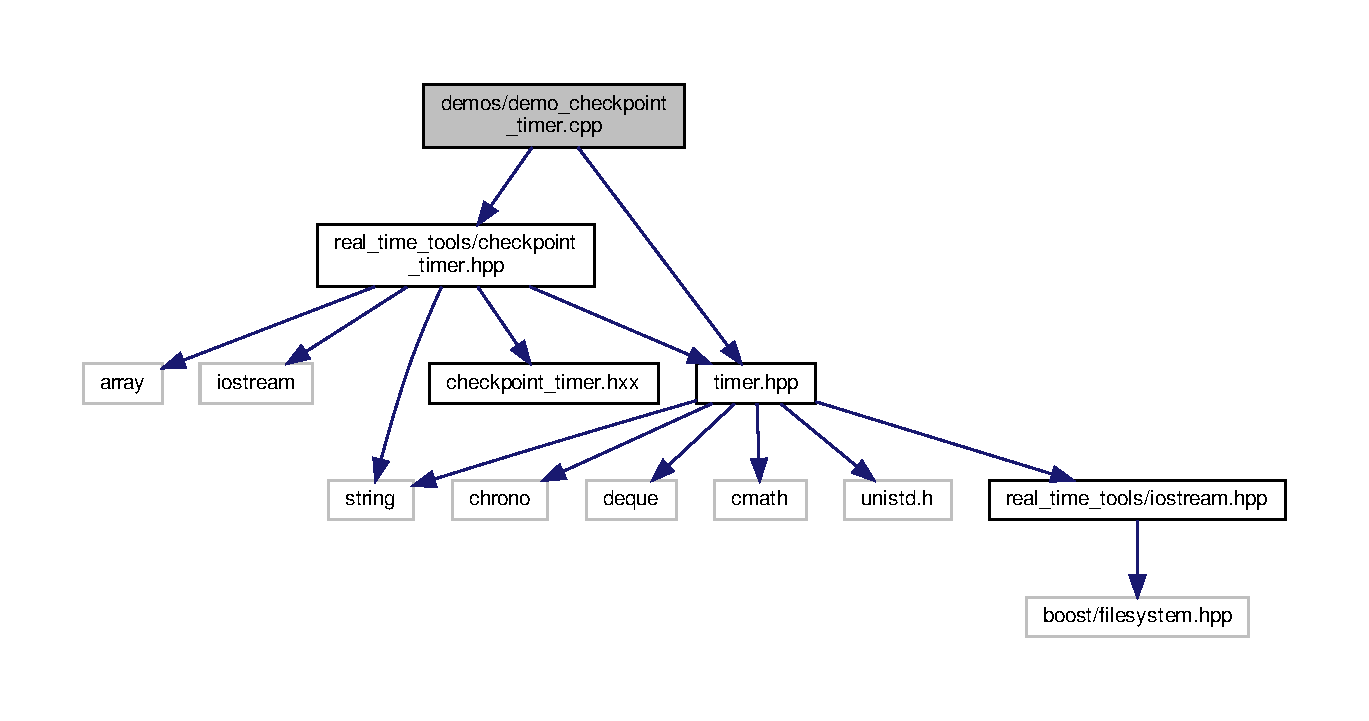
\includegraphics[width=350pt]{demo__checkpoint__timer_8cpp__incl}
\end{center}
\end{figure}
\subsection*{Functions}
\begin{DoxyCompactItemize}
\item 
void \hyperlink{demo__checkpoint__timer_8cpp_a02fd73d861ef2e4aabb38c0c9ff82947}{init} ()\hypertarget{demo__checkpoint__timer_8cpp_a02fd73d861ef2e4aabb38c0c9ff82947}{}\label{demo__checkpoint__timer_8cpp_a02fd73d861ef2e4aabb38c0c9ff82947}

\begin{DoxyCompactList}\small\item\em Dummy function. \end{DoxyCompactList}\item 
void \hyperlink{demo__checkpoint__timer_8cpp_acb546a895e868f1a8fb9cb4b5a210f42}{do\+\_\+some\+\_\+stuff} ()\hypertarget{demo__checkpoint__timer_8cpp_acb546a895e868f1a8fb9cb4b5a210f42}{}\label{demo__checkpoint__timer_8cpp_acb546a895e868f1a8fb9cb4b5a210f42}

\begin{DoxyCompactList}\small\item\em Dummy function. \end{DoxyCompactList}\item 
void \hyperlink{demo__checkpoint__timer_8cpp_a609e6537df0c7eb15c1f5b4e02fbe0ed}{write\+\_\+log} ()\hypertarget{demo__checkpoint__timer_8cpp_a609e6537df0c7eb15c1f5b4e02fbe0ed}{}\label{demo__checkpoint__timer_8cpp_a609e6537df0c7eb15c1f5b4e02fbe0ed}

\begin{DoxyCompactList}\small\item\em Dummy function. \end{DoxyCompactList}\item 
int \hyperlink{demo__checkpoint__timer_8cpp_ae66f6b31b5ad750f1fe042a706a4e3d4}{main} ()
\begin{DoxyCompactList}\small\item\em Simple example on how to use the Checkpoint\+Timer in a loop. \end{DoxyCompactList}\end{DoxyCompactItemize}


\subsection{Detailed Description}
\begin{DoxyRefDesc}{License}
\item[\hyperlink{license__license000001}{License}]B\+SD 3-\/clause \end{DoxyRefDesc}
\begin{DoxyCopyright}{Copyright}
Copyright (c) 2020, New York University and Max Planck Gesellschaft 
\end{DoxyCopyright}


\subsection{Function Documentation}
\index{demo\+\_\+checkpoint\+\_\+timer.\+cpp@{demo\+\_\+checkpoint\+\_\+timer.\+cpp}!main@{main}}
\index{main@{main}!demo\+\_\+checkpoint\+\_\+timer.\+cpp@{demo\+\_\+checkpoint\+\_\+timer.\+cpp}}
\subsubsection[{\texorpdfstring{main()}{main()}}]{\setlength{\rightskip}{0pt plus 5cm}int main (
\begin{DoxyParamCaption}
{}
\end{DoxyParamCaption}
)}\hypertarget{demo__checkpoint__timer_8cpp_ae66f6b31b5ad750f1fe042a706a4e3d4}{}\label{demo__checkpoint__timer_8cpp_ae66f6b31b5ad750f1fe042a706a4e3d4}


Simple example on how to use the Checkpoint\+Timer in a loop. 

\mbox{[}Usage of Checkpoint\+Timer\mbox{]}

\mbox{[}Usage of Checkpoint\+Timer\mbox{]} \begin{Desc}
\item[Examples\+: ]\par
\hyperlink{demo_checkpoint_timer_8cpp-example}{demo\+\_\+checkpoint\+\_\+timer.\+cpp}.\end{Desc}

\hypertarget{demo__realtime__check_8cpp}{}\section{demos/demo\+\_\+realtime\+\_\+check.cpp File Reference}
\label{demo__realtime__check_8cpp}\index{demos/demo\+\_\+realtime\+\_\+check.\+cpp@{demos/demo\+\_\+realtime\+\_\+check.\+cpp}}


Check the real time capbilites of a loop.  


{\ttfamily \#include \char`\"{}real\+\_\+time\+\_\+tools/realtime\+\_\+check.\+hpp\char`\"{}}\newline
{\ttfamily \#include \char`\"{}real\+\_\+time\+\_\+tools/thread.\+hpp\char`\"{}}\newline
{\ttfamily \#include \char`\"{}real\+\_\+time\+\_\+tools/timer.\+hpp\char`\"{}}\newline
Include dependency graph for demo\+\_\+realtime\+\_\+check.\+cpp\+:
\nopagebreak
\begin{figure}[H]
\begin{center}
\leavevmode
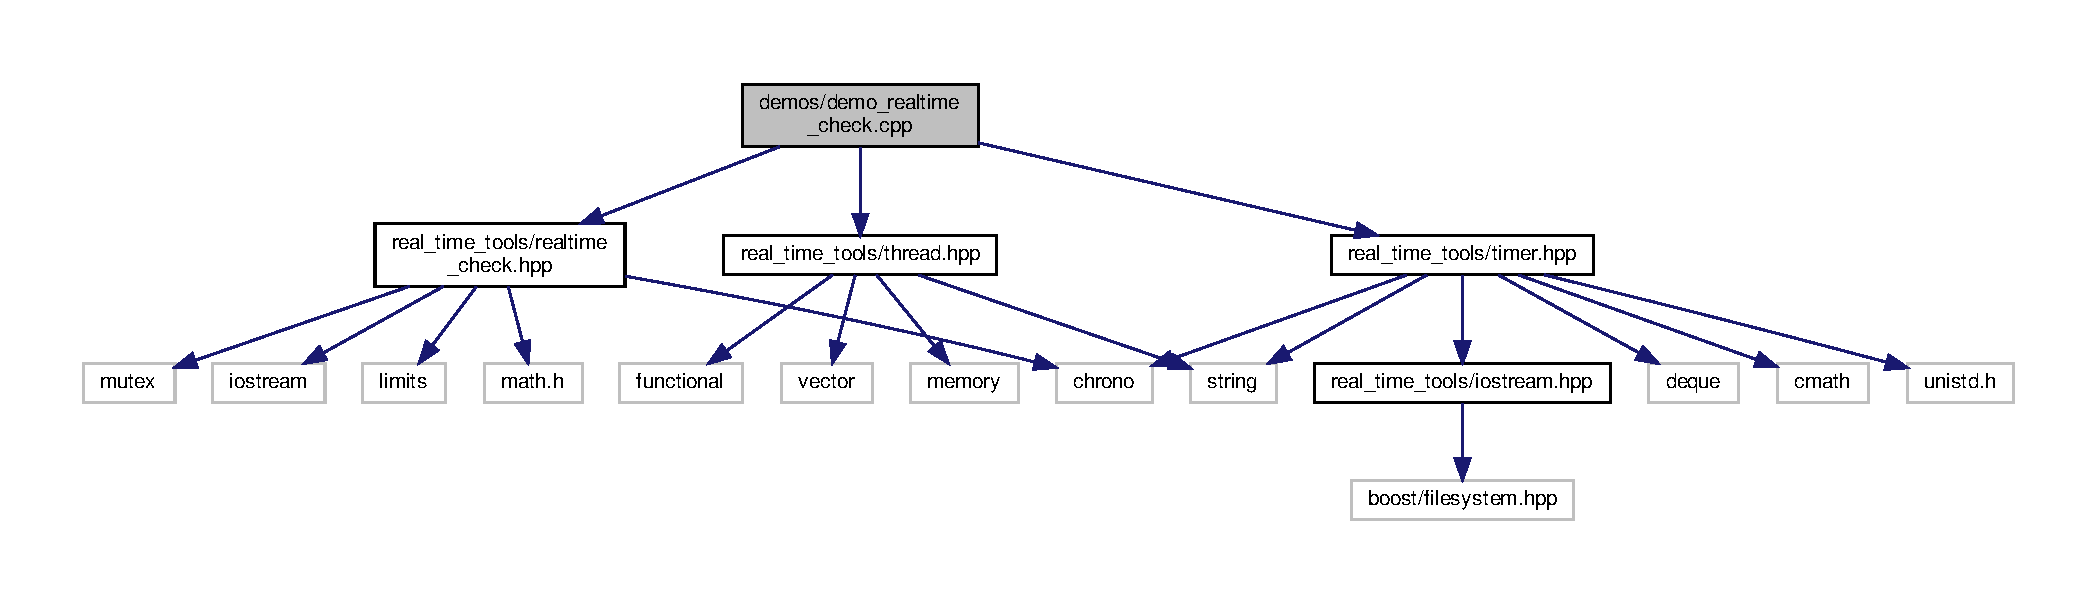
\includegraphics[width=350pt]{demo__realtime__check_8cpp__incl}
\end{center}
\end{figure}
\subsection*{Functions}
\begin{DoxyCompactItemize}
\item 
T\+H\+R\+E\+A\+D\+\_\+\+F\+U\+N\+C\+T\+I\+O\+N\+\_\+\+R\+E\+T\+U\+R\+N\+\_\+\+T\+Y\+PE \hyperlink{demo__realtime__check_8cpp_a16919b2a4211953c87d405d40b432427}{thread\+\_\+function} (void $\ast$)
\item 
int \hyperlink{demo__realtime__check_8cpp_a81ce304348a420752ee080480d2b3095}{main} (int, char $\ast$\mbox{[}$\,$\mbox{]})
\end{DoxyCompactItemize}


\subsection{Detailed Description}
Check the real time capbilites of a loop. 

\begin{DoxyAuthor}{Author}
Maximilien Naveau (\href{mailto:maximilien.naveau@gmail.com}{\tt maximilien.\+naveau@gmail.\+com}) license License B\+S\+D-\/3-\/\+Clause 
\end{DoxyAuthor}
\begin{DoxyCopyright}{Copyright}
Copyright (c) 2019, New York University and Max Planck Gesellschaft. 
\end{DoxyCopyright}
\begin{DoxyDate}{Date}
2019-\/05-\/22 
\end{DoxyDate}


\subsection{Function Documentation}
\mbox{\Hypertarget{demo__realtime__check_8cpp_a81ce304348a420752ee080480d2b3095}\label{demo__realtime__check_8cpp_a81ce304348a420752ee080480d2b3095}} 
\index{demo\+\_\+realtime\+\_\+check.\+cpp@{demo\+\_\+realtime\+\_\+check.\+cpp}!main@{main}}
\index{main@{main}!demo\+\_\+realtime\+\_\+check.\+cpp@{demo\+\_\+realtime\+\_\+check.\+cpp}}
\subsubsection{\texorpdfstring{main()}{main()}}
{\footnotesize\ttfamily int main (\begin{DoxyParamCaption}\item[{int}]{,  }\item[{char $\ast$}]{\mbox{[}$\,$\mbox{]} }\end{DoxyParamCaption})}

Create a real time thread and measure the frequency of the thread. \begin{Desc}
\item[Examples\+: ]\par
\hyperlink{demo_realtime_check_8cpp-example}{demo\+\_\+realtime\+\_\+check.\+cpp}.\end{Desc}
\mbox{\Hypertarget{demo__realtime__check_8cpp_a16919b2a4211953c87d405d40b432427}\label{demo__realtime__check_8cpp_a16919b2a4211953c87d405d40b432427}} 
\index{demo\+\_\+realtime\+\_\+check.\+cpp@{demo\+\_\+realtime\+\_\+check.\+cpp}!thread\+\_\+function@{thread\+\_\+function}}
\index{thread\+\_\+function@{thread\+\_\+function}!demo\+\_\+realtime\+\_\+check.\+cpp@{demo\+\_\+realtime\+\_\+check.\+cpp}}
\subsubsection{\texorpdfstring{thread\+\_\+function()}{thread\_function()}}
{\footnotesize\ttfamily T\+H\+R\+E\+A\+D\+\_\+\+F\+U\+N\+C\+T\+I\+O\+N\+\_\+\+R\+E\+T\+U\+R\+N\+\_\+\+T\+Y\+PE thread\+\_\+function (\begin{DoxyParamCaption}\item[{void $\ast$}]{ }\end{DoxyParamCaption})}

Real time thread that measure the spinning frequency and do some basic operation \begin{Desc}
\item[Examples\+: ]\par
\hyperlink{demo_realtime_check_8cpp-example}{demo\+\_\+realtime\+\_\+check.\+cpp}.\end{Desc}

\hypertarget{demo__realtime__strict__check_8cpp}{}\section{demos/demo\+\_\+realtime\+\_\+strict\+\_\+check.cpp File Reference}
\label{demo__realtime__strict__check_8cpp}\index{demos/demo\+\_\+realtime\+\_\+strict\+\_\+check.\+cpp@{demos/demo\+\_\+realtime\+\_\+strict\+\_\+check.\+cpp}}


Check the real time capbilites of a loop.  


{\ttfamily \#include \char`\"{}real\+\_\+time\+\_\+tools/realtime\+\_\+check.\+hpp\char`\"{}}\\*
{\ttfamily \#include \char`\"{}real\+\_\+time\+\_\+tools/thread.\+hpp\char`\"{}}\\*
Include dependency graph for demo\+\_\+realtime\+\_\+strict\+\_\+check.\+cpp\+:
\nopagebreak
\begin{figure}[H]
\begin{center}
\leavevmode
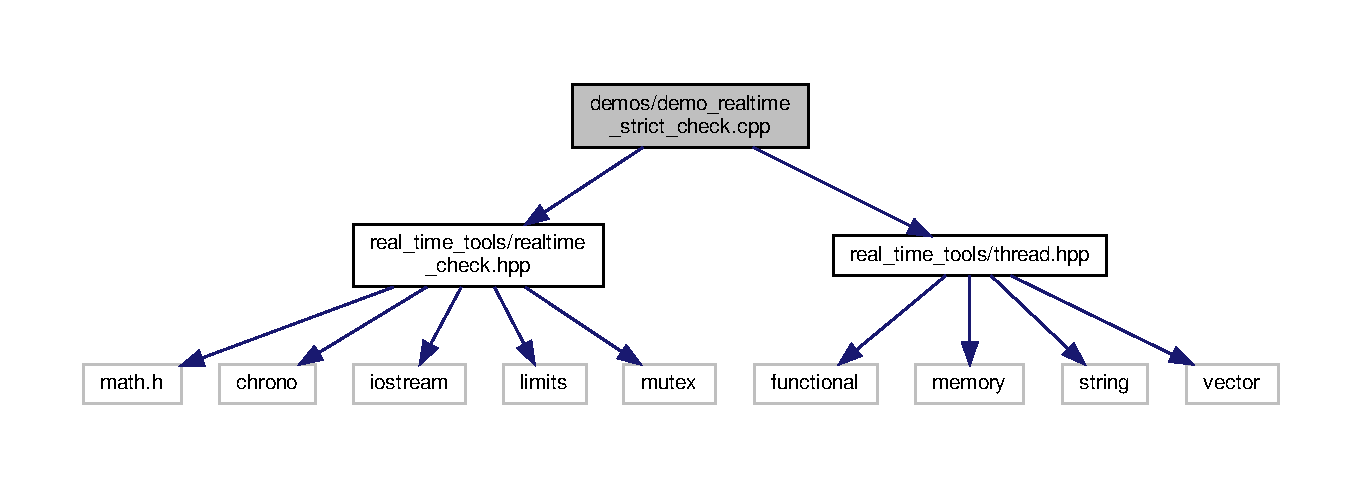
\includegraphics[width=350pt]{demo__realtime__strict__check_8cpp__incl}
\end{center}
\end{figure}
\subsection*{Typedefs}
\begin{DoxyCompactItemize}
\item 
typedef std\+::chrono\+::high\+\_\+resolution\+\_\+clock \hyperlink{demo__realtime__strict__check_8cpp_a3b195616f5dbd3a9cae7f618efe85b9b}{my\+\_\+clock}\hypertarget{demo__realtime__strict__check_8cpp_a3b195616f5dbd3a9cae7f618efe85b9b}{}\label{demo__realtime__strict__check_8cpp_a3b195616f5dbd3a9cae7f618efe85b9b}

\begin{DoxyCompactList}\small\item\em define an alias for the clock \end{DoxyCompactList}\end{DoxyCompactItemize}
\subsection*{Functions}
\begin{DoxyCompactItemize}
\item 
T\+H\+R\+E\+A\+D\+\_\+\+F\+U\+N\+C\+T\+I\+O\+N\+\_\+\+R\+E\+T\+U\+R\+N\+\_\+\+T\+Y\+PE \hyperlink{demo__realtime__strict__check_8cpp_a16919b2a4211953c87d405d40b432427}{thread\+\_\+function} (void $\ast$)
\begin{DoxyCompactList}\small\item\em this function is executed in a real\+\_\+time\+\_\+thread. \end{DoxyCompactList}\item 
int \hyperlink{demo__realtime__strict__check_8cpp_a81ce304348a420752ee080480d2b3095}{main} (int, char $\ast$\mbox{[}$\,$\mbox{]})
\begin{DoxyCompactList}\small\item\em This demos show the used of the strict check of the real time loop. \end{DoxyCompactList}\end{DoxyCompactItemize}


\subsection{Detailed Description}
Check the real time capbilites of a loop. 

\begin{DoxyAuthor}{Author}
Maximilien Naveau (\href{mailto:maximilien.naveau@gmail.com}{\tt maximilien.\+naveau@gmail.\+com}) license License B\+S\+D-\/3-\/\+Clause 
\end{DoxyAuthor}
\begin{DoxyCopyright}{Copyright}
Copyright (c) 2019, New York University and Max Planck Gesellschaft. 
\end{DoxyCopyright}
\begin{DoxyDate}{Date}
2019-\/05-\/22 
\end{DoxyDate}


\subsection{Function Documentation}
\index{demo\+\_\+realtime\+\_\+strict\+\_\+check.\+cpp@{demo\+\_\+realtime\+\_\+strict\+\_\+check.\+cpp}!main@{main}}
\index{main@{main}!demo\+\_\+realtime\+\_\+strict\+\_\+check.\+cpp@{demo\+\_\+realtime\+\_\+strict\+\_\+check.\+cpp}}
\subsubsection[{\texorpdfstring{main(int, char $\ast$[])}{main(int, char *[])}}]{\setlength{\rightskip}{0pt plus 5cm}int main (
\begin{DoxyParamCaption}
\item[{int}]{, }
\item[{char $\ast$}]{\mbox{[}$\,$\mbox{]}}
\end{DoxyParamCaption}
)}\hypertarget{demo__realtime__strict__check_8cpp_a81ce304348a420752ee080480d2b3095}{}\label{demo__realtime__strict__check_8cpp_a81ce304348a420752ee080480d2b3095}


This demos show the used of the strict check of the real time loop. 

\begin{Desc}
\item[Examples\+: ]\par
\hyperlink{demo_realtime_strict_check_8cpp-example}{demo\+\_\+realtime\+\_\+strict\+\_\+check.\+cpp}.\end{Desc}
\index{demo\+\_\+realtime\+\_\+strict\+\_\+check.\+cpp@{demo\+\_\+realtime\+\_\+strict\+\_\+check.\+cpp}!thread\+\_\+function@{thread\+\_\+function}}
\index{thread\+\_\+function@{thread\+\_\+function}!demo\+\_\+realtime\+\_\+strict\+\_\+check.\+cpp@{demo\+\_\+realtime\+\_\+strict\+\_\+check.\+cpp}}
\subsubsection[{\texorpdfstring{thread\+\_\+function(void $\ast$)}{thread_function(void *)}}]{\setlength{\rightskip}{0pt plus 5cm}T\+H\+R\+E\+A\+D\+\_\+\+F\+U\+N\+C\+T\+I\+O\+N\+\_\+\+R\+E\+T\+U\+R\+N\+\_\+\+T\+Y\+PE thread\+\_\+function (
\begin{DoxyParamCaption}
\item[{void $\ast$}]{}
\end{DoxyParamCaption}
)}\hypertarget{demo__realtime__strict__check_8cpp_a16919b2a4211953c87d405d40b432427}{}\label{demo__realtime__strict__check_8cpp_a16919b2a4211953c87d405d40b432427}


this function is executed in a real\+\_\+time\+\_\+thread. 

\begin{Desc}
\item[Examples\+: ]\par
\hyperlink{demo_realtime_strict_check_8cpp-example}{demo\+\_\+realtime\+\_\+strict\+\_\+check.\+cpp}.\end{Desc}

\hypertarget{demo__spinner_8cpp}{}\section{demos/demo\+\_\+spinner.cpp File Reference}
\label{demo__spinner_8cpp}\index{demos/demo\+\_\+spinner.\+cpp@{demos/demo\+\_\+spinner.\+cpp}}


Demo of the spinner class usage.  


{\ttfamily \#include \char`\"{}real\+\_\+time\+\_\+tools/realtime\+\_\+check.\+hpp\char`\"{}}\newline
{\ttfamily \#include \char`\"{}real\+\_\+time\+\_\+tools/spinner.\+hpp\char`\"{}}\newline
{\ttfamily \#include \char`\"{}real\+\_\+time\+\_\+tools/thread.\+hpp\char`\"{}}\newline
Include dependency graph for demo\+\_\+spinner.\+cpp\+:
\nopagebreak
\begin{figure}[H]
\begin{center}
\leavevmode
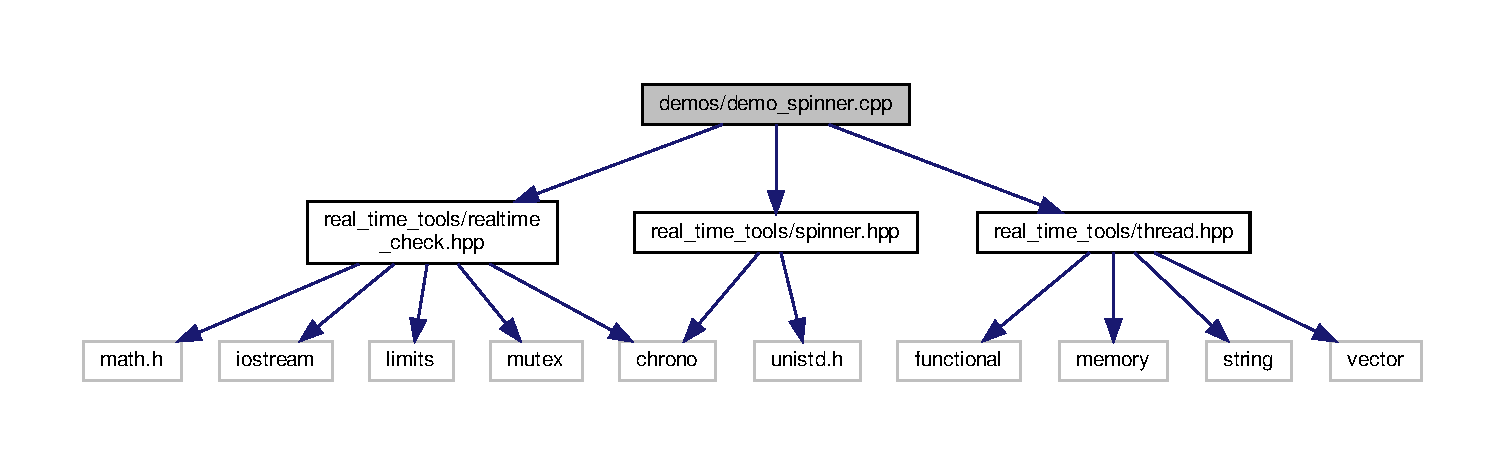
\includegraphics[width=350pt]{demo__spinner_8cpp__incl}
\end{center}
\end{figure}
\subsection*{Functions}
\begin{DoxyCompactItemize}
\item 
\mbox{\Hypertarget{demo__spinner_8cpp_a16919b2a4211953c87d405d40b432427}\label{demo__spinner_8cpp_a16919b2a4211953c87d405d40b432427}} 
T\+H\+R\+E\+A\+D\+\_\+\+F\+U\+N\+C\+T\+I\+O\+N\+\_\+\+R\+E\+T\+U\+R\+N\+\_\+\+T\+Y\+PE \hyperlink{demo__spinner_8cpp_a16919b2a4211953c87d405d40b432427}{thread\+\_\+function} (void $\ast$)
\begin{DoxyCompactList}\small\item\em implement a real time thread checking the timing of the loop \end{DoxyCompactList}\item 
int \hyperlink{demo__spinner_8cpp_a81ce304348a420752ee080480d2b3095}{main} (int, char $\ast$\mbox{[}$\,$\mbox{]})
\begin{DoxyCompactList}\small\item\em This a demo on how to use the Real\+Time\+Check class. \end{DoxyCompactList}\end{DoxyCompactItemize}


\subsection{Detailed Description}
Demo of the spinner class usage. 

\begin{DoxyAuthor}{Author}
Maximilien Naveau (\href{mailto:maximilien.naveau@gmail.com}{\tt maximilien.\+naveau@gmail.\+com}) license License B\+S\+D-\/3-\/\+Clause 
\end{DoxyAuthor}
\begin{DoxyCopyright}{Copyright}
Copyright (c) 2019, New York University and Max Planck Gesellschaft. 
\end{DoxyCopyright}
\begin{DoxyDate}{Date}
2019-\/05-\/22 
\end{DoxyDate}


\subsection{Function Documentation}
\mbox{\Hypertarget{demo__spinner_8cpp_a81ce304348a420752ee080480d2b3095}\label{demo__spinner_8cpp_a81ce304348a420752ee080480d2b3095}} 
\index{demo\+\_\+spinner.\+cpp@{demo\+\_\+spinner.\+cpp}!main@{main}}
\index{main@{main}!demo\+\_\+spinner.\+cpp@{demo\+\_\+spinner.\+cpp}}
\subsubsection{\texorpdfstring{main()}{main()}}
{\footnotesize\ttfamily int main (\begin{DoxyParamCaption}\item[{int}]{,  }\item[{char $\ast$}]{\mbox{[}$\,$\mbox{]} }\end{DoxyParamCaption})}



This a demo on how to use the Real\+Time\+Check class. 

\begin{Desc}
\item[Examples\+: ]\par
\hyperlink{demo_spinner_8cpp-example}{demo\+\_\+spinner.\+cpp}.\end{Desc}

\hypertarget{demo__thread_8cpp}{}\section{demos/demo\+\_\+thread.cpp File Reference}
\label{demo__thread_8cpp}\index{demos/demo\+\_\+thread.\+cpp@{demos/demo\+\_\+thread.\+cpp}}


Mininal thread example.  


{\ttfamily \#include \char`\"{}real\+\_\+time\+\_\+tools/thread.\+hpp\char`\"{}}\\*
{\ttfamily \#include \char`\"{}real\+\_\+time\+\_\+tools/timer.\+hpp\char`\"{}}\\*
Include dependency graph for demo\+\_\+thread.\+cpp\+:
\nopagebreak
\begin{figure}[H]
\begin{center}
\leavevmode
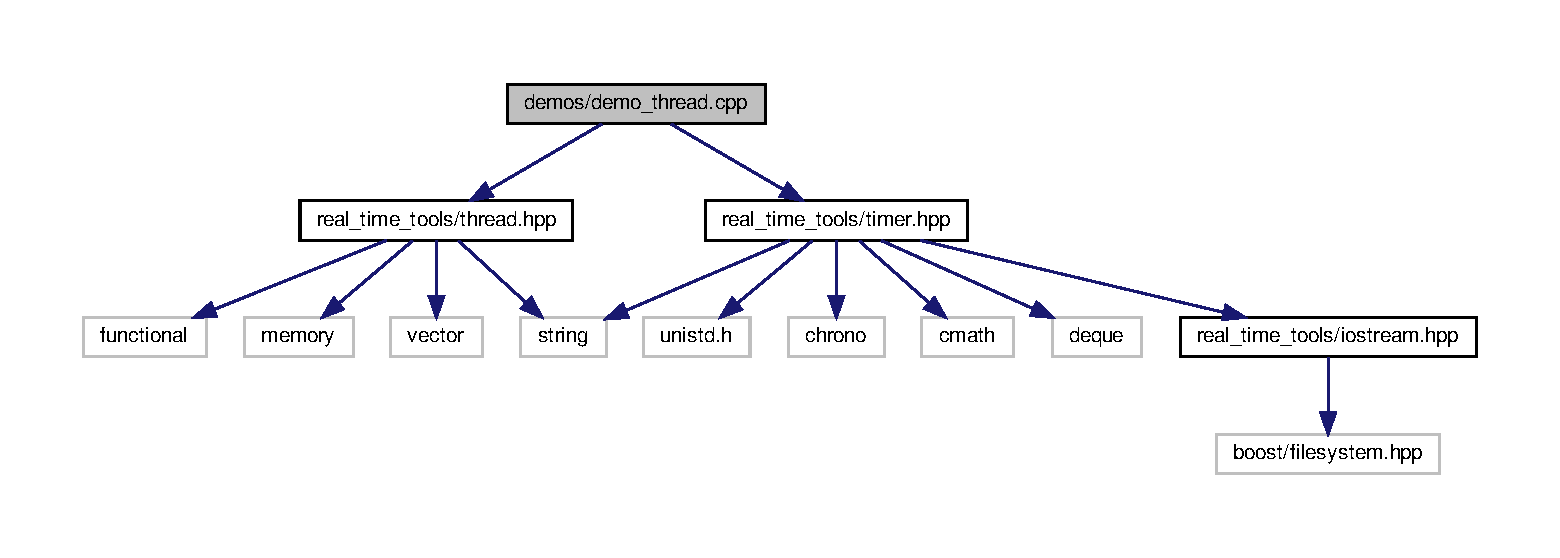
\includegraphics[width=350pt]{demo__thread_8cpp__incl}
\end{center}
\end{figure}
\subsection*{Functions}
\begin{DoxyCompactItemize}
\item 
T\+H\+R\+E\+A\+D\+\_\+\+F\+U\+N\+C\+T\+I\+O\+N\+\_\+\+R\+E\+T\+U\+R\+N\+\_\+\+T\+Y\+PE {\bfseries thread\+\_\+function} (void $\ast$)\hypertarget{demo__thread_8cpp_a16919b2a4211953c87d405d40b432427}{}\label{demo__thread_8cpp_a16919b2a4211953c87d405d40b432427}

\item 
int {\bfseries main} ()\hypertarget{demo__thread_8cpp_ae66f6b31b5ad750f1fe042a706a4e3d4}{}\label{demo__thread_8cpp_ae66f6b31b5ad750f1fe042a706a4e3d4}

\end{DoxyCompactItemize}


\subsection{Detailed Description}
Mininal thread example. 

\begin{DoxyAuthor}{Author}
Vincent Berenz license License B\+S\+D-\/3-\/\+Clause 
\end{DoxyAuthor}
\begin{DoxyCopyright}{Copyright}
Copyright (c) 2019, New York University and Max Planck Gesellschaft. 
\end{DoxyCopyright}
\begin{DoxyDate}{Date}
2020-\/01-\/02 
\end{DoxyDate}

\hypertarget{demo__timing_8cpp}{}\section{demos/demo\+\_\+timing.cpp File Reference}
\label{demo__timing_8cpp}\index{demos/demo\+\_\+timing.\+cpp@{demos/demo\+\_\+timing.\+cpp}}


Demo of the Timer class usage.  


{\ttfamily \#include \char`\"{}real\+\_\+time\+\_\+tools/spinner.\+hpp\char`\"{}}\\*
{\ttfamily \#include \char`\"{}real\+\_\+time\+\_\+tools/thread.\+hpp\char`\"{}}\\*
{\ttfamily \#include \char`\"{}real\+\_\+time\+\_\+tools/realtime\+\_\+check.\+hpp\char`\"{}}\\*
{\ttfamily \#include \char`\"{}real\+\_\+time\+\_\+tools/timer.\+hpp\char`\"{}}\\*
Include dependency graph for demo\+\_\+timing.\+cpp\+:
\nopagebreak
\begin{figure}[H]
\begin{center}
\leavevmode
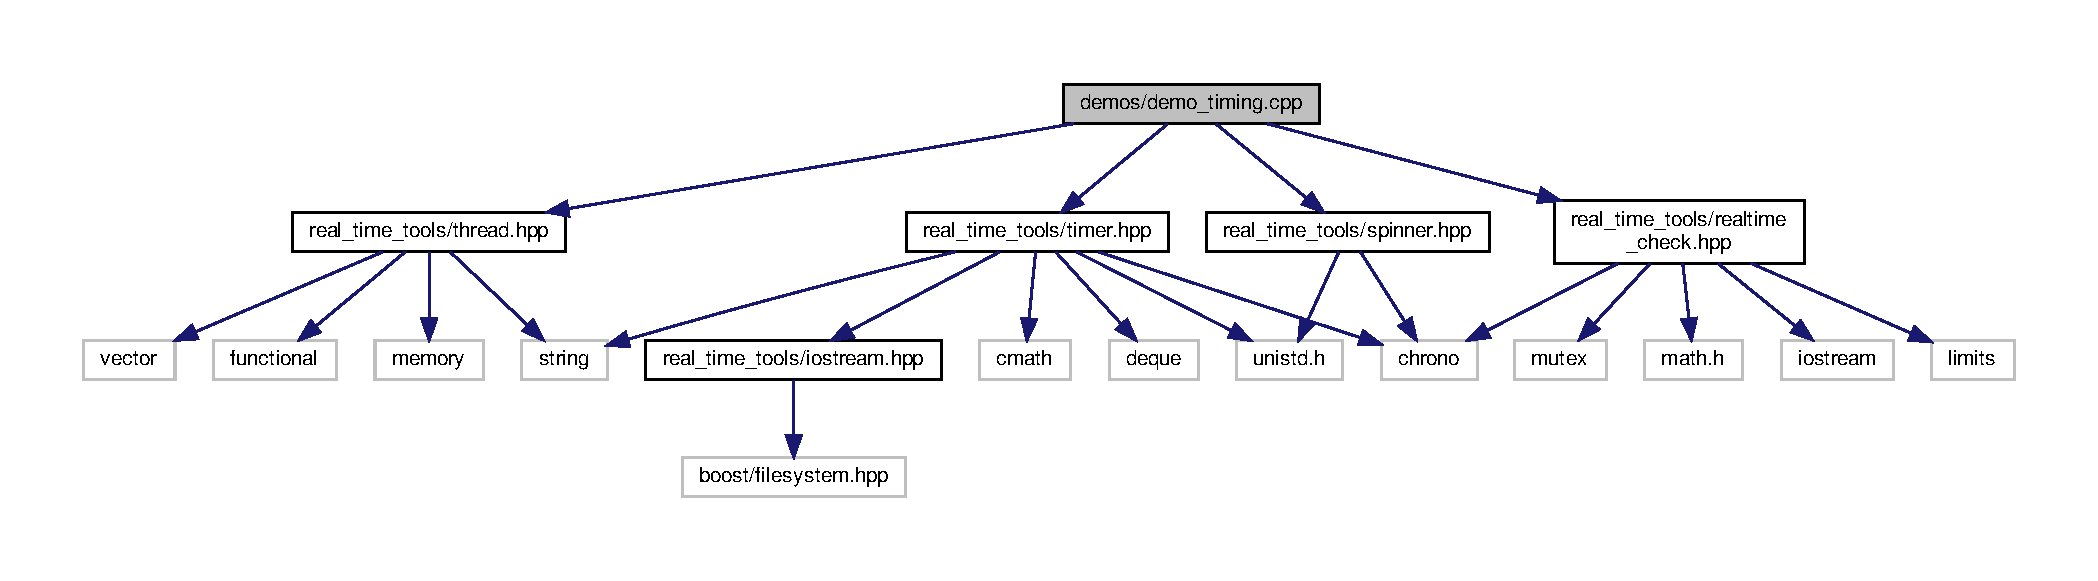
\includegraphics[width=350pt]{demo__timing_8cpp__incl}
\end{center}
\end{figure}
\subsection*{Functions}
\begin{DoxyCompactItemize}
\item 
T\+H\+R\+E\+A\+D\+\_\+\+F\+U\+N\+C\+T\+I\+O\+N\+\_\+\+R\+E\+T\+U\+R\+N\+\_\+\+T\+Y\+PE \hyperlink{demo__timing_8cpp_a16919b2a4211953c87d405d40b432427}{thread\+\_\+function} (void $\ast$)
\begin{DoxyCompactList}\small\item\em Real time thread presenting the use of the Timer class. \end{DoxyCompactList}\item 
int \hyperlink{demo__timing_8cpp_a81ce304348a420752ee080480d2b3095}{main} (int, char $\ast$\mbox{[}$\,$\mbox{]})
\begin{DoxyCompactList}\small\item\em Launch a real time thread presenting the use of the Timer class. \end{DoxyCompactList}\end{DoxyCompactItemize}


\subsection{Detailed Description}
Demo of the Timer class usage. 

\begin{DoxyAuthor}{Author}
Maximilien Naveau (\href{mailto:maximilien.naveau@gmail.com}{\tt maximilien.\+naveau@gmail.\+com}) license License B\+S\+D-\/3-\/\+Clause 
\end{DoxyAuthor}
\begin{DoxyCopyright}{Copyright}
Copyright (c) 2019, New York University and Max Planck Gesellschaft. 
\end{DoxyCopyright}
\begin{DoxyDate}{Date}
2019-\/05-\/22 
\end{DoxyDate}


\subsection{Function Documentation}
\index{demo\+\_\+timing.\+cpp@{demo\+\_\+timing.\+cpp}!main@{main}}
\index{main@{main}!demo\+\_\+timing.\+cpp@{demo\+\_\+timing.\+cpp}}
\subsubsection[{\texorpdfstring{main(int, char $\ast$[])}{main(int, char *[])}}]{\setlength{\rightskip}{0pt plus 5cm}int main (
\begin{DoxyParamCaption}
\item[{int}]{, }
\item[{char $\ast$}]{\mbox{[}$\,$\mbox{]}}
\end{DoxyParamCaption}
)}\hypertarget{demo__timing_8cpp_a81ce304348a420752ee080480d2b3095}{}\label{demo__timing_8cpp_a81ce304348a420752ee080480d2b3095}


Launch a real time thread presenting the use of the Timer class. 

\begin{Desc}
\item[Examples\+: ]\par
\hyperlink{demo_timing_8cpp-example}{demo\+\_\+timing.\+cpp}.\end{Desc}
\index{demo\+\_\+timing.\+cpp@{demo\+\_\+timing.\+cpp}!thread\+\_\+function@{thread\+\_\+function}}
\index{thread\+\_\+function@{thread\+\_\+function}!demo\+\_\+timing.\+cpp@{demo\+\_\+timing.\+cpp}}
\subsubsection[{\texorpdfstring{thread\+\_\+function(void $\ast$)}{thread_function(void *)}}]{\setlength{\rightskip}{0pt plus 5cm}T\+H\+R\+E\+A\+D\+\_\+\+F\+U\+N\+C\+T\+I\+O\+N\+\_\+\+R\+E\+T\+U\+R\+N\+\_\+\+T\+Y\+PE thread\+\_\+function (
\begin{DoxyParamCaption}
\item[{void $\ast$}]{}
\end{DoxyParamCaption}
)}\hypertarget{demo__timing_8cpp_a16919b2a4211953c87d405d40b432427}{}\label{demo__timing_8cpp_a16919b2a4211953c87d405d40b432427}


Real time thread presenting the use of the Timer class. 

\begin{Desc}
\item[Examples\+: ]\par
\hyperlink{demo_timing_8cpp-example}{demo\+\_\+timing.\+cpp}.\end{Desc}

\hypertarget{demo__usb__stream__imu__3DM__GX3__25_8cpp}{}\section{demos/demo\+\_\+usb\+\_\+stream\+\_\+imu\+\_\+3\+D\+M\+\_\+\+G\+X3\+\_\+25.cpp File Reference}
\label{demo__usb__stream__imu__3DM__GX3__25_8cpp}\index{demos/demo\+\_\+usb\+\_\+stream\+\_\+imu\+\_\+3\+D\+M\+\_\+\+G\+X3\+\_\+25.\+cpp@{demos/demo\+\_\+usb\+\_\+stream\+\_\+imu\+\_\+3\+D\+M\+\_\+\+G\+X3\+\_\+25.\+cpp}}


Testing imu connection directly via the drivers. See test\+\_\+interface in the same package for an example of the A\+PI.  


{\ttfamily \#include \char`\"{}real\+\_\+time\+\_\+tools/timer.\+hpp\char`\"{}}\newline
{\ttfamily \#include \char`\"{}real\+\_\+time\+\_\+tools/usb\+\_\+stream.\+hpp\char`\"{}}\newline
Include dependency graph for demo\+\_\+usb\+\_\+stream\+\_\+imu\+\_\+3\+D\+M\+\_\+\+G\+X3\+\_\+25.\+cpp\+:
\nopagebreak
\begin{figure}[H]
\begin{center}
\leavevmode
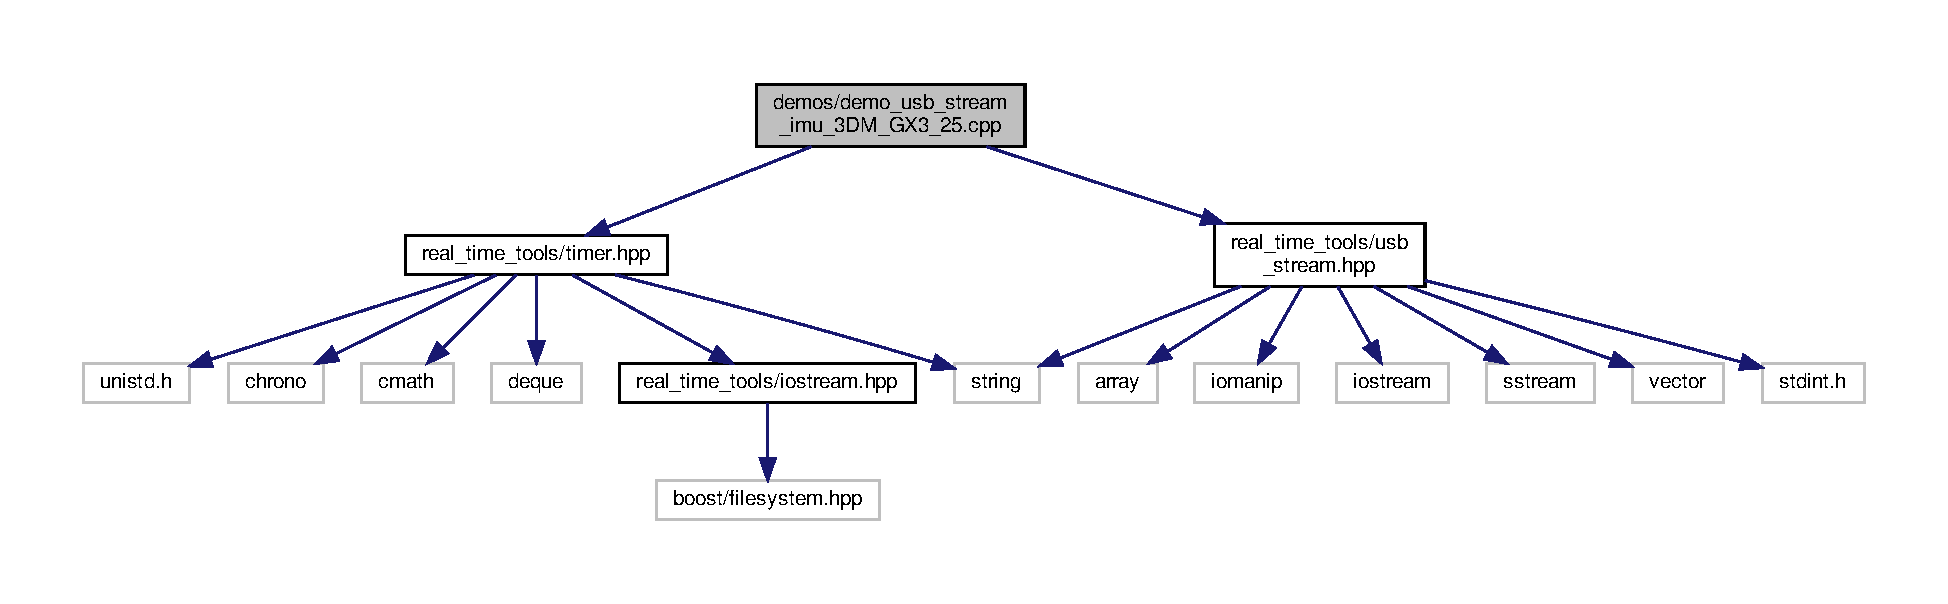
\includegraphics[width=350pt]{demo__usb__stream__imu__3DM__GX3__25_8cpp__incl}
\end{center}
\end{figure}
\subsection*{Functions}
\begin{DoxyCompactItemize}
\item 
void \hyperlink{demo__usb__stream__imu__3DM__GX3__25_8cpp_af411ef352aef0f8d040d8d60c49eac7a}{continuous\+\_\+mode\+\_\+on} (\hyperlink{classreal__time__tools_1_1UsbStream}{real\+\_\+time\+\_\+tools\+::\+Usb\+Stream} \&usb\+\_\+stream, bool stream\+\_\+mode)
\begin{DoxyCompactList}\small\item\em Send the message that set the imu into stream mode or not. \end{DoxyCompactList}\item 
bool \hyperlink{demo__usb__stream__imu__3DM__GX3__25_8cpp_a8a096d7f567dad6d28f0fd870ba6bb43}{is\+\_\+continuous\+\_\+mode\+\_\+on} (\hyperlink{classreal__time__tools_1_1UsbStream}{real\+\_\+time\+\_\+tools\+::\+Usb\+Stream} \&usb\+\_\+stream, bool stream\+\_\+mode)
\begin{DoxyCompactList}\small\item\em Check the mode of the imu. \end{DoxyCompactList}\item 
void \hyperlink{demo__usb__stream__imu__3DM__GX3__25_8cpp_a1d00f7ae49ec05ecaf8ecd4d76129573}{continuous\+\_\+mode\+\_\+off} (\hyperlink{classreal__time__tools_1_1UsbStream}{real\+\_\+time\+\_\+tools\+::\+Usb\+Stream} \&usb\+\_\+stream, bool stream\+\_\+mode)
\begin{DoxyCompactList}\small\item\em Set the imu into idle mode. \end{DoxyCompactList}\item 
void \hyperlink{demo__usb__stream__imu__3DM__GX3__25_8cpp_af04ed9328c659fc57f91d74cdeedda72}{reset} (\hyperlink{classreal__time__tools_1_1UsbStream}{real\+\_\+time\+\_\+tools\+::\+Usb\+Stream} \&usb\+\_\+stream, bool stream\+\_\+mode)
\begin{DoxyCompactList}\small\item\em Reset the imu. \end{DoxyCompactList}\item 
int \hyperlink{demo__usb__stream__imu__3DM__GX3__25_8cpp_a3c04138a5bfe5d72780bb7e82a18e627}{main} (int argc, char $\ast$$\ast$argv)
\begin{DoxyCompactList}\small\item\em Example on how to use the usb interface using an imu. \end{DoxyCompactList}\end{DoxyCompactItemize}


\subsection{Detailed Description}
Testing imu connection directly via the drivers. See test\+\_\+interface in the same package for an example of the A\+PI. 

\begin{DoxyAuthor}{Author}
Vincent Berenz (\href{mailto:vincent.brenz@tuebingen.mpg.de}{\tt vincent.\+brenz@tuebingen.\+mpg.\+de}) 
\end{DoxyAuthor}
\begin{DoxyVersion}{Version}
0.\+1 
\end{DoxyVersion}
\begin{DoxyDate}{Date}
2019-\/05-\/09
\end{DoxyDate}
\begin{DoxyCopyright}{Copyright}
Copyright (c) 2019 
\end{DoxyCopyright}


\subsection{Function Documentation}
\mbox{\Hypertarget{demo__usb__stream__imu__3DM__GX3__25_8cpp_a1d00f7ae49ec05ecaf8ecd4d76129573}\label{demo__usb__stream__imu__3DM__GX3__25_8cpp_a1d00f7ae49ec05ecaf8ecd4d76129573}} 
\index{demo\+\_\+usb\+\_\+stream\+\_\+imu\+\_\+3\+D\+M\+\_\+\+G\+X3\+\_\+25.\+cpp@{demo\+\_\+usb\+\_\+stream\+\_\+imu\+\_\+3\+D\+M\+\_\+\+G\+X3\+\_\+25.\+cpp}!continuous\+\_\+mode\+\_\+off@{continuous\+\_\+mode\+\_\+off}}
\index{continuous\+\_\+mode\+\_\+off@{continuous\+\_\+mode\+\_\+off}!demo\+\_\+usb\+\_\+stream\+\_\+imu\+\_\+3\+D\+M\+\_\+\+G\+X3\+\_\+25.\+cpp@{demo\+\_\+usb\+\_\+stream\+\_\+imu\+\_\+3\+D\+M\+\_\+\+G\+X3\+\_\+25.\+cpp}}
\subsubsection{\texorpdfstring{continuous\+\_\+mode\+\_\+off()}{continuous\_mode\_off()}}
{\footnotesize\ttfamily void continuous\+\_\+mode\+\_\+off (\begin{DoxyParamCaption}\item[{\hyperlink{classreal__time__tools_1_1UsbStream}{real\+\_\+time\+\_\+tools\+::\+Usb\+Stream} \&}]{usb\+\_\+stream,  }\item[{bool}]{stream\+\_\+mode }\end{DoxyParamCaption})}



Set the imu into idle mode. 


\begin{DoxyParams}{Parameters}
{\em usb\+\_\+stream} & \\
\hline
{\em stream\+\_\+mode} & \\
\hline
\end{DoxyParams}
Here we set the I\+MU into a constant broadcasting mode. The broadcasted data are composed with the accelerometer and the gyroscope. \href{https://atlas.is.localnet/confluence/display/AMDW/Microstrain+3DM+IMUs?preview=/8979810/17761244/3DM-GX3-Data-Communications-Protocol.pdf}{\tt https\+://atlas.\+is.\+localnet/confluence/display/\+A\+M\+D\+W/\+Microstrain+3\+D\+M+\+I\+M\+Us?preview=/8979810/17761244/3\+D\+M-\/\+G\+X3-\/\+Data-\/\+Communications-\/\+Protocol.\+pdf}\begin{Desc}
\item[Examples\+: ]\par
\hyperlink{demo_usb_stream_imu_3DM_GX3_25_8cpp-example}{demo\+\_\+usb\+\_\+stream\+\_\+imu\+\_\+3\+D\+M\+\_\+\+G\+X3\+\_\+25.\+cpp}.\end{Desc}
\mbox{\Hypertarget{demo__usb__stream__imu__3DM__GX3__25_8cpp_af411ef352aef0f8d040d8d60c49eac7a}\label{demo__usb__stream__imu__3DM__GX3__25_8cpp_af411ef352aef0f8d040d8d60c49eac7a}} 
\index{demo\+\_\+usb\+\_\+stream\+\_\+imu\+\_\+3\+D\+M\+\_\+\+G\+X3\+\_\+25.\+cpp@{demo\+\_\+usb\+\_\+stream\+\_\+imu\+\_\+3\+D\+M\+\_\+\+G\+X3\+\_\+25.\+cpp}!continuous\+\_\+mode\+\_\+on@{continuous\+\_\+mode\+\_\+on}}
\index{continuous\+\_\+mode\+\_\+on@{continuous\+\_\+mode\+\_\+on}!demo\+\_\+usb\+\_\+stream\+\_\+imu\+\_\+3\+D\+M\+\_\+\+G\+X3\+\_\+25.\+cpp@{demo\+\_\+usb\+\_\+stream\+\_\+imu\+\_\+3\+D\+M\+\_\+\+G\+X3\+\_\+25.\+cpp}}
\subsubsection{\texorpdfstring{continuous\+\_\+mode\+\_\+on()}{continuous\_mode\_on()}}
{\footnotesize\ttfamily void continuous\+\_\+mode\+\_\+on (\begin{DoxyParamCaption}\item[{\hyperlink{classreal__time__tools_1_1UsbStream}{real\+\_\+time\+\_\+tools\+::\+Usb\+Stream} \&}]{usb\+\_\+stream,  }\item[{bool}]{stream\+\_\+mode }\end{DoxyParamCaption})}



Send the message that set the imu into stream mode or not. 


\begin{DoxyParams}{Parameters}
{\em usb\+\_\+stream} & is the usb interface. \\
\hline
{\em stream\+\_\+mode} & start or stop the stream mode. \\
\hline
\end{DoxyParams}
Here we set the I\+MU into a constant broadcasting mode. The broadcasted data are composed with the accelerometer and the gyroscope. \href{https://atlas.is.localnet/confluence/display/AMDW/Microstrain+3DM+IMUs?preview=/8979810/17761244/3DM-GX3-Data-Communications-Protocol.pdf}{\tt https\+://atlas.\+is.\+localnet/confluence/display/\+A\+M\+D\+W/\+Microstrain+3\+D\+M+\+I\+M\+Us?preview=/8979810/17761244/3\+D\+M-\/\+G\+X3-\/\+Data-\/\+Communications-\/\+Protocol.\+pdf}\begin{Desc}
\item[Examples\+: ]\par
\hyperlink{demo_usb_stream_imu_3DM_GX3_25_8cpp-example}{demo\+\_\+usb\+\_\+stream\+\_\+imu\+\_\+3\+D\+M\+\_\+\+G\+X3\+\_\+25.\+cpp}.\end{Desc}
\mbox{\Hypertarget{demo__usb__stream__imu__3DM__GX3__25_8cpp_a8a096d7f567dad6d28f0fd870ba6bb43}\label{demo__usb__stream__imu__3DM__GX3__25_8cpp_a8a096d7f567dad6d28f0fd870ba6bb43}} 
\index{demo\+\_\+usb\+\_\+stream\+\_\+imu\+\_\+3\+D\+M\+\_\+\+G\+X3\+\_\+25.\+cpp@{demo\+\_\+usb\+\_\+stream\+\_\+imu\+\_\+3\+D\+M\+\_\+\+G\+X3\+\_\+25.\+cpp}!is\+\_\+continuous\+\_\+mode\+\_\+on@{is\+\_\+continuous\+\_\+mode\+\_\+on}}
\index{is\+\_\+continuous\+\_\+mode\+\_\+on@{is\+\_\+continuous\+\_\+mode\+\_\+on}!demo\+\_\+usb\+\_\+stream\+\_\+imu\+\_\+3\+D\+M\+\_\+\+G\+X3\+\_\+25.\+cpp@{demo\+\_\+usb\+\_\+stream\+\_\+imu\+\_\+3\+D\+M\+\_\+\+G\+X3\+\_\+25.\+cpp}}
\subsubsection{\texorpdfstring{is\+\_\+continuous\+\_\+mode\+\_\+on()}{is\_continuous\_mode\_on()}}
{\footnotesize\ttfamily bool is\+\_\+continuous\+\_\+mode\+\_\+on (\begin{DoxyParamCaption}\item[{\hyperlink{classreal__time__tools_1_1UsbStream}{real\+\_\+time\+\_\+tools\+::\+Usb\+Stream} \&}]{usb\+\_\+stream,  }\item[{bool}]{stream\+\_\+mode }\end{DoxyParamCaption})}



Check the mode of the imu. 


\begin{DoxyParams}{Parameters}
{\em usb\+\_\+stream} & usb communication interface. \\
\hline
{\em stream\+\_\+mode} & read the socket in stream mode or not. \\
\hline
\end{DoxyParams}
\begin{DoxyReturn}{Returns}
true imu is in stream mode 

false imu is in idle mode 
\end{DoxyReturn}
Ask current mode \href{https://atlas.is.localnet/confluence/display/AMDW/Microstrain+3DM+IMUs?preview=/8979810/17761244/3DM-GX3-Data-Communications-Protocol.pdf}{\tt https\+://atlas.\+is.\+localnet/confluence/display/\+A\+M\+D\+W/\+Microstrain+3\+D\+M+\+I\+M\+Us?preview=/8979810/17761244/3\+D\+M-\/\+G\+X3-\/\+Data-\/\+Communications-\/\+Protocol.\+pdf}\begin{Desc}
\item[Examples\+: ]\par
\hyperlink{demo_usb_stream_imu_3DM_GX3_25_8cpp-example}{demo\+\_\+usb\+\_\+stream\+\_\+imu\+\_\+3\+D\+M\+\_\+\+G\+X3\+\_\+25.\+cpp}.\end{Desc}
\mbox{\Hypertarget{demo__usb__stream__imu__3DM__GX3__25_8cpp_a3c04138a5bfe5d72780bb7e82a18e627}\label{demo__usb__stream__imu__3DM__GX3__25_8cpp_a3c04138a5bfe5d72780bb7e82a18e627}} 
\index{demo\+\_\+usb\+\_\+stream\+\_\+imu\+\_\+3\+D\+M\+\_\+\+G\+X3\+\_\+25.\+cpp@{demo\+\_\+usb\+\_\+stream\+\_\+imu\+\_\+3\+D\+M\+\_\+\+G\+X3\+\_\+25.\+cpp}!main@{main}}
\index{main@{main}!demo\+\_\+usb\+\_\+stream\+\_\+imu\+\_\+3\+D\+M\+\_\+\+G\+X3\+\_\+25.\+cpp@{demo\+\_\+usb\+\_\+stream\+\_\+imu\+\_\+3\+D\+M\+\_\+\+G\+X3\+\_\+25.\+cpp}}
\subsubsection{\texorpdfstring{main()}{main()}}
{\footnotesize\ttfamily int main (\begin{DoxyParamCaption}\item[{int}]{argc,  }\item[{char $\ast$$\ast$}]{argv }\end{DoxyParamCaption})}



Example on how to use the usb interface using an imu. 


\begin{DoxyParams}{Parameters}
{\em argc} & \\
\hline
{\em argv} & \\
\hline
\end{DoxyParams}
\begin{DoxyReturn}{Returns}
int 
\end{DoxyReturn}
The software input is the path to the port\+: /dev/tty0

Initialization, the I\+MU should blink slowly

We create a Usb\+Stream object that will allow us to interact with the dev port.

If you receive some permission denied, please add yourself in the \char`\"{}dialout\char`\"{} group\+: sudo usermod -\/a -\/G dialout \mbox{[}Y\+O\+U\+R\+\_\+\+U\+S\+E\+R\+\_\+\+N\+A\+ME\mbox{]} Ask an admin to do it for you if you do not have the sudo rights.

We need to create some port configuration. These configuration are valid for the I\+MU 3\+D\+M-\/\+G\+X3-\/25 from micro-\/strain initialization.

send some messages\begin{Desc}
\item[Examples\+: ]\par
\hyperlink{demo_usb_stream_imu_3DM_GX3_25_8cpp-example}{demo\+\_\+usb\+\_\+stream\+\_\+imu\+\_\+3\+D\+M\+\_\+\+G\+X3\+\_\+25.\+cpp}.\end{Desc}
\mbox{\Hypertarget{demo__usb__stream__imu__3DM__GX3__25_8cpp_af04ed9328c659fc57f91d74cdeedda72}\label{demo__usb__stream__imu__3DM__GX3__25_8cpp_af04ed9328c659fc57f91d74cdeedda72}} 
\index{demo\+\_\+usb\+\_\+stream\+\_\+imu\+\_\+3\+D\+M\+\_\+\+G\+X3\+\_\+25.\+cpp@{demo\+\_\+usb\+\_\+stream\+\_\+imu\+\_\+3\+D\+M\+\_\+\+G\+X3\+\_\+25.\+cpp}!reset@{reset}}
\index{reset@{reset}!demo\+\_\+usb\+\_\+stream\+\_\+imu\+\_\+3\+D\+M\+\_\+\+G\+X3\+\_\+25.\+cpp@{demo\+\_\+usb\+\_\+stream\+\_\+imu\+\_\+3\+D\+M\+\_\+\+G\+X3\+\_\+25.\+cpp}}
\subsubsection{\texorpdfstring{reset()}{reset()}}
{\footnotesize\ttfamily void reset (\begin{DoxyParamCaption}\item[{\hyperlink{classreal__time__tools_1_1UsbStream}{real\+\_\+time\+\_\+tools\+::\+Usb\+Stream} \&}]{usb\+\_\+stream,  }\item[{bool}]{stream\+\_\+mode }\end{DoxyParamCaption})}



Reset the imu. 


\begin{DoxyParams}{Parameters}
{\em usb\+\_\+stream} & \\
\hline
{\em stream\+\_\+mode} & \\
\hline
\end{DoxyParams}
Device reset\begin{Desc}
\item[Examples\+: ]\par
\hyperlink{demo_usb_stream_imu_3DM_GX3_25_8cpp-example}{demo\+\_\+usb\+\_\+stream\+\_\+imu\+\_\+3\+D\+M\+\_\+\+G\+X3\+\_\+25.\+cpp}.\end{Desc}

\hypertarget{checkpoint__timer_8hpp}{}\section{include/real\+\_\+time\+\_\+tools/checkpoint\+\_\+timer.hpp File Reference}
\label{checkpoint__timer_8hpp}\index{include/real\+\_\+time\+\_\+tools/checkpoint\+\_\+timer.\+hpp@{include/real\+\_\+time\+\_\+tools/checkpoint\+\_\+timer.\+hpp}}


Implementation of the Checkpoint\+Timer class.  


{\ttfamily \#include $<$array$>$}\\*
{\ttfamily \#include $<$iostream$>$}\\*
{\ttfamily \#include $<$string$>$}\\*
{\ttfamily \#include \char`\"{}timer.\+hpp\char`\"{}}\\*
{\ttfamily \#include \char`\"{}checkpoint\+\_\+timer.\+hxx\char`\"{}}\\*
Include dependency graph for checkpoint\+\_\+timer.\+hpp\+:
\nopagebreak
\begin{figure}[H]
\begin{center}
\leavevmode
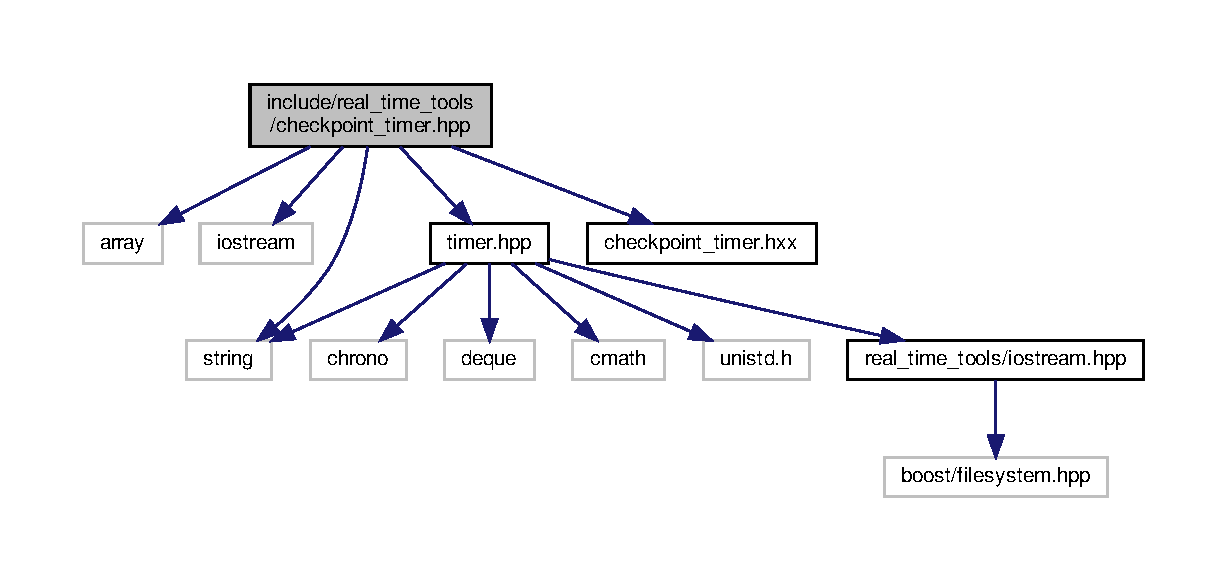
\includegraphics[width=350pt]{checkpoint__timer_8hpp__incl}
\end{center}
\end{figure}
This graph shows which files directly or indirectly include this file\+:
\nopagebreak
\begin{figure}[H]
\begin{center}
\leavevmode
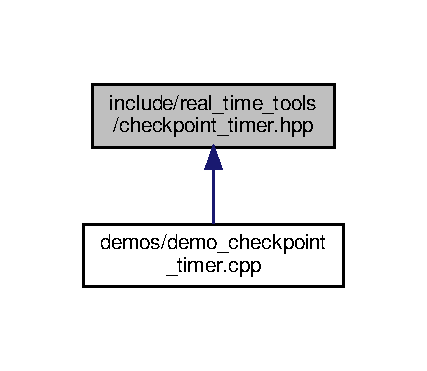
\includegraphics[width=205pt]{checkpoint__timer_8hpp__dep__incl}
\end{center}
\end{figure}
\subsection*{Classes}
\begin{DoxyCompactItemize}
\item 
class \hyperlink{classreal__time__tools_1_1CheckpointTimer}{real\+\_\+time\+\_\+tools\+::\+Checkpoint\+Timer$<$ N\+U\+M\+\_\+\+C\+H\+E\+C\+K\+P\+O\+I\+N\+T\+S, E\+N\+A\+B\+L\+E\+D $>$}
\begin{DoxyCompactList}\small\item\em \hyperlink{classreal__time__tools_1_1Timer}{Timer} to measure code execution time with \char`\"{}checkpoints\char`\"{}. \end{DoxyCompactList}\end{DoxyCompactItemize}


\subsection{Detailed Description}
Implementation of the Checkpoint\+Timer class. 

\begin{DoxyRefDesc}{License}
\item[\hyperlink{license__license000002}{License}]B\+SD 3-\/clause \end{DoxyRefDesc}
\begin{DoxyCopyright}{Copyright}
Copyright (c) 2020, New York University and Max Planck Gesellschaft 
\end{DoxyCopyright}

\hypertarget{checkpoint__timer_8hxx}{}\section{include/real\+\_\+time\+\_\+tools/checkpoint\+\_\+timer.hxx File Reference}
\label{checkpoint__timer_8hxx}\index{include/real\+\_\+time\+\_\+tools/checkpoint\+\_\+timer.\+hxx@{include/real\+\_\+time\+\_\+tools/checkpoint\+\_\+timer.\+hxx}}


Implementation of the Checkpoint\+Timer class.  


This graph shows which files directly or indirectly include this file\+:
\nopagebreak
\begin{figure}[H]
\begin{center}
\leavevmode
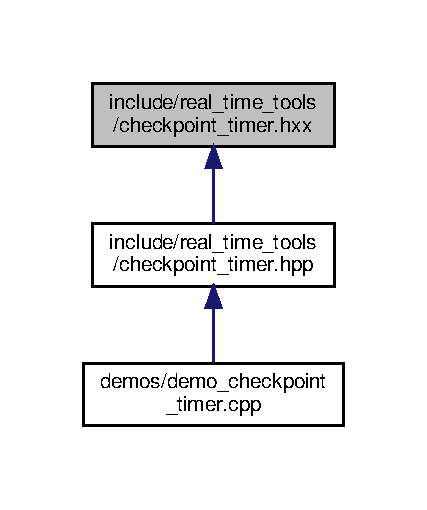
\includegraphics[width=205pt]{checkpoint__timer_8hxx__dep__incl}
\end{center}
\end{figure}


\subsection{Detailed Description}
Implementation of the Checkpoint\+Timer class. 

\begin{DoxyRefDesc}{License}
\item[\hyperlink{license__license000003}{License}]B\+SD 3-\/clause \end{DoxyRefDesc}
\begin{DoxyCopyright}{Copyright}
Copyright (c) 2020, New York University and Max Planck Gesellschaft
\end{DoxyCopyright}
\begin{DoxyRefDesc}{License}
\item[\hyperlink{license__license000004}{License}]B\+SD 3-\/clause \end{DoxyRefDesc}
\begin{DoxyCopyright}{Copyright}
Copyright (c) 2020, New York University and Max Planck Gesellschaft 
\end{DoxyCopyright}

\hypertarget{frequency__manager_8hpp}{}\section{include/real\+\_\+time\+\_\+tools/frequency\+\_\+manager.hpp File Reference}
\label{frequency__manager_8hpp}\index{include/real\+\_\+time\+\_\+tools/frequency\+\_\+manager.\+hpp@{include/real\+\_\+time\+\_\+tools/frequency\+\_\+manager.\+hpp}}


Tools for enforcing a desired frequency in a loop.  


{\ttfamily \#include \char`\"{}real\+\_\+time\+\_\+tools/timer.\+hpp\char`\"{}}\newline
Include dependency graph for frequency\+\_\+manager.\+hpp\+:
\nopagebreak
\begin{figure}[H]
\begin{center}
\leavevmode
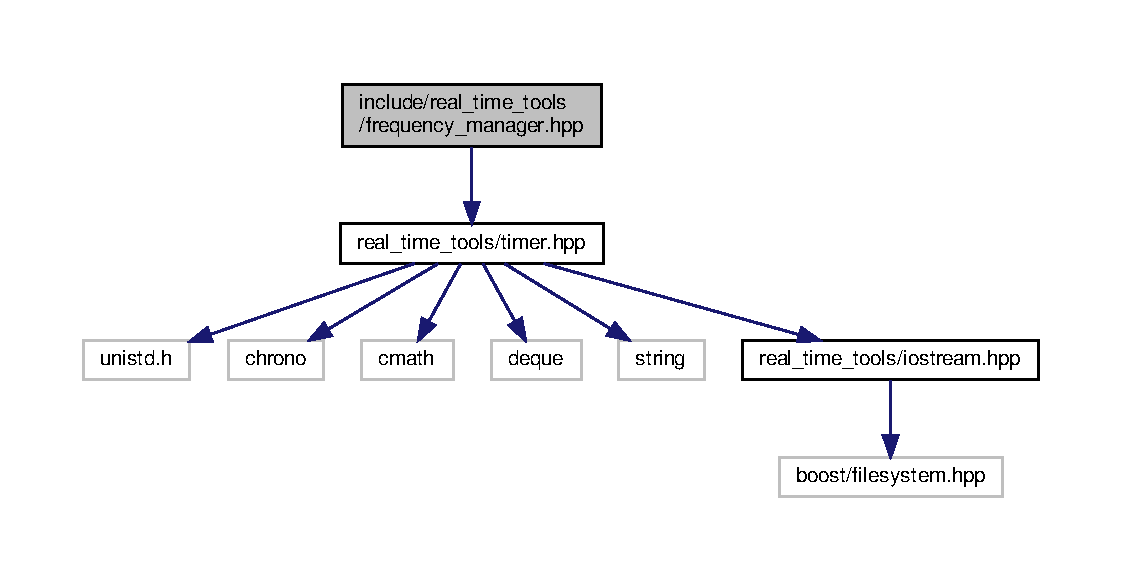
\includegraphics[width=350pt]{frequency__manager_8hpp__incl}
\end{center}
\end{figure}
\subsection*{Classes}
\begin{DoxyCompactItemize}
\item 
class \hyperlink{classreal__time__tools_1_1FrequencyManager}{real\+\_\+time\+\_\+tools\+::\+Frequency\+Manager}
\begin{DoxyCompactList}\small\item\em Class to have threads / loops running at a desired frequency. \end{DoxyCompactList}\end{DoxyCompactItemize}


\subsection{Detailed Description}
Tools for enforcing a desired frequency in a loop. 

\begin{DoxyAuthor}{Author}
Vincent Berenz (\href{mailto:vberenz@tue.mpg.de}{\tt vberenz@tue.\+mpg.\+de}) license License B\+S\+D-\/3-\/\+Clause 
\end{DoxyAuthor}
\begin{DoxyCopyright}{Copyright}
Copyright (c) 2019, New York University and Max Planck Gesellschaft. 
\end{DoxyCopyright}
\begin{DoxyDate}{Date}
2020-\/03-\/22 
\end{DoxyDate}

\hypertarget{iostream_8hpp}{}\section{include/real\+\_\+time\+\_\+tools/iostream.hpp File Reference}
\label{iostream_8hpp}\index{include/real\+\_\+time\+\_\+tools/iostream.\+hpp@{include/real\+\_\+time\+\_\+tools/iostream.\+hpp}}


Tools for console message display.  


{\ttfamily \#include $<$boost/filesystem.\+hpp$>$}\\*
Include dependency graph for iostream.\+hpp\+:
\nopagebreak
\begin{figure}[H]
\begin{center}
\leavevmode
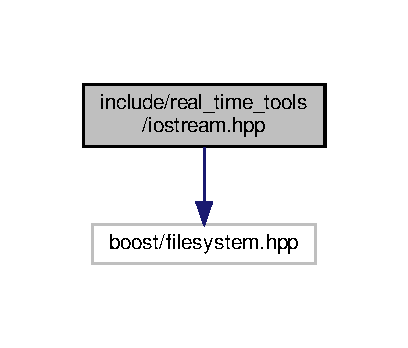
\includegraphics[width=196pt]{iostream_8hpp__incl}
\end{center}
\end{figure}
This graph shows which files directly or indirectly include this file\+:
\nopagebreak
\begin{figure}[H]
\begin{center}
\leavevmode
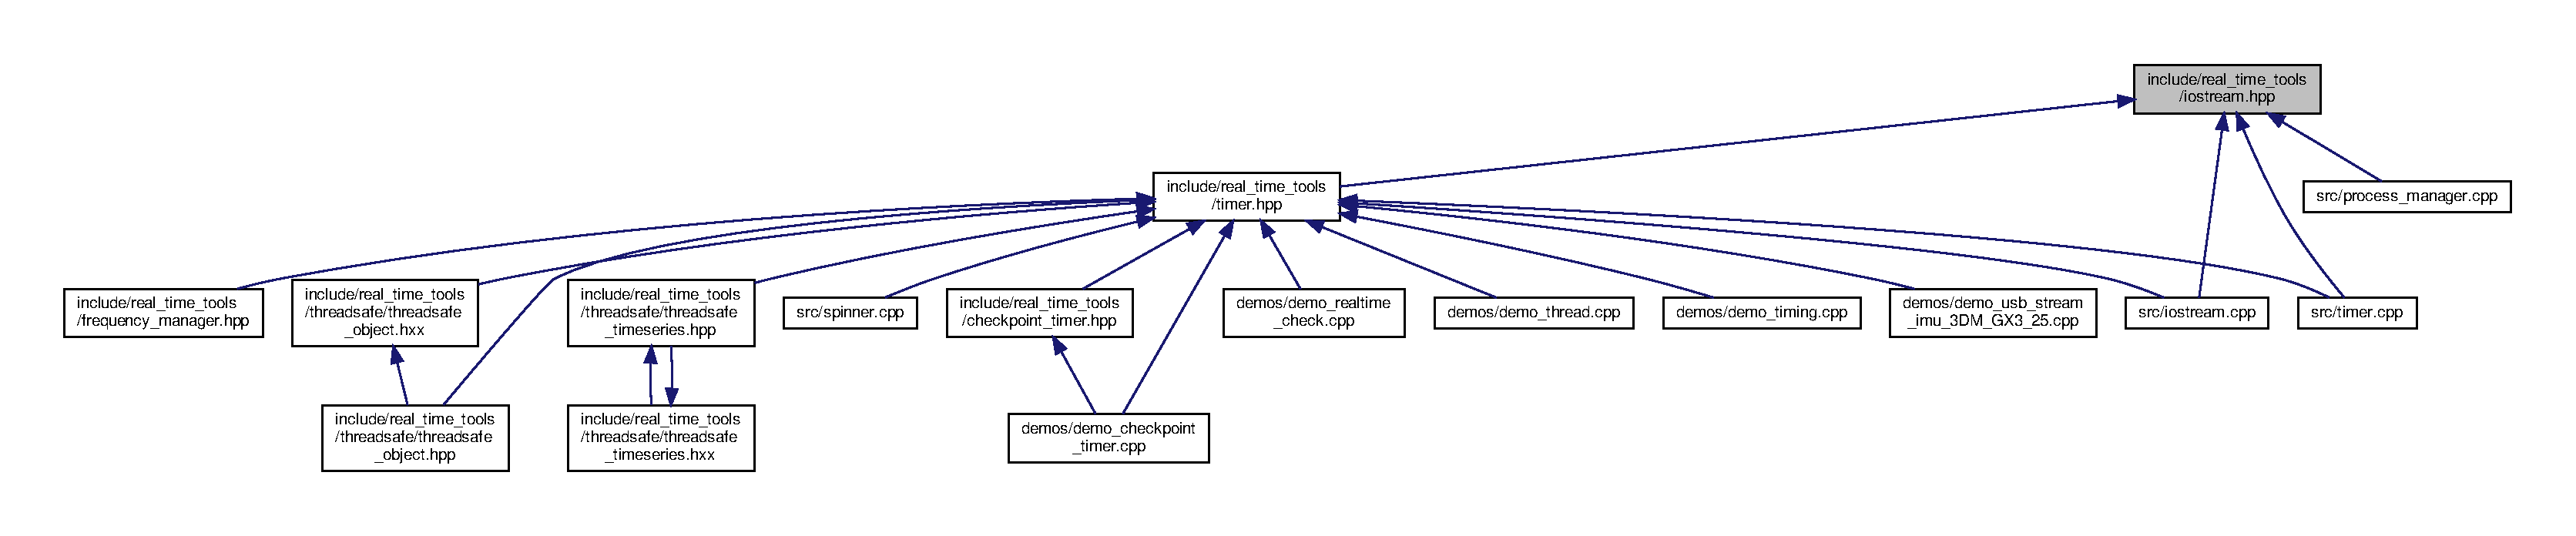
\includegraphics[width=350pt]{iostream_8hpp__dep__incl}
\end{center}
\end{figure}
\subsection*{Functions}
\begin{DoxyCompactItemize}
\item 
std\+::string \hyperlink{iostream_8hpp_a5146f16f97588edcc7dbe28641f4a1fd}{real\+\_\+time\+\_\+tools\+::get\+\_\+log\+\_\+dir} (std\+::string app\+\_\+name)
\begin{DoxyCompactList}\small\item\em Get the logging directory based on a specific application. \end{DoxyCompactList}\item 
bool \hyperlink{iostream_8hpp_a4ce01145e1d43fc6f54c3f654de5bd7d}{real\+\_\+time\+\_\+tools\+::create\+\_\+directory} (std\+::string path)
\begin{DoxyCompactList}\small\item\em Create a directory. \end{DoxyCompactList}\item 
std\+::string \hyperlink{iostream_8hpp_a21f87296dd11ab3784e7b793033a21ed}{real\+\_\+time\+\_\+tools\+::get\+\_\+home\+\_\+dir} ()
\begin{DoxyCompactList}\small\item\em Get the home directory path. \end{DoxyCompactList}\end{DoxyCompactItemize}


\subsection{Detailed Description}
Tools for console message display. 

\begin{DoxyAuthor}{Author}
Maximilien Naveau (\href{mailto:maximilien.naveau@gmail.com}{\tt maximilien.\+naveau@gmail.\+com}) license License B\+S\+D-\/3-\/\+Clause 
\end{DoxyAuthor}
\begin{DoxyCopyright}{Copyright}
Copyright (c) 2019, New York University and Max Planck Gesellschaft. 
\end{DoxyCopyright}
\begin{DoxyDate}{Date}
2019-\/05-\/22 
\end{DoxyDate}


\subsection{Function Documentation}
\index{iostream.\+hpp@{iostream.\+hpp}!create\+\_\+directory@{create\+\_\+directory}}
\index{create\+\_\+directory@{create\+\_\+directory}!iostream.\+hpp@{iostream.\+hpp}}
\subsubsection[{\texorpdfstring{create\+\_\+directory(std\+::string path)}{create_directory(std::string path)}}]{\setlength{\rightskip}{0pt plus 5cm}bool real\+\_\+time\+\_\+tools\+::create\+\_\+directory (
\begin{DoxyParamCaption}
\item[{std\+::string}]{path}
\end{DoxyParamCaption}
)}\hypertarget{iostream_8hpp_file_a4ce01145e1d43fc6f54c3f654de5bd7d}{}\label{iostream_8hpp_file_a4ce01145e1d43fc6f54c3f654de5bd7d}


Create a directory. 


\begin{DoxyParams}{Parameters}
{\em path} & is the path to be created \\
\hline
\end{DoxyParams}
\begin{DoxyReturn}{Returns}
true if everything went well 

false if a problem occur 
\end{DoxyReturn}
\index{iostream.\+hpp@{iostream.\+hpp}!get\+\_\+home\+\_\+dir@{get\+\_\+home\+\_\+dir}}
\index{get\+\_\+home\+\_\+dir@{get\+\_\+home\+\_\+dir}!iostream.\+hpp@{iostream.\+hpp}}
\subsubsection[{\texorpdfstring{get\+\_\+home\+\_\+dir()}{get_home_dir()}}]{\setlength{\rightskip}{0pt plus 5cm}std\+::string real\+\_\+time\+\_\+tools\+::get\+\_\+home\+\_\+dir (
\begin{DoxyParamCaption}
{}
\end{DoxyParamCaption}
)}\hypertarget{iostream_8hpp_file_a21f87296dd11ab3784e7b793033a21ed}{}\label{iostream_8hpp_file_a21f87296dd11ab3784e7b793033a21ed}


Get the home directory path. 

\begin{DoxyReturn}{Returns}
std\+::string the home directory absolute path ending with a \char`\"{}/\char`\"{} 
\end{DoxyReturn}
\index{iostream.\+hpp@{iostream.\+hpp}!get\+\_\+log\+\_\+dir@{get\+\_\+log\+\_\+dir}}
\index{get\+\_\+log\+\_\+dir@{get\+\_\+log\+\_\+dir}!iostream.\+hpp@{iostream.\+hpp}}
\subsubsection[{\texorpdfstring{get\+\_\+log\+\_\+dir(std\+::string app\+\_\+name)}{get_log_dir(std::string app_name)}}]{\setlength{\rightskip}{0pt plus 5cm}std\+::string real\+\_\+time\+\_\+tools\+::get\+\_\+log\+\_\+dir (
\begin{DoxyParamCaption}
\item[{std\+::string}]{app\+\_\+name}
\end{DoxyParamCaption}
)}\hypertarget{iostream_8hpp_file_a5146f16f97588edcc7dbe28641f4a1fd}{}\label{iostream_8hpp_file_a5146f16f97588edcc7dbe28641f4a1fd}


Get the logging directory based on a specific application. 

It creates a direction in \$\+H\+O\+ME/app\+\_\+name/\+Y\+E\+A\+R\+\_\+\+M\+O\+N\+T\+H\+\_\+\+D\+A\+Y\+\_\+\+H\+O\+U\+R\+\_\+\+S\+E\+C\+O\+N\+D/ and return the absolute path of this. It allows the user to dump data in different folders everytime the user launch the application.


\begin{DoxyParams}{Parameters}
{\em app\+\_\+name} & is the application name \\
\hline
\end{DoxyParams}
\begin{DoxyReturn}{Returns}
std\+::string the absolute path to the log directory 
\end{DoxyReturn}

\hypertarget{mutex_8hpp}{}\section{include/real\+\_\+time\+\_\+tools/mutex.hpp File Reference}
\label{mutex_8hpp}\index{include/real\+\_\+time\+\_\+tools/mutex.\+hpp@{include/real\+\_\+time\+\_\+tools/mutex.\+hpp}}


This file implements a real time safe mutex with the dedicated libraries. The A\+PI tries to fit the std A\+PI as much as possible.  


{\ttfamily \#include $<$string$>$}\newline
{\ttfamily \#include $<$mutex$>$}\newline
{\ttfamily \#include $<$condition\+\_\+variable$>$}\newline
Include dependency graph for mutex.\+hpp\+:
\nopagebreak
\begin{figure}[H]
\begin{center}
\leavevmode
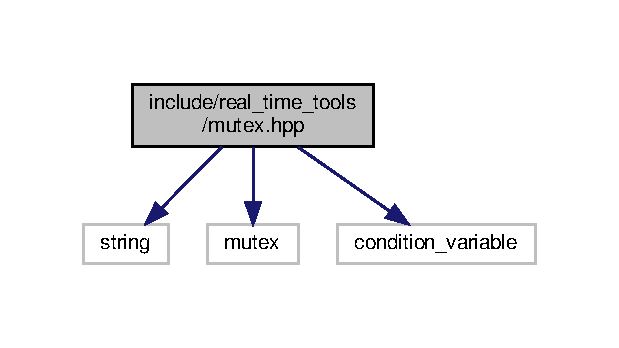
\includegraphics[width=297pt]{mutex_8hpp__incl}
\end{center}
\end{figure}
\subsection*{Classes}
\begin{DoxyCompactItemize}
\item 
class \hyperlink{classreal__time__tools_1_1RealTimeMutex}{real\+\_\+time\+\_\+tools\+::\+Real\+Time\+Mutex}
\begin{DoxyCompactList}\small\item\em This class uses the real-\/time A\+PI of xenomai and posix to implement mutexes. \end{DoxyCompactList}\end{DoxyCompactItemize}
\subsection*{Macros}
\begin{DoxyCompactItemize}
\item 
\mbox{\Hypertarget{mutex_8hpp_a1acf1ce04ab7fe3a5972c0618adcbbac}\label{mutex_8hpp_a1acf1ce04ab7fe3a5972c0618adcbbac}} 
\#define {\bfseries rt\+\_\+printf}~printf
\end{DoxyCompactItemize}
\subsection*{Typedefs}
\begin{DoxyCompactItemize}
\item 
\mbox{\Hypertarget{mutex_8hpp_a1ddc3c11c7ede92bbf52bafb61009ba2}\label{mutex_8hpp_a1ddc3c11c7ede92bbf52bafb61009ba2}} 
typedef std\+::mutex $\ast$ \hyperlink{mutex_8hpp_a1ddc3c11c7ede92bbf52bafb61009ba2}{real\+\_\+time\+\_\+tools\+::\+Real\+Time\+Mutex\+\_\+t}
\begin{DoxyCompactList}\small\item\em Alias for the real time mutex. \end{DoxyCompactList}\item 
\mbox{\Hypertarget{mutex_8hpp_a8a363a3ca3b0f37f2fd06ae393e871bb}\label{mutex_8hpp_a8a363a3ca3b0f37f2fd06ae393e871bb}} 
typedef std\+::condition\+\_\+variable \hyperlink{mutex_8hpp_a8a363a3ca3b0f37f2fd06ae393e871bb}{real\+\_\+time\+\_\+tools\+::rt\+\_\+cond}
\begin{DoxyCompactList}\small\item\em Alias for the real time condition variable. \end{DoxyCompactList}\end{DoxyCompactItemize}


\subsection{Detailed Description}
This file implements a real time safe mutex with the dedicated libraries. The A\+PI tries to fit the std A\+PI as much as possible. 

\begin{DoxyAuthor}{Author}
Maximilien Naveau license License B\+S\+D-\/3-\/\+Clause 
\end{DoxyAuthor}
\begin{DoxyCopyright}{Copyright}
Copyright (c) 2019, New York University and Max Planck Gesellschaft. 
\end{DoxyCopyright}
\begin{DoxyDate}{Date}
2019-\/11-\/19 
\end{DoxyDate}

\hypertarget{process__manager_8hpp}{}\section{include/real\+\_\+time\+\_\+tools/process\+\_\+manager.hpp File Reference}
\label{process__manager_8hpp}\index{include/real\+\_\+time\+\_\+tools/process\+\_\+manager.\+hpp@{include/real\+\_\+time\+\_\+tools/process\+\_\+manager.\+hpp}}


Tools to fix the C\+PU to specific processor.  


{\ttfamily \#include $<$vector$>$}\newline
Include dependency graph for process\+\_\+manager.\+hpp\+:
\nopagebreak
\begin{figure}[H]
\begin{center}
\leavevmode
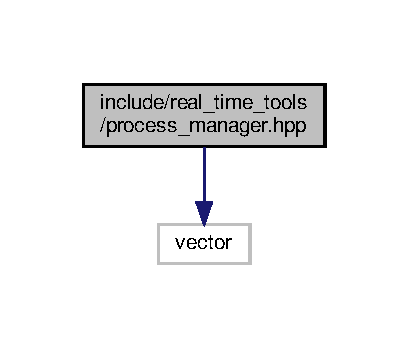
\includegraphics[width=196pt]{process__manager_8hpp__incl}
\end{center}
\end{figure}
This graph shows which files directly or indirectly include this file\+:
\nopagebreak
\begin{figure}[H]
\begin{center}
\leavevmode
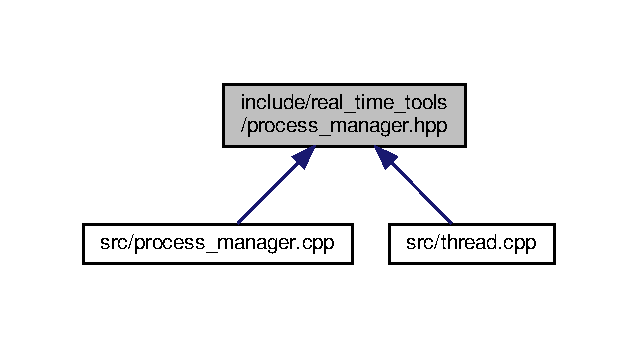
\includegraphics[width=306pt]{process__manager_8hpp__dep__incl}
\end{center}
\end{figure}
\subsection*{Functions}
\begin{DoxyCompactItemize}
\item 
bool \hyperlink{process__manager_8hpp_ae4959078e00ed85dd26b9a96dcd8fd3b}{real\+\_\+time\+\_\+tools\+::fix\+\_\+current\+\_\+process\+\_\+to\+\_\+cpu} (std\+::vector$<$ int $>$ \&cpu\+\_\+affinities, int pid)
\begin{DoxyCompactList}\small\item\em Pin an executing process to a specific C\+PU in order to avoid jumps between C\+P\+Us. \end{DoxyCompactList}\item 
bool \hyperlink{process__manager_8hpp_a6a8ceffef6761ee22e436a1151f020af}{real\+\_\+time\+\_\+tools\+::set\+\_\+cpu\+\_\+dma\+\_\+latency} (int max\+\_\+latency\+\_\+us)
\begin{DoxyCompactList}\small\item\em Set the \+\_\+cpu\+\_\+dma\+\_\+latency object\+We can set the maximum C\+PU latency for processes in micro seconds. \end{DoxyCompactList}\end{DoxyCompactItemize}


\subsection{Detailed Description}
Tools to fix the C\+PU to specific processor. 

\begin{DoxyAuthor}{Author}
Maximilien Naveau (\href{mailto:maximilien.naveau@gmail.com}{\tt maximilien.\+naveau@gmail.\+com}) 
\end{DoxyAuthor}
\begin{DoxyCopyright}{Copyright}
Copyright (c) 2019, New York University and Max Planck Gesellschaft. 
\end{DoxyCopyright}
\begin{DoxyDate}{Date}
2019-\/05-\/06 
\end{DoxyDate}


\subsection{Function Documentation}
\mbox{\Hypertarget{process__manager_8hpp_file_ae4959078e00ed85dd26b9a96dcd8fd3b}\label{process__manager_8hpp_file_ae4959078e00ed85dd26b9a96dcd8fd3b}} 
\index{process\+\_\+manager.\+hpp@{process\+\_\+manager.\+hpp}!fix\+\_\+current\+\_\+process\+\_\+to\+\_\+cpu@{fix\+\_\+current\+\_\+process\+\_\+to\+\_\+cpu}}
\index{fix\+\_\+current\+\_\+process\+\_\+to\+\_\+cpu@{fix\+\_\+current\+\_\+process\+\_\+to\+\_\+cpu}!process\+\_\+manager.\+hpp@{process\+\_\+manager.\+hpp}}
\subsubsection{\texorpdfstring{fix\+\_\+current\+\_\+process\+\_\+to\+\_\+cpu()}{fix\_current\_process\_to\_cpu()}}
{\footnotesize\ttfamily bool real\+\_\+time\+\_\+tools\+::fix\+\_\+current\+\_\+process\+\_\+to\+\_\+cpu (\begin{DoxyParamCaption}\item[{std\+::vector$<$ int $>$ \&}]{cpu\+\_\+affinities,  }\item[{int}]{pid }\end{DoxyParamCaption})}



Pin an executing process to a specific C\+PU in order to avoid jumps between C\+P\+Us. 


\begin{DoxyParams}{Parameters}
{\em cpu\+\_\+affinities} & is the index of the C\+PU one wants to pin the process on. \\
\hline
{\em pid} & is the P\+ID of the current process. \\
\hline
\end{DoxyParams}
\begin{DoxyReturn}{Returns}
true if everything went well. 

false otherwise 
\end{DoxyReturn}
\mbox{\Hypertarget{process__manager_8hpp_file_a6a8ceffef6761ee22e436a1151f020af}\label{process__manager_8hpp_file_a6a8ceffef6761ee22e436a1151f020af}} 
\index{process\+\_\+manager.\+hpp@{process\+\_\+manager.\+hpp}!set\+\_\+cpu\+\_\+dma\+\_\+latency@{set\+\_\+cpu\+\_\+dma\+\_\+latency}}
\index{set\+\_\+cpu\+\_\+dma\+\_\+latency@{set\+\_\+cpu\+\_\+dma\+\_\+latency}!process\+\_\+manager.\+hpp@{process\+\_\+manager.\+hpp}}
\subsubsection{\texorpdfstring{set\+\_\+cpu\+\_\+dma\+\_\+latency()}{set\_cpu\_dma\_latency()}}
{\footnotesize\ttfamily bool real\+\_\+time\+\_\+tools\+::set\+\_\+cpu\+\_\+dma\+\_\+latency (\begin{DoxyParamCaption}\item[{int}]{max\+\_\+latency\+\_\+us }\end{DoxyParamCaption})}



Set the \+\_\+cpu\+\_\+dma\+\_\+latency object\+We can set the maximum C\+PU latency for processes in micro seconds. 


\begin{DoxyParams}{Parameters}
{\em max\+\_\+latency\+\_\+us} & is the maximum latency in micro-\/seconds. \\
\hline
\end{DoxyParams}
\begin{DoxyReturn}{Returns}
true if everything went well. 

false if something went wrong. 
\end{DoxyReturn}

\hypertarget{realtime__check_8hpp}{}\section{include/real\+\_\+time\+\_\+tools/realtime\+\_\+check.hpp File Reference}
\label{realtime__check_8hpp}\index{include/real\+\_\+time\+\_\+tools/realtime\+\_\+check.\+hpp@{include/real\+\_\+time\+\_\+tools/realtime\+\_\+check.\+hpp}}


Tools for checking the real time of an algorithm.  


{\ttfamily \#include $<$math.\+h$>$}\newline
{\ttfamily \#include $<$chrono$>$}\newline
{\ttfamily \#include $<$iostream$>$}\newline
{\ttfamily \#include $<$limits$>$}\newline
{\ttfamily \#include $<$mutex$>$}\newline
Include dependency graph for realtime\+\_\+check.\+hpp\+:
\nopagebreak
\begin{figure}[H]
\begin{center}
\leavevmode
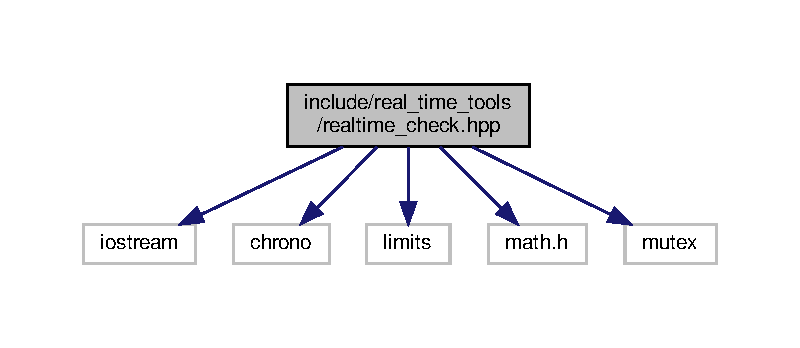
\includegraphics[width=350pt]{realtime__check_8hpp__incl}
\end{center}
\end{figure}
This graph shows which files directly or indirectly include this file\+:
\nopagebreak
\begin{figure}[H]
\begin{center}
\leavevmode
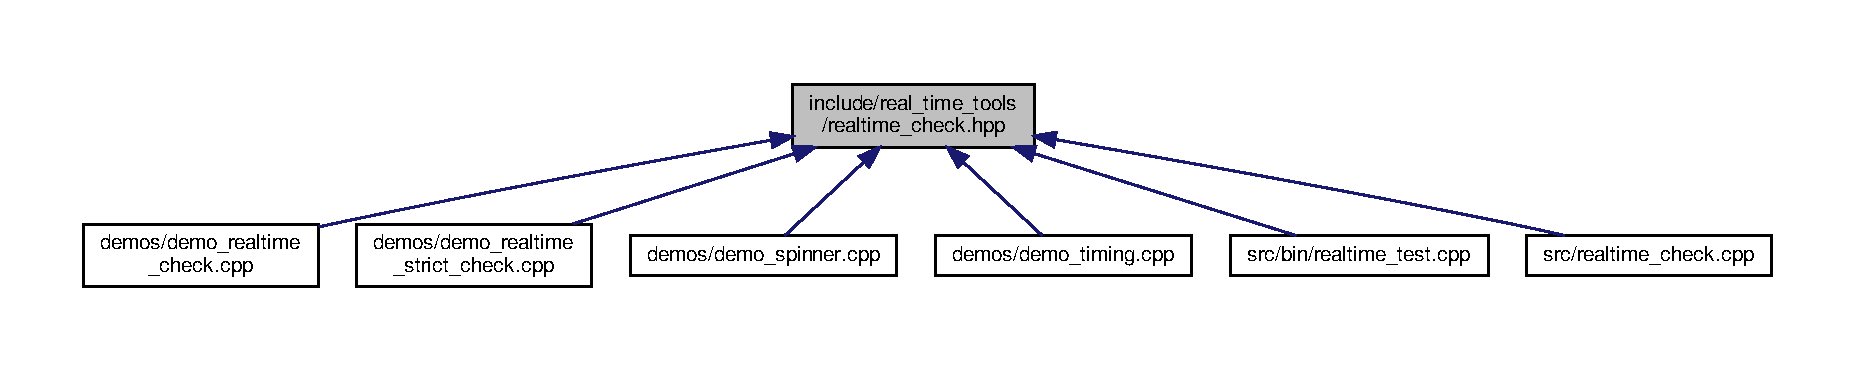
\includegraphics[width=350pt]{realtime__check_8hpp__dep__incl}
\end{center}
\end{figure}
\subsection*{Classes}
\begin{DoxyCompactItemize}
\item 
class \hyperlink{classreal__time__tools_1_1RealTimeCheck}{real\+\_\+time\+\_\+tools\+::\+Real\+Time\+Check}
\begin{DoxyCompactList}\small\item\em super simple class for checking if thread ever lost realtime. \end{DoxyCompactList}\end{DoxyCompactItemize}


\subsection{Detailed Description}
Tools for checking the real time of an algorithm. 

\begin{DoxyAuthor}{Author}
Maximilien Naveau (\href{mailto:maximilien.naveau@gmail.com}{\tt maximilien.\+naveau@gmail.\+com}) license License B\+S\+D-\/3-\/\+Clause 
\end{DoxyAuthor}
\begin{DoxyCopyright}{Copyright}
Copyright (c) 2019, New York University and Max Planck Gesellschaft. 
\end{DoxyCopyright}
\begin{DoxyDate}{Date}
2019-\/05-\/22 
\end{DoxyDate}

\hypertarget{rt__mutex_8hpp}{}\section{include/real\+\_\+time\+\_\+tools/rt\+\_\+mutex.hpp File Reference}
\label{rt__mutex_8hpp}\index{include/real\+\_\+time\+\_\+tools/rt\+\_\+mutex.\+hpp@{include/real\+\_\+time\+\_\+tools/rt\+\_\+mutex.\+hpp}}


Expose real time O\+Ss mutex through a common A\+PI.  


{\ttfamily \#include $<$pthread.\+h$>$}\\*
{\ttfamily \#include $<$sys/time.\+h$>$}\\*
Include dependency graph for rt\+\_\+mutex.\+hpp\+:
\nopagebreak
\begin{figure}[H]
\begin{center}
\leavevmode
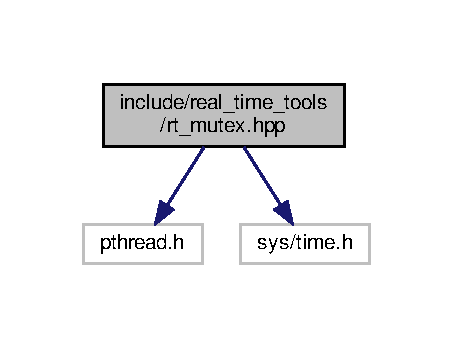
\includegraphics[width=218pt]{rt__mutex_8hpp__incl}
\end{center}
\end{figure}
\subsection*{Typedefs}
\begin{DoxyCompactItemize}
\item 
typedef pthread\+\_\+mutex\+\_\+t \hyperlink{rt__mutex_8hpp_a645c5f8185139f4e3332271edb8690e5}{rt\+\_\+mutex}
\begin{DoxyCompactList}\small\item\em Alias for the real time mutex. \end{DoxyCompactList}\item 
typedef pthread\+\_\+cond\+\_\+t \hyperlink{rt__mutex_8hpp_a668d08f0241c505774e0fac47a16befe}{rt\+\_\+cond}
\begin{DoxyCompactList}\small\item\em Alias for the real time condition variable. \end{DoxyCompactList}\end{DoxyCompactItemize}
\subsection*{Functions}
\begin{DoxyCompactItemize}
\item 
static int \hyperlink{rt__mutex_8hpp_a4d314f52e912dc6b62aae06083f657f0}{rt\+\_\+mutex\+\_\+init} (\hyperlink{rt__mutex_8hpp_a645c5f8185139f4e3332271edb8690e5}{rt\+\_\+mutex} $\ast$mutex)
\begin{DoxyCompactList}\small\item\em Initialize the mutex. \end{DoxyCompactList}\item 
static int \hyperlink{rt__mutex_8hpp_ac16c36f2796d1d2e1707ef29c2e59882}{rt\+\_\+mutex\+\_\+destroy} (\hyperlink{rt__mutex_8hpp_a645c5f8185139f4e3332271edb8690e5}{rt\+\_\+mutex} $\ast$mutex)
\begin{DoxyCompactList}\small\item\em Destroy the mutex. \end{DoxyCompactList}\item 
static int \hyperlink{rt__mutex_8hpp_aeb86d0934fa6ede664749a79b47e8a03}{rt\+\_\+mutex\+\_\+lock} (\hyperlink{rt__mutex_8hpp_a645c5f8185139f4e3332271edb8690e5}{rt\+\_\+mutex} $\ast$mutex)
\begin{DoxyCompactList}\small\item\em Lock the mutex. \end{DoxyCompactList}\item 
static int \hyperlink{rt__mutex_8hpp_abd0f53c90d881554715d2474beedf997}{rt\+\_\+mutex\+\_\+unlock} (\hyperlink{rt__mutex_8hpp_a645c5f8185139f4e3332271edb8690e5}{rt\+\_\+mutex} $\ast$mutex)
\begin{DoxyCompactList}\small\item\em Unlock the mutex. \end{DoxyCompactList}\end{DoxyCompactItemize}


\subsection{Detailed Description}
Expose real time O\+Ss mutex through a common A\+PI. 

\begin{DoxyAuthor}{Author}
Maximilien Naveau (\href{mailto:maximilien.naveau@gmail.com}{\tt maximilien.\+naveau@gmail.\+com}) license License B\+S\+D-\/3-\/\+Clause 
\end{DoxyAuthor}
\begin{DoxyCopyright}{Copyright}
Copyright (c) 2019, New York University and Max Planck Gesellschaft. 
\end{DoxyCopyright}
\begin{DoxyDate}{Date}
2019-\/05-\/22 
\end{DoxyDate}


\subsection{Typedef Documentation}
\index{rt\+\_\+mutex.\+hpp@{rt\+\_\+mutex.\+hpp}!rt\+\_\+cond@{rt\+\_\+cond}}
\index{rt\+\_\+cond@{rt\+\_\+cond}!rt\+\_\+mutex.\+hpp@{rt\+\_\+mutex.\+hpp}}
\subsubsection[{\texorpdfstring{rt\+\_\+cond}{rt_cond}}]{\setlength{\rightskip}{0pt plus 5cm}typedef pthread\+\_\+cond\+\_\+t {\bf rt\+\_\+cond}}\hypertarget{rt__mutex_8hpp_a668d08f0241c505774e0fac47a16befe}{}\label{rt__mutex_8hpp_a668d08f0241c505774e0fac47a16befe}


Alias for the real time condition variable. 

\index{rt\+\_\+mutex.\+hpp@{rt\+\_\+mutex.\+hpp}!rt\+\_\+mutex@{rt\+\_\+mutex}}
\index{rt\+\_\+mutex@{rt\+\_\+mutex}!rt\+\_\+mutex.\+hpp@{rt\+\_\+mutex.\+hpp}}
\subsubsection[{\texorpdfstring{rt\+\_\+mutex}{rt_mutex}}]{\setlength{\rightskip}{0pt plus 5cm}typedef pthread\+\_\+mutex\+\_\+t {\bf rt\+\_\+mutex}}\hypertarget{rt__mutex_8hpp_a645c5f8185139f4e3332271edb8690e5}{}\label{rt__mutex_8hpp_a645c5f8185139f4e3332271edb8690e5}


Alias for the real time mutex. 



\subsection{Function Documentation}
\index{rt\+\_\+mutex.\+hpp@{rt\+\_\+mutex.\+hpp}!rt\+\_\+mutex\+\_\+destroy@{rt\+\_\+mutex\+\_\+destroy}}
\index{rt\+\_\+mutex\+\_\+destroy@{rt\+\_\+mutex\+\_\+destroy}!rt\+\_\+mutex.\+hpp@{rt\+\_\+mutex.\+hpp}}
\subsubsection[{\texorpdfstring{rt\+\_\+mutex\+\_\+destroy(rt\+\_\+mutex $\ast$mutex)}{rt_mutex_destroy(rt_mutex *mutex)}}]{\setlength{\rightskip}{0pt plus 5cm}static int rt\+\_\+mutex\+\_\+destroy (
\begin{DoxyParamCaption}
\item[{{\bf rt\+\_\+mutex} $\ast$}]{mutex}
\end{DoxyParamCaption}
)\hspace{0.3cm}{\ttfamily [inline]}, {\ttfamily [static]}}\hypertarget{rt__mutex_8hpp_ac16c36f2796d1d2e1707ef29c2e59882}{}\label{rt__mutex_8hpp_ac16c36f2796d1d2e1707ef29c2e59882}


Destroy the mutex. 

\index{rt\+\_\+mutex.\+hpp@{rt\+\_\+mutex.\+hpp}!rt\+\_\+mutex\+\_\+init@{rt\+\_\+mutex\+\_\+init}}
\index{rt\+\_\+mutex\+\_\+init@{rt\+\_\+mutex\+\_\+init}!rt\+\_\+mutex.\+hpp@{rt\+\_\+mutex.\+hpp}}
\subsubsection[{\texorpdfstring{rt\+\_\+mutex\+\_\+init(rt\+\_\+mutex $\ast$mutex)}{rt_mutex_init(rt_mutex *mutex)}}]{\setlength{\rightskip}{0pt plus 5cm}static int rt\+\_\+mutex\+\_\+init (
\begin{DoxyParamCaption}
\item[{{\bf rt\+\_\+mutex} $\ast$}]{mutex}
\end{DoxyParamCaption}
)\hspace{0.3cm}{\ttfamily [inline]}, {\ttfamily [static]}}\hypertarget{rt__mutex_8hpp_a4d314f52e912dc6b62aae06083f657f0}{}\label{rt__mutex_8hpp_a4d314f52e912dc6b62aae06083f657f0}


Initialize the mutex. 

\index{rt\+\_\+mutex.\+hpp@{rt\+\_\+mutex.\+hpp}!rt\+\_\+mutex\+\_\+lock@{rt\+\_\+mutex\+\_\+lock}}
\index{rt\+\_\+mutex\+\_\+lock@{rt\+\_\+mutex\+\_\+lock}!rt\+\_\+mutex.\+hpp@{rt\+\_\+mutex.\+hpp}}
\subsubsection[{\texorpdfstring{rt\+\_\+mutex\+\_\+lock(rt\+\_\+mutex $\ast$mutex)}{rt_mutex_lock(rt_mutex *mutex)}}]{\setlength{\rightskip}{0pt plus 5cm}static int rt\+\_\+mutex\+\_\+lock (
\begin{DoxyParamCaption}
\item[{{\bf rt\+\_\+mutex} $\ast$}]{mutex}
\end{DoxyParamCaption}
)\hspace{0.3cm}{\ttfamily [inline]}, {\ttfamily [static]}}\hypertarget{rt__mutex_8hpp_aeb86d0934fa6ede664749a79b47e8a03}{}\label{rt__mutex_8hpp_aeb86d0934fa6ede664749a79b47e8a03}


Lock the mutex. 

\index{rt\+\_\+mutex.\+hpp@{rt\+\_\+mutex.\+hpp}!rt\+\_\+mutex\+\_\+unlock@{rt\+\_\+mutex\+\_\+unlock}}
\index{rt\+\_\+mutex\+\_\+unlock@{rt\+\_\+mutex\+\_\+unlock}!rt\+\_\+mutex.\+hpp@{rt\+\_\+mutex.\+hpp}}
\subsubsection[{\texorpdfstring{rt\+\_\+mutex\+\_\+unlock(rt\+\_\+mutex $\ast$mutex)}{rt_mutex_unlock(rt_mutex *mutex)}}]{\setlength{\rightskip}{0pt plus 5cm}static int rt\+\_\+mutex\+\_\+unlock (
\begin{DoxyParamCaption}
\item[{{\bf rt\+\_\+mutex} $\ast$}]{mutex}
\end{DoxyParamCaption}
)\hspace{0.3cm}{\ttfamily [inline]}, {\ttfamily [static]}}\hypertarget{rt__mutex_8hpp_abd0f53c90d881554715d2474beedf997}{}\label{rt__mutex_8hpp_abd0f53c90d881554715d2474beedf997}


Unlock the mutex. 


\hypertarget{spinner_8hpp}{}\section{include/real\+\_\+time\+\_\+tools/spinner.hpp File Reference}
\label{spinner_8hpp}\index{include/real\+\_\+time\+\_\+tools/spinner.\+hpp@{include/real\+\_\+time\+\_\+tools/spinner.\+hpp}}


Tools for maintaining the timing on a while loop.  


{\ttfamily \#include $<$chrono$>$}\\*
{\ttfamily \#include $<$unistd.\+h$>$}\\*
Include dependency graph for spinner.\+hpp\+:
\nopagebreak
\begin{figure}[H]
\begin{center}
\leavevmode
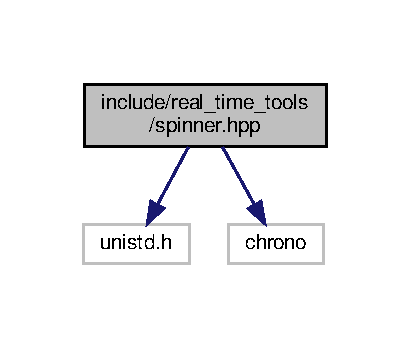
\includegraphics[width=198pt]{spinner_8hpp__incl}
\end{center}
\end{figure}
This graph shows which files directly or indirectly include this file\+:
\nopagebreak
\begin{figure}[H]
\begin{center}
\leavevmode
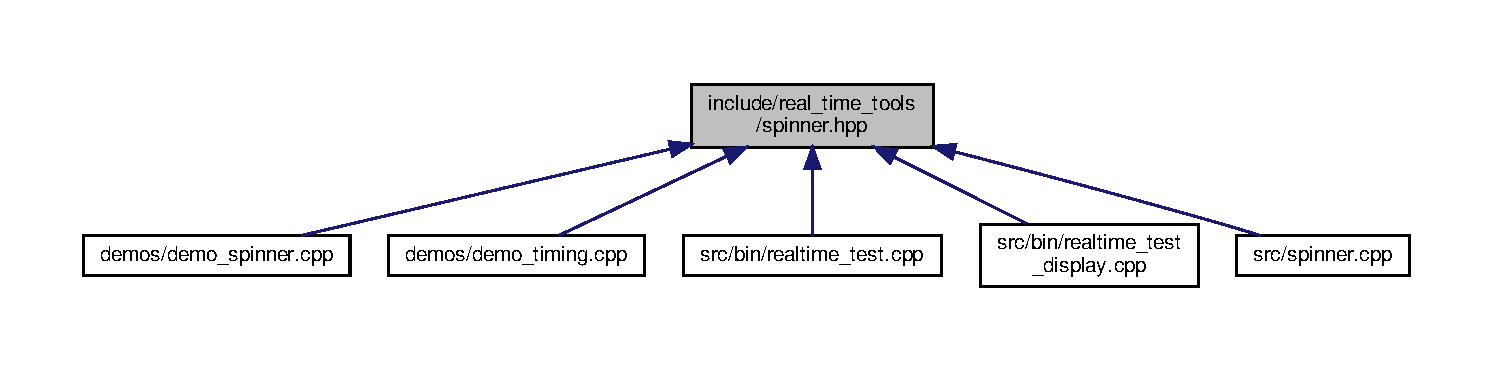
\includegraphics[width=350pt]{spinner_8hpp__dep__incl}
\end{center}
\end{figure}
\subsection*{Classes}
\begin{DoxyCompactItemize}
\item 
class \hyperlink{classreal__time__tools_1_1Spinner}{real\+\_\+time\+\_\+tools\+::\+Spinner}
\begin{DoxyCompactList}\small\item\em Class to have threads / loops running at a desired frequency. \end{DoxyCompactList}\end{DoxyCompactItemize}


\subsection{Detailed Description}
Tools for maintaining the timing on a while loop. 

\begin{DoxyAuthor}{Author}
Maximilien Naveau (\href{mailto:maximilien.naveau@gmail.com}{\tt maximilien.\+naveau@gmail.\+com}) license License B\+S\+D-\/3-\/\+Clause 
\end{DoxyAuthor}
\begin{DoxyCopyright}{Copyright}
Copyright (c) 2019, New York University and Max Planck Gesellschaft. 
\end{DoxyCopyright}
\begin{DoxyDate}{Date}
2019-\/05-\/22 
\end{DoxyDate}

\hypertarget{thread_8hpp}{}\section{include/real\+\_\+time\+\_\+tools/thread.hpp File Reference}
\label{thread_8hpp}\index{include/real\+\_\+time\+\_\+tools/thread.\+hpp@{include/real\+\_\+time\+\_\+tools/thread.\+hpp}}
{\ttfamily \#include $<$string$>$}\newline
{\ttfamily \#include $<$vector$>$}\newline
{\ttfamily \#include $<$memory$>$}\newline
{\ttfamily \#include $<$functional$>$}\newline
Include dependency graph for thread.\+hpp\+:
\nopagebreak
\begin{figure}[H]
\begin{center}
\leavevmode
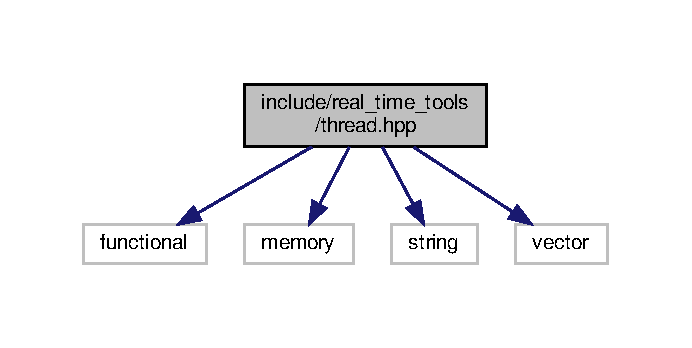
\includegraphics[width=331pt]{thread_8hpp__incl}
\end{center}
\end{figure}
This graph shows which files directly or indirectly include this file\+:
\nopagebreak
\begin{figure}[H]
\begin{center}
\leavevmode
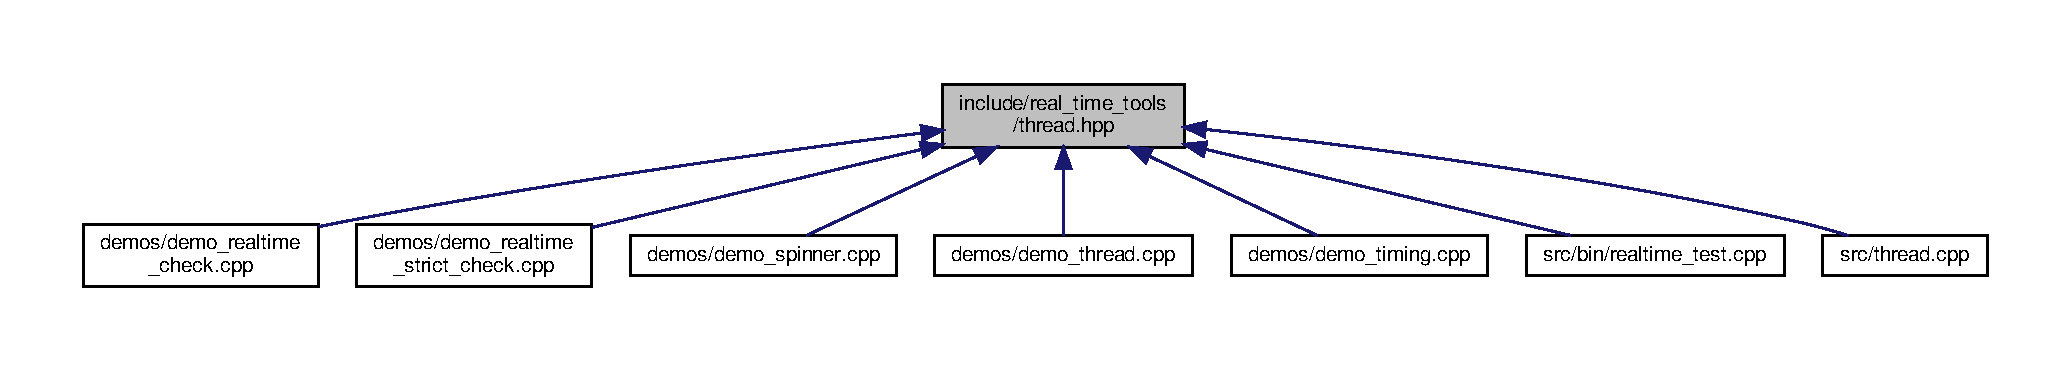
\includegraphics[width=350pt]{thread_8hpp__dep__incl}
\end{center}
\end{figure}
\subsection*{Classes}
\begin{DoxyCompactItemize}
\item 
class \hyperlink{classreal__time__tools_1_1RealTimeThreadParameters}{real\+\_\+time\+\_\+tools\+::\+Real\+Time\+Thread\+Parameters}
\begin{DoxyCompactList}\small\item\em This class is a data structure allowing the user to share configurations among threads. \end{DoxyCompactList}\item 
class \hyperlink{classreal__time__tools_1_1RealTimeThread}{real\+\_\+time\+\_\+tools\+::\+Real\+Time\+Thread}
\begin{DoxyCompactList}\small\item\em This class allows you to spawn thread. \end{DoxyCompactList}\end{DoxyCompactItemize}


\subsection{Detailed Description}
\begin{DoxyAuthor}{Author}
Maximilien Naveau (\href{mailto:mnaveau@tue.mpg.de}{\tt mnaveau@tue.\+mpg.\+de}) license License B\+S\+D-\/3-\/\+Clause 
\end{DoxyAuthor}
\begin{DoxyCopyright}{Copyright}
Copyright (c) 2019, New York University and Max Planck Gesellschaft. 
\end{DoxyCopyright}
\begin{DoxyDate}{Date}
2019-\/11-\/21 
\end{DoxyDate}

\hypertarget{threadsafe__object_8hpp}{}\section{include/real\+\_\+time\+\_\+tools/threadsafe/threadsafe\+\_\+object.hpp File Reference}
\label{threadsafe__object_8hpp}\index{include/real\+\_\+time\+\_\+tools/threadsafe/threadsafe\+\_\+object.\+hpp@{include/real\+\_\+time\+\_\+tools/threadsafe/threadsafe\+\_\+object.\+hpp}}


This file declares templated container for data buffering.  


{\ttfamily \#include $<$array$>$}\newline
{\ttfamily \#include $<$map$>$}\newline
{\ttfamily \#include $<$memory$>$}\newline
{\ttfamily \#include $<$tuple$>$}\newline
{\ttfamily \#include $<$vector$>$}\newline
{\ttfamily \#include \char`\"{}real\+\_\+time\+\_\+tools/timer.\+hpp\char`\"{}}\newline
{\ttfamily \#include $<$condition\+\_\+variable$>$}\newline
{\ttfamily \#include $<$mutex$>$}\newline
{\ttfamily \#include \char`\"{}real\+\_\+time\+\_\+tools/threadsafe/threadsafe\+\_\+object.\+hxx\char`\"{}}\newline
Include dependency graph for threadsafe\+\_\+object.\+hpp\+:
\nopagebreak
\begin{figure}[H]
\begin{center}
\leavevmode
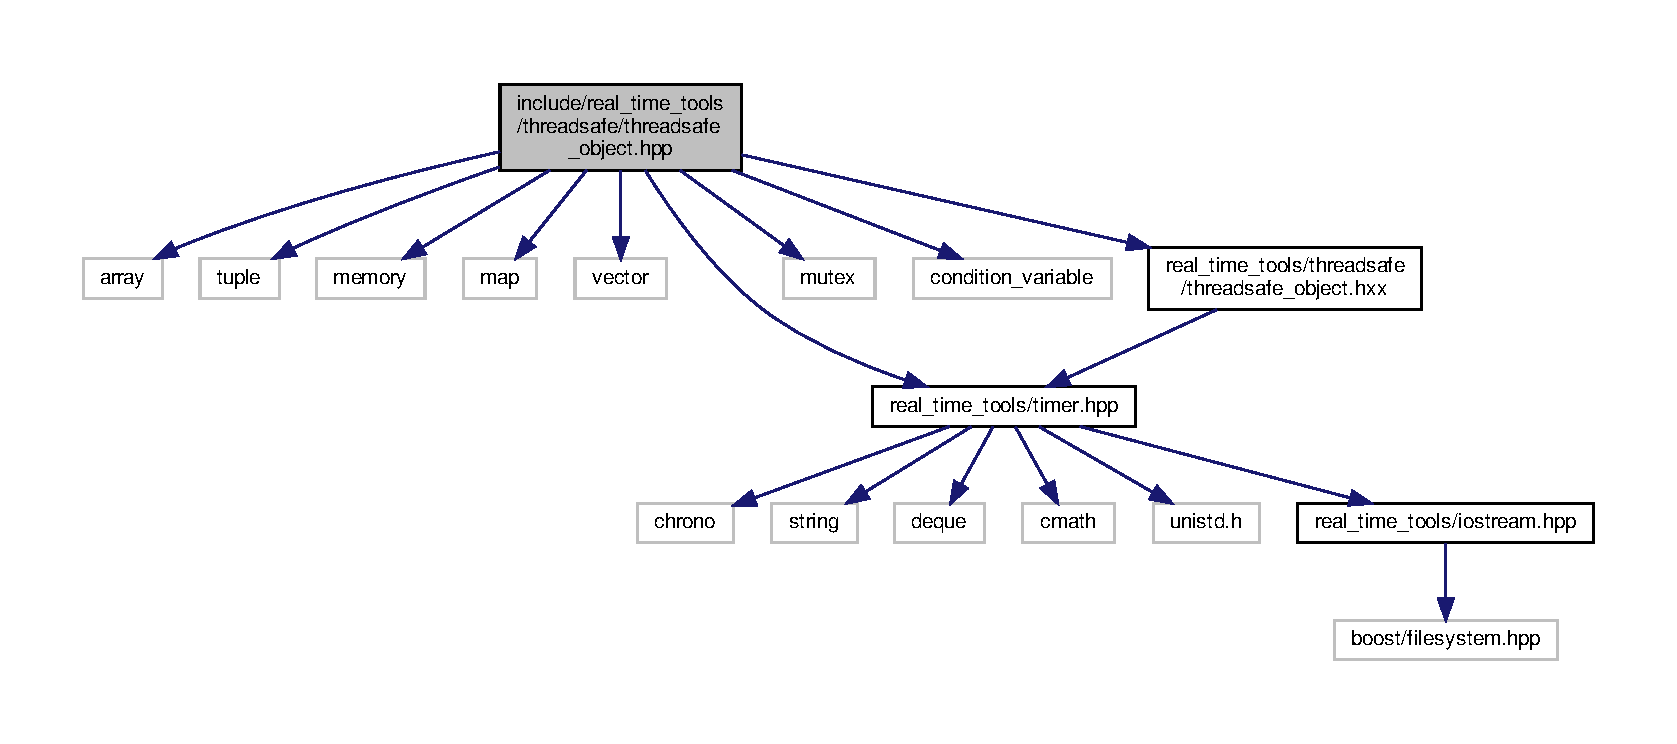
\includegraphics[width=350pt]{threadsafe__object_8hpp__incl}
\end{center}
\end{figure}
\subsection*{Classes}
\begin{DoxyCompactItemize}
\item 
class \hyperlink{classreal__time__tools_1_1ThreadsafeHistoryInterface}{real\+\_\+time\+\_\+tools\+::\+Threadsafe\+History\+Interface$<$ Type $>$}
\begin{DoxyCompactList}\small\item\em This is a template abstract interface class that define a data history. \end{DoxyCompactList}\item 
class \hyperlink{classreal__time__tools_1_1SingletypeThreadsafeObject}{real\+\_\+time\+\_\+tools\+::\+Singletype\+Threadsafe\+Object$<$ Type, S\+I\+Z\+E $>$}
\begin{DoxyCompactList}\small\item\em The \hyperlink{classreal__time__tools_1_1SingletypeThreadsafeObject}{Singletype\+Threadsafe\+Object} is a thread safe object. \end{DoxyCompactList}\item 
class \hyperlink{classreal__time__tools_1_1ThreadsafeObject}{real\+\_\+time\+\_\+tools\+::\+Threadsafe\+Object$<$ Types $>$}
\begin{DoxyCompactList}\small\item\em This object can have several types depending on what ones want to store. \end{DoxyCompactList}\end{DoxyCompactItemize}


\subsection{Detailed Description}
This file declares templated container for data buffering. 

\begin{DoxyAuthor}{Author}
Manuel Wuthrich (\href{mailto:manuel.wuthrich@gmail.com}{\tt manuel.\+wuthrich@gmail.\+com}) 

Maximilien Naveau (\href{mailto:maximilien.naveau@gmail.com}{\tt maximilien.\+naveau@gmail.\+com}) 
\end{DoxyAuthor}
\begin{DoxyVersion}{Version}
0.\+1 
\end{DoxyVersion}
\begin{DoxyDate}{Date}
2018-\/11-\/27
\end{DoxyDate}
\begin{DoxyCopyright}{Copyright}
Copyright (c) 2018 
\end{DoxyCopyright}

\hypertarget{threadsafe__object_8hxx}{}\section{include/real\+\_\+time\+\_\+tools/threadsafe/threadsafe\+\_\+object.hxx File Reference}
\label{threadsafe__object_8hxx}\index{include/real\+\_\+time\+\_\+tools/threadsafe/threadsafe\+\_\+object.\+hxx@{include/real\+\_\+time\+\_\+tools/threadsafe/threadsafe\+\_\+object.\+hxx}}


This file defines the functions from \hyperlink{threadsafe__object_8hpp}{threadsafe\+\_\+object.\+hpp}.  


{\ttfamily \#include \char`\"{}real\+\_\+time\+\_\+tools/timer.\+hpp\char`\"{}}\\*
Include dependency graph for threadsafe\+\_\+object.\+hxx\+:
\nopagebreak
\begin{figure}[H]
\begin{center}
\leavevmode
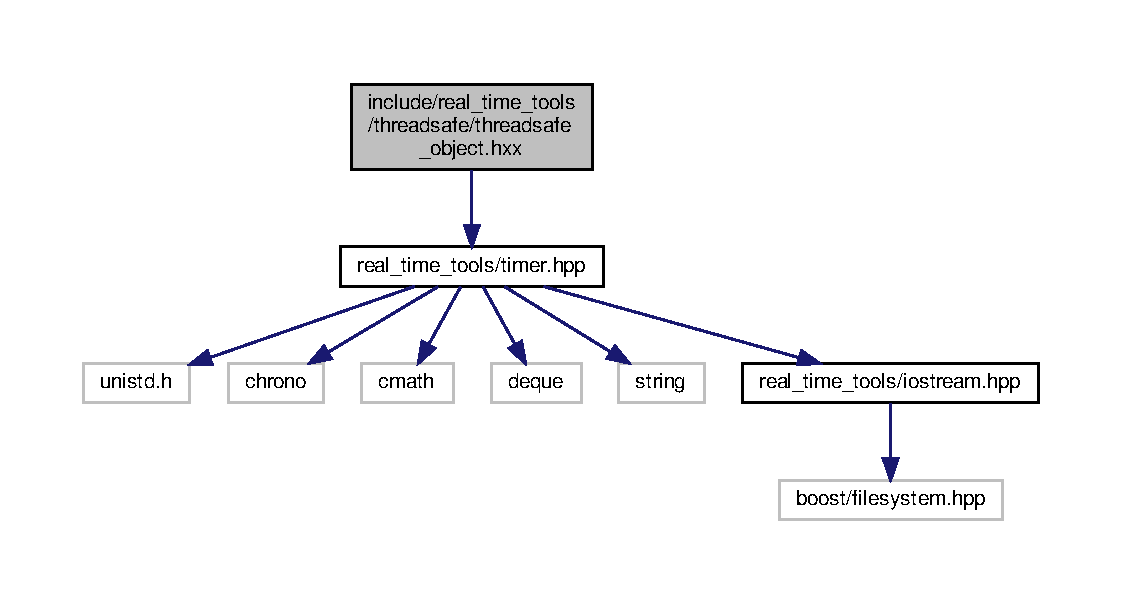
\includegraphics[width=350pt]{threadsafe__object_8hxx__incl}
\end{center}
\end{figure}
This graph shows which files directly or indirectly include this file\+:
\nopagebreak
\begin{figure}[H]
\begin{center}
\leavevmode
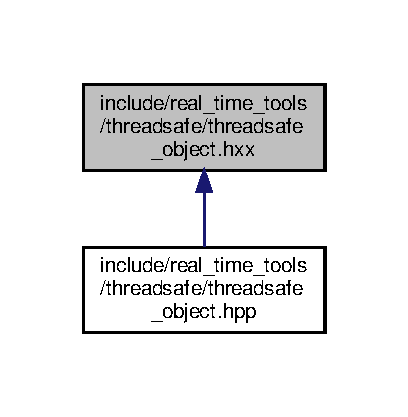
\includegraphics[width=196pt]{threadsafe__object_8hxx__dep__incl}
\end{center}
\end{figure}


\subsection{Detailed Description}
This file defines the functions from \hyperlink{threadsafe__object_8hpp}{threadsafe\+\_\+object.\+hpp}. 

\begin{DoxyAuthor}{Author}
Manuel Wuthrich (\href{mailto:manuel.wuthrich@gmail.com}{\tt manuel.\+wuthrich@gmail.\+com}) 

Maximilien Naveau (\href{mailto:maximilien.naveau@gmail.com}{\tt maximilien.\+naveau@gmail.\+com}) 
\end{DoxyAuthor}
\begin{DoxyVersion}{Version}
0.\+1 
\end{DoxyVersion}
\begin{DoxyDate}{Date}
2018-\/11-\/29
\end{DoxyDate}
\begin{DoxyCopyright}{Copyright}
Copyright (c) 2018 
\end{DoxyCopyright}

\hypertarget{threadsafe__timeseries_8hpp}{}\section{include/real\+\_\+time\+\_\+tools/threadsafe/threadsafe\+\_\+timeseries.hpp File Reference}
\label{threadsafe__timeseries_8hpp}\index{include/real\+\_\+time\+\_\+tools/threadsafe/threadsafe\+\_\+timeseries.\+hpp@{include/real\+\_\+time\+\_\+tools/threadsafe/threadsafe\+\_\+timeseries.\+hpp}}
{\ttfamily \#include $<$memory$>$}\\*
{\ttfamily \#include $<$vector$>$}\\*
{\ttfamily \#include \char`\"{}real\+\_\+time\+\_\+tools/timer.\+hpp\char`\"{}}\\*
{\ttfamily \#include $<$condition\+\_\+variable$>$}\\*
{\ttfamily \#include $<$mutex$>$}\\*
{\ttfamily \#include \char`\"{}real\+\_\+time\+\_\+tools/threadsafe/threadsafe\+\_\+timeseries.\+hxx\char`\"{}}\\*
Include dependency graph for threadsafe\+\_\+timeseries.\+hpp\+:
\nopagebreak
\begin{figure}[H]
\begin{center}
\leavevmode
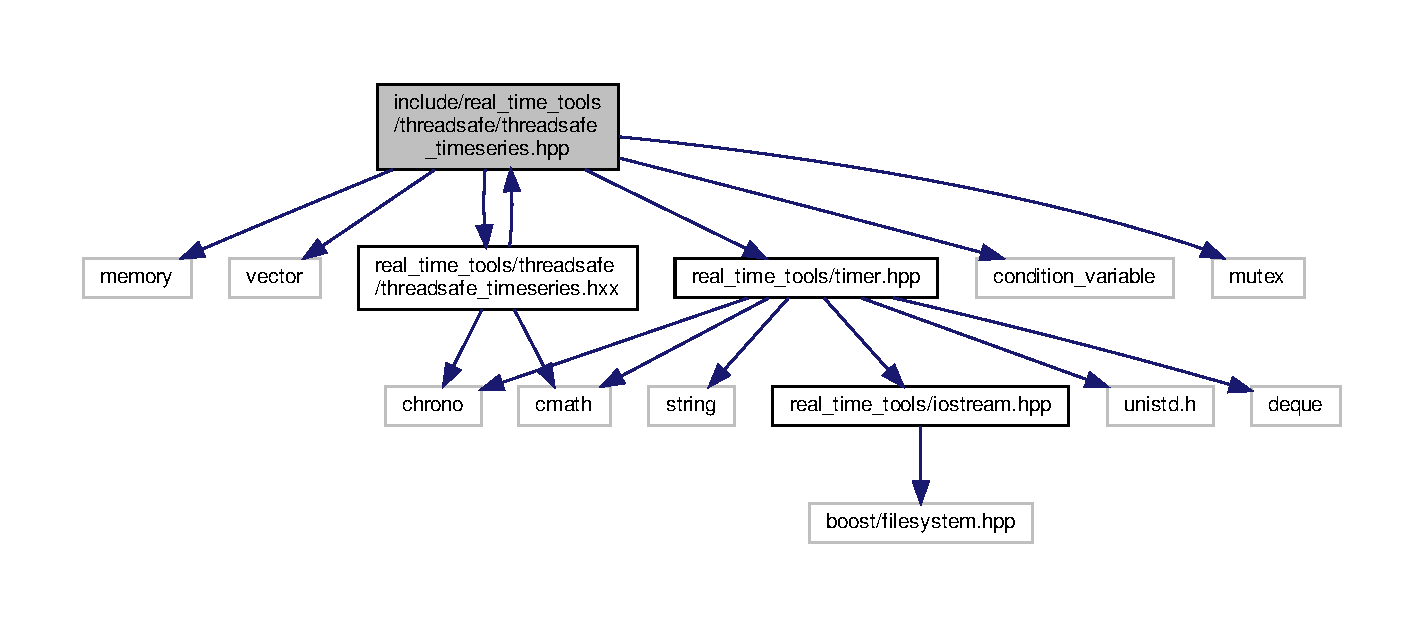
\includegraphics[width=350pt]{threadsafe__timeseries_8hpp__incl}
\end{center}
\end{figure}
This graph shows which files directly or indirectly include this file\+:
\nopagebreak
\begin{figure}[H]
\begin{center}
\leavevmode
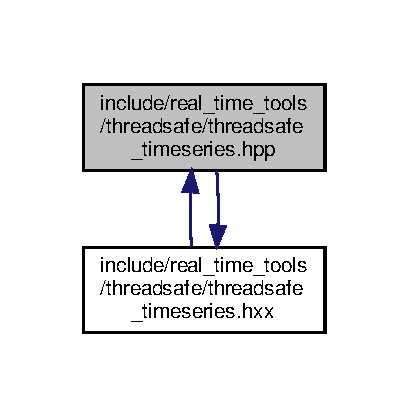
\includegraphics[width=196pt]{threadsafe__timeseries_8hpp__dep__incl}
\end{center}
\end{figure}
\subsection*{Classes}
\begin{DoxyCompactItemize}
\item 
class \hyperlink{classreal__time__tools_1_1ThreadsafeTimeseries}{real\+\_\+time\+\_\+tools\+::\+Threadsafe\+Timeseries$<$ Type $>$}
\begin{DoxyCompactList}\small\item\em implements a timeseries $ X_{{oldest}:{newest}} $ which can safely be accessed from multiple threads. \end{DoxyCompactList}\end{DoxyCompactItemize}


\subsection{Detailed Description}
\begin{DoxyAuthor}{Author}
Manuel Wuthrich (\href{mailto:manuel.wuthrich@gmail.com}{\tt manuel.\+wuthrich@gmail.\+com}) 

Maximilien Naveau (\href{mailto:maximilien.naveau@gmail.com}{\tt maximilien.\+naveau@gmail.\+com}) 
\end{DoxyAuthor}
\begin{DoxyVersion}{Version}
0.\+1 
\end{DoxyVersion}
\begin{DoxyDate}{Date}
2018-\/11-\/27
\end{DoxyDate}
\begin{DoxyCopyright}{Copyright}
Copyright (c) 2018 
\end{DoxyCopyright}

\hypertarget{threadsafe__timeseries_8hxx}{}\section{include/real\+\_\+time\+\_\+tools/threadsafe/threadsafe\+\_\+timeseries.hxx File Reference}
\label{threadsafe__timeseries_8hxx}\index{include/real\+\_\+time\+\_\+tools/threadsafe/threadsafe\+\_\+timeseries.\+hxx@{include/real\+\_\+time\+\_\+tools/threadsafe/threadsafe\+\_\+timeseries.\+hxx}}


This file contains the implementation of the class in \hyperlink{threadsafe__timeseries_8hpp}{threadsafe\+\_\+timeseries.\+hpp}.  


{\ttfamily \#include $<$chrono$>$}\\*
{\ttfamily \#include $<$cmath$>$}\\*
{\ttfamily \#include \char`\"{}real\+\_\+time\+\_\+tools/threadsafe/threadsafe\+\_\+timeseries.\+hpp\char`\"{}}\\*
Include dependency graph for threadsafe\+\_\+timeseries.\+hxx\+:
\nopagebreak
\begin{figure}[H]
\begin{center}
\leavevmode
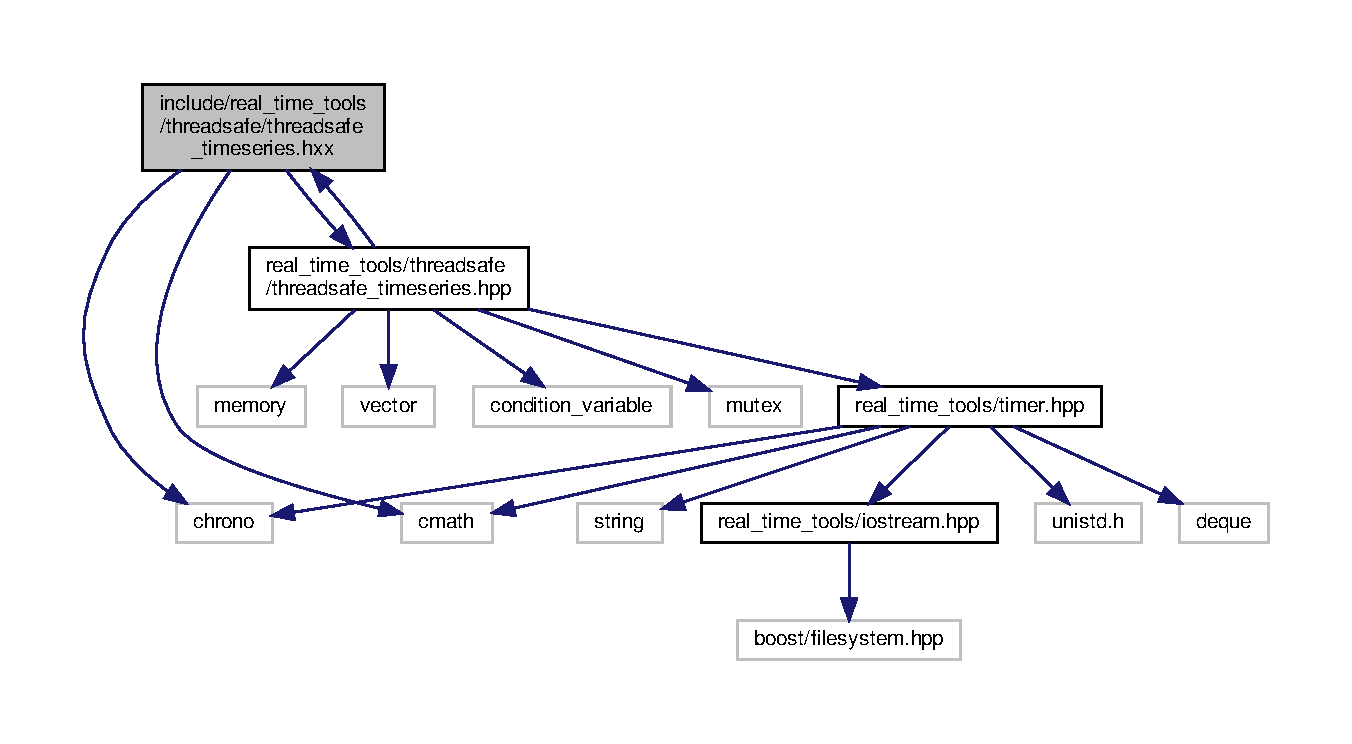
\includegraphics[width=350pt]{threadsafe__timeseries_8hxx__incl}
\end{center}
\end{figure}
This graph shows which files directly or indirectly include this file\+:
\nopagebreak
\begin{figure}[H]
\begin{center}
\leavevmode
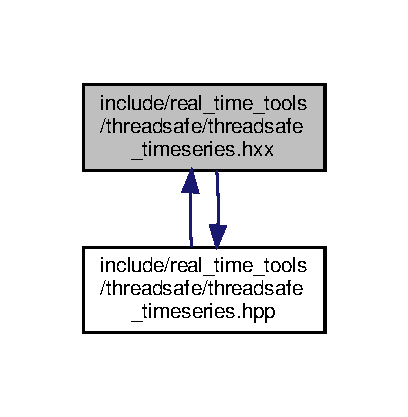
\includegraphics[width=196pt]{threadsafe__timeseries_8hxx__dep__incl}
\end{center}
\end{figure}


\subsection{Detailed Description}
This file contains the implementation of the class in \hyperlink{threadsafe__timeseries_8hpp}{threadsafe\+\_\+timeseries.\+hpp}. 

\begin{DoxyAuthor}{Author}
Manuel Wuthrich (\href{mailto:manuel.wuthrich@gmail.com}{\tt manuel.\+wuthrich@gmail.\+com}) 

Maximilien Naveau (\href{mailto:maximilien.naveau@gmail.com}{\tt maximilien.\+naveau@gmail.\+com}) 
\end{DoxyAuthor}
\begin{DoxyVersion}{Version}
0.\+1 
\end{DoxyVersion}
\begin{DoxyDate}{Date}
2018-\/11-\/27
\end{DoxyDate}
\begin{DoxyCopyright}{Copyright}
Copyright (c) 2018 
\end{DoxyCopyright}

\hypertarget{timer_8hpp}{}\section{include/real\+\_\+time\+\_\+tools/timer.hpp File Reference}
\label{timer_8hpp}\index{include/real\+\_\+time\+\_\+tools/timer.\+hpp@{include/real\+\_\+time\+\_\+tools/timer.\+hpp}}


Some tools to measure (ellapsed) time.  


{\ttfamily \#include $<$chrono$>$}\\*
{\ttfamily \#include $<$string$>$}\\*
{\ttfamily \#include $<$deque$>$}\\*
{\ttfamily \#include $<$cmath$>$}\\*
{\ttfamily \#include $<$unistd.\+h$>$}\\*
{\ttfamily \#include \char`\"{}real\+\_\+time\+\_\+tools/iostream.\+hpp\char`\"{}}\\*
Include dependency graph for timer.\+hpp\+:
\nopagebreak
\begin{figure}[H]
\begin{center}
\leavevmode
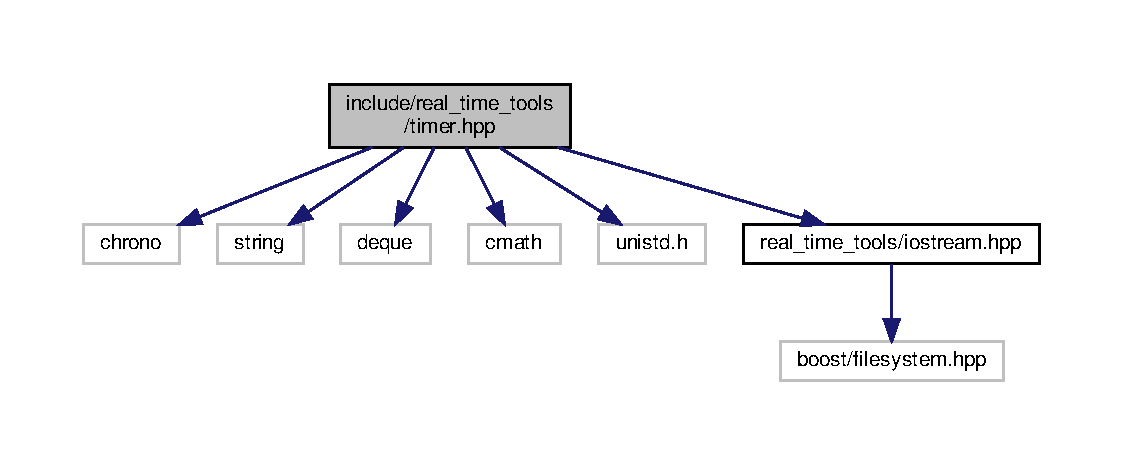
\includegraphics[width=350pt]{timer_8hpp__incl}
\end{center}
\end{figure}
This graph shows which files directly or indirectly include this file\+:
\nopagebreak
\begin{figure}[H]
\begin{center}
\leavevmode
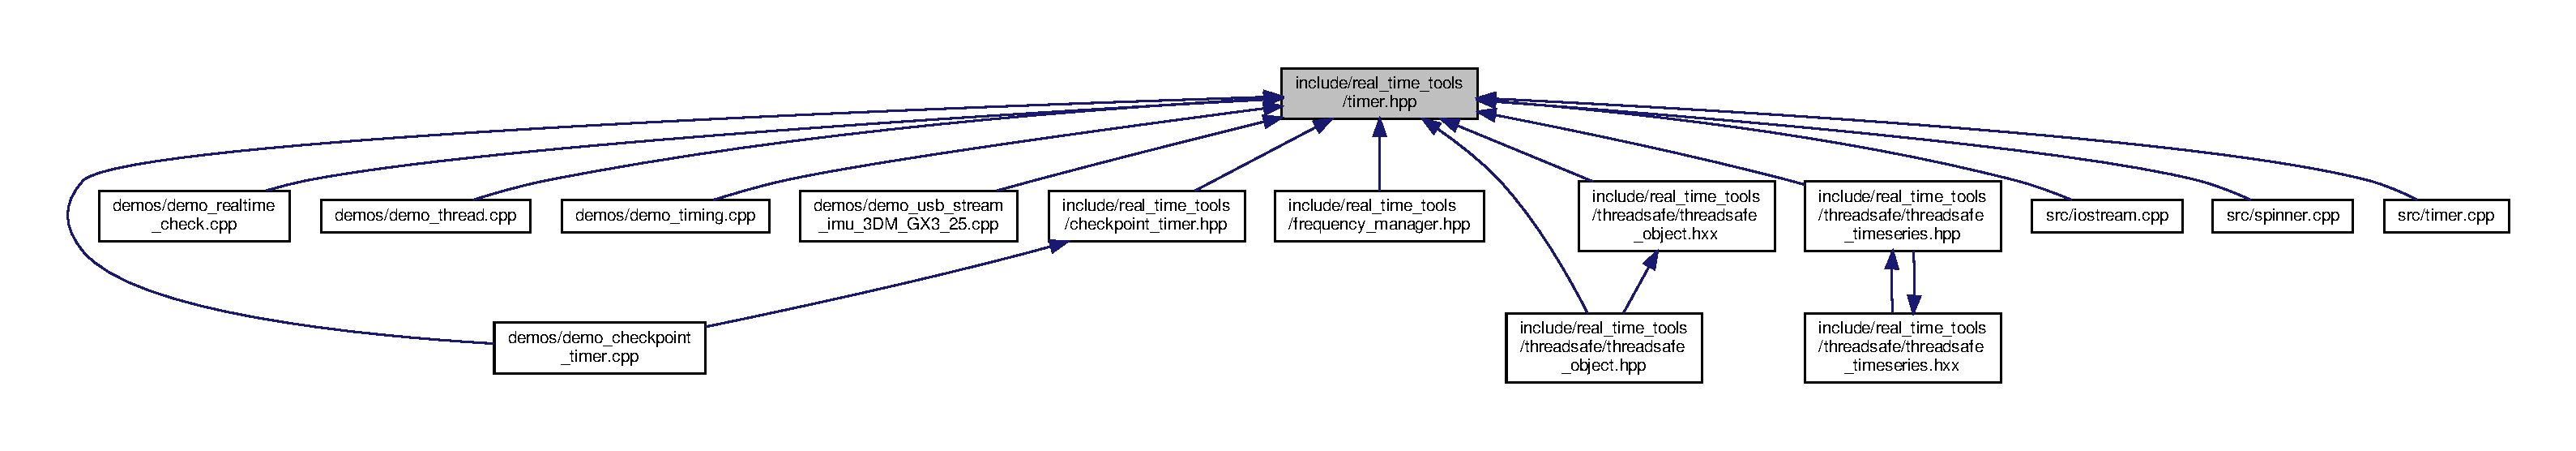
\includegraphics[width=350pt]{timer_8hpp__dep__incl}
\end{center}
\end{figure}
\subsection*{Classes}
\begin{DoxyCompactItemize}
\item 
class \hyperlink{classreal__time__tools_1_1Timer}{real\+\_\+time\+\_\+tools\+::\+Timer}
\begin{DoxyCompactList}\small\item\em The timer class is a simple time measurement class that measure between tic and tac and with a memory buffer of a certain size. \end{DoxyCompactList}\end{DoxyCompactItemize}


\subsection{Detailed Description}
Some tools to measure (ellapsed) time. 

\begin{DoxyAuthor}{Author}
Maximilien Naveau (\href{mailto:maximilien.naveau@gmail.com}{\tt maximilien.\+naveau@gmail.\+com}) license License B\+S\+D-\/3-\/\+Clause 
\end{DoxyAuthor}
\begin{DoxyCopyright}{Copyright}
Copyright (c) 2019, New York University and Max Planck Gesellschaft. 
\end{DoxyCopyright}
\begin{DoxyDate}{Date}
2019-\/05-\/22 
\end{DoxyDate}

\hypertarget{compute__statistics_8py}{}\section{src/bin/compute\+\_\+statistics.py File Reference}
\label{compute__statistics_8py}\index{src/bin/compute\+\_\+statistics.\+py@{src/bin/compute\+\_\+statistics.\+py}}


This program computes statistics from files in a user given folder. The files must possess at least 2 columns. The statistics are going to be computed from the econd one. The typical use is to give this executable a folder path and it will check all files with an extension ".dat" and perform the statistics.  


\subsection*{Functions}
\begin{DoxyCompactItemize}
\item 
def {\bfseries compute\+\_\+statistics.\+\_\+get\+\_\+all\+\_\+dat\+\_\+files} (folder)\hypertarget{compute__statistics_8py_a0489a5cc5b7c5e9b2bcf3ccfc75e9a74}{}\label{compute__statistics_8py_a0489a5cc5b7c5e9b2bcf3ccfc75e9a74}

\item 
def {\bfseries compute\+\_\+statistics.\+\_\+get\+\_\+data\+\_\+from\+\_\+file} (in\+\_\+file\+\_\+name)\hypertarget{compute__statistics_8py_a9839ab0f0089f8cb4807311df8a352cf}{}\label{compute__statistics_8py_a9839ab0f0089f8cb4807311df8a352cf}

\item 
def {\bfseries compute\+\_\+statistics.\+\_\+compute\+\_\+statitics} (data)\hypertarget{compute__statistics_8py_afe7eec3c0b928f482ac5cf67fc0d5660}{}\label{compute__statistics_8py_afe7eec3c0b928f482ac5cf67fc0d5660}

\item 
def {\bfseries compute\+\_\+statistics.\+main} (sys\+\_\+args)\hypertarget{compute__statistics_8py_a2fab7d549fda19c2b9123657f8fe90cf}{}\label{compute__statistics_8py_a2fab7d549fda19c2b9123657f8fe90cf}

\end{DoxyCompactItemize}


\subsection{Detailed Description}
This program computes statistics from files in a user given folder. The files must possess at least 2 columns. The statistics are going to be computed from the econd one. The typical use is to give this executable a folder path and it will check all files with an extension ".dat" and perform the statistics. 

\begin{DoxyAuthor}{Author}
Maximilien Naveau (\href{mailto:maximilien.naveau@gmail.com}{\tt maximilien.\+naveau@gmail.\+com}) 
\end{DoxyAuthor}
\begin{DoxyCopyright}{Copyright}
Copyright (c) 2019, New York University and Max Planck Gesellschaft. 
\end{DoxyCopyright}
\begin{DoxyRefDesc}{License}
\item[\hyperlink{license__license000005}{License}]License B\+S\+D-\/3 clause \end{DoxyRefDesc}
\begin{DoxyDate}{Date}
2019-\/05-\/06 
\end{DoxyDate}

\hypertarget{realtime__test_8cpp}{}\section{src/bin/realtime\+\_\+test.cpp File Reference}
\label{realtime__test_8cpp}\index{src/bin/realtime\+\_\+test.\+cpp@{src/bin/realtime\+\_\+test.\+cpp}}


Program\+: test the real time capabilities of a machine.  


{\ttfamily \#include \char`\"{}real\+\_\+time\+\_\+tools/realtime\+\_\+test.\+hpp\char`\"{}}\newline
{\ttfamily \#include $<$signal.\+h$>$}\newline
{\ttfamily \#include $<$atomic$>$}\newline
{\ttfamily \#include $<$memory$>$}\newline
{\ttfamily \#include \char`\"{}real\+\_\+time\+\_\+tools/realtime\+\_\+check.\+hpp\char`\"{}}\newline
{\ttfamily \#include \char`\"{}real\+\_\+time\+\_\+tools/spinner.\+hpp\char`\"{}}\newline
{\ttfamily \#include \char`\"{}real\+\_\+time\+\_\+tools/thread.\+hpp\char`\"{}}\newline
{\ttfamily \#include \char`\"{}shared\+\_\+memory/shared\+\_\+memory.\+hpp\char`\"{}}\newline
Include dependency graph for realtime\+\_\+test.\+cpp\+:
\nopagebreak
\begin{figure}[H]
\begin{center}
\leavevmode
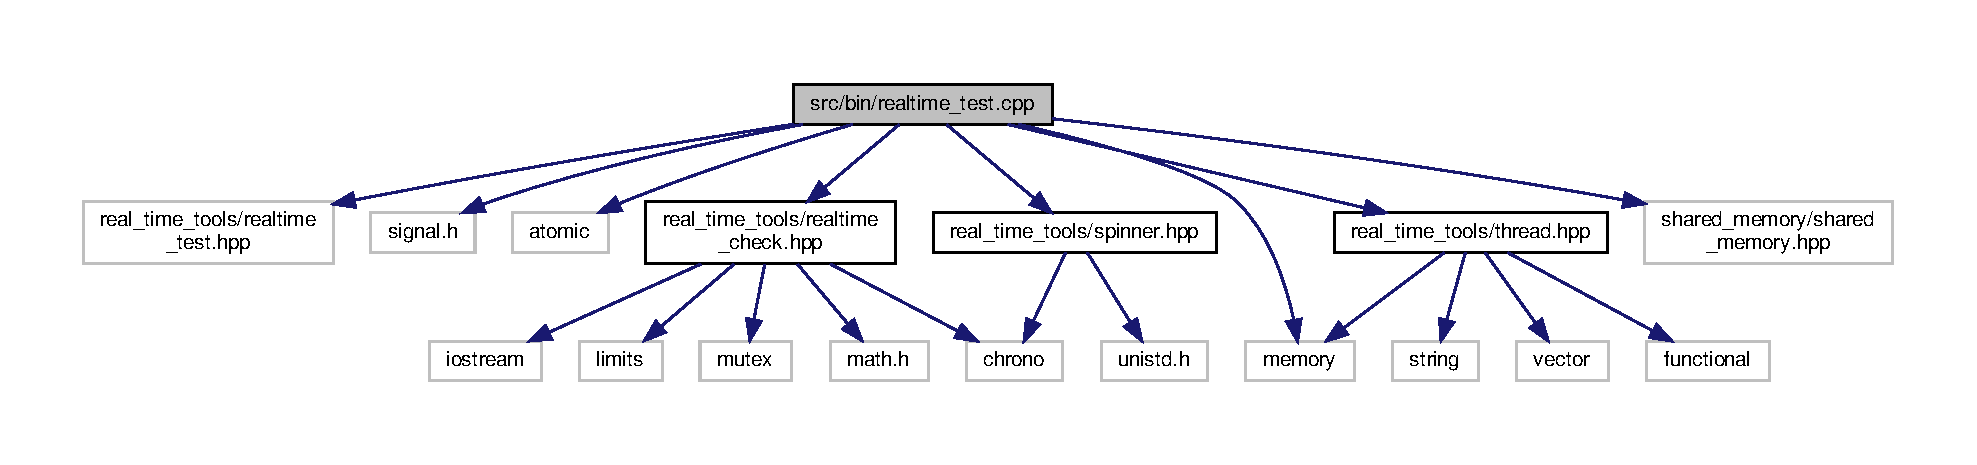
\includegraphics[width=350pt]{realtime__test_8cpp__incl}
\end{center}
\end{figure}
\subsection*{Classes}
\begin{DoxyCompactItemize}
\item 
class \hyperlink{classConfiguration}{Configuration}
\begin{DoxyCompactList}\small\item\em \hyperlink{classConfiguration}{Configuration} of the test thread. \end{DoxyCompactList}\item 
class \hyperlink{classComputation}{Computation}
\begin{DoxyCompactList}\small\item\em Abstract interface for some different thread computation. \end{DoxyCompactList}\item 
class \hyperlink{classMatrix__computation__no__eigen}{Matrix\+\_\+computation\+\_\+no\+\_\+eigen}
\begin{DoxyCompactList}\small\item\em Some specific computation based on matrix multiplication. \end{DoxyCompactList}\end{DoxyCompactItemize}
\subsection*{Functions}
\begin{DoxyCompactItemize}
\item 
\mbox{\Hypertarget{realtime__test_8cpp_a54b1343eb90254009bd964c44996761b}\label{realtime__test_8cpp_a54b1343eb90254009bd964c44996761b}} 
void $\ast$ \hyperlink{realtime__test_8cpp_a54b1343eb90254009bd964c44996761b}{thread\+\_\+function} (void $\ast$v)
\begin{DoxyCompactList}\small\item\em This is the real time thread that perform the check and the computations. \end{DoxyCompactList}\item 
void \hyperlink{realtime__test_8cpp_ae5ad5cbeccaedc03a48d3c7eaa803e79}{print\+\_\+usage} ()
\begin{DoxyCompactList}\small\item\em Display the usage in case of a miss-\/use. \end{DoxyCompactList}\item 
\mbox{\Hypertarget{realtime__test_8cpp_acbd189ad2c6253bfe6cd5a3a2e20d117}\label{realtime__test_8cpp_acbd189ad2c6253bfe6cd5a3a2e20d117}} 
bool \hyperlink{realtime__test_8cpp_acbd189ad2c6253bfe6cd5a3a2e20d117}{set\+\_\+config} (int nb\+\_\+args, char $\ast$$\ast$args, \hyperlink{classConfiguration}{Configuration} \&config)
\begin{DoxyCompactList}\small\item\em parse the input argument and configure which conputation should be done \end{DoxyCompactList}\item 
\mbox{\Hypertarget{realtime__test_8cpp_ae7878b49a48dc0ca3bcb00390121cf5f}\label{realtime__test_8cpp_ae7878b49a48dc0ca3bcb00390121cf5f}} 
void \hyperlink{realtime__test_8cpp_ae7878b49a48dc0ca3bcb00390121cf5f}{clean\+\_\+memory} ()
\begin{DoxyCompactList}\small\item\em Delete the shared memeory. \end{DoxyCompactList}\item 
void \hyperlink{realtime__test_8cpp_aba399b0a6a6e3bd37af95bd04e8def6f}{stop} (int)
\begin{DoxyCompactList}\small\item\em stop the current thread. \end{DoxyCompactList}\item 
int \hyperlink{realtime__test_8cpp_af4978f2751bdb780c0a97d67d65dd405}{main} (int nb\+\_\+args, char $\ast$$\ast$argv)
\begin{DoxyCompactList}\small\item\em This program evaulate the quality of the frequency tracking by a real time thread. \end{DoxyCompactList}\end{DoxyCompactItemize}
\subsection*{Variables}
\begin{DoxyCompactItemize}
\item 
\mbox{\Hypertarget{realtime__test_8cpp_aa25458bfbc45f5dca35aa414759acafd}\label{realtime__test_8cpp_aa25458bfbc45f5dca35aa414759acafd}} 
static int \hyperlink{realtime__test_8cpp_aa25458bfbc45f5dca35aa414759acafd}{M\+A\+T\+R\+I\+X\+\_\+\+C\+O\+M\+P\+U\+T\+A\+T\+I\+O\+N\+\_\+\+N\+O\+\_\+\+E\+I\+G\+E\+N\+\_\+64} = 1
\begin{DoxyCompactList}\small\item\em valid modes, creating subclasses of \hyperlink{classComputation}{Computation} to add new ones (see below) \end{DoxyCompactList}\item 
\mbox{\Hypertarget{realtime__test_8cpp_a5a5fc9f109f74c744e4e8739c6cae510}\label{realtime__test_8cpp_a5a5fc9f109f74c744e4e8739c6cae510}} 
std\+::atomic$<$ bool $>$ \hyperlink{realtime__test_8cpp_a5a5fc9f109f74c744e4e8739c6cae510}{R\+U\+N\+N\+I\+NG}
\begin{DoxyCompactList}\small\item\em Is the thread running? \end{DoxyCompactList}\end{DoxyCompactItemize}


\subsection{Detailed Description}
Program\+: test the real time capabilities of a machine. 

\begin{DoxyAuthor}{Author}
Maximilien Naveau (\href{mailto:maximilien.naveau@gmail.com}{\tt maximilien.\+naveau@gmail.\+com}) license License B\+S\+D-\/3-\/\+Clause 
\end{DoxyAuthor}
\begin{DoxyCopyright}{Copyright}
Copyright (c) 2019, New York University and Max Planck Gesellschaft. 
\end{DoxyCopyright}
\begin{DoxyDate}{Date}
2019-\/05-\/22 
\end{DoxyDate}


\subsection{Function Documentation}
\mbox{\Hypertarget{realtime__test_8cpp_af4978f2751bdb780c0a97d67d65dd405}\label{realtime__test_8cpp_af4978f2751bdb780c0a97d67d65dd405}} 
\index{realtime\+\_\+test.\+cpp@{realtime\+\_\+test.\+cpp}!main@{main}}
\index{main@{main}!realtime\+\_\+test.\+cpp@{realtime\+\_\+test.\+cpp}}
\subsubsection{\texorpdfstring{main()}{main()}}
{\footnotesize\ttfamily int main (\begin{DoxyParamCaption}\item[{int}]{nb\+\_\+args,  }\item[{char $\ast$$\ast$}]{argv }\end{DoxyParamCaption})}



This program evaulate the quality of the frequency tracking by a real time thread. 

\mbox{\Hypertarget{realtime__test_8cpp_ae5ad5cbeccaedc03a48d3c7eaa803e79}\label{realtime__test_8cpp_ae5ad5cbeccaedc03a48d3c7eaa803e79}} 
\index{realtime\+\_\+test.\+cpp@{realtime\+\_\+test.\+cpp}!print\+\_\+usage@{print\+\_\+usage}}
\index{print\+\_\+usage@{print\+\_\+usage}!realtime\+\_\+test.\+cpp@{realtime\+\_\+test.\+cpp}}
\subsubsection{\texorpdfstring{print\+\_\+usage()}{print\_usage()}}
{\footnotesize\ttfamily void print\+\_\+usage (\begin{DoxyParamCaption}{ }\end{DoxyParamCaption})}



Display the usage in case of a miss-\/use. 

\mbox{\Hypertarget{realtime__test_8cpp_aba399b0a6a6e3bd37af95bd04e8def6f}\label{realtime__test_8cpp_aba399b0a6a6e3bd37af95bd04e8def6f}} 
\index{realtime\+\_\+test.\+cpp@{realtime\+\_\+test.\+cpp}!stop@{stop}}
\index{stop@{stop}!realtime\+\_\+test.\+cpp@{realtime\+\_\+test.\+cpp}}
\subsubsection{\texorpdfstring{stop()}{stop()}}
{\footnotesize\ttfamily void stop (\begin{DoxyParamCaption}\item[{int}]{ }\end{DoxyParamCaption})}



stop the current thread. 

This method is called throw a \char`\"{}ctrl+c\char`\"{} \begin{Desc}
\item[Examples\+: ]\par
\hyperlink{demo_realtime_strict_check_8cpp-example}{demo\+\_\+realtime\+\_\+strict\+\_\+check.\+cpp}.\end{Desc}

\hypertarget{realtime__test__display_8cpp}{}\section{src/bin/realtime\+\_\+test\+\_\+display.cpp File Reference}
\label{realtime__test__display_8cpp}\index{src/bin/realtime\+\_\+test\+\_\+display.\+cpp@{src/bin/realtime\+\_\+test\+\_\+display.\+cpp}}


Display results of the real time test.  


{\ttfamily \#include $<$signal.\+h$>$}\newline
{\ttfamily \#include \char`\"{}real\+\_\+time\+\_\+tools/realtime\+\_\+test.\+hpp\char`\"{}}\newline
{\ttfamily \#include \char`\"{}real\+\_\+time\+\_\+tools/spinner.\+hpp\char`\"{}}\newline
{\ttfamily \#include \char`\"{}shared\+\_\+memory/shared\+\_\+memory.\+hpp\char`\"{}}\newline
Include dependency graph for realtime\+\_\+test\+\_\+display.\+cpp\+:
\nopagebreak
\begin{figure}[H]
\begin{center}
\leavevmode
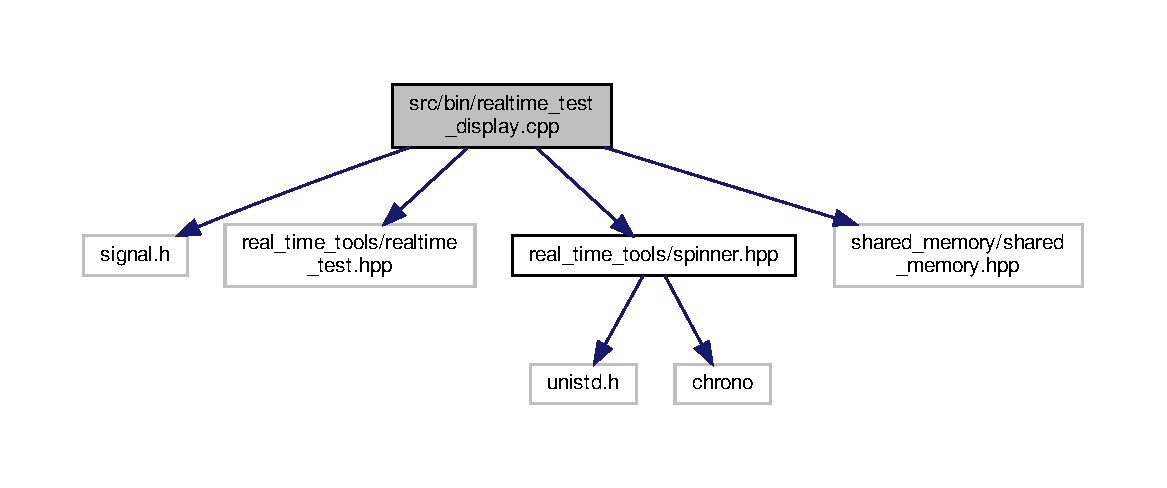
\includegraphics[width=350pt]{realtime__test__display_8cpp__incl}
\end{center}
\end{figure}
\subsection*{Functions}
\begin{DoxyCompactItemize}
\item 
void \hyperlink{realtime__test__display_8cpp_aba399b0a6a6e3bd37af95bd04e8def6f}{stop} (int)
\begin{DoxyCompactList}\small\item\em Method run upon ctrl+c. \end{DoxyCompactList}\item 
int \hyperlink{realtime__test__display_8cpp_a2c3f6775325c30275d11c6abee2db6a0}{main} (int, char $\ast$$\ast$)
\begin{DoxyCompactList}\small\item\em This program analyze the data computed by the real\+\_\+time\+\_\+test executable. \end{DoxyCompactList}\end{DoxyCompactItemize}
\subsection*{Variables}
\begin{DoxyCompactItemize}
\item 
static bool \hyperlink{realtime__test__display_8cpp_a36f7b6be7108281af77939ceaec42fd6}{running}
\begin{DoxyCompactList}\small\item\em Global boolean to manage the thread loop stop on ctrl+c. \end{DoxyCompactList}\end{DoxyCompactItemize}


\subsection{Detailed Description}
Display results of the real time test. 

\begin{DoxyAuthor}{Author}
Maximilien Naveau (\href{mailto:maximilien.naveau@gmail.com}{\tt maximilien.\+naveau@gmail.\+com}) license License B\+S\+D-\/3-\/\+Clause 
\end{DoxyAuthor}
\begin{DoxyCopyright}{Copyright}
Copyright (c) 2019, New York University and Max Planck Gesellschaft. 
\end{DoxyCopyright}
\begin{DoxyDate}{Date}
2019-\/05-\/22 
\end{DoxyDate}


\subsection{Function Documentation}
\mbox{\Hypertarget{realtime__test__display_8cpp_a2c3f6775325c30275d11c6abee2db6a0}\label{realtime__test__display_8cpp_a2c3f6775325c30275d11c6abee2db6a0}} 
\index{realtime\+\_\+test\+\_\+display.\+cpp@{realtime\+\_\+test\+\_\+display.\+cpp}!main@{main}}
\index{main@{main}!realtime\+\_\+test\+\_\+display.\+cpp@{realtime\+\_\+test\+\_\+display.\+cpp}}
\subsubsection{\texorpdfstring{main()}{main()}}
{\footnotesize\ttfamily int main (\begin{DoxyParamCaption}\item[{int}]{,  }\item[{char $\ast$$\ast$}]{ }\end{DoxyParamCaption})}



This program analyze the data computed by the real\+\_\+time\+\_\+test executable. 

Both processes communicate throw a shared memeory.

\begin{DoxyReturn}{Returns}
int 0 
\end{DoxyReturn}
\mbox{\Hypertarget{realtime__test__display_8cpp_aba399b0a6a6e3bd37af95bd04e8def6f}\label{realtime__test__display_8cpp_aba399b0a6a6e3bd37af95bd04e8def6f}} 
\index{realtime\+\_\+test\+\_\+display.\+cpp@{realtime\+\_\+test\+\_\+display.\+cpp}!stop@{stop}}
\index{stop@{stop}!realtime\+\_\+test\+\_\+display.\+cpp@{realtime\+\_\+test\+\_\+display.\+cpp}}
\subsubsection{\texorpdfstring{stop()}{stop()}}
{\footnotesize\ttfamily void stop (\begin{DoxyParamCaption}\item[{int}]{ }\end{DoxyParamCaption})}



Method run upon ctrl+c. 

Stops the loop. 

\subsection{Variable Documentation}
\mbox{\Hypertarget{realtime__test__display_8cpp_a36f7b6be7108281af77939ceaec42fd6}\label{realtime__test__display_8cpp_a36f7b6be7108281af77939ceaec42fd6}} 
\index{realtime\+\_\+test\+\_\+display.\+cpp@{realtime\+\_\+test\+\_\+display.\+cpp}!running@{running}}
\index{running@{running}!realtime\+\_\+test\+\_\+display.\+cpp@{realtime\+\_\+test\+\_\+display.\+cpp}}
\subsubsection{\texorpdfstring{running}{running}}
{\footnotesize\ttfamily bool running\hspace{0.3cm}{\ttfamily [static]}}



Global boolean to manage the thread loop stop on ctrl+c. 


\hypertarget{iostream_8cpp}{}\section{src/iostream.cpp File Reference}
\label{iostream_8cpp}\index{src/iostream.\+cpp@{src/iostream.\+cpp}}


implement some cross platform utilities to create folder or detect the home folder, etc.  


{\ttfamily \#include $<$sstream$>$}\\*
{\ttfamily \#include \char`\"{}real\+\_\+time\+\_\+tools/timer.\+hpp\char`\"{}}\\*
{\ttfamily \#include \char`\"{}real\+\_\+time\+\_\+tools/iostream.\+hpp\char`\"{}}\\*
Include dependency graph for iostream.\+cpp\+:
\nopagebreak
\begin{figure}[H]
\begin{center}
\leavevmode
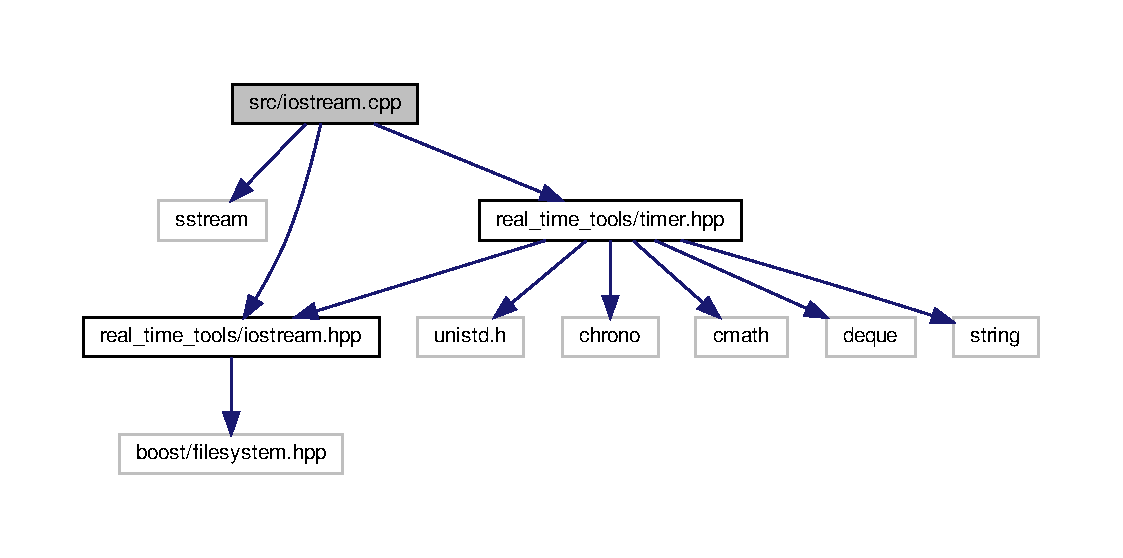
\includegraphics[width=350pt]{iostream_8cpp__incl}
\end{center}
\end{figure}
\subsection*{Functions}
\begin{DoxyCompactItemize}
\item 
std\+::string \hyperlink{iostream_8hpp_a5146f16f97588edcc7dbe28641f4a1fd}{real\+\_\+time\+\_\+tools\+::get\+\_\+log\+\_\+dir} (std\+::string app\+\_\+name)
\begin{DoxyCompactList}\small\item\em Get the logging directory based on a specific application. \end{DoxyCompactList}\item 
bool \hyperlink{iostream_8hpp_a4ce01145e1d43fc6f54c3f654de5bd7d}{real\+\_\+time\+\_\+tools\+::create\+\_\+directory} (std\+::string path)
\begin{DoxyCompactList}\small\item\em Create a directory. \end{DoxyCompactList}\item 
std\+::string \hyperlink{iostream_8hpp_a21f87296dd11ab3784e7b793033a21ed}{real\+\_\+time\+\_\+tools\+::get\+\_\+home\+\_\+dir} ()
\begin{DoxyCompactList}\small\item\em Get the home directory path. \end{DoxyCompactList}\end{DoxyCompactItemize}


\subsection{Detailed Description}
implement some cross platform utilities to create folder or detect the home folder, etc. 

\begin{DoxyAuthor}{Author}
Maximilien Naveau (\href{mailto:maximilien.naveau@gmail.com}{\tt maximilien.\+naveau@gmail.\+com}) license License B\+S\+D-\/3-\/\+Clause 
\end{DoxyAuthor}
\begin{DoxyCopyright}{Copyright}
Copyright (c) 2019, New York University and Max Planck Gesellschaft. 
\end{DoxyCopyright}
\begin{DoxyDate}{Date}
2019-\/05-\/22 
\end{DoxyDate}


\subsection{Function Documentation}
\index{iostream.\+cpp@{iostream.\+cpp}!create\+\_\+directory@{create\+\_\+directory}}
\index{create\+\_\+directory@{create\+\_\+directory}!iostream.\+cpp@{iostream.\+cpp}}
\subsubsection[{\texorpdfstring{create\+\_\+directory(std\+::string path)}{create_directory(std::string path)}}]{\setlength{\rightskip}{0pt plus 5cm}bool real\+\_\+time\+\_\+tools\+::create\+\_\+directory (
\begin{DoxyParamCaption}
\item[{std\+::string}]{path}
\end{DoxyParamCaption}
)}\hypertarget{iostream_8hpp_file_a4ce01145e1d43fc6f54c3f654de5bd7d}{}\label{iostream_8hpp_file_a4ce01145e1d43fc6f54c3f654de5bd7d}


Create a directory. 


\begin{DoxyParams}{Parameters}
{\em path} & is the path to be created \\
\hline
\end{DoxyParams}
\begin{DoxyReturn}{Returns}
true if everything went well 

false if a problem occur 
\end{DoxyReturn}
\index{iostream.\+cpp@{iostream.\+cpp}!get\+\_\+home\+\_\+dir@{get\+\_\+home\+\_\+dir}}
\index{get\+\_\+home\+\_\+dir@{get\+\_\+home\+\_\+dir}!iostream.\+cpp@{iostream.\+cpp}}
\subsubsection[{\texorpdfstring{get\+\_\+home\+\_\+dir()}{get_home_dir()}}]{\setlength{\rightskip}{0pt plus 5cm}std\+::string real\+\_\+time\+\_\+tools\+::get\+\_\+home\+\_\+dir (
\begin{DoxyParamCaption}
{}
\end{DoxyParamCaption}
)}\hypertarget{iostream_8hpp_file_a21f87296dd11ab3784e7b793033a21ed}{}\label{iostream_8hpp_file_a21f87296dd11ab3784e7b793033a21ed}


Get the home directory path. 

\begin{DoxyReturn}{Returns}
std\+::string the home directory absolute path ending with a \char`\"{}/\char`\"{} 
\end{DoxyReturn}
\index{iostream.\+cpp@{iostream.\+cpp}!get\+\_\+log\+\_\+dir@{get\+\_\+log\+\_\+dir}}
\index{get\+\_\+log\+\_\+dir@{get\+\_\+log\+\_\+dir}!iostream.\+cpp@{iostream.\+cpp}}
\subsubsection[{\texorpdfstring{get\+\_\+log\+\_\+dir(std\+::string app\+\_\+name)}{get_log_dir(std::string app_name)}}]{\setlength{\rightskip}{0pt plus 5cm}std\+::string real\+\_\+time\+\_\+tools\+::get\+\_\+log\+\_\+dir (
\begin{DoxyParamCaption}
\item[{std\+::string}]{app\+\_\+name}
\end{DoxyParamCaption}
)}\hypertarget{iostream_8hpp_file_a5146f16f97588edcc7dbe28641f4a1fd}{}\label{iostream_8hpp_file_a5146f16f97588edcc7dbe28641f4a1fd}


Get the logging directory based on a specific application. 

It creates a direction in \$\+H\+O\+ME/app\+\_\+name/\+Y\+E\+A\+R\+\_\+\+M\+O\+N\+T\+H\+\_\+\+D\+A\+Y\+\_\+\+H\+O\+U\+R\+\_\+\+S\+E\+C\+O\+N\+D/ and return the absolute path of this. It allows the user to dump data in different folders everytime the user launch the application.


\begin{DoxyParams}{Parameters}
{\em app\+\_\+name} & is the application name \\
\hline
\end{DoxyParams}
\begin{DoxyReturn}{Returns}
std\+::string the absolute path to the log directory 
\end{DoxyReturn}

\hypertarget{process__manager_8cpp}{}\section{src/process\+\_\+manager.cpp File Reference}
\label{process__manager_8cpp}\index{src/process\+\_\+manager.\+cpp@{src/process\+\_\+manager.\+cpp}}


Allow us to fix the current process to a specific set of cpus.  


{\ttfamily \#include $<$stdio.\+h$>$}\\*
{\ttfamily \#include $<$sys/types.\+h$>$}\\*
{\ttfamily \#include $<$sys/stat.\+h$>$}\\*
{\ttfamily \#include $<$fcntl.\+h$>$}\\*
{\ttfamily \#include $<$stdint.\+h$>$}\\*
{\ttfamily \#include $<$stdlib.\+h$>$}\\*
{\ttfamily \#include $<$unistd.\+h$>$}\\*
{\ttfamily \#include $<$vector$>$}\\*
{\ttfamily \#include \char`\"{}real\+\_\+time\+\_\+tools/iostream.\+hpp\char`\"{}}\\*
{\ttfamily \#include \char`\"{}real\+\_\+time\+\_\+tools/process\+\_\+manager.\+hpp\char`\"{}}\\*
Include dependency graph for process\+\_\+manager.\+cpp\+:
\nopagebreak
\begin{figure}[H]
\begin{center}
\leavevmode
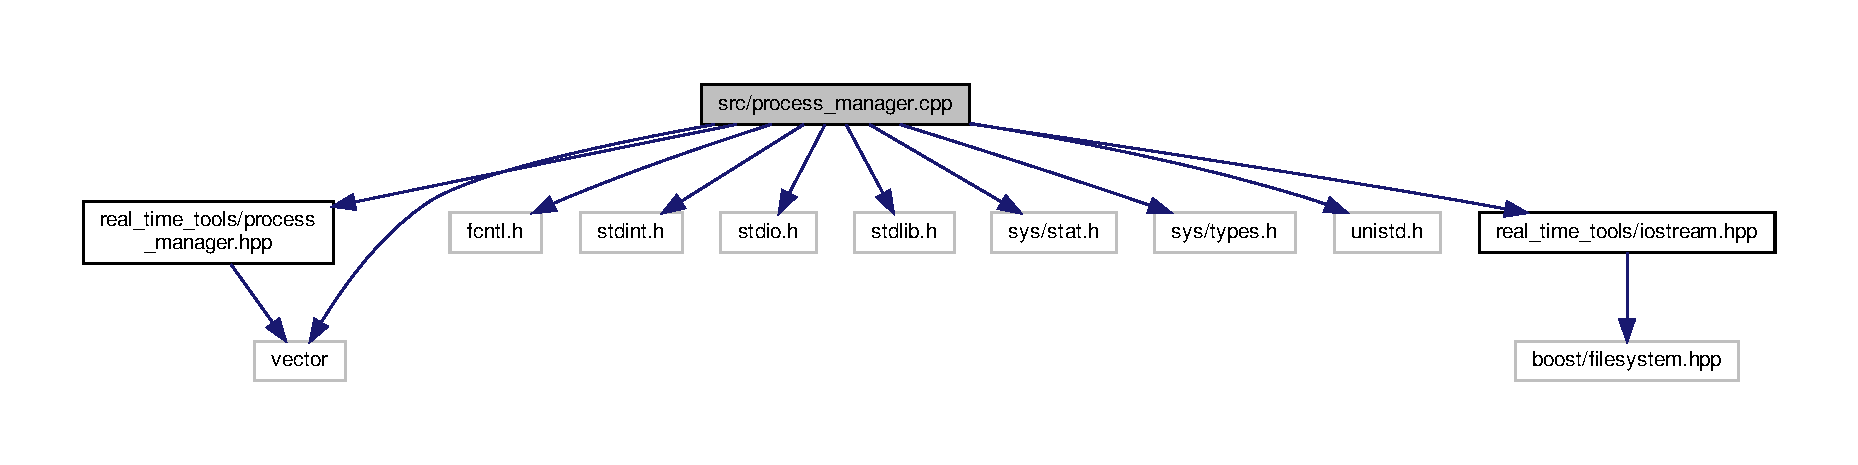
\includegraphics[width=350pt]{process__manager_8cpp__incl}
\end{center}
\end{figure}
\subsection*{Functions}
\begin{DoxyCompactItemize}
\item 
bool \hyperlink{process__manager_8hpp_ae4959078e00ed85dd26b9a96dcd8fd3b}{real\+\_\+time\+\_\+tools\+::fix\+\_\+current\+\_\+process\+\_\+to\+\_\+cpu} (std\+::vector$<$ int $>$ \&cpu\+\_\+affinities, int pid)
\begin{DoxyCompactList}\small\item\em Pin an executing process to a specific C\+PU in order to avoid jumps between C\+P\+Us. \end{DoxyCompactList}\item 
bool \hyperlink{process__manager_8hpp_a6a8ceffef6761ee22e436a1151f020af}{real\+\_\+time\+\_\+tools\+::set\+\_\+cpu\+\_\+dma\+\_\+latency} (int max\+\_\+latency\+\_\+us)
\begin{DoxyCompactList}\small\item\em Set the \+\_\+cpu\+\_\+dma\+\_\+latency object\+We can set the maximum C\+PU latency for processes in micro seconds. \end{DoxyCompactList}\end{DoxyCompactItemize}


\subsection{Detailed Description}
Allow us to fix the current process to a specific set of cpus. 

\begin{DoxyAuthor}{Author}
Maximilien Naveau (\href{mailto:maximilien.naveau@gmail.com}{\tt maximilien.\+naveau@gmail.\+com}) license License B\+S\+D-\/3-\/\+Clause 
\end{DoxyAuthor}
\begin{DoxyCopyright}{Copyright}
Copyright (c) 2019, New York University and Max Planck Gesellschaft. 
\end{DoxyCopyright}
\begin{DoxyDate}{Date}
2019-\/05-\/22 
\end{DoxyDate}


\subsection{Function Documentation}
\index{process\+\_\+manager.\+cpp@{process\+\_\+manager.\+cpp}!fix\+\_\+current\+\_\+process\+\_\+to\+\_\+cpu@{fix\+\_\+current\+\_\+process\+\_\+to\+\_\+cpu}}
\index{fix\+\_\+current\+\_\+process\+\_\+to\+\_\+cpu@{fix\+\_\+current\+\_\+process\+\_\+to\+\_\+cpu}!process\+\_\+manager.\+cpp@{process\+\_\+manager.\+cpp}}
\subsubsection[{\texorpdfstring{fix\+\_\+current\+\_\+process\+\_\+to\+\_\+cpu(std\+::vector$<$ int $>$ \&cpu\+\_\+affinities, int pid)}{fix_current_process_to_cpu(std::vector< int > &cpu_affinities, int pid)}}]{\setlength{\rightskip}{0pt plus 5cm}bool real\+\_\+time\+\_\+tools\+::fix\+\_\+current\+\_\+process\+\_\+to\+\_\+cpu (
\begin{DoxyParamCaption}
\item[{std\+::vector$<$ int $>$ \&}]{cpu\+\_\+affinities, }
\item[{int}]{pid}
\end{DoxyParamCaption}
)}\hypertarget{process__manager_8hpp_file_ae4959078e00ed85dd26b9a96dcd8fd3b}{}\label{process__manager_8hpp_file_ae4959078e00ed85dd26b9a96dcd8fd3b}


Pin an executing process to a specific C\+PU in order to avoid jumps between C\+P\+Us. 


\begin{DoxyParams}{Parameters}
{\em cpu\+\_\+affinities} & is the index of the C\+PU one wants to pin the process on. \\
\hline
{\em pid} & is the P\+ID of the current process. \\
\hline
\end{DoxyParams}
\begin{DoxyReturn}{Returns}
true if everything went well. 

false otherwise 
\end{DoxyReturn}
\index{process\+\_\+manager.\+cpp@{process\+\_\+manager.\+cpp}!set\+\_\+cpu\+\_\+dma\+\_\+latency@{set\+\_\+cpu\+\_\+dma\+\_\+latency}}
\index{set\+\_\+cpu\+\_\+dma\+\_\+latency@{set\+\_\+cpu\+\_\+dma\+\_\+latency}!process\+\_\+manager.\+cpp@{process\+\_\+manager.\+cpp}}
\subsubsection[{\texorpdfstring{set\+\_\+cpu\+\_\+dma\+\_\+latency(int max\+\_\+latency\+\_\+us)}{set_cpu_dma_latency(int max_latency_us)}}]{\setlength{\rightskip}{0pt plus 5cm}bool real\+\_\+time\+\_\+tools\+::set\+\_\+cpu\+\_\+dma\+\_\+latency (
\begin{DoxyParamCaption}
\item[{int}]{max\+\_\+latency\+\_\+us}
\end{DoxyParamCaption}
)}\hypertarget{process__manager_8hpp_file_a6a8ceffef6761ee22e436a1151f020af}{}\label{process__manager_8hpp_file_a6a8ceffef6761ee22e436a1151f020af}


Set the \+\_\+cpu\+\_\+dma\+\_\+latency object\+We can set the maximum C\+PU latency for processes in micro seconds. 


\begin{DoxyParams}{Parameters}
{\em max\+\_\+latency\+\_\+us} & is the maximum latency in micro-\/seconds. \\
\hline
\end{DoxyParams}
\begin{DoxyReturn}{Returns}
true if everything went well. 

false if something went wrong. 
\end{DoxyReturn}

\hypertarget{realtime__check_8cpp}{}\section{src/realtime\+\_\+check.cpp File Reference}
\label{realtime__check_8cpp}\index{src/realtime\+\_\+check.\+cpp@{src/realtime\+\_\+check.\+cpp}}


Utilities to check if the real\+\_\+time capabilities of an algorithm is maintained or not.  


{\ttfamily \#include \char`\"{}real\+\_\+time\+\_\+tools/realtime\+\_\+check.\+hpp\char`\"{}}\\*
{\ttfamily \#include $<$fstream$>$}\\*
Include dependency graph for realtime\+\_\+check.\+cpp\+:
\nopagebreak
\begin{figure}[H]
\begin{center}
\leavevmode
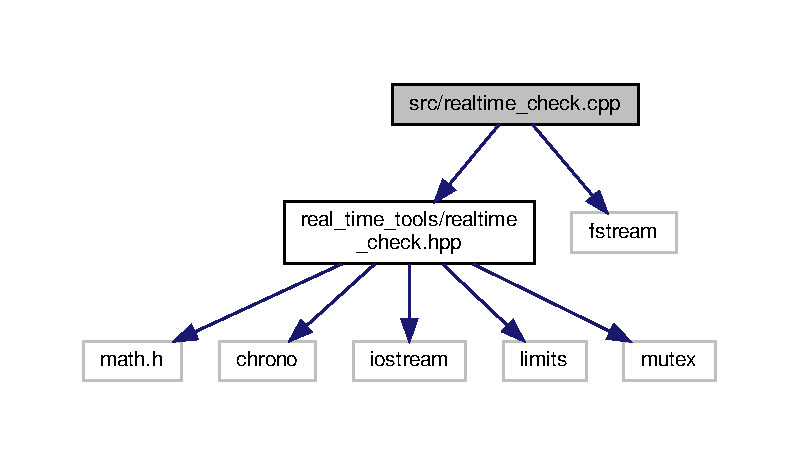
\includegraphics[width=350pt]{realtime__check_8cpp__incl}
\end{center}
\end{figure}


\subsection{Detailed Description}
Utilities to check if the real\+\_\+time capabilities of an algorithm is maintained or not. 

\begin{DoxyAuthor}{Author}
Maximilien Naveau (\href{mailto:maximilien.naveau@gmail.com}{\tt maximilien.\+naveau@gmail.\+com}) license License B\+S\+D-\/3-\/\+Clause 
\end{DoxyAuthor}
\begin{DoxyCopyright}{Copyright}
Copyright (c) 2019, New York University and Max Planck Gesellschaft. 
\end{DoxyCopyright}
\begin{DoxyDate}{Date}
2019-\/05-\/22 
\end{DoxyDate}

\hypertarget{spinner_8cpp}{}\section{src/spinner.cpp File Reference}
\label{spinner_8cpp}\index{src/spinner.\+cpp@{src/spinner.\+cpp}}


This file implements a spinner to time a loop.  


{\ttfamily \#include $<$real\+\_\+time\+\_\+tools/timer.\+hpp$>$}\\*
{\ttfamily \#include $<$real\+\_\+time\+\_\+tools/spinner.\+hpp$>$}\\*
{\ttfamily \#include $<$iostream$>$}\\*
{\ttfamily \#include $<$pthread.\+h$>$}\\*
Include dependency graph for spinner.\+cpp\+:
\nopagebreak
\begin{figure}[H]
\begin{center}
\leavevmode
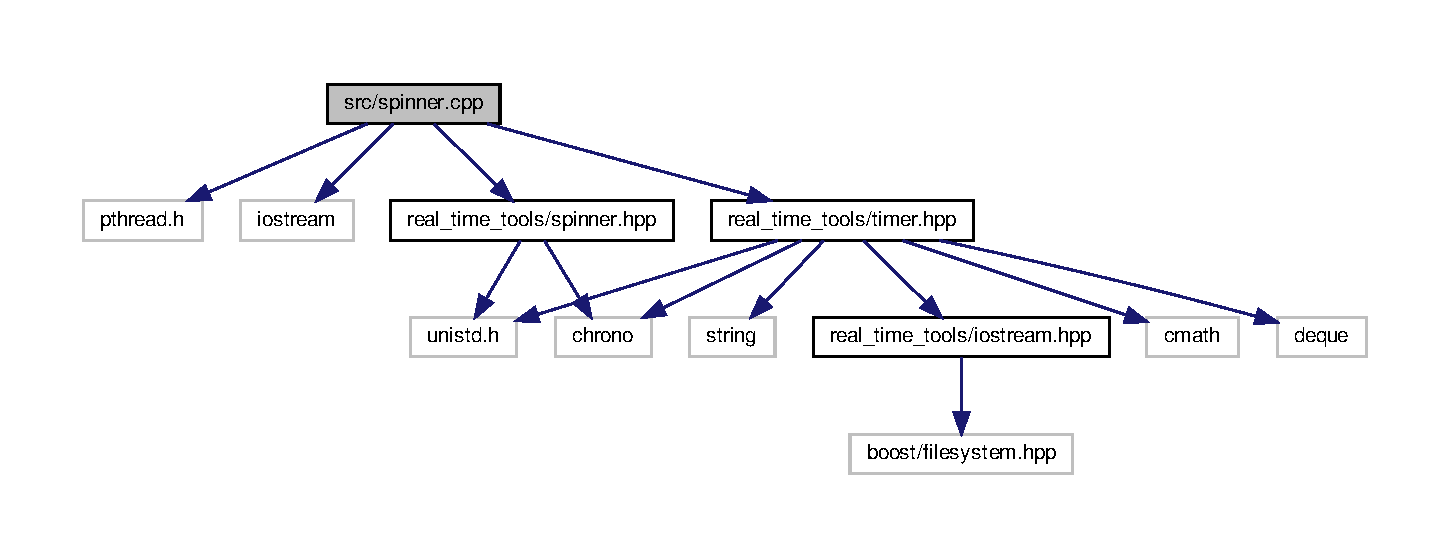
\includegraphics[width=350pt]{spinner_8cpp__incl}
\end{center}
\end{figure}


\subsection{Detailed Description}
This file implements a spinner to time a loop. 

\begin{DoxyAuthor}{Author}
Maximilien Naveau (\href{mailto:maximilien.naveau@gmail.com}{\tt maximilien.\+naveau@gmail.\+com}) license License B\+S\+D-\/3-\/\+Clause 
\end{DoxyAuthor}
\begin{DoxyCopyright}{Copyright}
Copyright (c) 2019, New York University and Max Planck Gesellschaft. 
\end{DoxyCopyright}
\begin{DoxyDate}{Date}
2019-\/05-\/22 
\end{DoxyDate}

\hypertarget{thread_8cpp}{}\section{src/thread.cpp File Reference}
\label{thread_8cpp}\index{src/thread.\+cpp@{src/thread.\+cpp}}


Implement method to create and join threads.  


{\ttfamily \#include \char`\"{}real\+\_\+time\+\_\+tools/thread.\+hpp\char`\"{}}\newline
{\ttfamily \#include $<$stdexcept$>$}\newline
{\ttfamily \#include \char`\"{}real\+\_\+time\+\_\+tools/process\+\_\+manager.\+hpp\char`\"{}}\newline
Include dependency graph for thread.\+cpp\+:
\nopagebreak
\begin{figure}[H]
\begin{center}
\leavevmode
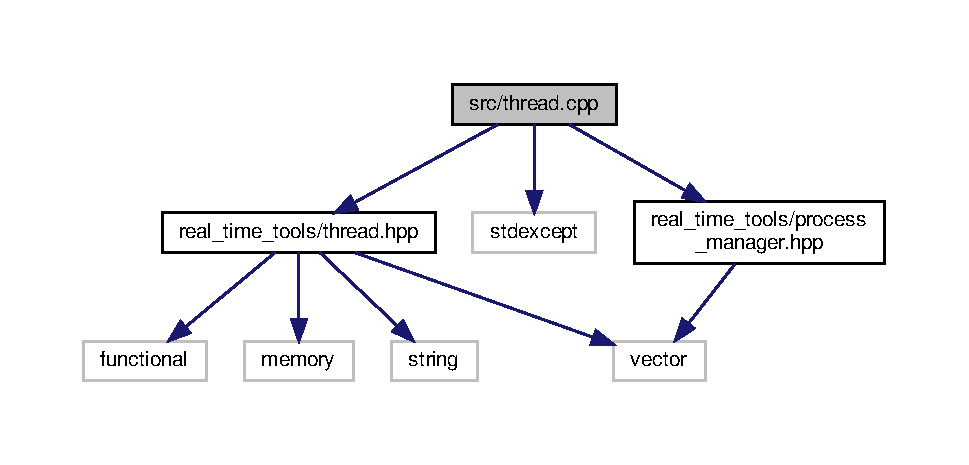
\includegraphics[width=350pt]{thread_8cpp__incl}
\end{center}
\end{figure}


\subsection{Detailed Description}
Implement method to create and join threads. 

\begin{DoxyAuthor}{Author}
Maximilien Naveau (\href{mailto:maximilien.naveau@gmail.com}{\tt maximilien.\+naveau@gmail.\+com}) license License B\+S\+D-\/3-\/\+Clause 
\end{DoxyAuthor}
\begin{DoxyCopyright}{Copyright}
Copyright (c) 2019, New York University and Max Planck Gesellschaft. 
\end{DoxyCopyright}
\begin{DoxyDate}{Date}
2019-\/05-\/22 
\end{DoxyDate}

\hypertarget{timer_8cpp}{}\section{src/timer.cpp File Reference}
\label{timer_8cpp}\index{src/timer.\+cpp@{src/timer.\+cpp}}


This file implements tools to acquire the time, the date, and do timing measurement.  


{\ttfamily \#include $<$time.\+h$>$}\newline
{\ttfamily \#include $<$fstream$>$}\newline
{\ttfamily \#include $<$iomanip$>$}\newline
{\ttfamily \#include $<$real\+\_\+time\+\_\+tools/iostream.\+hpp$>$}\newline
{\ttfamily \#include $<$real\+\_\+time\+\_\+tools/timer.\+hpp$>$}\newline
{\ttfamily \#include $<$sstream$>$}\newline
Include dependency graph for timer.\+cpp\+:
\nopagebreak
\begin{figure}[H]
\begin{center}
\leavevmode
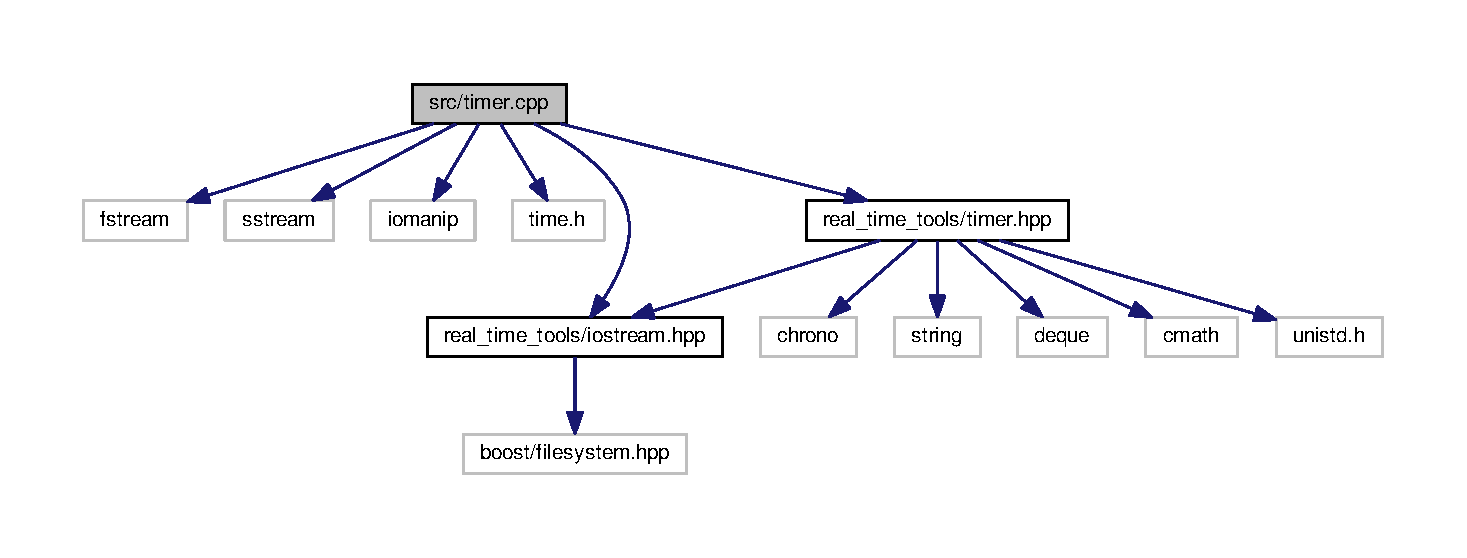
\includegraphics[width=350pt]{timer_8cpp__incl}
\end{center}
\end{figure}
\subsection*{Typedefs}
\begin{DoxyCompactItemize}
\item 
\mbox{\Hypertarget{timer_8cpp_a4481ea2a14fb44cfe1bf76fc43357b59}\label{timer_8cpp_a4481ea2a14fb44cfe1bf76fc43357b59}} 
typedef std\+::chrono\+::duration$<$ int, std\+::ratio\+\_\+multiply$<$ std\+::chrono\+::hours\+::period, std\+::ratio$<$ 24 $>$ $>$\+::type $>$ \hyperlink{timer_8cpp_a4481ea2a14fb44cfe1bf76fc43357b59}{real\+\_\+time\+\_\+tools\+::days}
\begin{DoxyCompactList}\small\item\em Simple renaming to get the number of days passed out of the date. \end{DoxyCompactList}\end{DoxyCompactItemize}


\subsection{Detailed Description}
This file implements tools to acquire the time, the date, and do timing measurement. 

\begin{DoxyAuthor}{Author}
Maximilien Naveau (\href{mailto:maximilien.naveau@gmail.com}{\tt maximilien.\+naveau@gmail.\+com}) license License B\+S\+D-\/3-\/\+Clause 
\end{DoxyAuthor}
\begin{DoxyCopyright}{Copyright}
Copyright (c) 2019, New York University and Max Planck Gesellschaft. 
\end{DoxyCopyright}
\begin{DoxyDate}{Date}
2019-\/05-\/22 
\end{DoxyDate}

\chapter{Example Documentation}
\hypertarget{demo_checkpoint_timer_8cpp-example}{}\section{demo\+\_\+checkpoint\+\_\+timer.\+cpp}
Demo on how to use the Checkpoint\+Timer.\+Note that when the statistics are printed like this, the printing is included in the time measurement of the total loop duration.


\begin{DoxyCodeInclude}

\textcolor{preprocessor}{#include <\hyperlink{checkpoint__timer_8hpp}{real\_time\_tools/checkpoint\_timer.hpp}>}
\textcolor{preprocessor}{#include <\hyperlink{timer_8hpp}{real\_time\_tools/timer.hpp}>}


\textcolor{keywordtype}{void} \hyperlink{demo__checkpoint__timer_8cpp_a02fd73d861ef2e4aabb38c0c9ff82947}{init}()
\{
    \hyperlink{classreal__time__tools_1_1Timer_abb2ce808994282d63846e7fca544f818}{real\_time\_tools::Timer::sleep\_ms}(3);
\}
\textcolor{keywordtype}{void} \hyperlink{demo__checkpoint__timer_8cpp_acb546a895e868f1a8fb9cb4b5a210f42}{do\_some\_stuff}()
\{
    \hyperlink{classreal__time__tools_1_1Timer_abb2ce808994282d63846e7fca544f818}{real\_time\_tools::Timer::sleep\_ms}(20);
\}
\textcolor{keywordtype}{void} \hyperlink{demo__checkpoint__timer_8cpp_a609e6537df0c7eb15c1f5b4e02fbe0ed}{write\_log}()
\{
    \hyperlink{classreal__time__tools_1_1Timer_abb2ce808994282d63846e7fca544f818}{real\_time\_tools::Timer::sleep\_ms}(6);
\}

\textcolor{keywordtype}{int} \hyperlink{demo__checkpoint__timer_8cpp_ae66f6b31b5ad750f1fe042a706a4e3d4}{main}()
\{

    \textcolor{comment}{// set second template argument to false to disable timer}
    \hyperlink{classreal__time__tools_1_1CheckpointTimer}{real\_time\_tools::CheckpointTimer<3, true>} timer;

    \textcolor{keywordflow}{for} (\textcolor{keywordtype}{int} i = 0; i < 1000; i++)
    \{
        timer.\hyperlink{classreal__time__tools_1_1CheckpointTimer_ad93a12cb74103528c8db4e7b1745eae6}{start}();

        \hyperlink{demo__checkpoint__timer_8cpp_a02fd73d861ef2e4aabb38c0c9ff82947}{init}();
        timer.\hyperlink{classreal__time__tools_1_1CheckpointTimer_a6e91b61b72c433a220b1bddb7a634bf5}{checkpoint}(\textcolor{stringliteral}{"initialize"});

        \hyperlink{demo__checkpoint__timer_8cpp_acb546a895e868f1a8fb9cb4b5a210f42}{do\_some\_stuff}();
        timer.\hyperlink{classreal__time__tools_1_1CheckpointTimer_a6e91b61b72c433a220b1bddb7a634bf5}{checkpoint}(\textcolor{stringliteral}{"do some stuff"});

        \hyperlink{demo__checkpoint__timer_8cpp_a609e6537df0c7eb15c1f5b4e02fbe0ed}{write\_log}();
        timer.\hyperlink{classreal__time__tools_1_1CheckpointTimer_a6e91b61b72c433a220b1bddb7a634bf5}{checkpoint}(\textcolor{stringliteral}{"logging"});

        \textcolor{comment}{// print the timing results every 100 iterations}
        \textcolor{keywordflow}{if} (i % 100 == 0 && i > 0)
        \{
            timer.\hyperlink{classreal__time__tools_1_1CheckpointTimer_acce8c21123fe6f450c8f22de575cfef8}{print\_statistics}();
        \}
    \}

    \textcolor{keywordflow}{return} 0;
\}
\end{DoxyCodeInclude}
 
\hypertarget{demo_realtime_check_8cpp-example}{}\section{demo\+\_\+realtime\+\_\+check.\+cpp}
This demos has for purpose to present the class \hyperlink{classreal__time__tools_1_1RealTimeCheck}{real\+\_\+time\+\_\+tools\+::\+Real\+Time\+Check}. This class measures the frequency of a loop and compares it with a threshold frequency. As demonstrated below, the class takes as input the desired frequency and the threshold frequency.

In order to enable the measurement of the your loop one need to call the \hyperlink{classreal__time__tools_1_1RealTimeCheck_a83fdf97352d36aa20e482d7dfae442d5}{real\+\_\+time\+\_\+tools\+::\+Real\+Time\+Check\+::tick()} function.

Finally the statistical results can be displayed via the \hyperlink{classreal__time__tools_1_1RealTimeCheck_a9c9c68da79843098085204095286a143}{real\+\_\+time\+\_\+tools\+::\+Real\+Time\+Check\+::print()} methods.


\begin{DoxyCodeInclude}

\textcolor{preprocessor}{#include "\hyperlink{timer_8hpp}{real\_time\_tools/timer.hpp}"}
\textcolor{preprocessor}{#include "\hyperlink{realtime__check_8hpp}{real\_time\_tools/realtime\_check.hpp}"}
\textcolor{preprocessor}{#include "\hyperlink{thread_8hpp}{real\_time\_tools/thread.hpp}"}

THREAD\_FUNCTION\_RETURN\_TYPE \hyperlink{demo__realtime__check_8cpp_a16919b2a4211953c87d405d40b432427}{thread\_function}(\textcolor{keywordtype}{void}*)
\{
  \textcolor{keywordtype}{double} freq = 1000.0; \textcolor{comment}{// 1kz}
  \textcolor{keywordtype}{double} switch\_freq = 990;
  \hyperlink{classreal__time__tools_1_1RealTimeCheck}{real\_time\_tools::RealTimeCheck} rc(freq,switch\_freq);
  \textcolor{keywordtype}{int} nb\_iteration = 10000;
  \textcolor{keywordtype}{int} a = 0;

  printf(\textcolor{stringliteral}{"sleeping time is %f seconds"}, 1.0/freq);

  \textcolor{keywordflow}{for}(\textcolor{keywordtype}{int} i=0 ; i<nb\_iteration ; ++i)\{
    rc.\hyperlink{classreal__time__tools_1_1RealTimeCheck_a83fdf97352d36aa20e482d7dfae442d5}{tick}();
    a++;
    \hyperlink{classreal__time__tools_1_1Timer_a0a0df8a3baef34e820203e5579afda38}{real\_time\_tools::Timer::sleep\_sec}(1.0/freq); \textcolor{comment}{// microseconds, so in
       Ghz}
  \}

  printf(\textcolor{stringliteral}{"\(\backslash\)n"});
  rc.\hyperlink{classreal__time__tools_1_1RealTimeCheck_a9c9c68da79843098085204095286a143}{print}();
  printf(\textcolor{stringliteral}{"\(\backslash\)n"});

  \textcolor{keywordflow}{return} THREAD\_FUNCTION\_RETURN\_VALUE;
\}

\textcolor{keywordtype}{int} \hyperlink{demo__realtime__check_8cpp_a81ce304348a420752ee080480d2b3095}{main}(\textcolor{keywordtype}{int} , \textcolor{keywordtype}{char}* []) \{
  \hyperlink{classreal__time__tools_1_1RealTimeThread}{real\_time\_tools::RealTimeThread} thread;
  thread.\hyperlink{classreal__time__tools_1_1RealTimeThread_a232e3955fee6e80c3a7ded68f165414b}{create\_realtime\_thread}(\hyperlink{demo__realtime__check_8cpp_a16919b2a4211953c87d405d40b432427}{thread\_function});
  thread.\hyperlink{classreal__time__tools_1_1RealTimeThread_a2f455db9fd80b81e5e69cd22e8529979}{join}();
\}

\end{DoxyCodeInclude}
 
\hypertarget{demo_realtime_strict_check_8cpp-example}{}\section{demo\+\_\+realtime\+\_\+strict\+\_\+check.\+cpp}
This demos has for purpose to present the class \hyperlink{classreal__time__tools_1_1RealTimeCheck}{real\+\_\+time\+\_\+tools\+::\+Real\+Time\+Check}. This class measures the frequency of a loop and compares it with a threshold frequency. As demonstrated below, the class takes as input the desired frequency and the threshold frequency.

In order to enable the measurement of the your loop one need to call the \hyperlink{classreal__time__tools_1_1RealTimeCheck_a83fdf97352d36aa20e482d7dfae442d5}{real\+\_\+time\+\_\+tools\+::\+Real\+Time\+Check\+::tick()} function.

Finally the statistical results can be displayed via the \hyperlink{classreal__time__tools_1_1RealTimeCheck_a9c9c68da79843098085204095286a143}{real\+\_\+time\+\_\+tools\+::\+Real\+Time\+Check\+::print()} methods.

The difference with the \hyperlink{demo__realtime__check_8cpp}{demo\+\_\+realtime\+\_\+check.\+cpp} is that we measure the sleeping time as well.


\begin{DoxyCodeInclude}

\textcolor{preprocessor}{#include "\hyperlink{realtime__check_8hpp}{real\_time\_tools/realtime\_check.hpp}"}
\textcolor{preprocessor}{#include "\hyperlink{thread_8hpp}{real\_time\_tools/thread.hpp}"}

\textcolor{keyword}{typedef} std::chrono::high\_resolution\_clock \hyperlink{demo__realtime__strict__check_8cpp_a3b195616f5dbd3a9cae7f618efe85b9b}{my\_clock};

THREAD\_FUNCTION\_RETURN\_TYPE \hyperlink{demo__realtime__strict__check_8cpp_a16919b2a4211953c87d405d40b432427}{thread\_function}(\textcolor{keywordtype}{void}*)
\{
  \textcolor{keywordtype}{double} freq = 1000.0; \textcolor{comment}{// 1kz}
  \textcolor{keywordtype}{double} switch\_freq = 990;
  \textcolor{keywordtype}{int} nb\_iteration = 1000;

  \textcolor{keywordtype}{unsigned} period = \textcolor{keyword}{static\_cast<}\textcolor{keywordtype}{unsigned}\textcolor{keyword}{>}(round((1.0/freq) * pow(10.0, 9.0)));
  my\_clock::duration clock\_period(period);
  \hyperlink{classreal__time__tools_1_1RealTimeCheck}{real\_time\_tools::RealTimeCheck} rc(freq,switch\_freq);
  \textcolor{keywordtype}{int} a = 0;
  my\_clock::time\_point start, \hyperlink{realtime__test_8cpp_aba399b0a6a6e3bd37af95bd04e8def6f}{stop}, mid;
  my\_clock::duration sleep\_duration\_diff;
  \textcolor{keyword}{struct }timespec sleep\_duration, out\_sleep;

  printf(\textcolor{stringliteral}{"reference period is %ld\(\backslash\)n"}, clock\_period.count());

  \textcolor{keywordflow}{for}(\textcolor{keywordtype}{int} i=0 ; i<nb\_iteration ; ++i)\{
    start = my\_clock::now();

    rc.\hyperlink{classreal__time__tools_1_1RealTimeCheck_a83fdf97352d36aa20e482d7dfae442d5}{tick}();


    a++;
    \textcolor{comment}{//printf("%d %d", sleep\_duration.tv\_nsec, out\_sleep.tv\_nsec);}
    \textcolor{comment}{//printf("%ld ; %ld ; ", sleep\_duration.tv\_nsec, sleep\_duration\_diff.count());}
    \textcolor{comment}{//printf("sleeping time is %ld  \(\backslash\)n", sleep\_duration.tv\_nsec);}

    mid = my\_clock::now();
    sleep\_duration.tv\_nsec = (clock\_period -
                              sleep\_duration\_diff -
                              (mid - start)).count();

    nanosleep(&sleep\_duration, &out\_sleep); \textcolor{comment}{// microseconds, so in Ghz}

    stop = my\_clock::now();
    sleep\_duration\_diff = my\_clock::duration(
          (\textcolor{keywordtype}{unsigned}) ((stop - mid) - my\_clock::duration(
                        sleep\_duration.tv\_nsec)).count());
  \}

  printf(\textcolor{stringliteral}{"\(\backslash\)n"});
  rc.\hyperlink{classreal__time__tools_1_1RealTimeCheck_a9c9c68da79843098085204095286a143}{print}();
  printf(\textcolor{stringliteral}{"\(\backslash\)n"});

  \textcolor{keywordflow}{return} THREAD\_FUNCTION\_RETURN\_VALUE;
\}

\textcolor{keywordtype}{int} \hyperlink{demo__realtime__strict__check_8cpp_a81ce304348a420752ee080480d2b3095}{main}(\textcolor{keywordtype}{int} , \textcolor{keywordtype}{char}* []) \{
  \hyperlink{classreal__time__tools_1_1RealTimeThread}{real\_time\_tools::RealTimeThread} thread;
  thread.\hyperlink{classreal__time__tools_1_1RealTimeThread_a232e3955fee6e80c3a7ded68f165414b}{create\_realtime\_thread}(\hyperlink{demo__realtime__strict__check_8cpp_a16919b2a4211953c87d405d40b432427}{thread\_function});
  thread.\hyperlink{classreal__time__tools_1_1RealTimeThread_a2f455db9fd80b81e5e69cd22e8529979}{join}();
\}

\end{DoxyCodeInclude}
 
\hypertarget{demo_spinner_8cpp-example}{}\section{demo\+\_\+spinner.\+cpp}
This demos has for purpose to present the class real\+\_\+time\+\_\+tools\+::\+Spinner.\+This class allows you to time a loop with a simple A\+PI.

One need to create a spinner and set the current spinning frequency. Two method are available for this\+: \hyperlink{classreal__time__tools_1_1Spinner_afa4e24e5dbbbfa2e0d694ef2e3fa3bb8}{real\+\_\+time\+\_\+tools\+::\+Spinner\+::set\+\_\+frequency()} or \hyperlink{classreal__time__tools_1_1Spinner_ac945d6df02f33e75f499922d23838408}{real\+\_\+time\+\_\+tools\+::\+Spinner\+::set\+\_\+period()}..

Once this is set one just needs to call \hyperlink{classreal__time__tools_1_1Spinner_aa07d4fa32ead44008daa73663508139d}{real\+\_\+time\+\_\+tools\+::\+Spinner\+::spin()} and the thread will sleep just the amount of time needed in order for the loop to cadenced properly.


\begin{DoxyCodeInclude}

\textcolor{preprocessor}{#include "\hyperlink{realtime__check_8hpp}{real\_time\_tools/realtime\_check.hpp}"}
\textcolor{preprocessor}{#include "\hyperlink{spinner_8hpp}{real\_time\_tools/spinner.hpp}"}
\textcolor{preprocessor}{#include "\hyperlink{thread_8hpp}{real\_time\_tools/thread.hpp}"}

THREAD\_FUNCTION\_RETURN\_TYPE \hyperlink{demo__spinner_8cpp_a16919b2a4211953c87d405d40b432427}{thread\_function}(\textcolor{keywordtype}{void}*)
\{
    \textcolor{keywordtype}{double} frequency = 300.0;
    \textcolor{keywordtype}{double} switch\_frequency = 290;

    \hyperlink{classreal__time__tools_1_1RealTimeCheck}{real\_time\_tools::RealTimeCheck} realtime\_check(frequency, switch\_frequency
      );
    \hyperlink{classreal__time__tools_1_1Spinner}{real\_time\_tools::Spinner} spinner;
    spinner.\hyperlink{classreal__time__tools_1_1Spinner_afa4e24e5dbbbfa2e0d694ef2e3fa3bb8}{set\_frequency}(frequency);

    \textcolor{keywordflow}{for} (\textcolor{keywordtype}{int} i = 0; i < 500; i++)
    \{
        realtime\_check.\hyperlink{classreal__time__tools_1_1RealTimeCheck_a83fdf97352d36aa20e482d7dfae442d5}{tick}();
        spinner.\hyperlink{classreal__time__tools_1_1Spinner_aa07d4fa32ead44008daa73663508139d}{spin}();
    \}

    std::cout << \textcolor{stringliteral}{"\(\backslash\)n"};
    realtime\_check.\hyperlink{classreal__time__tools_1_1RealTimeCheck_a9c9c68da79843098085204095286a143}{print}();
    std::cout << \textcolor{stringliteral}{"\(\backslash\)n"};

    \textcolor{keywordflow}{return} THREAD\_FUNCTION\_RETURN\_VALUE;
\}

\textcolor{keywordtype}{int} \hyperlink{demo__spinner_8cpp_a81ce304348a420752ee080480d2b3095}{main}(\textcolor{keywordtype}{int}, \textcolor{keywordtype}{char}* [])
\{
    \hyperlink{classreal__time__tools_1_1RealTimeThread}{real\_time\_tools::RealTimeThread} thread;
    thread.\hyperlink{classreal__time__tools_1_1RealTimeThread_a232e3955fee6e80c3a7ded68f165414b}{create\_realtime\_thread}(\hyperlink{demo__spinner_8cpp_a16919b2a4211953c87d405d40b432427}{thread\_function});
    thread.\hyperlink{classreal__time__tools_1_1RealTimeThread_a2f455db9fd80b81e5e69cd22e8529979}{join}();
\}

\end{DoxyCodeInclude}
 
\hypertarget{demo_timing_8cpp-example}{}\section{demo\+\_\+timing.\+cpp}
This demos has for purpose to present the class real\+\_\+time\+\_\+tools\+::\+Timer.\+This class allows you to use the real time clocks. And measure durations and extract statistics on them.

Inn this example we create a simple loop cadence by the \hyperlink{classreal__time__tools_1_1Spinner}{real\+\_\+time\+\_\+tools\+::\+Spinner}. And we measure the period of the loop.

In order to do so one need to create a \hyperlink{classreal__time__tools_1_1Timer}{real\+\_\+time\+\_\+tools\+::\+Timer} and call the \hyperlink{classreal__time__tools_1_1Timer_a310fc3b9165c3751a36ff92586f0facd}{real\+\_\+time\+\_\+tools\+::\+Timer\+::tac\+\_\+tic()} method which compute the duration between each call of this method.

The demo displays the statistics of the measured time every milliseconds.


\begin{DoxyCodeInclude}

\textcolor{preprocessor}{#include "\hyperlink{spinner_8hpp}{real\_time\_tools/spinner.hpp}"}
\textcolor{preprocessor}{#include "\hyperlink{thread_8hpp}{real\_time\_tools/thread.hpp}"}
\textcolor{preprocessor}{#include "\hyperlink{realtime__check_8hpp}{real\_time\_tools/realtime\_check.hpp}"}
\textcolor{preprocessor}{#include "\hyperlink{timer_8hpp}{real\_time\_tools/timer.hpp}"}

THREAD\_FUNCTION\_RETURN\_TYPE \hyperlink{demo__timing_8cpp_a16919b2a4211953c87d405d40b432427}{thread\_function}(\textcolor{keywordtype}{void}*)
\{

    \textcolor{keywordtype}{double} frequency = 1000;

    \hyperlink{classreal__time__tools_1_1Spinner}{real\_time\_tools::Spinner} spinner;
    spinner.\hyperlink{classreal__time__tools_1_1Spinner_afa4e24e5dbbbfa2e0d694ef2e3fa3bb8}{set\_frequency}(frequency);

    \hyperlink{classreal__time__tools_1_1Timer}{real\_time\_tools::Timer} timer;

    \textcolor{keywordflow}{while}(\textcolor{keyword}{true})
    \{
        \textcolor{keywordflow}{for}(\textcolor{keywordtype}{int} i = 0; i < frequency; i++)
        \{
            spinner.\hyperlink{classreal__time__tools_1_1Spinner_aa07d4fa32ead44008daa73663508139d}{spin}();
            timer.\hyperlink{classreal__time__tools_1_1Timer_a310fc3b9165c3751a36ff92586f0facd}{tac\_tic}();
        \}

        timer.\hyperlink{classreal__time__tools_1_1Timer_a16635bb883c6f71772093a89cbe3130a}{print\_statistics}();
    \}

    \textcolor{keywordflow}{return} THREAD\_FUNCTION\_RETURN\_VALUE;
\}

\textcolor{keywordtype}{int} \hyperlink{demo__timing_8cpp_a81ce304348a420752ee080480d2b3095}{main}(\textcolor{keywordtype}{int} , \textcolor{keywordtype}{char}* []) \{
  \hyperlink{classreal__time__tools_1_1RealTimeThread}{real\_time\_tools::RealTimeThread} thread;
  thread.\hyperlink{classreal__time__tools_1_1RealTimeThread_a232e3955fee6e80c3a7ded68f165414b}{create\_realtime\_thread}(\hyperlink{demo__timing_8cpp_a16919b2a4211953c87d405d40b432427}{thread\_function});
  thread.\hyperlink{classreal__time__tools_1_1RealTimeThread_a2f455db9fd80b81e5e69cd22e8529979}{join}();
\}

\end{DoxyCodeInclude}
 
\hypertarget{demo_usb_stream_imu_3DM_GX3_25_8cpp-example}{}\section{demo\+\_\+usb\+\_\+stream\+\_\+imu\+\_\+3\+D\+M\+\_\+\+G\+X3\+\_\+25.\+cpp}
In order to use this Demo one must have an I\+MU 3\+D\+M-\/\+G\+X3-\/25 from micro-\/strain plug in one of the usb port of the computer.\+https\+://atlas.is.\+localnet/confluence/display/\+A\+M\+D\+W/\+Microstrain+3\+D\+M+\+I\+M\+Us?preview=/8979810/17761244/3\+D\+M-\/\+G\+X3-\/\+Data-\/\+Communications-\/\+Protocol.pdf

This demos present the use of the usb socket use using the real\+\_\+time\+\_\+tools A\+PI.

One need to create a \hyperlink{classreal__time__tools_1_1UsbStream}{real\+\_\+time\+\_\+tools\+::\+Usb\+Stream}. This class allows you to open a device, which means that the class connects this process to a usb communication socket.\+One can initialize the socket parameters through the \hyperlink{classreal__time__tools_1_1PortConfig}{real\+\_\+time\+\_\+tools\+::\+Port\+Config} structure. Once open one can simply use the communication protocole of the hardware to send and receive messages.


\begin{DoxyCodeInclude}

\textcolor{preprocessor}{#include "\hyperlink{timer_8hpp}{real\_time\_tools/timer.hpp}"}
\textcolor{preprocessor}{#include "real\_time\_tools/usb\_stream.hpp"}

\textcolor{keywordtype}{void} \hyperlink{demo__usb__stream__imu__3DM__GX3__25_8cpp_af411ef352aef0f8d040d8d60c49eac7a}{continuous\_mode\_on}(\hyperlink{classreal__time__tools_1_1UsbStream}{real\_time\_tools::UsbStream}& usb\_stream,
                        \textcolor{keywordtype}{bool} stream\_mode)
\{
    std::vector<uint8\_t> reply;
    std::vector<uint8\_t> command;

    command.resize(4);
    command[0] = 0xc4;  \textcolor{comment}{// set continuous mode on}
    command[1] = 0xc1;  \textcolor{comment}{// user confirmation 1}
    command[2] = 0x29;  \textcolor{comment}{// user confirmation 2}
    command[3] =
        0xc2;  \textcolor{comment}{// Acceleration and angular rate continuously broadcasted}
    reply.resize(8, 0);  \textcolor{comment}{// answer in 8 bits.}

    rt\_printf(\textcolor{stringliteral}{"The IMU will blink fast\(\backslash\)n"});
    \textcolor{keywordflow}{while} (!(reply[0] == 0xC4 && reply[1] == 0xc2))
    \{
        usb\_stream.\hyperlink{classreal__time__tools_1_1UsbStream_aa9fdd0d43fbf0cddbffb65538af60321}{write\_device}(command);
        usb\_stream.\hyperlink{classreal__time__tools_1_1UsbStream_a028f39fcd8c97c49aacf48fdaa8302c8}{read\_device}(reply, stream\_mode);
    \}
    rt\_printf(\textcolor{stringliteral}{"Device answer is: %s\(\backslash\)n"},
              \hyperlink{classreal__time__tools_1_1UsbStream_ac98f3cad23dbc85f47405c3809a22198}{real\_time\_tools::UsbStream::msg\_debug\_string}(
      reply).c\_str());
    rt\_printf(\textcolor{stringliteral}{"The IMU should blink fast\(\backslash\)n"});
\}

\textcolor{keywordtype}{bool} \hyperlink{demo__usb__stream__imu__3DM__GX3__25_8cpp_a8a096d7f567dad6d28f0fd870ba6bb43}{is\_continuous\_mode\_on}(\hyperlink{classreal__time__tools_1_1UsbStream}{real\_time\_tools::UsbStream}& 
      usb\_stream,
                           \textcolor{keywordtype}{bool} stream\_mode)
\{
    std::vector<uint8\_t> reply;
    std::vector<uint8\_t> command;

    command.resize(4);
    command[0] = 0xd4;   \textcolor{comment}{// set continuous mode on}
    command[1] = 0xa3;   \textcolor{comment}{// user confirmation 1}
    command[2] = 0x47;   \textcolor{comment}{// user confirmation 2}
    command[3] = 0;      \textcolor{comment}{// request continuous mode}
    reply.resize(4, 0);  \textcolor{comment}{// answer in 8 bits.}

    \textcolor{keywordtype}{bool} success = usb\_stream.\hyperlink{classreal__time__tools_1_1UsbStream_aa9fdd0d43fbf0cddbffb65538af60321}{write\_device}(command);
    success = success && usb\_stream.\hyperlink{classreal__time__tools_1_1UsbStream_a028f39fcd8c97c49aacf48fdaa8302c8}{read\_device}(reply, stream\_mode);
    rt\_printf(\textcolor{stringliteral}{"is continuous mode reply: %s\(\backslash\)n"},
              \hyperlink{classreal__time__tools_1_1UsbStream_ac98f3cad23dbc85f47405c3809a22198}{real\_time\_tools::UsbStream::msg\_debug\_string}(
      reply).c\_str());
    \textcolor{keywordflow}{return} success && (reply[1] > 0);
\}

\textcolor{keywordtype}{void} \hyperlink{demo__usb__stream__imu__3DM__GX3__25_8cpp_a1d00f7ae49ec05ecaf8ecd4d76129573}{continuous\_mode\_off}(\hyperlink{classreal__time__tools_1_1UsbStream}{real\_time\_tools::UsbStream}& 
      usb\_stream,
                         \textcolor{keywordtype}{bool} stream\_mode)
\{
    std::vector<uint8\_t> reply;
    std::vector<uint8\_t> command;

    command.resize(4);
    command[0] = 0xc4;  \textcolor{comment}{// set continuous mode on}
    command[1] = 0xc1;  \textcolor{comment}{// user confirmation 1}
    command[2] = 0x29;  \textcolor{comment}{// user confirmation 2}
    command[3] =
        0x00;  \textcolor{comment}{// Acceleration and angular rate continuously broadcasted}
    reply.resize(8, 0xFF);  \textcolor{comment}{// answer in 8 bits.}

    rt\_printf(\textcolor{stringliteral}{"The IMU will blink slowly\(\backslash\)n"});
    \textcolor{keywordflow}{while} (!(reply[0] == 0xC4 && reply[1] == 0x00))
    \{
        usb\_stream.\hyperlink{classreal__time__tools_1_1UsbStream_aa9fdd0d43fbf0cddbffb65538af60321}{write\_device}(command);
        usb\_stream.\hyperlink{classreal__time__tools_1_1UsbStream_a028f39fcd8c97c49aacf48fdaa8302c8}{read\_device}(reply, stream\_mode);
    \}
    rt\_printf(\textcolor{stringliteral}{"Device answer is: %s\(\backslash\)n"},
              \hyperlink{classreal__time__tools_1_1UsbStream_ac98f3cad23dbc85f47405c3809a22198}{real\_time\_tools::UsbStream::msg\_debug\_string}(
      reply).c\_str());
    rt\_printf(\textcolor{stringliteral}{"The IMU should blink slowly\(\backslash\)n"});
\}

\textcolor{keywordtype}{void} \hyperlink{demo__usb__stream__imu__3DM__GX3__25_8cpp_af04ed9328c659fc57f91d74cdeedda72}{reset}(\hyperlink{classreal__time__tools_1_1UsbStream}{real\_time\_tools::UsbStream}& usb\_stream, \textcolor{keywordtype}{bool} stream\_mode)
\{
    std::vector<uint8\_t> reply;
    std::vector<uint8\_t> command;

    command.resize(3);
    command[0] = 0xfe;   \textcolor{comment}{// reset device}
    command[1] = 0x9e;   \textcolor{comment}{// user confirmation 1}
    command[2] = 0x3a;   \textcolor{comment}{// user confirmation 2}
    reply.resize(0, 0);  \textcolor{comment}{// answer in 8 bits.}

    rt\_printf(\textcolor{stringliteral}{"The IMU is resetting\(\backslash\)n"});
    usb\_stream.\hyperlink{classreal__time__tools_1_1UsbStream_aa9fdd0d43fbf0cddbffb65538af60321}{write\_device}(command);
    usb\_stream.\hyperlink{classreal__time__tools_1_1UsbStream_a028f39fcd8c97c49aacf48fdaa8302c8}{read\_device}(reply, stream\_mode);
    rt\_printf(\textcolor{stringliteral}{"Device answer is: %s\(\backslash\)n"},
              \hyperlink{classreal__time__tools_1_1UsbStream_ac98f3cad23dbc85f47405c3809a22198}{real\_time\_tools::UsbStream::msg\_debug\_string}(
      reply).c\_str());
    rt\_printf(\textcolor{stringliteral}{"The IMU is reset\(\backslash\)n"});
    \hyperlink{classreal__time__tools_1_1Timer_a0a0df8a3baef34e820203e5579afda38}{real\_time\_tools::Timer::sleep\_sec}(10);
\}

\textcolor{keywordtype}{int} \hyperlink{demo__usb__stream__imu__3DM__GX3__25_8cpp_a3c04138a5bfe5d72780bb7e82a18e627}{main}(\textcolor{keywordtype}{int} argc, \textcolor{keywordtype}{char}** argv)
\{
    \textcolor{keywordflow}{if} (argc != 2)
    \{
        printf(\textcolor{stringliteral}{"usage: demo\_device\_stream <device>\(\backslash\)ne.g. %s /dev/tty0\(\backslash\)n"},
               argv[0]);
        \textcolor{keywordflow}{return} -1;
    \}

    \textcolor{comment}{// Let us acquire the device path from the application arguments}
    std::string device = std::string(argv[1]);

    \hyperlink{classreal__time__tools_1_1UsbStream}{real\_time\_tools::UsbStream} usb\_stream;

    \textcolor{keywordflow}{if} (!usb\_stream.\hyperlink{classreal__time__tools_1_1UsbStream_a1f6915c42d9742ced10e99d2edf7d8b1}{open\_device}(device))
    \{
        \textcolor{keywordflow}{return} -1;
    \}

    \hyperlink{classreal__time__tools_1_1PortConfig}{real\_time\_tools::PortConfig} port\_config;
    port\_config.\hyperlink{classreal__time__tools_1_1PortConfig_ad89a20459faf7718a63ea8c00ddc5e34}{rts\_cts\_enabled\_} = \textcolor{keyword}{false};
    port\_config.\hyperlink{classreal__time__tools_1_1PortConfig_afdc811c6c73ada4b21dab246bf086506}{parity\_} = \textcolor{keyword}{false};
    port\_config.\hyperlink{classreal__time__tools_1_1PortConfig_a3303d793237edbfa0b3c28f3f01c3837}{stop\_bits\_} = real\_time\_tools::PortConfig::StopBits::one;
    port\_config.\hyperlink{classreal__time__tools_1_1PortConfig_a6c1dbeb3cf3c772c9c1b4df71b8befd6}{prepare\_size\_definition\_} = \textcolor{keyword}{false};
    port\_config.\hyperlink{classreal__time__tools_1_1PortConfig_af80f9991e3811392385208a9baf9c6fd}{data\_bits\_} = real\_time\_tools::PortConfig::cs8;
    port\_config.\hyperlink{classreal__time__tools_1_1PortConfig_aa0be2d74f3ac70e9f43d36fc0c70901a}{baude\_rate\_} = 115200;
    usb\_stream.\hyperlink{classreal__time__tools_1_1UsbStream_adb0c41dc7a9603022a0a1e19c9ab8292}{set\_port\_config}(port\_config);
    usb\_stream.\hyperlink{classreal__time__tools_1_1UsbStream_a1c61741541acfca7ecf6deaf0b8ad1fc}{set\_poll\_mode\_timeout}(0.1);

    \textcolor{comment}{// stream mode of the usb port}
    \textcolor{keywordtype}{bool} stream\_mode = \textcolor{keyword}{false};

    \hyperlink{classreal__time__tools_1_1Timer_a0a0df8a3baef34e820203e5579afda38}{real\_time\_tools::Timer::sleep\_sec}(1);

    \hyperlink{demo__usb__stream__imu__3DM__GX3__25_8cpp_af411ef352aef0f8d040d8d60c49eac7a}{continuous\_mode\_on}(usb\_stream, stream\_mode);
    \hyperlink{classreal__time__tools_1_1Timer_a0a0df8a3baef34e820203e5579afda38}{real\_time\_tools::Timer::sleep\_sec}(5);

    usb\_stream.\hyperlink{classreal__time__tools_1_1UsbStream_a0bc5fb5783f1833341d55b9b013be6c6}{flush}();
    \hyperlink{demo__usb__stream__imu__3DM__GX3__25_8cpp_a1d00f7ae49ec05ecaf8ecd4d76129573}{continuous\_mode\_off}(usb\_stream, stream\_mode);
    usb\_stream.\hyperlink{classreal__time__tools_1_1UsbStream_a0bc5fb5783f1833341d55b9b013be6c6}{flush}();

    rt\_printf(\textcolor{stringliteral}{"Close port\(\backslash\)n"});
    usb\_stream.\hyperlink{classreal__time__tools_1_1UsbStream_acea75055bb37f2a7f351300dbaf28d9e}{close\_device}();

    rt\_printf(\textcolor{stringliteral}{"Stop program\(\backslash\)n"});
    \textcolor{keywordflow}{return} 0;
\}

\end{DoxyCodeInclude}
 
%--- End generated contents ---

% Index
\backmatter
\newpage
\phantomsection
\clearemptydoublepage
\addcontentsline{toc}{chapter}{Index}
\printindex

\end{document}
